\documentclass[11pt, a4paper, openany]{book}
\usepackage[utf8]{inputenc}
\usepackage[T2A]{fontenc}
\usepackage[russian,french]{babel}
\usepackage[style=authoryear]{biblatex}
\usepackage{graphicx}
\usepackage{amsmath, amsfonts}
\usepackage[most]{tcolorbox}
\usepackage[nomarginpar, left=3cm, right=3cm, top=3.5cm, bottom=4cm]{geometry}
%\usepackage[nomarginpar, left=0.5cm, right=0.5cm, top=0.5cm, bottom=0.5cm]{geometry}
\usepackage{listings}
\usepackage{xcolor}
\usepackage{xparse}
\usepackage{svg}
\usepackage{setspace}
\usepackage{hyperref}
\usepackage{palatino}
\usepackage{minted}
\usepackage[protrusion = true, final]{microtype}
\emergencystretch=1.5em
\usemintedstyle{pastie}
\setminted{breaklines, linenos, frame=lines, framesep=2mm, fontsize=\footnotesize}
\usepackage{csquotes}
\AtBeginDocument{\def\labelitemi{$\bullet$}}

\newcommand\dd{\mathrm d}
\newcommand\od[2]{\frac {\dd{#1}}{\dd{#2}}}
\renewcommand\nod[3]{\frac {\dd^{#3}{#1}}{\dd{#2}^{#3}}}
\newcommand\pd[2]{\frac {\partial {#1}}{\partial {#2}}}
\DeclareMathOperator\Tr{Tr}
\newcommand\robin[1]{{\textcolor{teal}{Robin~: #1}}}
%\renewcommand\robin[1]{}  % Décommenter pour masquer les remarques

\setstretch{1.2}
%\setstretch{0.7}

\definecolor{codegreen}{rgb}{0,0.6,0}
\definecolor{codered}{rgb}{0.75,0,0}
\definecolor{codegray}{rgb}{0.5,0.5,0.5}
\definecolor{codeblue}{rgb}{0,0.5,0.92}
\definecolor{backcolour}{rgb}{0.95,0.95,0.95}
\definecolor{definitionblue}{rgb}{0.34, 0.7, 1}
\definecolor{theoremred}{rgb}{0.7, 0.0, 0.3}
\definecolor{lemmagreen}{rgb}{0.0, 0.7, 0.3}
\definecolor{exercisepurple}{rgb}{0.5, 0.0, 0.5}

\NewDocumentCommand{\codeword}{v}{\texttt{\textcolor{codered}{#1}}}

\tcbset {
  base/.style={
    arc=0mm, 
    bottomtitle=0.5mm,
    boxrule=0mm,
    colbacktitle=black!10!white, 
    coltitle=black, 
    fonttitle=\bfseries, 
    left=2.5mm,
    leftrule=1mm,
    right=3.5mm,
    title={#1},
    toptitle=0.75mm, 
  }
}

\newtcolorbox{definitionbox}[1]{
  colframe=definitionblue, 
  base={#1}
}

\newtcolorbox{theorembox}[1]{
  colframe=theoremred, 
  base={#1}
}

\newtcolorbox{lemmabox}[1]{
  colframe=lemmagreen, 
  base={#1}
}

\newtcolorbox{exercisebox}[1]{
  colframe=exercisepurple, 
  base={#1}
}

\newtcolorbox{subbox}[1]{
  colframe=black!30!white,
  base={#1}
}

\newenvironment{definition}[1]{
    \begin{definitionbox}{#1}
}{
    \end{definitionbox}
}

\newenvironment{theorem}[1]{
    \begin{theorembox}{#1}
}{
    \end{theorembox}
}

\newenvironment{lemma}[1]{
    \begin{lemmabox}{#1}
}{
    \end{lemmabox}
}

\newenvironment{exercise}[1]{
    \begin{exercisebox}{#1}
}{
    \end{exercisebox}
}

\let\oldquote\quote
\let\endoldquote\endquote
\renewenvironment{quote}[2][]
  {\if\relax\detokenize{#1}\relax
     \def\quoteauthor{#2}%
   \else
     \def\quoteauthor{#2~---~#1}%
   \fi
   \oldquote}
  {\par\nobreak\smallskip\hfill(\quoteauthor)%
   \endoldquote\addvspace{\bigskipamount}}

\newcommand{\hide}[1]{}

\title{Syllabus d’exercices INFO-F-305\\Support au cours de Modélisation et Simulation}
\author{Pascal \textsc{Tribel}\\ %, Abel \textsc{Laval}\\
%Eythan \textsc{Levy}, 
Jacopo \textsc{De Stefani}\\
%Liran \textsc{Lerman}, 
Yannick \textsc{Molinghen}\\ 
Gianluca \textsc{Bontempi}\\
\\
Département d’Informatique, Faculté des Sciences\\
Université Libre de Bruxelles, ULB}
\date{\today}

\addbibresource{bibliographie.bib}

\begin{document}

\maketitle

\pagenumbering{roman}
\topskip0pt
\vspace*{\fill}
\begin{quote}{George Box, 1987}
    All models are wrong, but some are useful.
\end{quote}
\vspace*{\fill}
\chapter*{Avant-propos}
    Le présent document vise à offrir un support à l'étudiant·e dans la réalisation des exercices en séances de travaux pratiques pour le cours de Modélisation et Simulation donné en troisième année de bachelier à l'Université Libre de Bruxelles. Il sert de complément au syllabus du cours magistral, véritable outil de référence pour l'apprentissage.
    Le contenu de ce syllabus se base sur les ressources préexistantes, remises en forme et complétées d'explications et de mises en contextes historiques et scientifiques. L'objectif de ce texte est à la fois de donner à l'étudiant·e toutes les clés nécessaires à la réussite de la partie pratique du cours, mais surtout, de montrer l'étendue des possibilités offertes par le monde de la simulation numérique.

    Ce document n'est pas extensif: bon nombre de points n'y sont pas abordés, plusieurs autres sont supposés connus. L'étudiant·e est invité·e, avant tout, à se référer au syllabus principal, et à la documentation des outils présentés dans les différents chapitres.

    Les outils présentés étant en constante évolution, il n'est pas impossible que certains points présentés dans les prochains chapitres deviennent obsolètes; les auteurs, néanmoins, sont convaincus que la plupart des concepts entourant l'utilisation des outils spécifiques resteront utiles.

    Enfin, l'ouvrage est aussi à utiliser comme un \textit{mémo pratique}: les exercices résolus, les exemples illustrés, accompagnés des codes pour les générer, seront sûrement d'utilité non négligeable pour rapidement se remémorer les méthodes de résolution et de simulation.

    Nous voulons remercier, sans ordre d'importance, les personnes suivantes, pour la rédaction de ce document et pour les ressources mises à disposition: \textit{Gianluca Bontempi, Abel Laval, Jacopo De Stefani, Robin Petit, Yannick Molinghen}.

\pagenumbering{arabic}
\tableofcontents

\chapter{Introduction}
    Ce syllabus est conçu pour guider l'étudiant·e dans l’exploration de la modélisation et de la simulation numérique, domaine actuellement incontournable pour aborder la complexité des systèmes dynamiques rencontrés dans de nombreuses disciplines scientifiques et techniques. Le cours de Modélisation et Simulation, dans bien des aspects, suit le cours de \textit{Calcul Formel et Numérique}, en y approfondissant les concepts et méthodes numériques appliqués aux systèmes dynamiques et aux équations différentielles, en mettant en pratique l'utilisation d’outils de programmation.

    Dans le cours de \textit{Calcul Formel et Numérique}, l'étudiant·e a été introduit·e aux bases de l’analyse numérique, au calcul formel et à la résolution numérique d’équations. Le cours de Modélisation et Simulation invite maintenant à appliquer et à étendre ces connaissances à des systèmes complexes, à interpréter leurs comportements et à visualiser leurs dynamiques dans des cas plus sophistiqués.

    Bien sûr, nous référons avant tout l'étudiant·e au cours de Mathématiques dispensé en première année de bachelier (\cite{mathf117}). La maîtrise extensive des concepts qui y sont présentés est fondamentale pour la bonne compréhension du contenu du cours de Modélisation et Simulation. La référence principale du cours est, et restera, le syllabus théorique (\cite{infof305}).

    L'objectif principal de ce document est d'offrir une méthode pour analyser des systèmes par la modélisation mathématique et par la simulation numérique. Chaque chapitre de ce syllabus a été conçu pour donner des bases théoriques solides, complétées de nombreux exercices pratiques, afin de renforcer la compréhension des concepts abordés par la mise en application. 
    Dans ce syllabus, nous abordons les points suivants:
    \begin{description}
        \item[Introduction aux Équations Différentielles:] dans ce premier chapitre, nous définissons les notions fondamentales permettant d'analyser et de résoudre certains types d'équations différentielles, plus spécifiquement, les équations différentielles ordinaires (EDO) linéaires et non-linéaires. Nous présentons les outils permettant de manipuler des équations du premier et second ordre et à les résoudre analytiquement et numériquement, tout en construisant une intuition sur leur manière de modéliser et de simuler des systèmes dynamiques fondamentaux. Nous présentons aussi la librairie \codeword{SymPy} (\cite{Sympy2017}) permettant de résoudre des équations à l'aide de la programmation symbolique.
        \item[Dessin qualitatif de portraits de phases:] le comportement des systèmes décrits par ces équations différentielles ne nécessite pas forcément la résolution complète, et le comportement peut être évalué au moyen du \textit{portrait de phases}. Le portrait de phases est un outil visuel puissant qui vous permet de comprendre le comportement d'un système sans en déterminer l'ensemble des solutions analytiques. Ce chapitre présente une méthode pour analyser qualitativement le comportement des systèmes, identifier les points d’équilibre et dessiner des trajectoires dans l’espace des phases. Nous soulignons également le rôle essentiel des valeurs et vecteurs propres dans l'étude de ces comportements, notamment à l'aide du diagramme de Poincaré.
        \item[Simulation numérique en Python:] afin de tracer plus exactement le portrait de phases, des outils numériques peuvent être utilisés pour accélérer le processus de simulation. Dans ce chapitre, nous explorons la simulation numérique d’équations différentielles. Nous présentons des bibliothèques Python comme \codeword{NumPy} et \codeword{SciPy} (\cite{Numpy2020, Scipy2020}), pour simuler des systèmes dynamiques du premier et du second ordre. Les concepts de stabilité et d’intégration numérique sont abordés de manière appliquée, et ce chapitre présente des outils concrets pour aborder la complexité de systèmes difficilement résolubles analytiquement. 
        \item[Équations aux différences et systèmes à temps discrets:] ensuite, nous abordons  les systèmes à temps discret, au moyen d'équations aux différences. Ces modèles sont essentiels pour représenter des phénomènes échantillonnés ou itératifs.  Il existe des méthodes de résolution et d'analyse spécifiques à ce genre de systèmes.
        \item[Simulation Montecarlo:] finalement, nous montrons comment il est possible de simuler des systèmes dont les conditions initiales et/ou les paramètres sont soumises à l'aléatoire, en présentant la librairie \codeword{SimPy}. Nous étudions aussi comment en extraire des statistiques grâce à la notion de simulation Monte Carlo.
    \end{description}

    \paragraph{Pourquoi lire ce syllabus et réaliser les exercices ?}
    
    Ce syllabus n'est pas seulement un manuel d'apprentissage, mais une véritable boîte à outils pour tou·te·s les étudiant·e·s souhaitant maîtriser les techniques de modélisation et simulation numérique. En réalisant les exercices et en expérimentant avec les exemples proposés, nous espérons le développement d'une intuition profonde du comportement des systèmes dynamiques et d'une maîtrise des méthodes mathématiques et informatiques existantes pour analyser des problèmes complexes. 

    L'auteur en a bien conscience, et il parle d'expérience: un syllabus comme le présent document de présente aucun intérêt si il est lu en survolant les équations, formules et autres symboles ésotériques utilisés. Plutôt, il est recommandé, pour chacune des lignes mathématiques apparaissant dans ce support, de prendre un bloc de feuille, et de chercher, par l'exercice et la reproduction, à en comprendre tous les raisonnements. 

    Ce syllabus est donc plus qu’un document académique: c’est un guide pratique pour naviguer dans l’univers des systèmes dynamiques et vous préparer à des projets de recherche ou professionnels qui font appel à l'étude de systèmes dynamiques.

\chapter{Équations différentielles}\label{chap:equadiff}
    \section{Introduction}
        Les \textit{équations} sont au cœur des mathématiques et de la modélisation scientifique, représentant des relations entre des valeurs variables appelées \textit{inconnues}. Résoudre une équation signifie trouver les valeurs des variables qui rendent cette relation vraie. Ces valeurs sont appelées \textit{solutions}. La résolution d’équations simples, comme celles que l’on rencontre dans des contextes arithmétiques et géométriques élémentaires, fournit les bases pour aborder des systèmes plus complexes. Voici quelques exemples d'équations où $x \in \mathbb{C}$:
        \begin{equation}
            \begin{split}
                x-1&=0\\
                x^2-1&=0\\
                x^2+1&=0\\
                x^2+x+1&=0\\
                \sin(x)+x&=1
            \end{split}
        \end{equation}
        
        Notez que dans tous les cas ci-dessus, les variables sont numériques et les solutions sont une ou plusieurs valeurs complexes ($x \in  \mathbb{C}$). Rappelons aussi que la partie réelle et la partie imaginaire peut tout à fait être nulle. Néanmoins, l'espace dans lequel ces équations trouvent leurs solutions est un espace de nombres. Si l'on étend l'espace des solutions à l'espace des fonctions, alors on obtient d'autres types d'équations, appelées \textit{équations fonctionnelles}. Par exemple, l'\textit{équation de Cauchy}
        \begin{equation}
            f(x + y) = f(x) + f(y)
        \end{equation}
        est une équation fonctionnelle. Plus encore, si l'équation exprime une variable fonctionnelle en fonction de ses dérivées, on parle d'\textbf{équation différentielle}.

        Pour rappel, la dérivée d'une fonction $f$ en un point $t = a$ mesure la variation instantanée de $f$ autour de ce point. Formellement, la dérivée $\od {f}{t}$ est définie comme la limite du taux de variation de $f$ lorsque l'incrément de l'argument tend vers zéro. Mathématiquement, cela s'exprime par
        \begin{equation}
            \dot{f}(x) = \lim_{h \to 0} \frac{f(x+h) - f(x)}{h}
        \end{equation}
        à condition que cette limite existe. On voit apparaître dans le membre de droite une différence: c'est de cette différence que viennent les notions de \textit{différentiabilité} et d'\textit{équation différentielle}.
        
        Le fondement mathématique de la dérivée repose sur la notion de continuité et de limites. Si une fonction $f$ est continue autour de $t = a$ et que la limite du taux de variation ci-dessus existe, alors $f$ est dite dérivable en $a$. La dérivabilité implique que la fonction soit \textit{lisse}, c'est-à-dire que la fonction ne présente pas de points de discontinuité ou de \textit{sauts} dans le voisinage de $a$. La dérivée est un \textit{opérateur linéaire}, agissant comme une transformation de l'espace des fonctions. Lorsqu'elle est composée avec elle-même, par exemple, pour obtenir la dérivée seconde, elle permet d'étudier extensivement le comportement d'une fonction.
        
        Certaines dérivées doivent être connues (bien qu'elles puissent toutes être retrouvées depuis l'équation présentée). Par exemple, la dérivée de la fonction constante $f(t) = c$, où $c$ est une constante, est nulle : $\od ft(t) = 0$ pour tout $t$. De même, pour la fonction linéaire $f(t) = at + b$, où $a$ et $b$ sont des constantes, la dérivée est simplement $\od ft(t) = a$ pour tout $t$. Ces exemples illustrent comment la dérivée capture l'inclinaison de la fonction : dans le cas constant, l'inclinaison est nulle, tandis que dans le cas linéaire, elle est constante.
        
        Enfin, d'autres fonctions classiques ont des dérivées bien connues. Par exemple, pour une fonction puissance $f(t) = t^n$, où $n \in \mathbb R^*$, la dérivée est donnée par la formule $\od ft = nt^{n-1}$. Pour la fonction exponentielle $f(t) = e^t$, la dérivée\footnote{Et, plus précisément, c'est de cette manière que la grandeur $e$ est définie.} est $\od ft = e^t$. Notons encore les dérivées de fonction trigonométriques, $\od {}t\sin(t) = \cos(t)$ et $\od {}t\cos(t) = -\sin(t)$.

        Il est important de bien comprendre que la notion de dérivée traduit mathématiquement la notion de \textit{variation} de la fonction. Dans le cas des équations différentielles, l'idée sous-jacente est d'exprimer une fonction comme une transformation des fonctions exprimant sa variation. C'est ce principe qui sous-tend souvent l'utilisation d'équations différentielles dans des modèles.
        
        Les équations différentielles occupent une place fondamentale dans la modélisation et l’analyse des systèmes dynamiques, qu'ils soient temporels ou définis par d'autres variables indépendantes. Leur importance dans la prévision de phénomènes complexes s’étend sur plusieurs siècles. Une réflexion sur leur développement nous plonge dans le contexte scientifique du XVIIe siècle, lorsque des observateurs, fascinés par la régularité des mouvements planétaires, cherchaient à formaliser leurs observations. C’est dans ce cadre que des pionniers comme Newton et Leibniz ont introduit le calcul différentiel (\cite{Edwards1979}), fournissant ainsi les fondements nécessaires au développement des équations différentielles. Par exemple, Newton démontra que les trajectoires des planètes peuvent être modélisées par des équations différentielles reliant leurs positions, leurs vitesses et les forces gravitationnelles agissant sur elles\footnote{Notons que la notion de force gravitationnelle a été révisée et redéfinie comme une \textit{pseudo-force} dans le cadre de la relativité d'Einstein.}.
    
        Une équation différentielle est une relation mathématique qui relie une fonction inconnue, par exemple, la position d'une planète, la concentration d'un médicament dans le sang ou la taille d'une population dans un écosystème\footnote{Voir la notion de \textit{système de Lotka-Volterra}, présentée dans le cours théorique (\cite{infof305}).}, à ses dérivées, c’est-à-dire aux changements infinitésimaux de cette fonction. Autrement dit, elle nous aide à comprendre non seulement où se trouve un objet à un instant donné, mais comment il bouge, croît ou décroît dans le temps. Pour prendre un exemple, pensons à la loi du refroidissement de Newton, qui décrit la manière dont un objet chaud se refroidit dans une pièce: plus la température de l’objet est éloignée de celle de la pièce, plus il se refroidit rapidement (\cite{Newton1701}). Cette loi peut se traduire par une équation différentielle qui décrit la vitesse de variation de la température de l’objet en fonction de la différence de température avec l'environnement.
        
        Au cours de ce chapitre, nous allons nous immerger dans l'univers complexe des équations différentielles. Nous commencerons par poser les fondations, en définissant ce qu'est une équation différentielle et en discutant de ses propriétés essentielles. En particulier, nous nous concentrerons sur certaines équations différentielles, appelées \textit{ordinaires}, ou \textit{EDO}, qui n’ont qu’une seule variable indépendante (souvent le temps). Il en existe d’autres types, par exemple, les équations différentielles appelées \textit{partielles}, ou \textit{EDP}, qui impliquent plusieurs variables indépendantes. Souvent, les \textit{EDO} permettent de décrire des phénomènes dont la variation ne dépend que du temps, là où les \textit{EDP} décrivent des évolutions qui dépendent de plusieurs paramètres: par exemple, de la position.
        
        Ensuite, nous aborderons certaines méthodes de résolution. Il n’existe pas de \textit{méthode unique} qui puisse s'appliquer à toutes les équations différentielles. Chaque type d'équation doit être spécifiquement étudié pour être résolu.
        
        Au-delà de leur praticité, les équations différentielles sont une porte d'entrée vers une modélisation des phénomènes observables confortable à manipuler: elles décrivent le monde visible par un langage mathématique élégant. En explorant ces concepts, nous espérons que vous découvrirez non seulement les outils pratiques pour résoudre des problèmes, mais aussi la beauté de la manière dont les mathématiques peuvent capturer l’essence des changements et de l’évolution. Ce chapitre n'est pas conçu pour couvrir toutes les subtilités de la résolution d'équations différentielles, mais pour vous donner les bases essentielles et l'envie d'aller plus loin dans ce domaine captivant. L'étudiant·e qui recherche une ressource plus avancée sur le sujet peut se référer à \cite{Bangerezako2006}.

    \section{Rappels théoriques}
        \subsection{Définitions de base}
        Avant d'approfondir l'analyse et la résolution des équations différentielles, il est essentiel de clarifier quelques notions fondamentales. Ces définitions constituent les bases théoriques permettant de mieux appréhender les différents types d'équations et d'aborder les techniques de résolution qui leur sont associées. 
        
        \begin{definition}{Équation différentielle ordinaire (EDO) d'ordre $n$}\label{def:eqdiff}
            Une \textit{équation différentielle ordinaire d'ordre $n$} est une équation impliquant une ou plusieurs dérivées d'une fonction inconnue $y$ par rapport à une variable indépendante $t$. Elle est définie par:
            \begin{equation}
                F(x, y, \dot{y}, \ldots, y^{(n)})=0
            \end{equation}
            où $y=y(t)$ est la fonction inconnue, $\dot{y}, y^{(2)}, \ldots, y^{(n)}$ désignent les dérivées successives de $y$ par rapport à $t$, et $n$ est l'ordre de la dérivée la plus élevée présente dans l'équation. L'ordre $n$ de l'équation est donc défini par le plus grand nombre de dérivations appliquées à la fonction $y$ qui interviennent dans $F$.
        \end{definition}
        
        Quelques exemples permettent d’illustrer cette notion d’ordre:
        \begin{itemize}
            \item Une EDO d'ordre 1 (ou EDO de premier ordre) peut s'écrire: \robin{C'est trompeur~: on pourrait croire en lisant ça que toute EDO d'ordre 1 a cette forme-là, mais $\dot y \cdot y - y^2=c$ est un contre-exemple}
            \begin{equation}
                \dot{y} + p(t)y=q(t)
            \end{equation}
            où $p(t)$ et $q(t)$ sont des fonctions connues de la variable $t$. Les équations de ce type apparaissent dans de nombreux contextes, comme la modélisation de la vitesse de refroidissement d'un objet ou la croissance d'une population.
            
            \item Une équation d'ordre 2 (ou EDO de second ordre) prend une forme plus complexe:
            \begin{equation}
                \ddot{y} + p(t)\dot{y} + q(t)y=r(t)
            \end{equation}
            où $\ddot{y}$ représente la dérivée seconde de $y$ par rapport à $t$. L'ordre de l'équation est particulièrement significatif, car il détermine souvent la complexité du comportement dynamique du système décrit (bien que la notion de non-linéarité, que nous verrons plus tard, joue aussi un rôle \robin{LODE d'ordre $n$ revient à LODE d'ordre 1, ce qui confirme que ordre 1 est plus facile que ordre $n \geq 2$}).
        \end{itemize}
        
        \begin{definition}{Équation différentielle ordinaire d'ordre $n$ sous forme résolue}\label{def:resolved_form}
            Lorsqu'une équation différentielle ordinaire d'ordre $n$ est écrite sous la forme explicite:
            \begin{equation}
                y^{(n)}=G(x, y, \dot{y}, \ldots, y^{(n-1)})
            \end{equation}
            où $G$ est une fonction bien définie et continue des variables indiquées, on dit qu'elle est sous \textit{forme résolue}. Cette formulation permet de représenter les équations différentielles comme des relations dans lesquelles la dérivée d'ordre supérieur est isolée en fonction des autres termes. Elle est fréquemment utilisée dans les méthodes analytiques et numériques pour simplifier la résolution.
        \end{definition}
        
        Par exemple, l'EDO de second ordre suivante:
        \begin{equation}
            \ddot{y}=-k y
        \end{equation}
        est une équation de forme résolue où la dérivée seconde $\ddot{y}$ est exprimée directement en fonction de $y$. 
        
        La compréhension de ces définitions n'est pas seulement théorique, elle est la clé pour analyser et résoudre des problèmes concrets. En physique, par exemple, les équations différentielles régissent le mouvement des particules, la diffusion de la chaleur, la dynamique des systèmes électroniques, et bien d'autres encore. Les méthodes de résolution que nous verrons dans les sections suivantes exploitent souvent ces définitions, en particulier la forme résolue, pour simplifier l'approche du problème et obtenir des solutions qui offrent une vision quantitative des systèmes étudiés.
        
            \subsubsection{Exemples}
                Examinons quelques exemples d'équations différentielles ordinaires d'ordre variable:
                \begin{itemize}
                    \item $\dot{y}(t) - 4y(t)=0$
                    \item $\dddot{y}(t) - 3\dot{y}(t) + 2y(t)=0$
                    \item $\dddot{y}(t)=-3\ddot{y}(t) - 4\dot{y}(t) - 2y(t) + \sin(2t)$
                \end{itemize}
    
                Prenons, comme exemple plus concret, l'équation du mouvement dans le cadre de la gravitation Newtonienne (\cite{Newton1687}):
                \begin{equation}
                    \ddot{y}(t)=g
                \end{equation}
                où $g$ est la constante d'accélération gravitationnelle (et l'on voit tout de suite d'où vient ce nom, par rapport à l'équation).

        \subsection{Équations différentielles ordinaires linéaires}
            Les équations différentielles ordinaires linéaires constituent une classe centrale dans l'étude des systèmes dynamiques. En raison de leur structure linéaire, ces équations permettent des approches analytiques particulièrement élégantes et conduisent à des solutions bien définies sous certaines conditions. Ces méthodes sont au cœur de nombreuses avancées scientifiques, de l'astronomie, à l'étude de la taille des populations (\cite{Verhulst1838}).
            
            \begin{definition}{Équation différentielle ordinaire linéaire}  
                Une EDO linéaire d'ordre $n$ s'exprime généralement sous la forme
                \begin{equation}
                a_0(t)\nod ytn + a_1(t) \nod yt{n-1} + \dots + a_{n-1}(t) \od yt + a_n(t)y=g(t)
                \end{equation}
                où les coefficients $a_i(t)$ et le terme $g(t)$ dépendent potentiellement de $t$, mais pas de $y(t)$. Cette équation est dite à \emph{coefficients constants} si tous les $a_i$ sont des constantes et \emph{homogène} si $g(t)=0$.  
            \end{definition}
            
            \begin{theorem}{Existence et unicité}  
                Sous des hypothèses de continuité sur l'intervalle $0 \leq t \leq T$, si les fonctions $a_i(t)$ et $g(t)$ sont continues, alors il existe une unique solution $y(t)$ qui satisfait un ensemble de conditions initiales:
                \begin{equation}
                y(0)=b_0, \quad \od {y(0)}t=b_1, \quad \dots, \quad \nod {y(0)}t{n-1}=b_{n-1}
                \end{equation}
            \end{theorem}
            Ce résultat, fondé sur des travaux remontant à Cauchy et d'autres mathématiciens (\cite{Cauchy1840}), assure qu'une EDO linéaire correctement posée donne une solution bien définie.

            La structure linéaire de ces équations, même dans les cas où les coefficients varient, permet d'appliquer le principe de combinaison, rendant leur résolution particulièrement puissante et élégante.
            
            \begin{theorem}{Combinaison de solutions}  
                Soit $\{z^{(1)}(t), \dots, z^{(n)}(t)\}$ un ensemble linéairement indépendant de solutions de l'équation homogène: \robin{Pas clair comme notation~: $z^{(k)}$ est déjà utilisé comme notation pour la $k$ème dérivée de $z$}
                \begin{equation}
                \nod ytn + a_1(t) \nod yt{n-1} + \dots + a_{n-1}(t) \od yt + a_n(t)y = 0,
                \end{equation}
                alors, toute solution $z(t)$ de cette équation peut s'exprimer comme une combinaison linéaire de ces solutions indépendantes:
                \begin{equation}
                z(t)=c_1 z^{(1)}(t) + \dots + c_n z^{(n)}(t)
                \end{equation}
                pour des constantes $c_1, \dots, c_n$.
            \end{theorem}
        
            \begin{theorem}{Équations non-homogènes}  
                Si $\bar{y}(t)$ est une solution particulière de l'équation non homogène:
                \begin{equation}
                \nod ytn + a_1(t)\nod yt{n-1} + \dots + a_{n-1}(t) \od yt + a_n(t)y=g(t),
                \end{equation}
                alors l'ensemble des solutions est donné par $y(t)=\bar{y}(t) + z(t)$, où $z(t)$ est une solution générale de l'équation homogène associée.
            \end{theorem}
            Ce résultat signifie que la solution générale d'une EDO non homogène peut être formulé à partir d'une solution particulière et de la solution générale de l'équation homogène.
            
            Ces théorèmes sont fondamentaux pour comprendre les comportements d'EDO linéaires dans divers contextes d'application. Leur structure permet d'interpréter les solutions d'une manière qui donne un aperçu des propriétés générales du système étudié. La forme des systèmes d'équations différentielles permet de déduire certaines de ces propriétés, comme ce sera abordé dans le chapitre \ref{chap:portrait_phases}.

        \subsection{Exemples d'EDO simples}
            Pour nous familiariser avec la notion d'EDO, nous illustrons quelques méthodes classiques de résolution analytique pour les EDO du premier ordre. 
            \subsubsection{Croissance exponentielle}
                Dans un tel système, la valeur de l'état détermine le taux de changement de l'état-même (feedback). Ceci amène à la formation d'une dynamique exponentielle indépendamment de la présence d'une entrée (facteur \textit{externe} ou \textit{exogène}). Un exemple typique est l'évolution d'une population (par exemple des lapins) en absence de prédateurs: si la population augmente à un taux de $10\%$ cela signifie que le nombre de lapins additionnels à la fin du mois peut être calculé sur la base du nombre actuel. Notons que le taux de $10\%$ peut être obtenu comme la différence entre le taux de naissance et le taux de décès de la population. D'autres systèmes peuvent être modélisés de la même façon: l'évolution de l'intérêt dans un compte en banque, la croissance économique, la désintégration radioactive. Dans ce type de système, le changement d'état est complètement déterminé par l'état-même. Un tel système peut être décrit par l'équation
                \begin{equation}
                    \dot{x}(t)=cx(t)\\
                \end{equation}
                dans lequel la variation de la quantité observée, $\dot{x}(t)$ dépend uniquement de la quantité elle-même. Dans le cas précédemment présenté, la quantité $x(t)$ désigne la taille de la population, et sa variation $\dot{x}(t)$ est de $10\%$ de $x(t)$, autrement dit,
                \begin{equation}
                    \dot{x}(t)=\frac{x(t)}{10}\\
                \end{equation}
                De manière analytique, ce système peut être résolu en intégrant $c x(t)$, et, en fixant des conditions initiales, on peut obtenir une valeur pour la constante d'intégration.
                On a
                \[\dot x(t) = cx(t),\]
                donc~:
                \[\frac {\dot x(t)}{x(t)} = c.\]
                En intégrant de part et d'autre, on obtient~:
                \[\int_{t_0}^t\frac {\dot x(s)}{x(s)}\dd s = \int_{t_0}^t c\,\dd s.\]
                En opérant le changement de variable $u = x(s)$ (donc $\dd u = \dot x(s)\dd s$) qui donne $s=t_0 \rightarrow u = x(t_0) = x_0$ et $s=t \rightarrow u=x(t)$, on obtient~:
                \[\int_{x_0}^{x(t)}\frac 1u \dd u = c(t - t_0),\]
                et donc~:
                \[\log \frac {x(t)}{x_0} = c(t - t_0).\]
                En composant de part et d'autre avec l'exponentielle, on obtient alors la solution~:
                \[\frac {x(t)}{x_0} = \frac {e^{ct}}{e^{ct_0}},\]
                où encore~:
                \[x(t) = \frac {x_0}{e^{ct_0}}e^{ct} = x(0)e^{ct}.\]
                
                Savez-vous montrer d'où apparaît $x(0)$? On voit clairement que la solution du système de départ est une exponentielle. On peut évidemment vérifier que cette solution est correcte, en l'injectant dans le système de départ: l'égalité est effectivement vérifiée pour
                \begin{equation}
                    \begin{split}
                        &\dot{x}(t) = c x(t)\\
                        \Rightarrow& \frac{\dd}{\dd t} (x(0) e^{ct}) = c (x(0) e^{ct})
                    \end{split}
                \end{equation}
                Ce système, qui fonctionne finalement comme un intégrateur simple, montre l'élégance du formalisme des EDO. Évidemment, dans le cadre de ce cours et pour l'intérêt des simulations, il faut se pencher sur des cas plus complexes, qui font intervenir plus qu'une fonction $x(t)$. Nous nous concentrons donc sur des systèmes d'ordre supérieurs à $1$.

        \subsection{Systèmes plus complexes}
            \subsubsection{Systèmes linéaires à coefficients constants}
                Un système linéaire d'équations différentielles peut être écrit sous la forme:
                \begin{equation}
                    \begin{cases}
                    \dot{x}_1(t)=a_{11}x_1(t) + a_{12}x_2(t) + \dots + a_{1n}x_n(t) \\
                    \dot{x}_2(t)=a_{21}x_1(t) + a_{22}x_2(t) + \dots + a_{2n}x_n(t) \\
                    \vdots \\
                    \dot{x}_n(t)=a_{n1}x_1(t) + a_{n2}x_2(t) + \dots + a_{nn}x_n(t)
                    \end{cases}
                \end{equation}
                ou en forme matricielle, pour $x(t) : T \to \mathbb R^n : t \mapsto [x_1(t), \ldots, x_n(t)]^\top$:
                \begin{equation}
                    \dot{x}(t)=A x(t)
                \end{equation}
        
            \subsubsection{Expression d'une EDO linéaire homogène sous forme d'un système}
                Une EDO linéaire homogène à coefficients constants d'ordre $n$ peut être réécrite sous forme d'un système d'équations différentielles:
                \begin{equation}
                    \begin{cases}
                        \dot{x}_1=x_2 \\
                        \dot{x}_2=x_3 \\
                        \vdots \\
                        \dot{x}_n=-a_n x_1 - a_{n-1} x_2 - \dots - a_1 x_n
                    \end{cases}
                \end{equation}
                où $x_n=\nod yt{n-1}, x_2=\od yt, x_1=y$.
        
        \subsection{Système d'équations différentielles: combinaison de solutions}
            \begin{lemma}{} 
                Soient $x^{(j)}(t) $, $j=1, \ldots, K$ des solutions du système $\dot{x}(t)=Ax(t)$. Si $\{c_1, \ldots, c_K\}$ est un ensemble de constantes, alors le vecteur
                \begin{equation}
                    \sum_{j=1}^K c_j x^{(j)}(t)
                \end{equation}
                est aussi une solution. \robin{A nouveau confus~: $x^{(j)}$ est une notation de dérivée ici.}
            \end{lemma}
        
        \subsection{Calcul des solutions: Exponentielle de matrices}
            Pour $n=1 $, la solution du système $\dot{x}(t)=ax(t)$ est donnée par $x(t)=x(0) e^{at}$, où $x(0)$ est la condition initiale. Pour une matrice $A$, l'exponentielle est définie par:
            \begin{equation}
                e^{At}=\sum_{n=0}^{\infty} \frac{t^n}{n!} A^n
            \end{equation}
            Notons que la série $\sum_{n=0}^{\infty} \frac{t^n}{n!} A^n$ converge absolument pour toute matrice $A \in \mathbf{R}^{n\times n}$ et tout réel $t$.
            Une solution du système est alors $x(t)=x(0) e^{At}$, car $\od {}te^{At}=A e^{At}$.
        
        \subsection{Calcul des solutions: Équation caractéristique}
            Une solution de la forme $x(t)=\overrightarrow{v} e^{\lambda t}$ existe pour $\dot{x}(t)=Ax(t)$ si, et seulement si:
            \begin{equation}
                A\overrightarrow{v}=\lambda \overrightarrow{v} \quad \Rightarrow \quad (A - \lambda I)\overrightarrow{v}=0
            \end{equation}
            Ainsi, $\lambda$ est une valeur propre, et $\overrightarrow{v}$ est un vecteur propre correspondant. Souvent, on retrouvera les noms \textit{eigenvalue} et \textit{eigenvector}.

            \begin{definition}{Spectre}
                Le \textit{spectre} d'un système est défini comme l'ensemble de ses valeurs propres.
            \end{definition}

            \begin{definition}{Équation caractéristique}
                Les valeurs propres $\{\lambda_1, \dots, \lambda_n\}$ sont les racines de l'équation caractéristique
                \begin{equation}\label{eq:equation_caracteristique}
                    \det(A - \lambda I)=0
                \end{equation}
                et les vecteurs $\overrightarrow{v_j}$ correspondants satisfont
                \begin{equation}\label{eq:vecteurs_propres}
                    (A - \lambda_j I)\overrightarrow{v_j}=0
                \end{equation}
            \end{definition}
    
            Si les $n$ valeurs propres de $A$ sont réelles et distinctes, alors les $n$ solutions correspondantes sont indépendantes et la solution générale est
            \begin{equation}
                c_1 e^{\lambda_1 t} \overrightarrow{v_1} + c_2 e^{\lambda_2 t} \overrightarrow{v_2} + \dots + c_n e^{\lambda_n t} \overrightarrow{v_n}
            \end{equation}
            Dans le cadre de ce cours, les autres cas ne seront traités que dans le cas $n=2$. Ceci va nous permettre de mettre en place des outils pratiques qui facilitent l'évaluation du comportement des systèmes dans des cas qui sont déjà assez intéressants.

    \section{Système du second ordre}
        Rappelons néanmoins, pour une matrice d'ordre $n$, les relations suivantes:
        \begin{equation}
            \det A=\prod_{i=1}^{n} \lambda_i
        \end{equation}
        et
        \begin{equation}
            \text{tr}(A)=\sum_{i=1}^{n} \lambda_i
        \end{equation}
        qui, dans le cas $n=2$, pour une matrice $A=\begin{bmatrix}a & b\\c & d\end{bmatrix}$, donne les relations
        \begin{equation}\label{eq:valeurs_propres}
            \begin{cases}
                \det A=ad-bc=\lambda_1 \lambda_2\\
                \text{tr}(A)=a+d=\lambda_1 + \lambda_2
            \end{cases}
        \end{equation}
        ce qui est souvent plus rapide comme méthode que de passer par l'équation caractéristique.
            
        Prenons un système linéaire du second ordre
        \begin{equation}
            \begin{bmatrix} \dot{x}_1 \\ \dot{x}_2 \end{bmatrix}=
            \begin{bmatrix} a & b \\ c & d \end{bmatrix} 
            \begin{bmatrix} x_1 \\ x_2 \end{bmatrix}.
        \end{equation}
        L'équation caractéristique est
        \begin{equation}
            \begin{split}
                \det \begin{bmatrix} 
                        a - \lambda & b \\
                        c & d - \lambda 
                        \end{bmatrix} &= 0 \\
                \Rightarrow (a - \lambda)(d - \lambda) - bc &= 0 \\
                \Rightarrow \lambda^2 - (a + d) \lambda + (ad - bc) &= 0 \\
                \Rightarrow \lambda^2 - T \lambda + \Delta &= 0
            \end{split}
        \end{equation}
        où $T=a + d=\operatorname{Tr}(A)$ est la trace de la matrice $A$ et $\Delta=ad - bc=\det(A)$ est le déterminant de $A$.

        Dans la suite, nous analysons trois cas:
        \begin{enumerate}
            \item Les valeurs propres sont réelles et distinctes.
            \item Les valeurs propres sont complexes et conjuguées.
            \item Les valeurs propres sont multiples.
        \end{enumerate}

        \subsection{Valeurs propres réelles et distinctes}
            La solution générale est donnée par:
            $
            x(t)=c_1 e^{\lambda_1 t} \overrightarrow{v_1} + c_2 e^{\lambda_2 t} \overrightarrow{v_2}
            $
            où $\lambda_1$ et $\lambda_2$ sont les valeurs propres associées aux vecteurs propres $\overrightarrow{v_1}$ et $\overrightarrow{v_2}$ respectivement.

        \subsection{Racines multiples}
            Si $\lambda_1=\lambda_2=\lambda$ sont les valeurs propres réelles multiples, les solutions suivantes sont linéairement indépendantes:
            \begin{equation}
                x^{(1)}(t)=\overrightarrow{v_1} e^{\lambda t}
            \end{equation}
            et
            \begin{equation}
                x^{(2)}(t)=e^{\lambda t} (\overrightarrow{v_2} + t \overrightarrow{v_1})
            \end{equation}
            où $\overrightarrow{v_1}$ et $\overrightarrow{v_2}$ sont tels que
            \begin{equation}
                \begin{cases}
                    (A - \lambda I)\overrightarrow{v_1}=0 \\
                    (A - \lambda I)\overrightarrow{v_2}=\overrightarrow{v_1}
                \end{cases}
            \end{equation}
            
            Ainsi, la solution générale est
            \begin{equation}
                x(t)=c_1 x^{(1)}(t) + c_2 x^{(2)}(t)
            \end{equation}

        \subsection{Valeurs propres complexes conjuguées}
            Considérons le système $\dot{x}(t)=Ax(t)$ où $A$ est une matrice à coefficients constants et réels. Si $\lambda_{1,2}=\alpha \pm i \beta$ sont deux valeurs propres complexes conjuguées et les vecteurs propres correspondants sont $\overrightarrow{v_{1,2}}=\overrightarrow{u} \pm i \overrightarrow{w}$, alors
            \begin{equation}
                x^{(1)}(t)=e^{\alpha t} (\cos(\beta t) \overrightarrow{u} - \sin(\beta t) \overrightarrow{w})
            \end{equation}
            et
            \begin{equation}
                x^{(2)}(t)=e^{\alpha t} (\sin(\beta t) \overrightarrow{u} + \cos(\beta t) \overrightarrow{w})
            \end{equation}
            sont les deux solutions réelles et linéairement indépendantes du système.
            
            Ainsi, la solution générale est
            \begin{equation}
                x(t)=c_1 x^{(1)}(t) + c_2 x^{(2)}(t)
            \end{equation}

    \section{Résumé des cas}
        Dans l'étude de systèmes dynamiques linéaires du second ordre, les valeurs propres fournissent des informations essentielles sur le comportement temporel du système:
        \begin{itemize}
            \item \textbf{Valeurs propres réelles et distinctes:} Le système évolue de manière exponentielle le long des directions propres associées.
            \item \textbf{Valeurs propres complexes conjuguées:} Le système présente une dynamique oscillatoire avec une croissance (ou décroissance) exponentielle. Cette oscillation est caractérisée par la fréquence $\beta$ et l'amortissement $\alpha$, déterminant la nature stable ou instable des oscillations.
            \item \textbf{Racines multiples} Le système est marginalement stable ou présente une forme particulière de divergence si les valeurs propres sont positives.
        \end{itemize}
        L'étude des systèmes du second ordre sera abordée en détail dans le chapitre \ref{chap:portrait_phases}, afin de pouvoir déterminer qualitativement le comportement de ces systèmes à partir des valeurs et vecteurs propres.

    \section{Exemple à racines réelles et distinctes}
        Considérons le système différentiel linéaire suivant:
        \begin{equation}
            \dot{x}(t)=
            \begin{bmatrix} 1 & 3 \\ 3 & 1 \end{bmatrix} x
        \end{equation}
        
        La solution générale pour un tel système s’écrit sous la forme:
        \begin{equation}
            x(t)=c_1 e^{\lambda_1 t} \overrightarrow{v_1} + c_2 e^{\lambda_2 t} \overrightarrow{v_2}
        \end{equation}
        où $\lambda_i$ sont les valeurs propres de la matrice, et $\overrightarrow{v_i}$ sont les vecteurs propres associés.
        
        \subsection{Calcul des valeurs propres}
            Pour déterminer les valeurs propres $\lambda_i$, nous devons résoudre l’équation caractéristique:
            \begin{equation}
                \det \left( \begin{bmatrix} 1 & 3 \\ 3 & 1 \end{bmatrix} - \lambda I \right)=0
            \end{equation}
            
            En développant le déterminant, on obtient:
            \begin{equation}
                \lambda^2 - 2 \lambda - 8=0
            \end{equation}
            
            Les solutions de cette équation sont les valeurs propres:
            \begin{equation}
                \lambda_1=-2, \quad \lambda_2=4
            \end{equation}
        
        \subsection{Calcul des vecteurs propres}
            \subsubsection{Calcul de $\overrightarrow{v_1}$ associé à $\lambda_1=-2$}
                Pour déterminer $\overrightarrow{v_1}$, nous résolvons $(A - \lambda_1 I) \overrightarrow{v_1}=0$, ce qui donne:
                \begin{equation}
                    (A + 2 I) \overrightarrow{v_1}=0 \Rightarrow
                    \begin{bmatrix} 3 & 3 \\ 3 & 3 \end{bmatrix} 
                    \begin{bmatrix} x \\ y \end{bmatrix}=
                    \begin{bmatrix} 0 \\ 0 \end{bmatrix}
                \end{equation}
                Rappelons que si $\overrightarrow{v}$ est un vecteur propre, alors $k\overrightarrow{v}$, pour $k \in \mathbf{R}, k\neq 0$ est aussi un vecteur propre. Cela implique que $\begin{bmatrix} x \\ y \end{bmatrix}=k \begin{bmatrix} 1 \\ -1 \end{bmatrix}$, avec $k \in \mathbb{R}$. On peut donc prendre $\overrightarrow{v_1}=\begin{bmatrix} 1 \\ -1 \end{bmatrix}$.
                Le calcul des valeurs et vecteurs propres a déjà été enseigné dans le cours de Mathématiques (\cite{mathf117}).
                
            \subsubsection{Calcul de $\overrightarrow{v_2}$ associé à $\lambda_2=4$}
                Pour déterminer $\overrightarrow{v_2}$, nous résolvons $(A - \lambda_2 I) \overrightarrow{v_2}=0$, ce qui donne:
                \begin{equation}
                    (A - 4 I) \overrightarrow{v_2}=0 \Rightarrow
                    \begin{bmatrix} -3 & 3 \\ 3 & -3 \end{bmatrix} 
                    \begin{bmatrix} x \\ y \end{bmatrix}=
                    \begin{bmatrix} 0 \\ 0 \end{bmatrix}
                \end{equation}
                Cela implique que $\begin{bmatrix} x \\ y \end{bmatrix}=k \begin{bmatrix} 1 \\ 1 \end{bmatrix}$, avec $k \in \mathbb{R}$. On peut donc prendre $\overrightarrow{v_2}=\begin{bmatrix} 1 \\ 1 \end{bmatrix}$.
                
            Les vecteurs propres associés sont donc:
            \begin{equation}
                \overrightarrow{v_1}=\begin{bmatrix} 1 \\ -1 \end{bmatrix} \quad
                \overrightarrow{v_2}=\begin{bmatrix} 1 \\ 1 \end{bmatrix}
            \end{equation}


            Ces vecteurs propres sont orthogonaux et forment donc une base (appelée \textbf{base propre}) dans l'espace des solutions. L'orthogonalité\footnote{Vérifier l'orthogonalité des vecteurs propres est une excellente manière de vérifier la validité des calculs des vecteurs propres.} se vérifie grâce au produit scalaire, qui doit être nul:
            \begin{equation}
                \begin{split}
                    \overrightarrow{v_1}\cdot \overrightarrow{v_2} =&\begin{bmatrix} 1 \\ -1 \end{bmatrix} \cdot \begin{bmatrix} 1 \\ 1 \end{bmatrix} \\
                    \Rightarrow& 1 \times 1 + (-1) \times 1 = 0
                \end{split}
            \end{equation}
        
        \subsection{Solution générale}
            Ainsi, la solution générale du système est:
            \begin{equation}
                x(t)=c_1 e^{-2t} \begin{bmatrix} 1 \\ -1 \end{bmatrix} + c_2 e^{4t} \begin{bmatrix} 1 \\ 1 \end{bmatrix}
            \end{equation}
            En développant les composantes, on obtient:
            \begin{equation}
                \begin{cases}
                    x_1(t)=c_1 e^{-2t} + c_2 e^{4t} \\
                    x_2(t)=-c_1 e^{-2t} + c_2 e^{4t}
                \end{cases}
            \end{equation}
        
        \subsection{Conditions initiales et détermination des constantes}
            Pour une condition initiale $x(0)=\begin{bmatrix} x_1(0) \\ x_2(0) \end{bmatrix}$, les constantes $c_1, c_2 \in \mathbf{R}$ doivent satisfaire:
            \begin{equation}
                c_1 \begin{bmatrix} 1 \\ -1 \end{bmatrix} + c_2 \begin{bmatrix} 1 \\ 1 \end{bmatrix}=x(0)
            \end{equation}
            Ce qui nous conduit au système linéaire:
            \begin{equation}
                \begin{cases}
                    c_1 + c_2=x_1(0) \\
                    -c_1 + c_2=x_2(0)
                \end{cases}
            \end{equation}
            que l’on peut résoudre pour obtenir:
            \begin{equation}
                c_1=\frac{x_1(0) - x_2(0)}{2}, \quad c_2=\frac{x_1(0) + x_2(0)}{2}
            \end{equation}
            
            Ainsi, la solution complète en fonction de la condition initiale est:
            \begin{equation}
                x(t)=\frac{x_1(0) - x_2(0)}{2} e^{-2t} \begin{bmatrix} 1 \\ -1 \end{bmatrix} + \frac{x_1(0) + x_2(0)}{2} e^{4t} \begin{bmatrix} 1 \\ 1 \end{bmatrix}
            \end{equation}

    \section{Exemple à racines complexes}
        Pour illustrer le cas complexe dans les systèmes dynamiques d'ordre 2, nous examinons un système où la matrice $A$ a des valeurs propres imaginaires. Ce type de dynamique est souvent associé à des mouvements oscillatoires, présents en mécanique classique ou dans des circuits électriques oscillants.
        
        Considérons le système suivant:
        \begin{equation}
            \dot{x}(t)=\begin{bmatrix} 0 & 4 \\ -1 & 0 \end{bmatrix} x(t)
        \end{equation}

        Pour la suite de la résolution, nous nommerons
        \begin{equation}
            A=\begin{bmatrix} 0 & 4 \\ -1 & 0 \end{bmatrix}
        \end{equation}
    
        \subsection{Équation caractéristique}  
            Pour déterminer la dynamique du système, commençons par établir l'équation caractéristique, donnée par $\det (A - \lambda I)=0$:
            \begin{equation}
                \lambda^2 + 4=0
            \end{equation}
            Comme dans le cas précédent, il faut déterminer les vecteurs et les valeurs propres.
        
            \subsubsection{Valeurs propres}  
                Les valeurs propres de $A$ sont données par:
                \begin{equation}
                    \lambda_{1,2}=\pm 2i
                \end{equation}
            
            \subsubsection{Vecteurs propres}  
                Pour chaque valeur propre $\lambda_j$, nous cherchons les vecteurs propres associés en résolvant $(A - \lambda_j I)\overrightarrow{v_j}=0$.
                
                Pour $\lambda_j=2i$, on obtient:
                \begin{equation}
                    \left( \begin{bmatrix} 0 & 4 \\ -1 & 0 \end{bmatrix} - \begin{bmatrix} 2i & 0 \\ 0 & 2i \end{bmatrix} \right) \begin{bmatrix} v_{j,1} \\ v_{j,2} \end{bmatrix}=0
                \end{equation}
                soit
                \begin{equation}
                    \begin{bmatrix} -2i & 4 \\ -1 & -2i \end{bmatrix} \begin{bmatrix} v_{j,1} \\ v_{j,2} \end{bmatrix}=0
                \end{equation}
                
                En simplifiant, on trouve que les deux équations sont équivalentes, et nous pouvons alors déterminer un vecteur propre correspondant:
                \begin{equation}
                    \begin{bmatrix} -2i & 4 \end{bmatrix} \begin{bmatrix} v_{j,1} \\ v_{j,2} \end{bmatrix}=0
                \end{equation}
                d'où
                \begin{equation}
                    \begin{bmatrix} v_{j,1} \\ v_{j,2} \end{bmatrix}=\begin{bmatrix} 2 \\ i \end{bmatrix}
                \end{equation}
                
                De manière similaire, lorsque $\lambda_j=-2i$, le vecteur propre associé est:
                \begin{equation}
                    \begin{bmatrix} v_{j,1} \\ v_{j,2} \end{bmatrix}=\begin{bmatrix} 2 \\ -i \end{bmatrix}
                \end{equation}
                
                Ainsi, les vecteurs propres sont donnés par:
                \begin{equation}
                    \overrightarrow{v_{1,2}}=\begin{bmatrix} 2 \\ \pm i \end{bmatrix}=\begin{bmatrix} 2 \\ 0 \end{bmatrix} \pm i \begin{bmatrix} 0 \\ 1 \end{bmatrix}
                \end{equation}
                
            \subsubsection{Solutions particulières}  
                Les solutions associées aux valeurs propres complexes sont oscillatoires. En particulier, nous avons les deux solutions suivantes:
                \begin{equation}
                    \begin{cases}
                            x^{(1)}(t) = \cos(2t) \begin{bmatrix} 2 \\ 0 \end{bmatrix} - \sin(2t) \begin{bmatrix} 0 \\ 1 \end{bmatrix} \\
                            x^{(2)}(t) = \sin(2t) \begin{bmatrix} 2 \\ 0 \end{bmatrix} + \cos(2t) \begin{bmatrix} 0 \\ 1 \end{bmatrix}
                        \end{cases}
                \end{equation}
            
            \subsubsection{Solution générale}  
                La solution générale du système est une combinaison linéaire des solutions $x^{(1)}(t)$ et $x^{(2)}(t)$:
                \begin{equation}
                    x(t)=c_1 x^{(1)}(t) + c_2 x^{(2)}(t)
                \end{equation}
                ce qui donne:
                \begin{equation}
                    \begin{cases}
                            x_1(t) &= c_1 \cos(2t) + c_2 \sin(2t) \\
                            x_2(t) &= -c_1 \sin(2t) + c_2 \cos(2t)
                    \end{cases}
                \end{equation}
            
            \subsubsection{Calcul numérique des valeurs et vecteurs propres}  
                Pour vérifier les valeurs et vecteurs propres de $A$ par calcul numérique, la fonction \codeword{eig}\footnote{Rappelez-vous, pour \textit{eigenvalue} et \textit{eigenvector}} du module \codeword{linalg} (pour \textit{linear algebra}) de la librairie \codeword{Numpy} en Python peut être utilisée:
                \inputminted{python}{codes/complex_example.py}

    \section{Exemple à racines multiples}
        Considérons un système dynamique dont la matrice des coefficients présente une racine multiple dans son \textit{spectre}. Ce type de système est particulièrement intéressant, car les solutions prennent une forme modifiée par rapport aux cas à racines simples, avec l'introduction de termes supplémentaires en $t$ qui modélisent une croissance différente dans le temps.
        
        Prenons le système défini par:
        \begin{equation}
            \dot{x}(t)=A x(t)
        \end{equation}
        où
        \begin{equation}
            A=\begin{bmatrix} 3 & -4 \\ 1 & -1 \end{bmatrix}
        \end{equation}
        
        \subsection{Équation caractéristique}  
            L'équation caractéristique de ce système est donnée par $\det (A - \lambda I)=0$:
            \begin{equation}
                \lambda^2 - 2\lambda + 1=0
            \end{equation}
            
            \subsubsection{Racines}  
                En résolvant cette équation, nous trouvons une racine double:
                \begin{equation}
                    \lambda_1=\lambda_2=1
                \end{equation}
            
            \subsubsection{Vecteur propre $\overrightarrow{v_1}$}  
                Pour déterminer le vecteur propre associé à cette racine, nous résolvons l'équation $(A - \lambda_1 I)\overrightarrow{v_1}=0$:
                \begin{equation}
                    \left( \begin{bmatrix} 3 & -4 \\ 1 & -1 \end{bmatrix} - \begin{bmatrix} 1 & 0 \\ 0 & 1 \end{bmatrix} \right) \begin{bmatrix} x \\ y \end{bmatrix}=\begin{bmatrix} 0 \\ 0 \end{bmatrix}
                \end{equation}
                ce qui revient à résoudre le système suivant:
                \begin{equation}
                    \begin{bmatrix} 2 & -4 \\ 1 & -2 \end{bmatrix} \begin{bmatrix} x \\ y \end{bmatrix}=\begin{bmatrix} 0 \\ 0 \end{bmatrix}
                \end{equation}
                
                On trouve que les solutions de ce système sont toutes des multiples d'un même vecteur propre:
                \begin{equation}
                    \begin{bmatrix} x \\ y \end{bmatrix}=k \cdot \begin{bmatrix} 2 \\ 1 \end{bmatrix} \quad \forall k
                \end{equation}
                ce qui nous donne finalement:
                \begin{equation}
                    \overrightarrow{v_1}=\overrightarrow{v_2}=\begin{bmatrix} 2 \\ 1 \end{bmatrix}
                \end{equation}
            
            \subsubsection{Solutions particulières}  
                Dans le cas où les racines sont multiples, les solutions prennent une forme spécifique avec un terme supplémentaire en $t$. Les solutions particulières pour ce système sont:
                \begin{equation}
                    \begin{cases}
                        x^{(1)}(t) = \begin{bmatrix} 2 \\ 1 \end{bmatrix} e^t \\
                        x^{(2)}(t) = e^t \left( \begin{bmatrix} 2 \\ 1 \end{bmatrix} + t \begin{bmatrix} 2 \\ 1 \end{bmatrix} \right)
                    \end{cases}
                \end{equation}
                
            \subsubsection{Solution générale}  
                La solution générale du système est une combinaison linéaire des solutions particulières $x^{(1)}(t)$ et $x^{(2)}(t)$:
                \begin{equation}
                    x(t)=c_1 x^{(1)}(t) + c_2 x^{(2)}(t)
                \end{equation}
                ce qui donne:
                \begin{equation}
                    \begin{cases}
                        x_1(t) &= c_1 e^t + c_2 e^t (2 + 2t) \\
                        x_2(t) &= c_1 e^t + c_2 e^t (1 + t)
                    \end{cases}
                \end{equation}
    \section{Exercices}
        Maintenant qu'une méthode simple a été présentée pour déterminer la solution générale d'un système  d'équations d'ordre 2, l'exercice type demandé est toujours le même. On vous donne un système d'équations différentielles d'ordre 2, de la forme
        \begin{equation}
            \begin{cases}
                \dot{x}_1(t)=a_{11} x_1(t) + a_{12} x_2(t)\\
                \dot{x}_2(t)=a_{21} x_1(t) + a_{22} x_2(t)
            \end{cases}
        \end{equation}
        Vous devez:
        \begin{enumerate}
            \item définir la matrice des coefficients~;
            \item définir l'équation caractéristique~;
            \item calculer les valeurs propres~;
            \item déterminer les vecteurs propres~;
            \item en déduire la forme générale pour les fonctions $x_1(t)$ et $x_2(t)$~;
            \item fixer les paramètres constants $c_1$ et $c_2$ selon des conditions initiales données pour $x_1(0), x_2(0)$~;
            \item dessiner la trajectoire du système pour ces conditions initiales pour un intervalle de temps donné.
        \end{enumerate}
        \subsection{Exercice 1}
            \begin{exercise}{Exercice 1}
                Effectuez les étapes présentées à la section précédente pour le système
                \begin{equation}
                    \begin{cases}
                        \dot{x}_1(t)=x_1(t) + 2 x_2(t)\\
                        \dot{x}_2(t)=2 x_1(t) + x_2(t)
                    \end{cases}
                \end{equation}
                où $x(0)=\begin{bmatrix} 0.5 \\ 0 \end{bmatrix}$ et $t=\{0, 0.1, 0.2, 0.3, 0.4, 0.5\}$.
            \end{exercise}
        \subsection{Exercice 2}
            \begin{exercise}{Exercice 2}
                Faites de même pour le système
                \begin{equation}
                    \begin{cases}
                        \dot{x}_1(t)=3 x_2(t)\\
                        \dot{x}_2(t)=-x_1(t)
                    \end{cases}
                \end{equation}
                où $x(0)=\begin{bmatrix} 1 \\ -0.5 \end{bmatrix}$ et $t=\{0, 0.1, 0.2, 0.3, 0.4, 0.5\}$.
            \end{exercise}
            
    \section{Résolution avec la programmation symbolique}
        Les exercices précédents peuvent être aussi résolus à l'aide de la librairie \codeword{SymPy} (\cite{Sympy2017}), une librairie qui permet de réaliser de la programmation symbolique. Par exemple, le code suivant réalise chaque étape spécifiée pour l'exercice 1.
        \inputminted{python}{codes/sympy.py}
        Ce code \codeword{SymPy} exécute les étapes nécessaires pour résoudre le système:
        \begin{itemize}
            \item \textbf{Définition des variables :} On commence par définir les variables temporelles et les fonctions inconnues $x_1$ et $x_2$.
            \item \textbf{Définition de la matrice des coefficients :} La matrice $A$ représente les coefficients du système linéaire.
            \item \textbf{Calcul des valeurs propres et des vecteurs propres :} On utilise \codeword{eigenvals} et \codeword{eigenvects} pour déterminer les valeurs et vecteurs propres.
            \item \textbf{Solution générale :} La solution est construite à partir des valeurs propres, des vecteurs propres et des constantes $c_1$ et $c_2$.
        \end{itemize}
        Cette librairie est une librairie puissante qui permet de résoudre beaucoup de problèmes mathématiques de manière symbolique. Il vous est fortement recommandé de l'explorer, même au-delà du cadre de ce cours.
\chapter{Portraits de phases de systèmes linéaires}\label{chap:portrait_phases}
    \section{Introduction}
        \begin{definition}{Portrait de phases}
            Le portrait de phases est une représentation graphique qui fournit une vue d'ensemble du comportement qualitatif d'un système dynamique en visualisant l'évolution de ses trajectoires dans l'espace des phases.
        \end{definition}
        Il permet d'observer les attracteurs, les cycles limites, les points d'équilibre, ainsi que les directions et les tendances globales du système, offrant ainsi un aperçu des propriétés structurelles et de la stabilité des solutions sans nécessiter la résolution explicite des équations différentielles. Un exemple est donné en figure \ref{fig:exemple_portrait_de_phases}, pour un système décrit par la matrice
        \begin{equation}
            A = \begin{bmatrix}1 & -2\\-3 & 1\end{bmatrix}
        \end{equation}
        où l'on voit clairement que le système à un comportement de \textit{selle} autour du point d'équilibre.

        \begin{figure}[ht!]
            \centering
            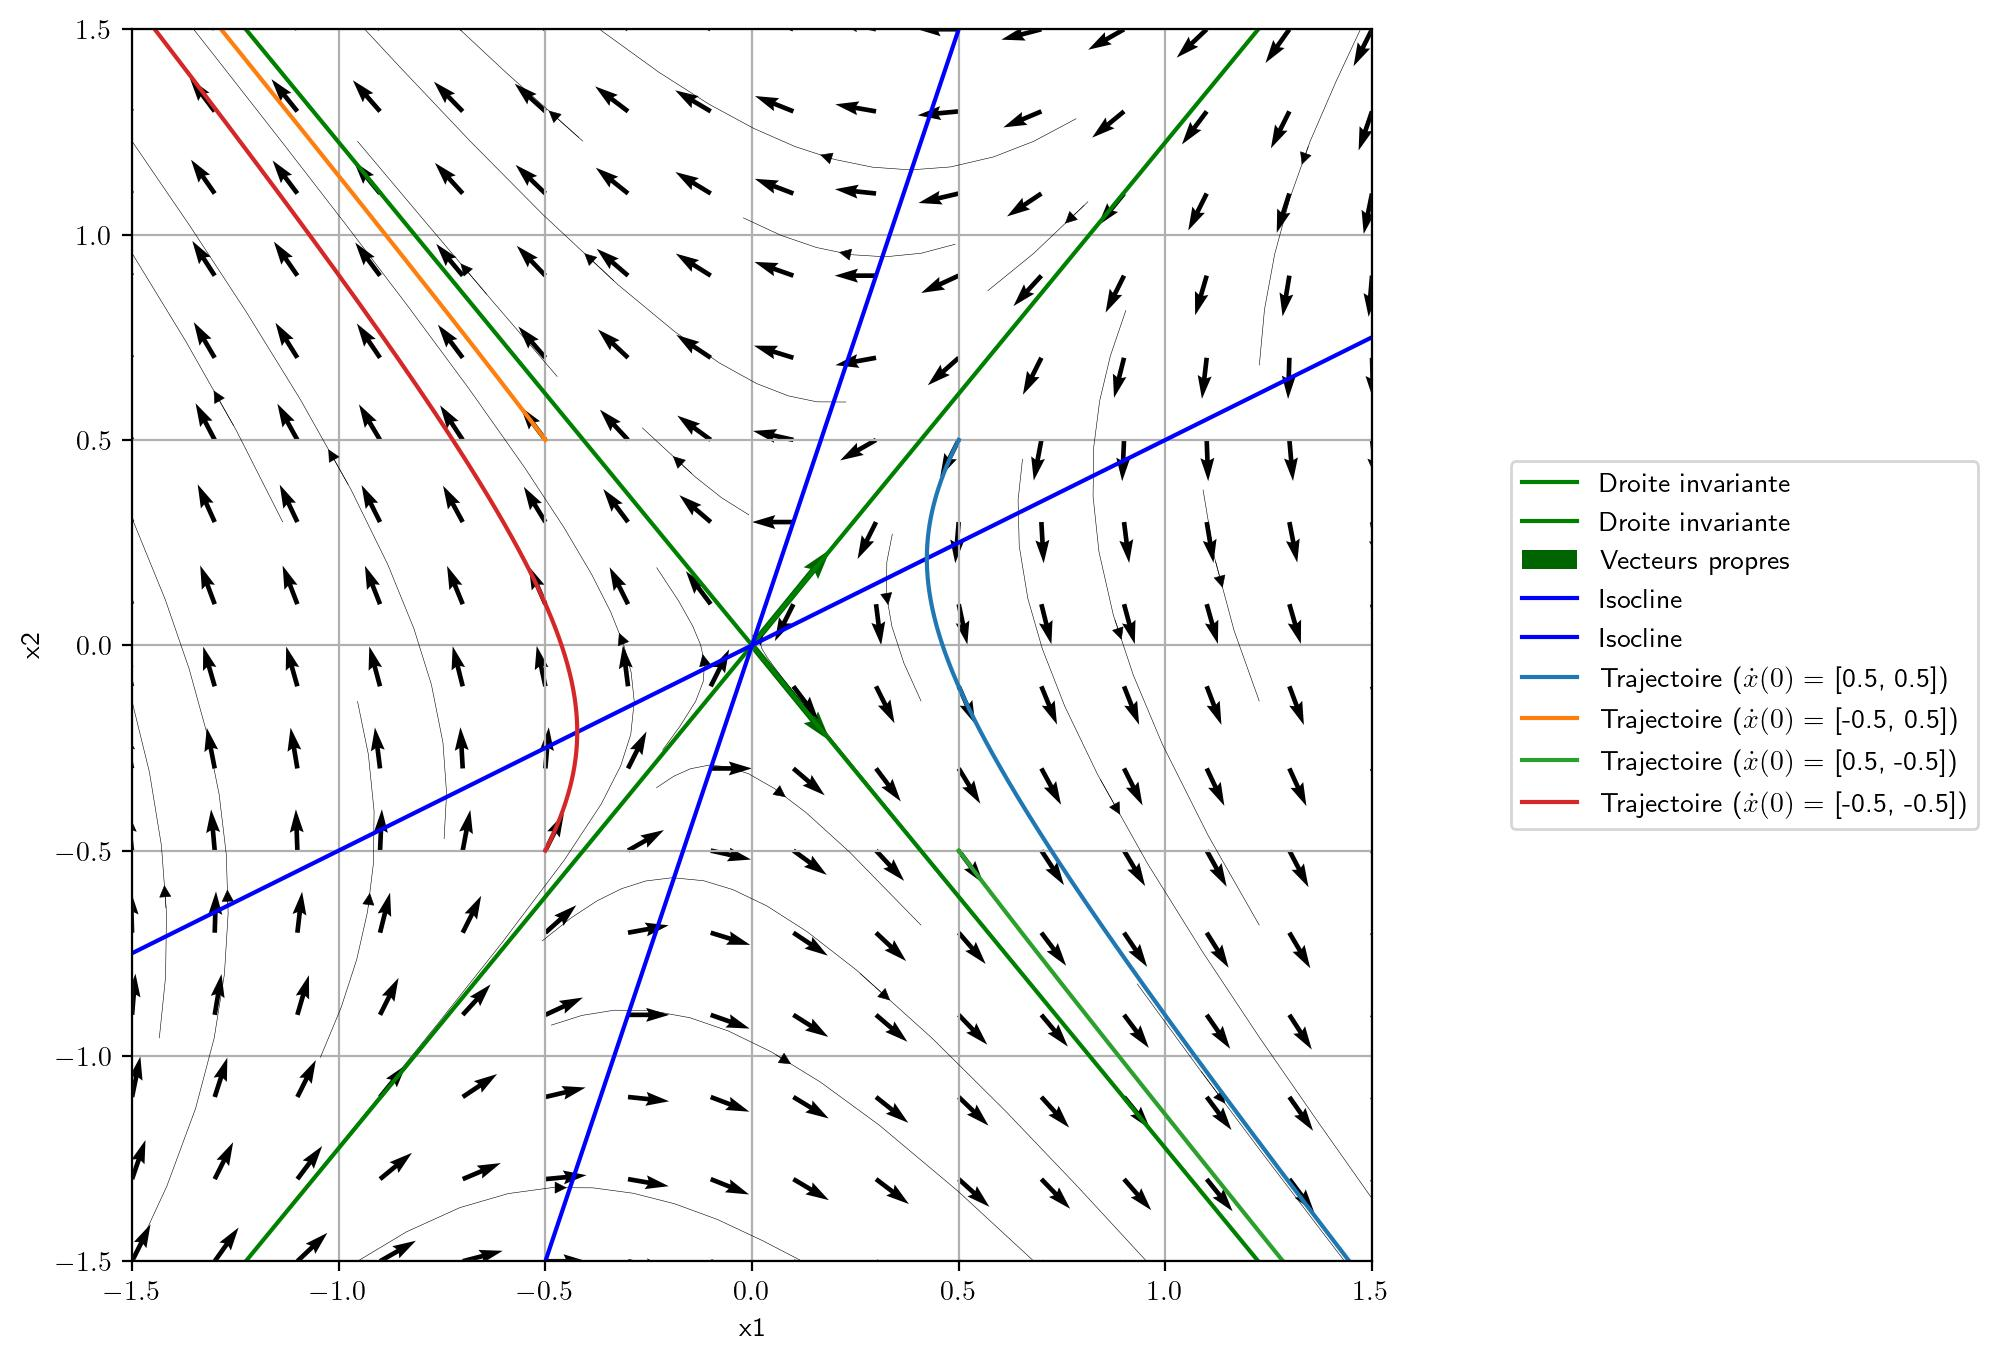
\includegraphics[width=\textwidth]{images/exemple_portrait_de_phases.jpg}
            \caption{Exemple de portrait de phases}
            \label{fig:exemple_portrait_de_phases}
        \end{figure}

        L'étude et le dessin des portraits de phases est un sujet autant complexe qu'il existe une infinité de systèmes possibles. Dans ce chapitre, nous nous concentrerons sur les systèmes d'équations différentielles d'ordre 2. Nous commençons par présenter de manière extensive les cas envisageables, en montrant les méthodes de résolutions et en amenant des cas par des exercices à réaliser sur papier. Dans la suite du chapitre, à la section \ref{sec:poincare}, nous présenterons la relation entre tous les comportements du système et la localisation de ce système dans le \textit{diagramme de Poincaré}, ce qui permettra d'accélérer nettement l'évaluation du comportement du système. 

        Nous pensons qu'il est indispensable de construire une intuition du comportement des systèmes autour des points d'équilibre pour bien comprendre, et non pas retenir, la construction de ce diagramme de Poincaré. La confrontation aux exemples avant la présentation d'une méthode plus générale conviendra aux étudiant·e·s qui préfèrent généraliser par l'exemple. Sinon, la section \ref{sec:poincare} présente ce diagramme, et peut être abordé avant d'étudier chaque cas individuellement. Nous insistons néanmoins sur la nécessité d'étudier chaque type de comportement individuellement, car chacun a ses subtilités de calcul qui doivent être explorées.
    
    \section{Points d'équilibre et stabilité}
        \begin{definition}{Point d'équilibre}
            Un point d'équilibre (ou \textit{point fixe}) est un point à partir duquel la trajectoire coïncide avec la condition initiale.
        \end{definition}
         Il répond à la condition $\dot{x} = 0$, étant donné que sa variation doit être nulle. Si $A$ est la matrice des coefficients du système étudié, et que $\det(A) \neq 0$, alors le seul état d'équilibre est $(0, 0)$. \robin{La caractérisation des solutions aux systèmes linéaires a été vue en F205, ça doit donc être connu ici} Sinon, il en existe d'autres.
         Une fois le(s) point(s) d'équilibre déterminés, on peut étudier la notion de stabilité. Comme vu au cours théorique, on dit qu'une trajectoire est \textit{stable} selon le critère de Liapounov si, pour tout point initial proche de cette trajectoire, les trajectoires qui en résultent restent dans un voisinage suffisamment petit autour de l'orbite au fil du temps. Autrement dit, si l'on perturbe légèrement un point sur cette orbite, la trajectoire de ce point perturbé restera à proximité de l'orbite initiale au lieu de s'en écarter indéfiniment. 

        \begin{definition}{Système stable}
            Un système dynamique linéaire est dit \textbf{stable} si son mouvement libre est limité pour chaque valeur de la condition initiale.
        \end{definition}

        \begin{definition}{Système asymptotiquement stable}
            Un système dynamique linéaire est dit \textbf{asymptotiquement stable} si son mouvement libre tend vers le point d'équilibre pour $t \to \infty$ pour chaque valeur de la condition initiale.
        \end{definition}

        \begin{definition}{Système instable}
            Un système dynamique linéaire est dit \textbf{instable} s'il existe au moins une condition initiale telle que le mouvement libre qui en suit est non limité.
        \end{definition}

        On peut distinguer des cas plus précis, qui dépendent du type et du signe des valeurs propres du système que l'on regarde. 
        Si les deux valeurs propres sont réelles et négatives, l'état d'équilibre est stable et est appelé un \textit{nœud stable}. Si les deux valeurs propres sont réelles et positives, l'état d'équilibre est instable et est appelé un \textit{nœud instable}. Si l'une est positive et l'autre négative, l'état d'équilibre est instable et est appelé une \textit{selle}. Ces différents cas seront présentés plus en détail.

    
    \section{Les vecteurs vitesse}
        Soit le système
        \begin{equation}
            \dot{x} = A x
        \end{equation}
        avec 
        \begin{equation}
            A = \begin{bmatrix} -2 & 1 \\ 1 & -2 \end{bmatrix}
        \end{equation}
        Soit un instant $t$ tel que l'état $x = \begin{bmatrix} 0.5 \\ 0 \end{bmatrix}$. Le vecteur vitesse à cet état est défini en résolvant le système d'équations différentielles \robin{Ce n'est pas un système d'équations différentielles~: $t$ est fixé, on cherche juste à résoudre un système linéaire dans $\mathbb R$}, par
        \begin{equation}
            \begin{bmatrix} \dot{x}_1 \\ \dot{x}_2 \end{bmatrix} = A \begin{bmatrix} 0.5 \\ 0 \end{bmatrix}
        \end{equation}
        Ce vecteur donne le sens, la direction et la vitesse de la trajectoire à notre état $\begin{bmatrix}x_1\\ x_2\end{bmatrix}$. Calculons le vecteur vitesse :
        \begin{equation}
            \begin{cases}
                \dot{x}_1 = -2x_1 + x_2 = -1\\
                \dot{x}_2 = x_1 - 2x_2 = 0.5
            \end{cases}
        \end{equation}
        Le vecteur vitesse est donc $\dot{x} = \begin{bmatrix} -1\\ 0.5\end{bmatrix} $.
        Calculons le vecteur vitesse au point $x = \begin{bmatrix} -0.5 \\ -1 \end{bmatrix}$ :
        \begin{equation}
            \begin{cases}
                \dot{x}_1 = -2x_1 + x_2 = 0 \\
                \dot{x}_2 = x_1 - 2x_2 = 1.5
            \end{cases}
        \end{equation}
        Le vecteur vitesse est donc $\dot{x} = \begin{bmatrix} 0\\ 1.5\end{bmatrix} $. 
        Avec cette méthode, on peut déterminer le vecteur vitesse en tout point du plan \robin{de l'espace des phases. Ici c'est un plan, mais ça fonctionne conceptuellement en dimension arbitraire}. 
        
        Si l'on trace les vecteurs vitesse pour un ensemble suffisamment grand de points, on obtient une première estimation du comportement du système, comme montré dans la figure \ref{fig:vecteurs_vitesse} pour le système décrit par la matrice 
        \begin{equation}
            A = \begin{bmatrix}1 & -2\\-2 & 1\end{bmatrix}
        \end{equation}
        Cette visualisation peut être obtenue grâce au code python suivant :
        \inputminted{python}{codes/vecteurs_vitesse.py}
        
        \begin{figure}[ht!]
            \centering
            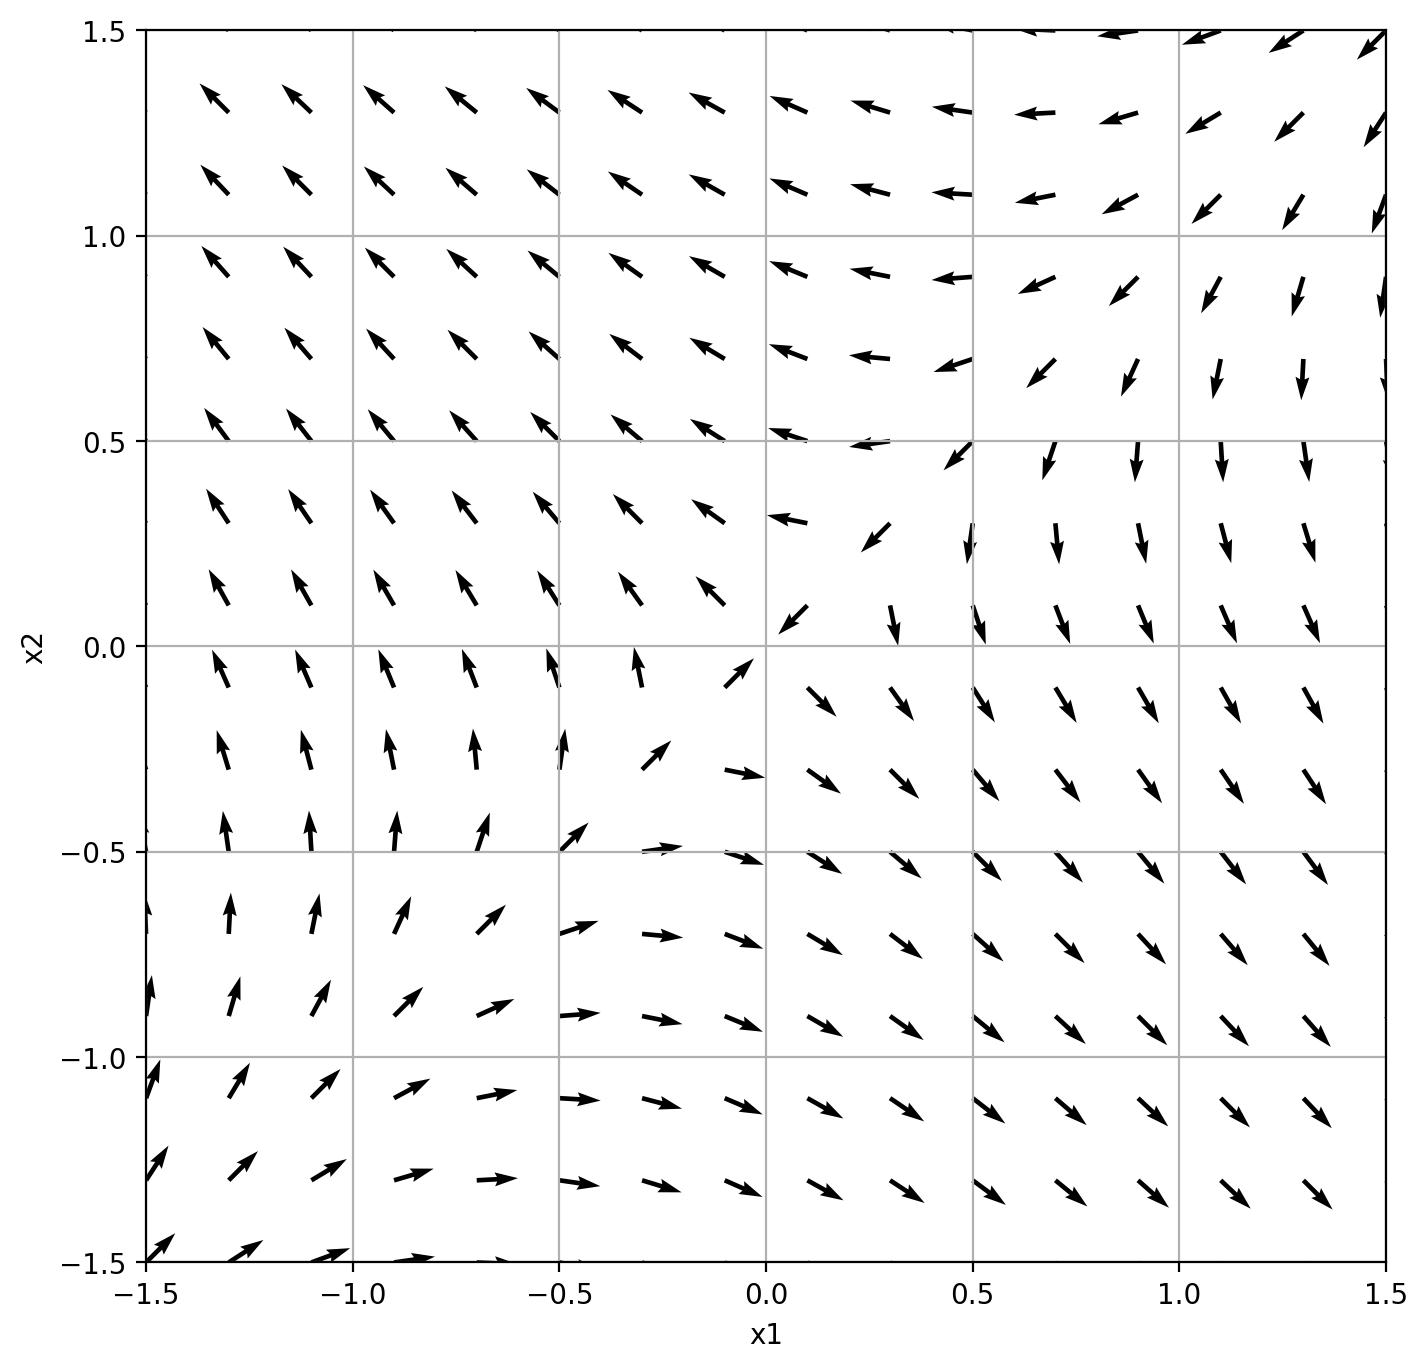
\includegraphics[width=\textwidth]{images/vecteurs_vitesse.jpg}
            \caption{Exemple de vecteurs vitesse}
            \label{fig:vecteurs_vitesse}
        \end{figure}

    
    \section{Valeurs propres et vecteurs propres}
        Calculons les valeurs propres du système décrit par $A$:
        \begin{equation}
            \begin{split}
            \det(A - \lambda I) &= 0 \\
            \Rightarrow \lambda^2 + 4\lambda + 3 &= 0\\
            \lambda_{1,2} = -4 \pm \sqrt{4} &= \{-1, -3\}
            \end{split}
        \end{equation}
        Calculons ses vecteurs propres :
        \begin{equation}
            \begin{split}
                &(A - \lambda_1 I)\overrightarrow{v_1} = 0 \\
                \Rightarrow& \begin{bmatrix} -1 & 1 \\ 1 & -1 \end{bmatrix} \begin{bmatrix} x \\ y \end{bmatrix} = \begin{bmatrix} 0 \\ 0 \end{bmatrix}\\
                \Rightarrow& \begin{bmatrix} x \\ y \end{bmatrix} = k \cdot \begin{bmatrix} 1 \\ 1 \end{bmatrix} \quad \forall k \\
                \Rightarrow& \overrightarrow{v_1} = \begin{bmatrix} 1 \\ 1 \end{bmatrix}
            \end{split}
        \end{equation}
        et pour $\lambda_2$,
        \begin{equation}
            \begin{split}
                &(A - \lambda_2 I)\overrightarrow{v_2} = 0 \Rightarrow \begin{bmatrix} 1 & 1 \\ 1 & 1 \end{bmatrix} \begin{bmatrix} x \\ y \end{bmatrix} = \begin{bmatrix} 0 \\ 0 \end{bmatrix}\\
                \Rightarrow& \begin{bmatrix} x \\ y \end{bmatrix} = k \cdot \begin{bmatrix} 1 \\ -1 \end{bmatrix} \quad \forall k \\
                \Rightarrow& \overrightarrow{v_2} = \begin{bmatrix} 1 \\ -1 \end{bmatrix}
            \end{split}
        \end{equation}

        De nouveau, il est possible de calculer ces vecteurs propres numériquement en python, grâce au code suivant:
        \inputminted{python}{codes/vecteurs_propres.py}
        Et le résultat peut être affiché comme montré dans la figure \ref{fig:vecteurs_propres}.
        \begin{figure}[ht!]
            \centering
            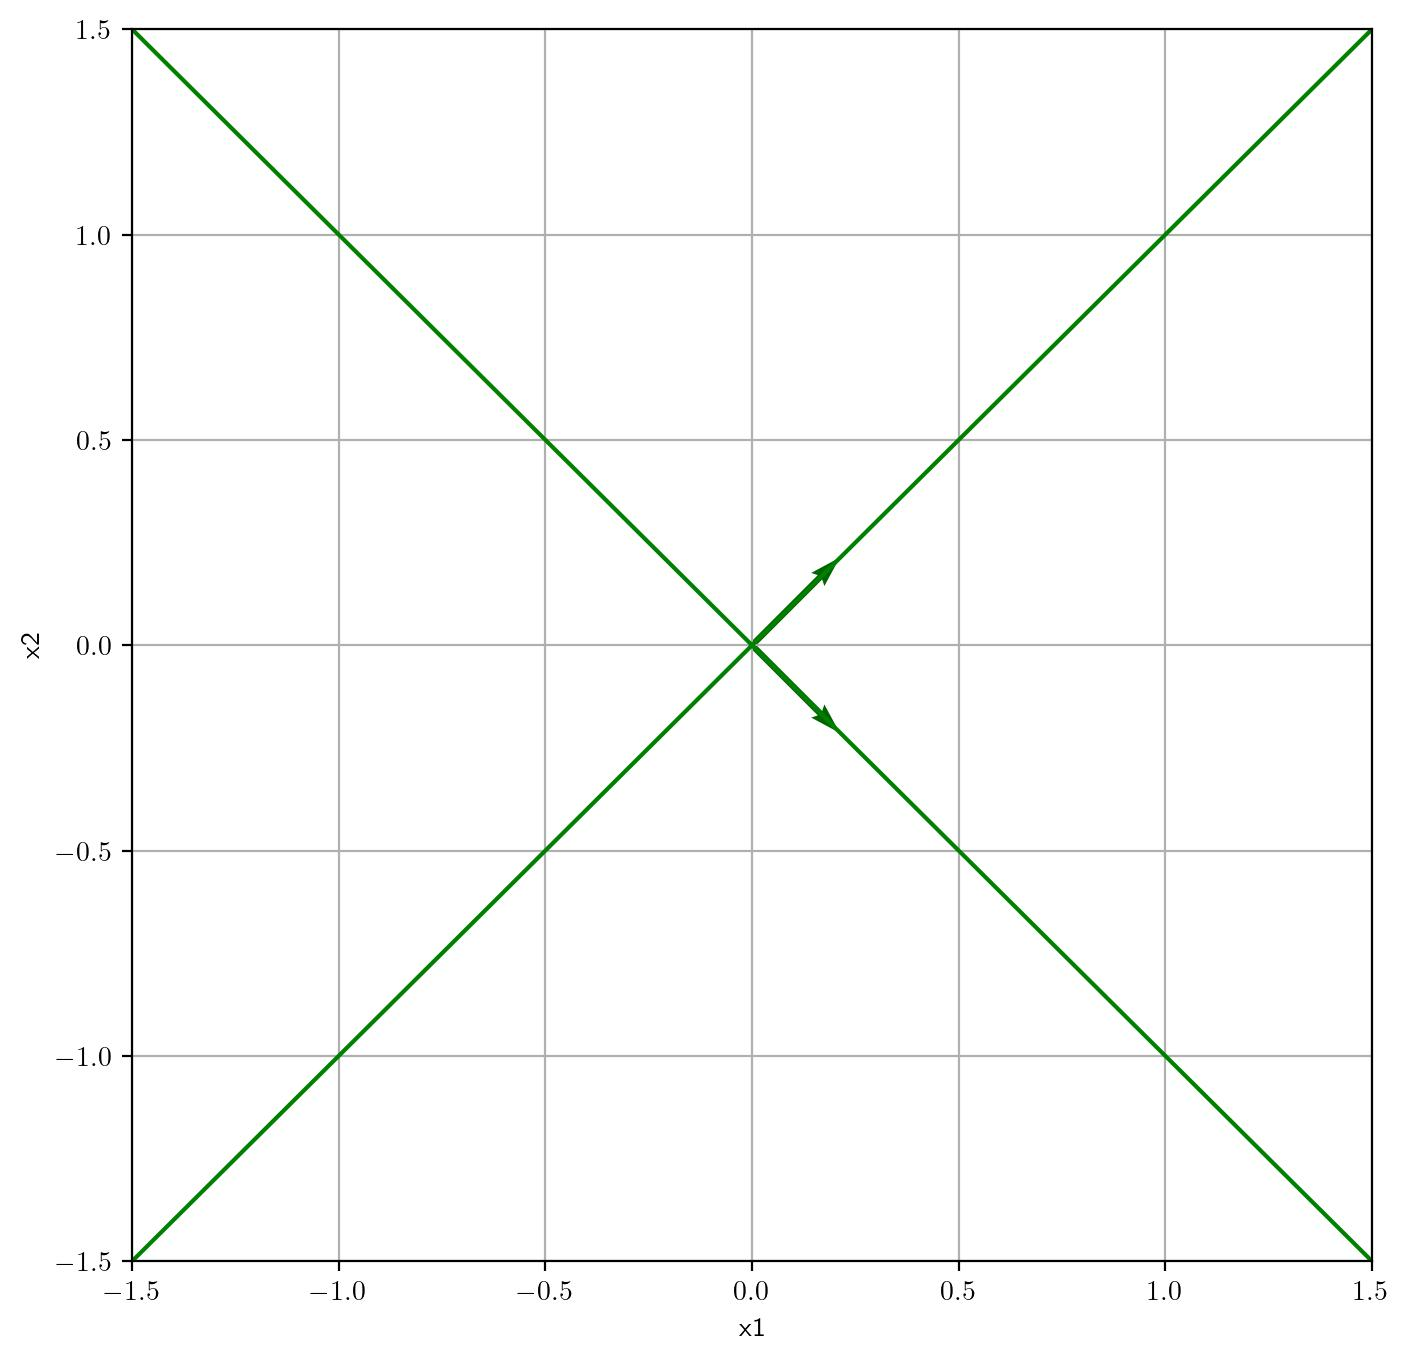
\includegraphics[width=\textwidth]{images/vecteurs_propres.jpg}
            \caption{Exemple de vecteurs vitesse \robin{Ce sont les vecteurs propres ici, pas les vecteurs vitesse}}
            \label{fig:vecteurs_propres}
        \end{figure}
        
        Notez bien que tout vecteur qui est un multiple de l'un des vecteurs propres que nous avons calculés est encore un vecteur propre.
        Prenons un état correspondant à un multiple du vecteur propre $\overrightarrow{v_1} = \begin{bmatrix} 1 \\ 1 \end{bmatrix}$, par exemple $\begin{bmatrix}2\\ 2\end{bmatrix}$, et calculons son vecteur vitesse :
        \begin{equation}
            \begin{cases}
                \dot{x}_1 = -2x_1 + x_2 = -2 \\
                \dot{x}_2 = x_1 - 2x_2 = -2
            \end{cases}
        \end{equation}
        Le vecteur vitesse est donc $\begin{bmatrix}-2\\ -2\end{bmatrix}$. Notez que le déplacement reste dans la même direction que notre vecteur vitesse initial.

        En règle générale : si on part d'un état $v$ qui est un multiple d'un vecteur propre, le vecteur vitesse a la même direction que ce vecteur propre.
        
        Cette règle est vérifiable formellement. Soit une paire de vecteur et valeur propre $(v, \lambda)$. Nous avons par définition
        \begin{equation}
            A v = \lambda v
        \end{equation}
        et donc, en revenant au système, si on part d'un état $x = k \cdot v$, nous avons
        \begin{equation}
            \begin{split}
                &\dot{x} = A x \\
                \Rightarrow& \dot{x} = k A v = k \lambda v
            \end{split}
        \end{equation}
        Nous voyons donc que le vecteur vitesse $\dot{x}$ est bien un multiple du vecteur propre $v$.
    \section{Exercices}
        Comme dans le chapitre sur la résolution d'équations différentielles, on vous donne un système d'équations différentielles d'ordre 2, de la forme \robin{Tu utilises $A_{ij}$ (en majuscule) alors que tu utilisais $a_{ij}$ dans le chapitre précédent}
        \begin{equation}
            \begin{cases}
                \dot{x}_1(t) = A_{00} x_1(t) + A_{01} x_2(t)\\
                \dot{x}_2(t) = A_{10} x_1(t) + A_{11} x_2(t)
            \end{cases}
        \end{equation}
        Vous devez:
        \begin{enumerate}
            \item définir la matrice des coefficients~;
            \item définir l'équation caractéristique~;
            \item calculer les valeurs propres~;
            \item déterminer les vecteurs propres, et les trajectoires associées~;
            \item dessiner les vecteurs vitesses pour des points bien choisis~;
            \item dessiner la trajectoire du système pour ces conditions initiales pour un intervalle de temps donné.
        \end{enumerate}
        Ces exercices sont à réaliser à la main, sur papier millimétré. Afin d'offrir une auto-vérification, nous proposons les solutions générées par le code suivant:
        \inputminted{python}{codes/correction_pdp_1.py}
        
        \subsection{Exercice 1: nœud stable}
            \begin{exercise}{Nœud stable}
                Effectuez les étapes présentées à la section précédente pour le système
                \begin{equation}
                    \begin{cases}
                        \dot{x}_1(t) = x_1(t) - 2 x_2(t)\\
                        \dot{x}_2(t) = - 2 x_1(t) + x_2(t)
                    \end{cases}
                \end{equation}
            \end{exercise}
            Tracez les vecteurs vitesses en $x = \begin{bmatrix}1 \\ 1\end{bmatrix}$, $\begin{bmatrix}-1 \\ 1\end{bmatrix}$, $\begin{bmatrix}1 \\ -1\end{bmatrix}$ et $\begin{bmatrix}-1 \\ -1\end{bmatrix}$, et en $x = \begin{bmatrix}0 \\ 1\end{bmatrix}$, $\begin{bmatrix}1 \\ 0\end{bmatrix}$, $\begin{bmatrix}0 \\ -1\end{bmatrix}$ et $\begin{bmatrix}-0.5 \\ -1\end{bmatrix}$. Tracez les trajectoires démarrant en $x = \begin{bmatrix}0 \\ 1\end{bmatrix}$ et en $x = \begin{bmatrix}-0.5 \\ -1\end{bmatrix}$.
            La solution numérique est donnée en figure \ref{fig:pdp_exercice_1}.
            \begin{figure}[ht!]
                \centering
                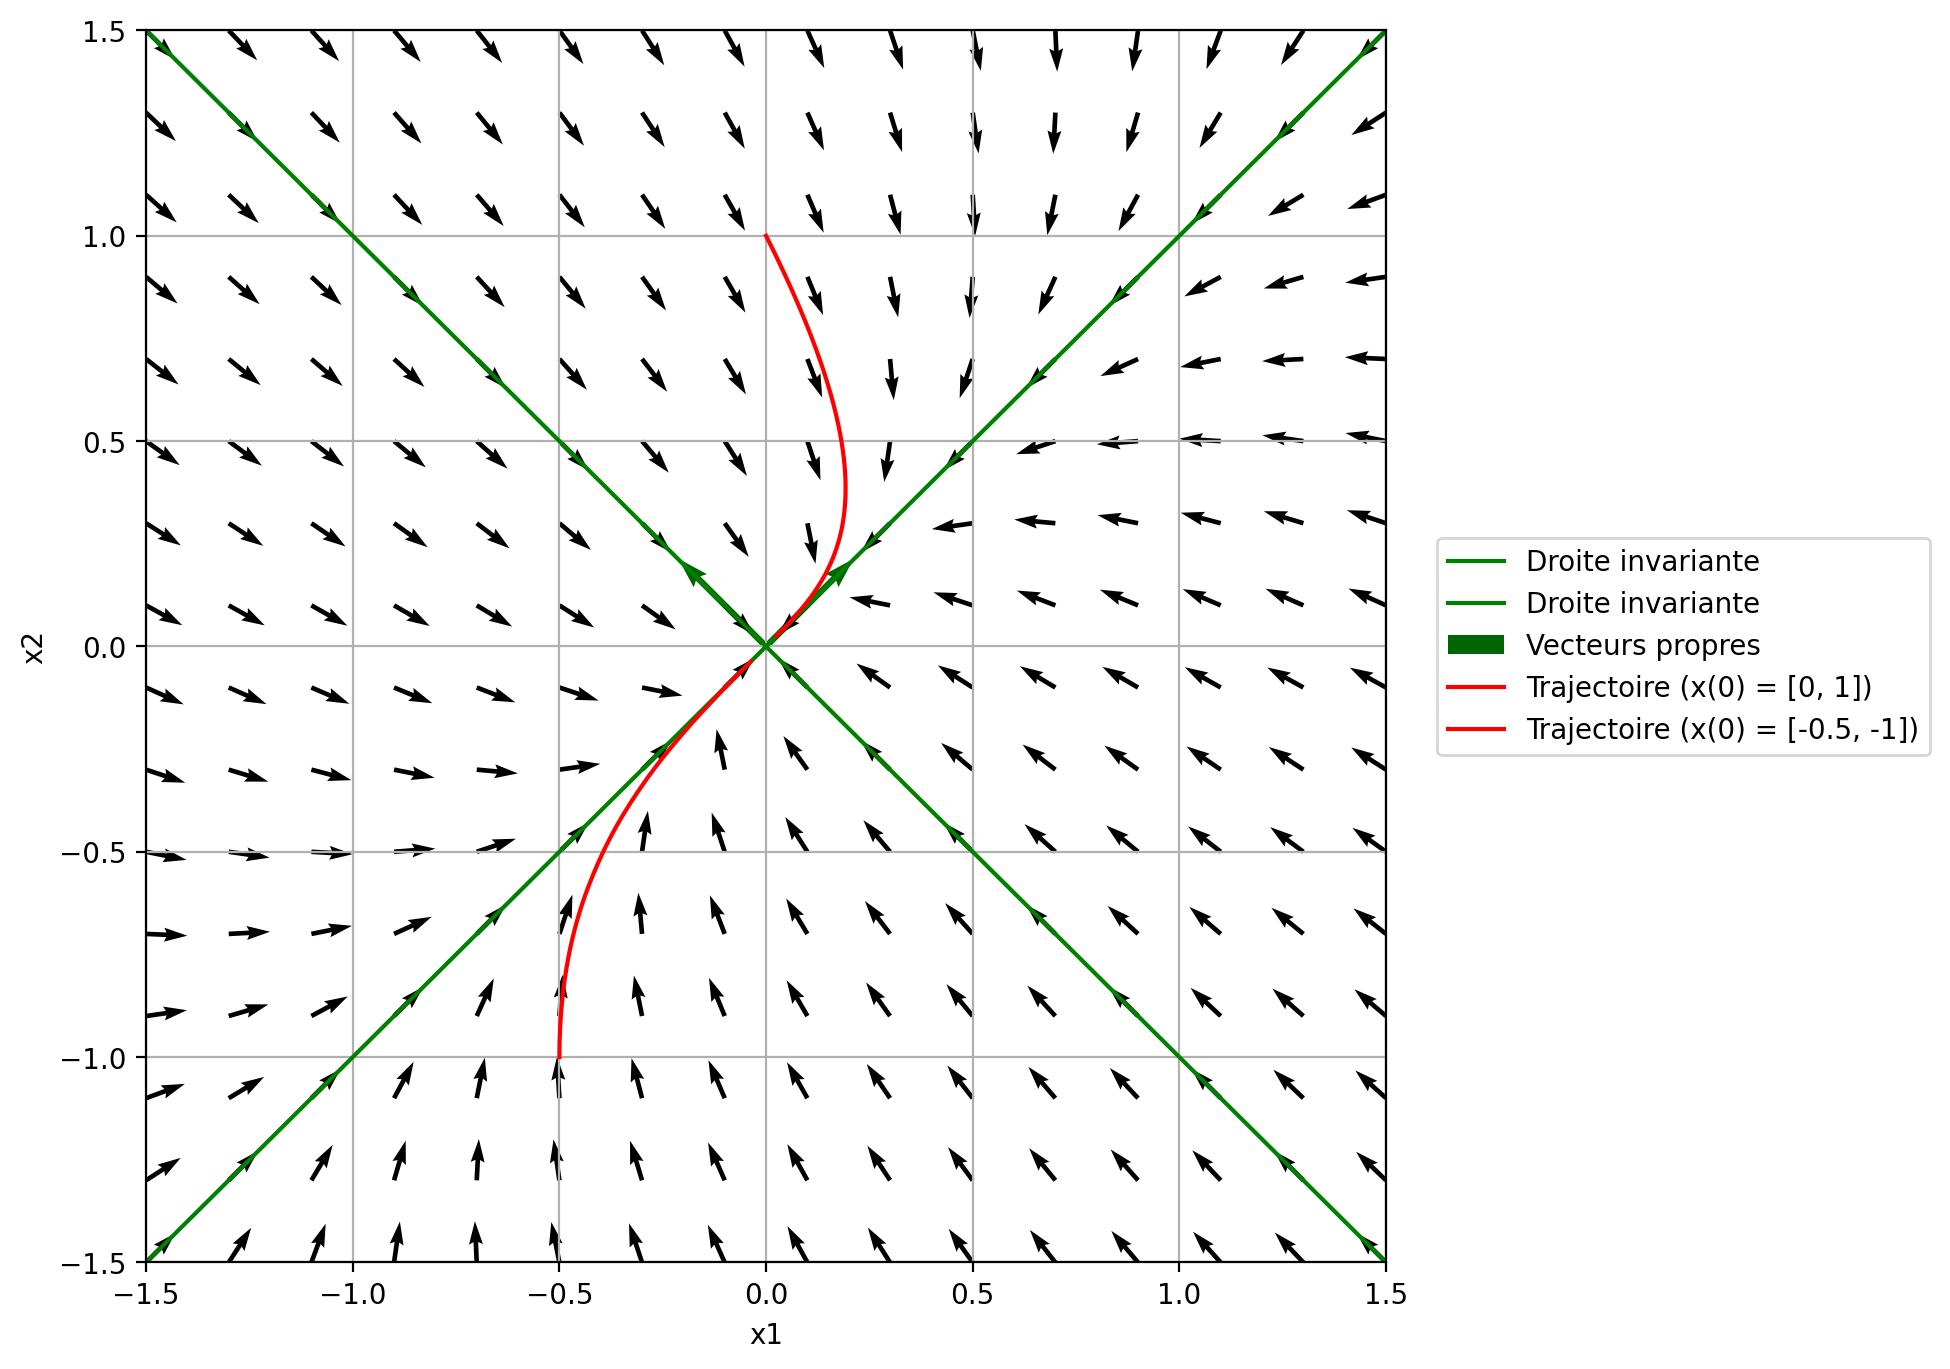
\includegraphics[width=\textwidth]{images/pdp_exercice_1.jpg}
                \caption{Solution numérique de l'exercice 1}
                \label{fig:pdp_exercice_1}
            \end{figure}
                
        \subsection{Exercice 2: nœud instable}
            \begin{exercise}{Nœud instable}
                Effectuez les étapes présentées à la section précédente pour le système
                \begin{equation}
                    \begin{cases}
                        \dot{x}_1(t) = 2 x_1(t) + x_2(t)\\
                        \dot{x}_2(t) = 2 x_1(t) + 3 x_2(t)
                    \end{cases}
                \end{equation}
            \end{exercise}
            Tracez les vecteurs vitesses en $x = \begin{bmatrix}0.5 \\ 1\end{bmatrix}$, $\begin{bmatrix}-0.5 \\ -1\end{bmatrix}$, $\begin{bmatrix}-1 \\ 1\end{bmatrix}$ et $\begin{bmatrix}1 \\ -1\end{bmatrix}$, et en $x = \begin{bmatrix}0 \\ 1\end{bmatrix}$, $\begin{bmatrix}1 \\ 0\end{bmatrix}$, $\begin{bmatrix}0 \\ -1\end{bmatrix}$ et $\begin{bmatrix}-0.5 \\ -1\end{bmatrix}$. Tracez les trajectoires démarrant en $x = \begin{bmatrix}0 \\ 1\end{bmatrix}$ et en $x = \begin{bmatrix}-0.5 \\ -1\end{bmatrix}$.
            La solution numérique est donnée en figure \ref{fig:pdp_exercice_2}.
            \begin{figure}[ht!]
                \centering
                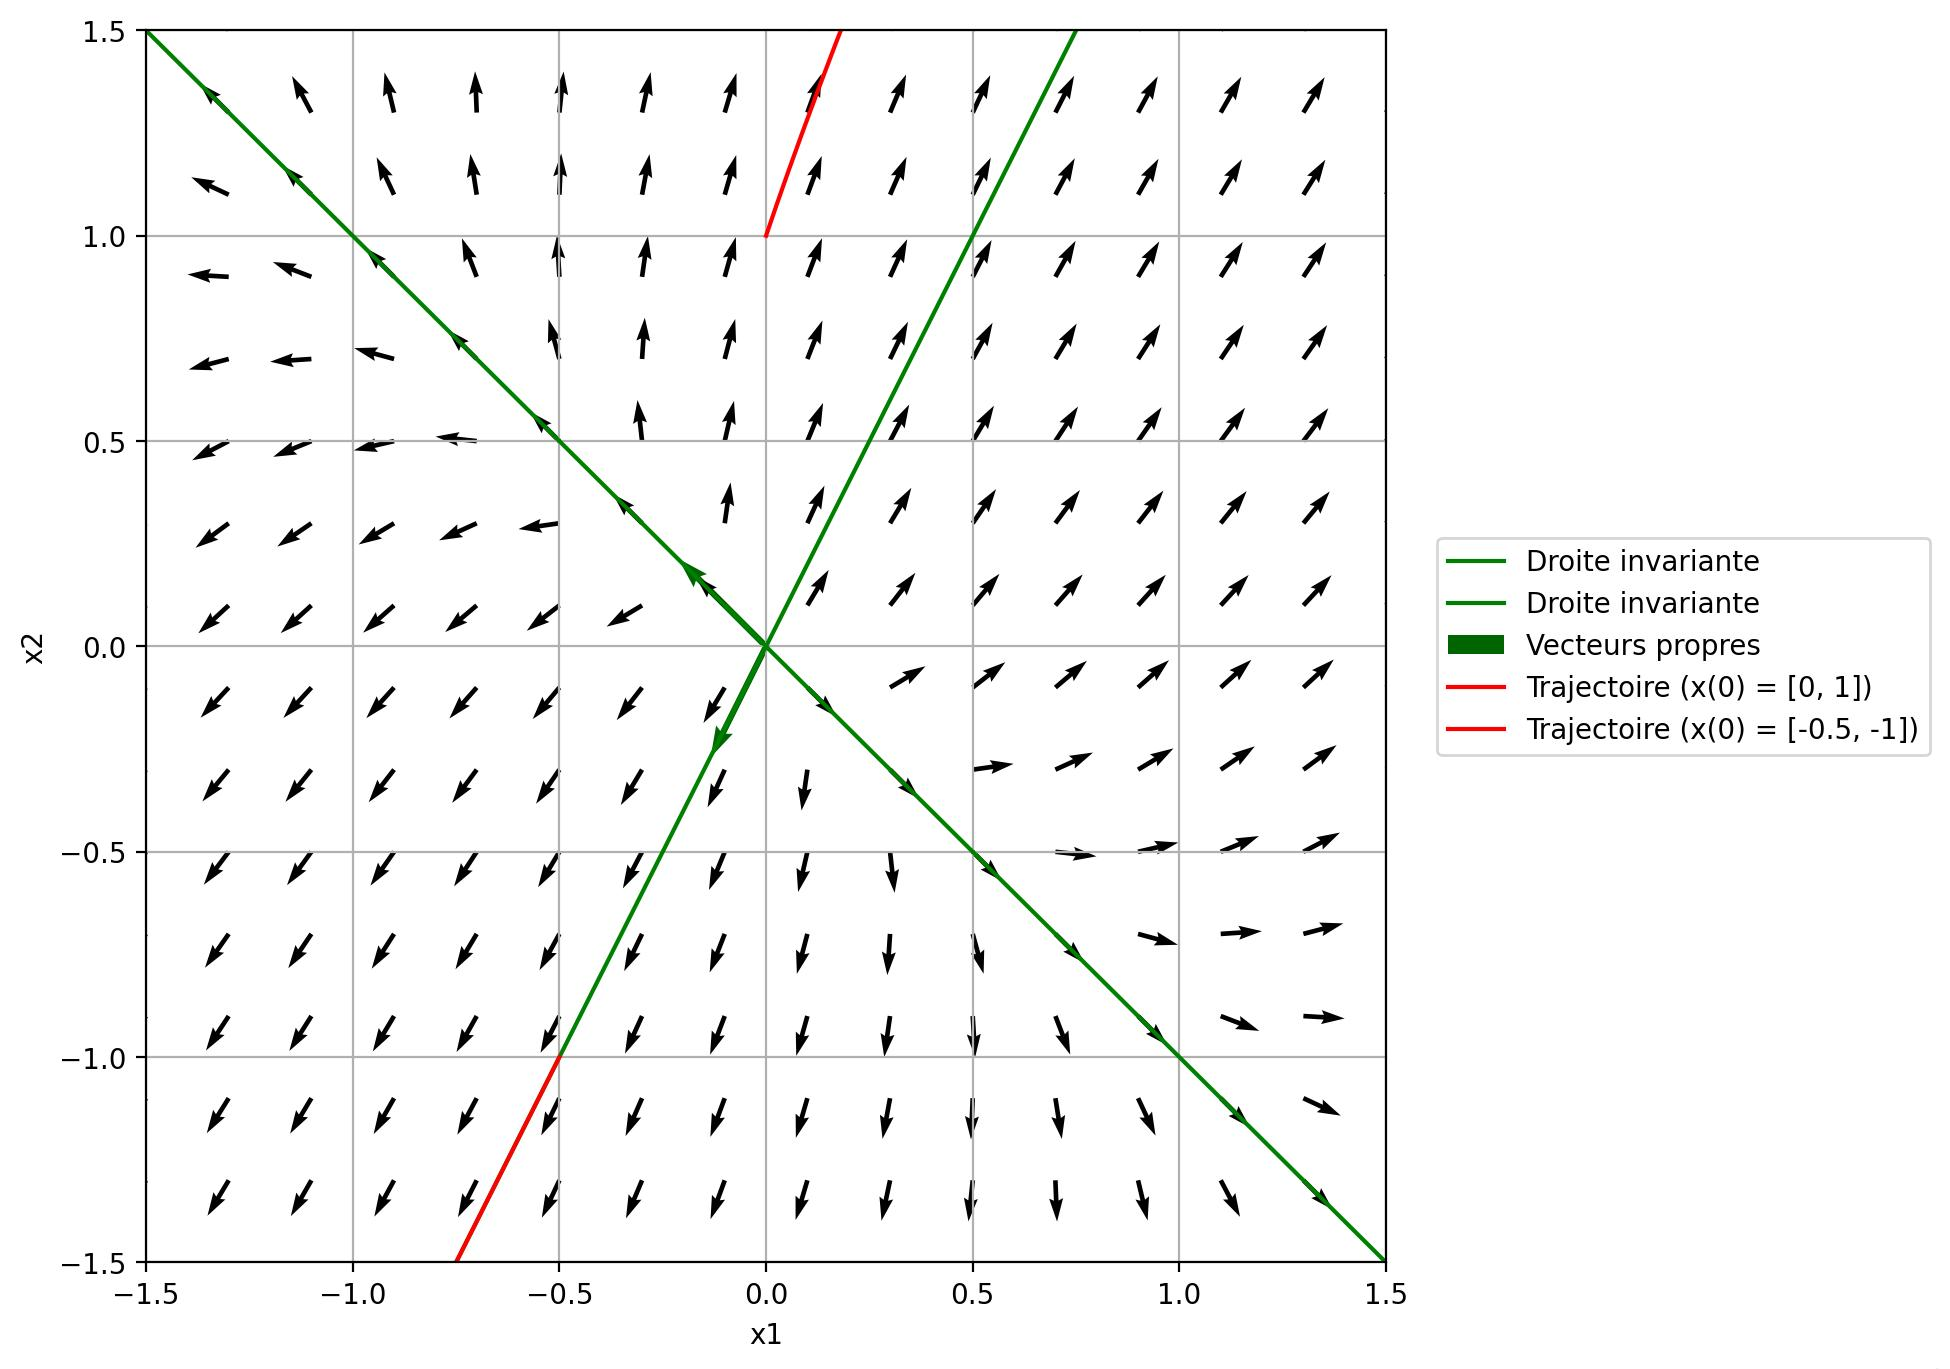
\includegraphics[width=\textwidth]{images/pdp_exercice_2.jpg}
                \caption{Solution numérique de l'exercice 2}
                \label{fig:pdp_exercice_2}
            \end{figure}
        
        \subsection{Exercice 3: selle}
            \begin{exercise}{Selle}
                Effectuez les étapes présentées à la section précédente pour le système
                \begin{equation}
                    \begin{cases}
                        \dot{x}_1(t) = 5 x_1(t) + 9 x_2(t)\\
                        \dot{x}_2(t) = 6 x_1(t) + 2 x_2(t)
                    \end{cases}
                \end{equation}
            \end{exercise}
            Tracez les vecteurs vitesses en $x = \begin{bmatrix}1 \\ \frac23\end{bmatrix}$, $\begin{bmatrix}-1 \\ -\frac23\end{bmatrix}$, $\begin{bmatrix}-1 \\ 1\end{bmatrix}$ et $\begin{bmatrix}1 \\ -1\end{bmatrix}$, et en $x = \begin{bmatrix}0 \\ 1\end{bmatrix}$, $\begin{bmatrix}1 \\ 0\end{bmatrix}$, $\begin{bmatrix}0 \\ -1\end{bmatrix}$ et $\begin{bmatrix}-0.5 \\ -1\end{bmatrix}$. Tracez les trajectoires démarrant en $x = \begin{bmatrix}0 \\ 1\end{bmatrix}$ et en $x = \begin{bmatrix}-0.5 \\ -1\end{bmatrix}$.
            La solution numérique est donnée en figure \ref{fig:pdp_exercice_3}.
            \begin{figure}[ht!]
                \centering
                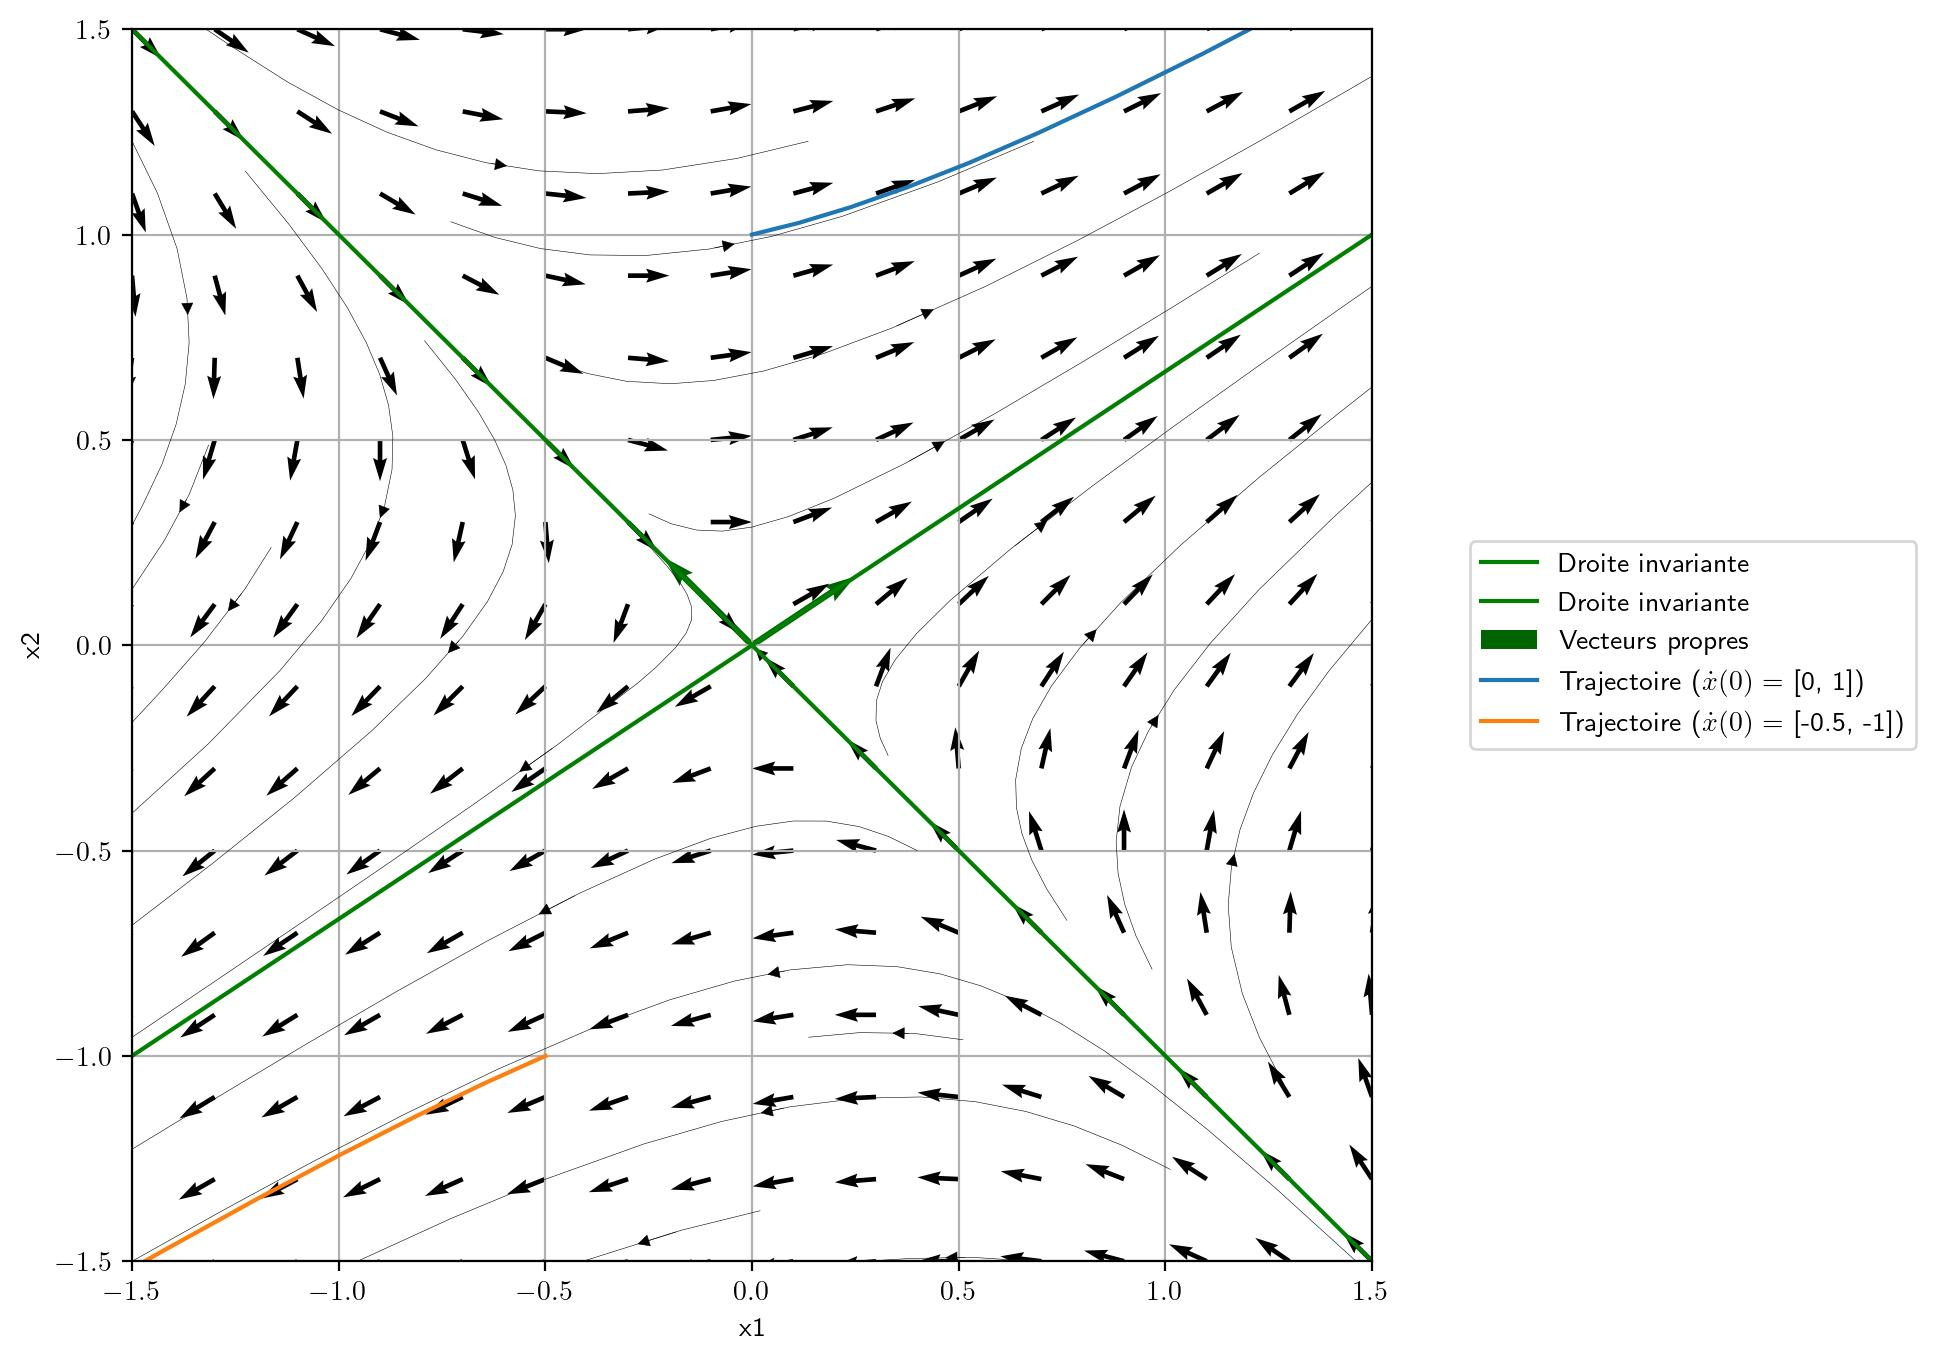
\includegraphics[width=\textwidth]{images/pdp_exercice_3.jpg}
                \caption{Solution numérique de l'exercice 3}
                \label{fig:pdp_exercice_3}
            \end{figure}
   \section{Systèmes non-simples}
        Dans cette section, nous étudions les portraits de phases des systèmes non-simples en analysant les différents types de valeurs propres et leurs implications sur la stabilité et les trajectoires dans le plan de phase. Nous considérons le système décrit par la matrice
        \begin{equation}
            A = \begin{bmatrix}
                a & b\\
                c & d
            \end{bmatrix}
        \end{equation}

        \subsection{Valeur propre nulle}
            Dans ce cas, où $\det A = 0$ avec $\lambda_1 = 0$, les états d'équilibre se trouvent sur la droite définie par :
            \begin{equation}
            ax_1 + bx_2 = 0,
            \end{equation}
            et les trajectoires suivent des droites parallèles dans la direction du vecteur propre associé $\mathbf{v}_2$. \robin{Notation de vecteur en gras alors que notation $\overrightarrow \cdot$ dans le chapitre précédent.} On distingue deux cas selon le signe de $\lambda_2$ :
            
            \begin{itemize}
                \item \textbf{Si $\lambda_2 < 0$ :} Les états d'équilibre sont stables, car toutes les trajectoires convergent vers la droite d'équilibre. \\
                \textit{Exemple :} $\lambda_1 = 0$, $\lambda_2 = -1$.
                
                \item \textbf{Si $\lambda_2 > 0$ :} Les états d'équilibre sont instables, car les trajectoires s'éloignent de la droite d'équilibre. \\
                \textit{Exemple :} $\lambda_1 = 0$, $\lambda_2 = 1$.
            \end{itemize}

        \subsection{Valeurs propres réelles et non-distinctes}
            Nous examinons ici le cas où $\lambda_1 = \lambda_2 = \lambda$, qui conduit à deux configurations selon la diagonalisabilité de $A$ :

            \begin{itemize}
                \item \textbf{Matrice $A$ diagonalisable :} Lorsque $A$ admet une infinité de vecteurs propres, chaque droite passant par l'origine est une trajectoire, et l'origine devient un \textit{nœud singulier}. Par exemple, le système décrit par la matrice
                \begin{equation}
                    A = \begin{bmatrix} -1 & 0 \\ 0 & -1 \end{bmatrix}
                \end{equation}
                décrit effectivement un nœud singulier, comme montré dans la figure \ref{fig:noeud_singulier}.
                \begin{figure}[ht!]
                    \centering
                    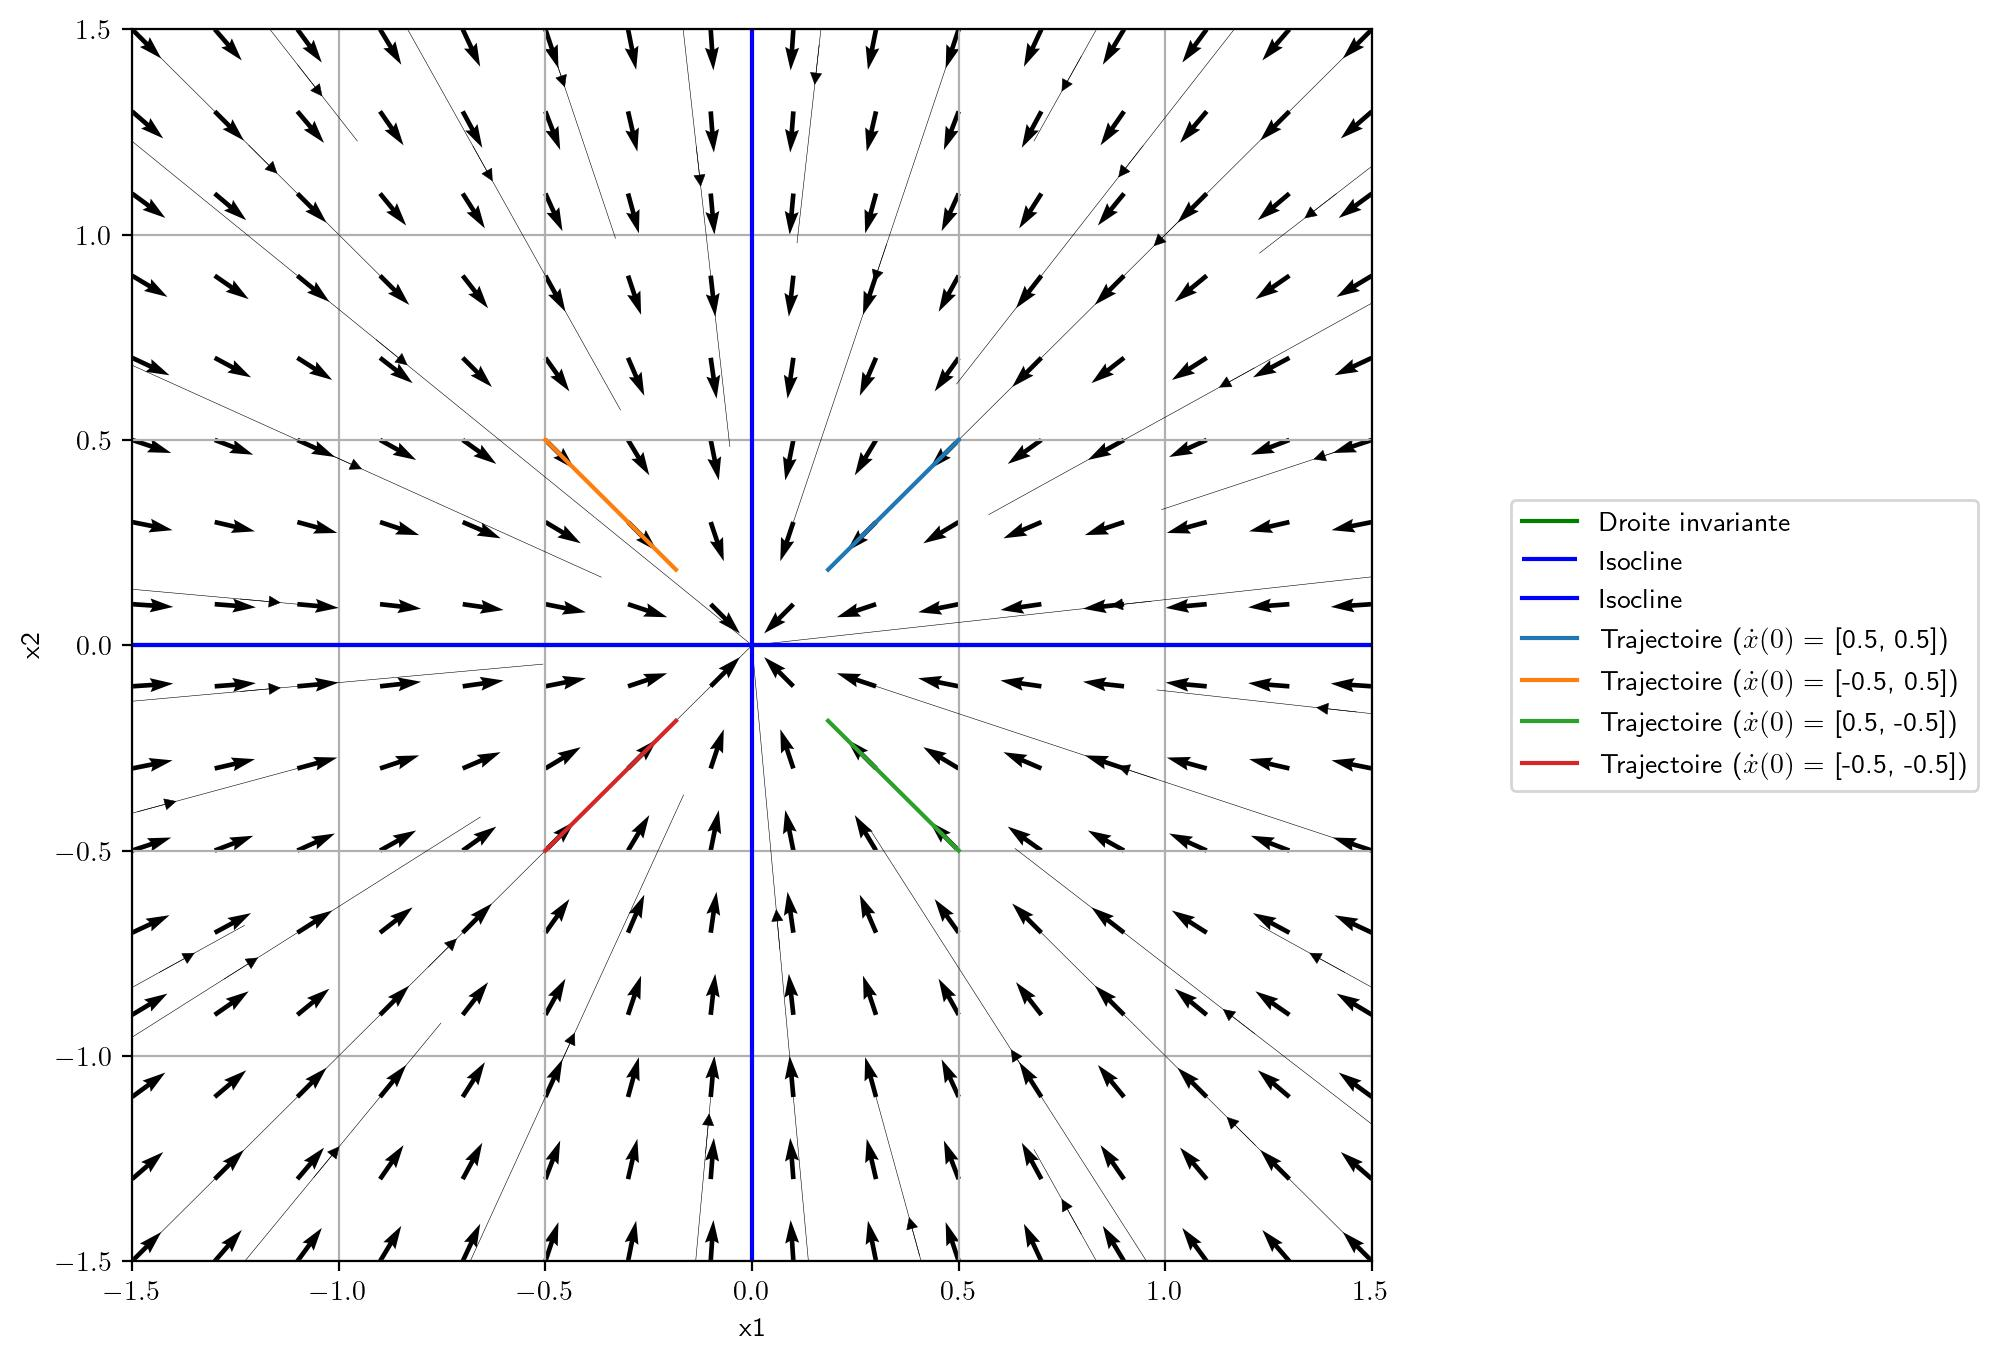
\includegraphics[width=\textwidth]{images/noeud_singulier.jpg}
                    \caption{Exemple de nœud singulier}
                    \label{fig:noeud_singulier}
                \end{figure}
                \begin{itemize}
                    \item Si $\lambda < 0$, le système est asymptotiquement stable.
                    \item Si $\lambda > 0$, le système est instable.
                    \item Si $\lambda = 0$, le système est simplement stable.
                \end{itemize}
            
                \item \textbf{Matrice $A$ non-diagonalisable :} Dans ce cas, $A$ n'a qu'un seul vecteur propre, et donc une seule direction possède une trajectoire rectiligne, tandis que les autres trajectoires prennent une forme parabolique. L'origine est alors un \textit{nœud dégénéré}. Par exemple, le système décrit par la matrice
                \begin{equation}
                    A = \begin{bmatrix} 3 & -4 \\ 1 & -1 \end{bmatrix}
                \end{equation}
                décrit effectivement un nœud dégénéré, comme montré dans la figure \ref{fig:noeud_degenere}.
                \begin{figure}[ht!]
                    \centering
                    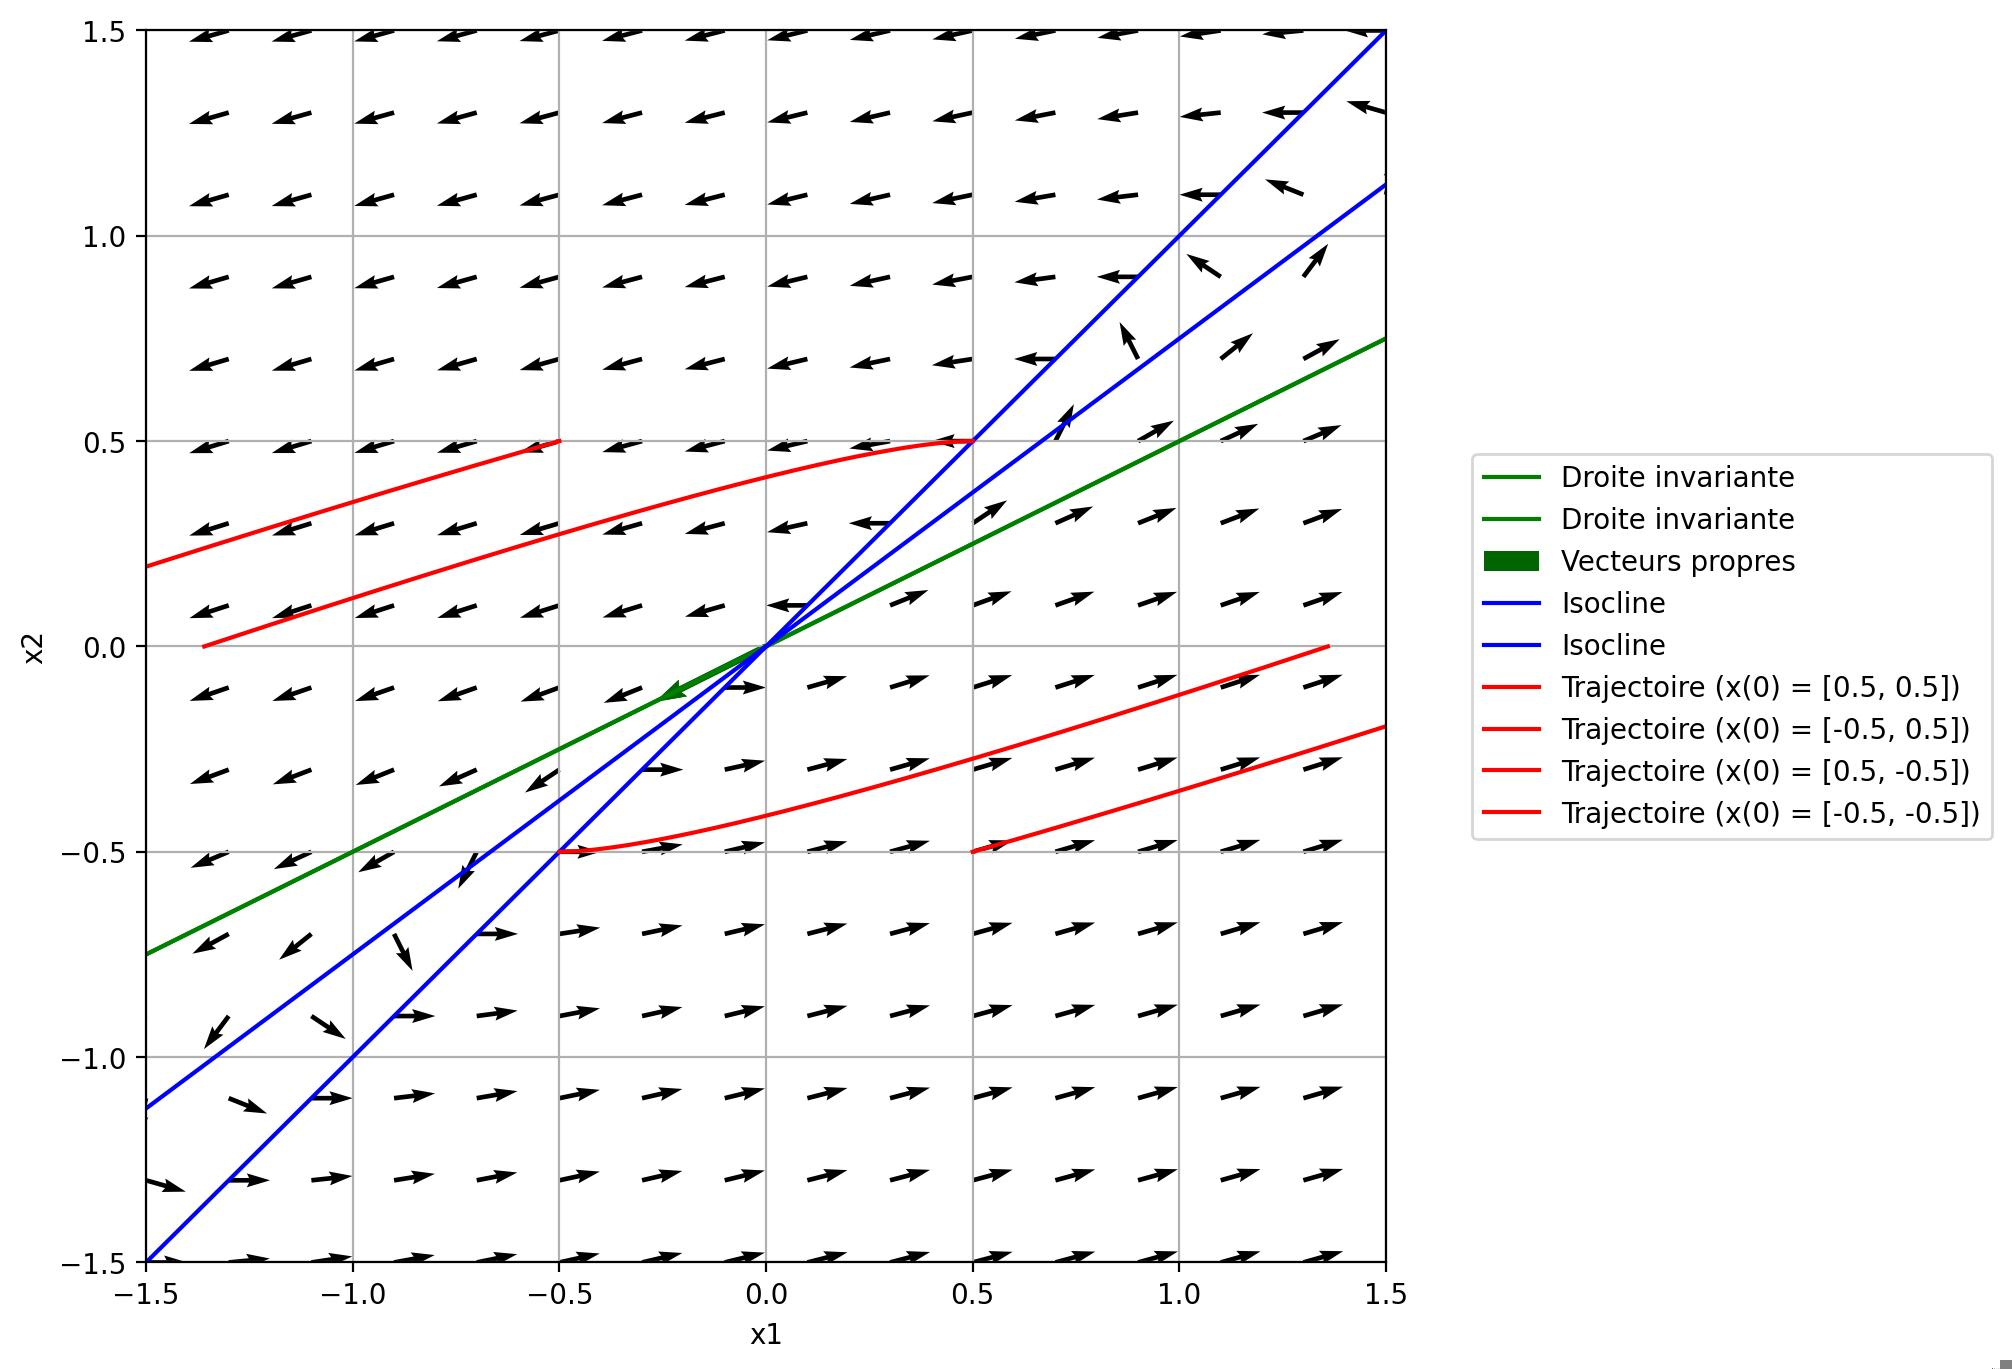
\includegraphics[width=\textwidth]{images/noeud_degenere.jpg}
                    \caption{Exemple de nœud dégénéré}
                    \label{fig:noeud_degenere}
                \end{figure}
                Si $\lambda = 0$, toutes les trajectoires se trouvent sur des droites parallèles, comme montré dans la figure \ref{fig:mouvement_uniforme} pour le système décrit par la matrice
                \begin{equation}
                    A = \begin{bmatrix} 1 & 0 \\ 1 & 0 \end{bmatrix}
                \end{equation}
                \begin{figure}[ht!]
                    \centering
                    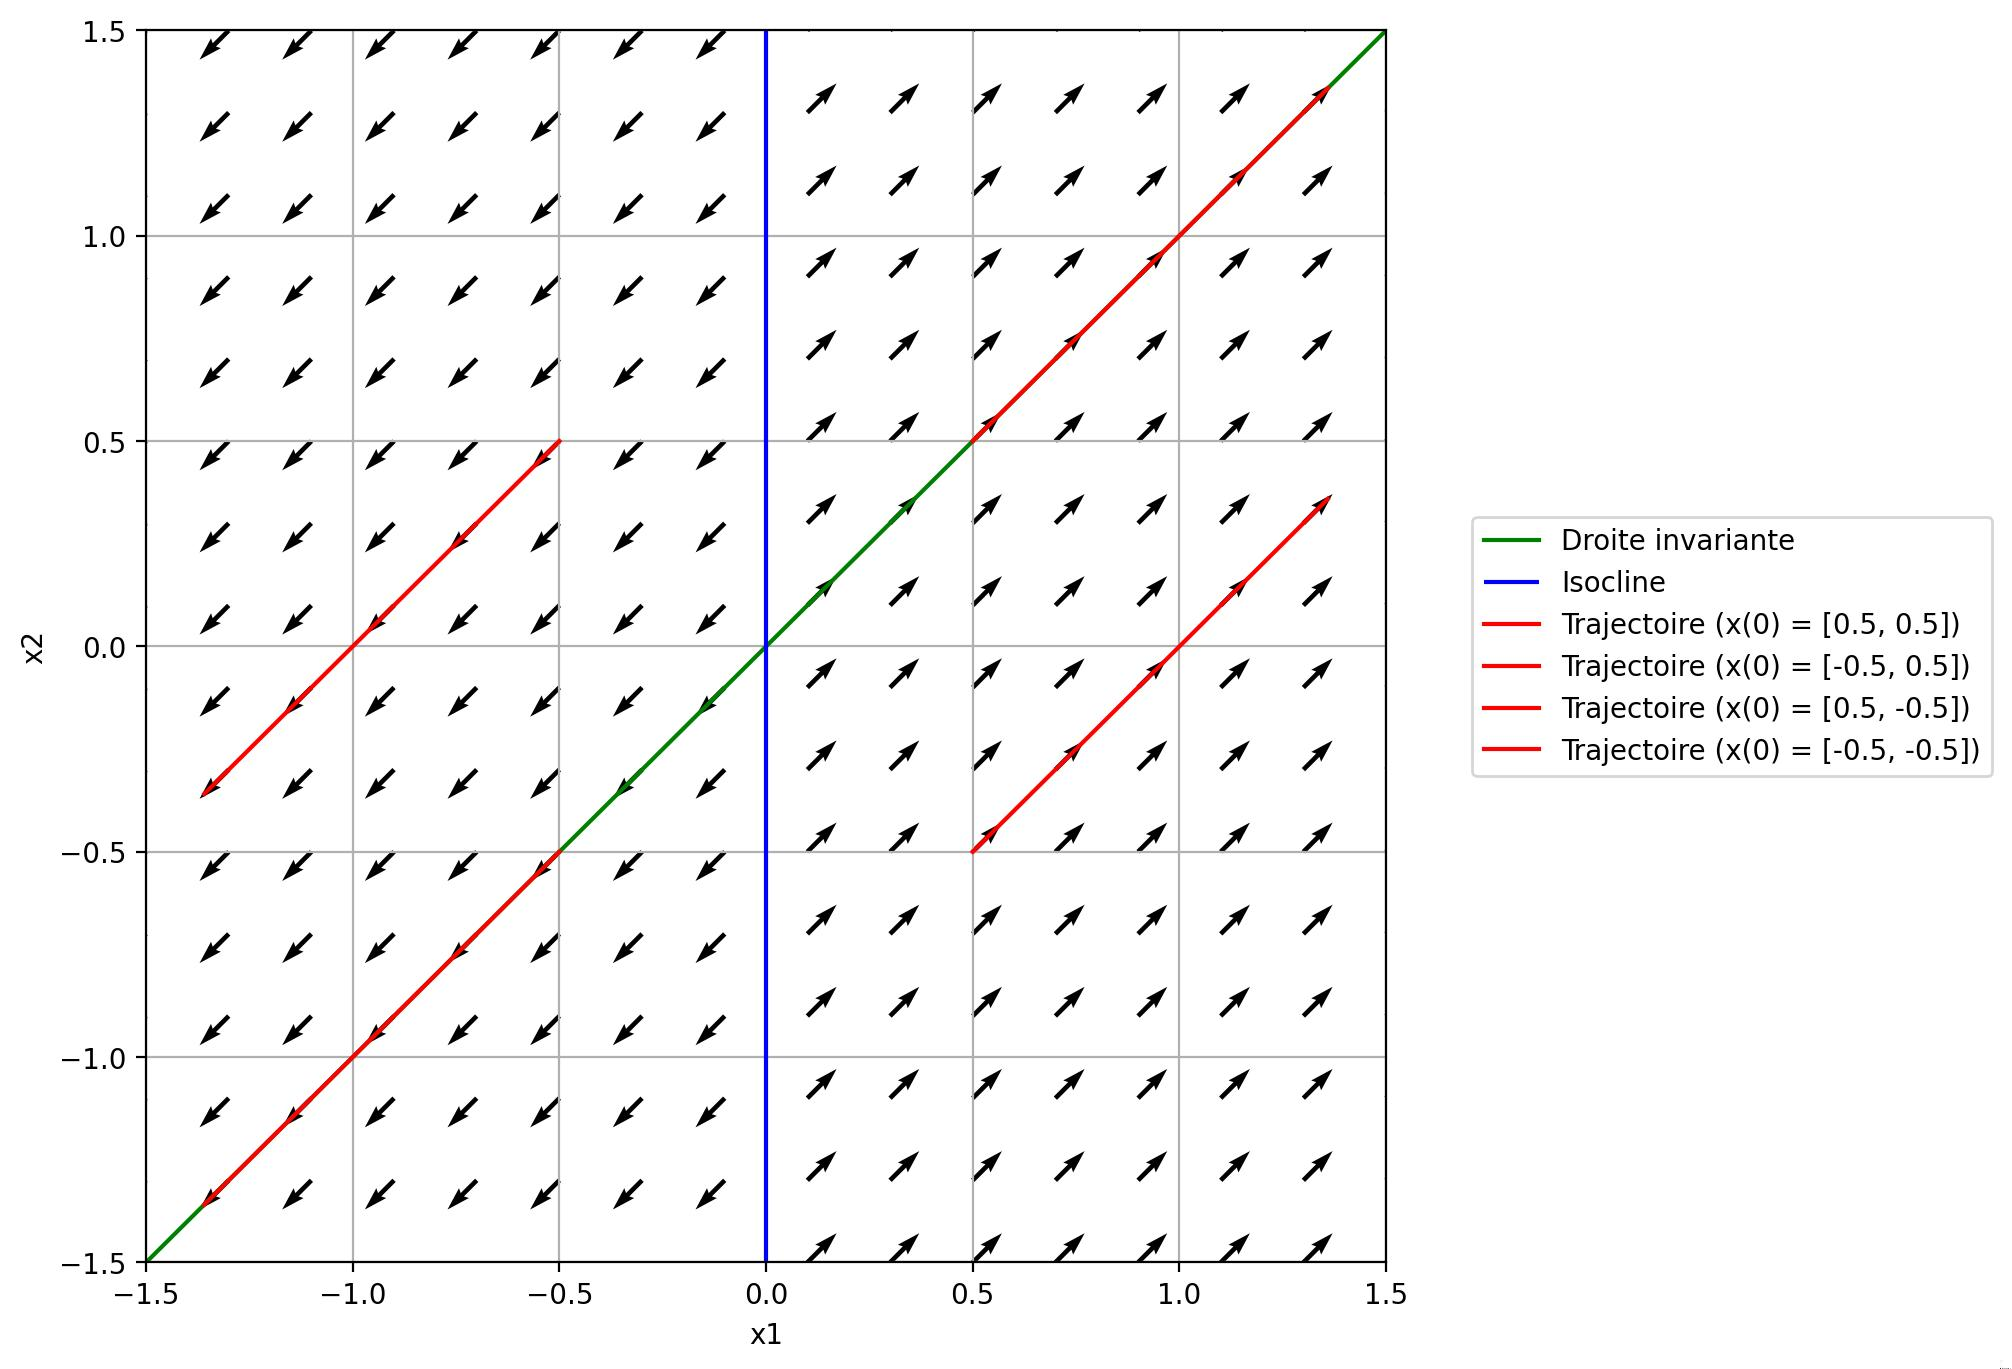
\includegraphics[width=\textwidth]{images/mouvement_uniforme.jpg}
                    \caption{Exemple de mouvement uniforme}
                    \label{fig:mouvement_uniforme}
                \end{figure}
            \end{itemize}

        \subsection{Valeurs propres complexes}
            Enfin, nous examinons le cas où les valeurs propres sont complexes : $\lambda_1 = a + ib$ et $\lambda_2 = a - ib$. Ici, la nature des trajectoires dépend du signe de la partie réelle $a$ :
            
            \begin{itemize}
                \item \textbf{Si $a = 0$ :} Les trajectoires forment des ellipses fermées avec une période de rotation $T = \frac{2 \pi}{|b|}$. L'origine est un \textit{centre}. Un exemple est montré en figure \ref{fig:centre}, avec la matrice
                \begin{equation}
                    A = \begin{bmatrix} 0 & 1 \\ -1 & 0 \end{bmatrix}
                \end{equation}
                \begin{figure}[ht!]
                    \centering
                    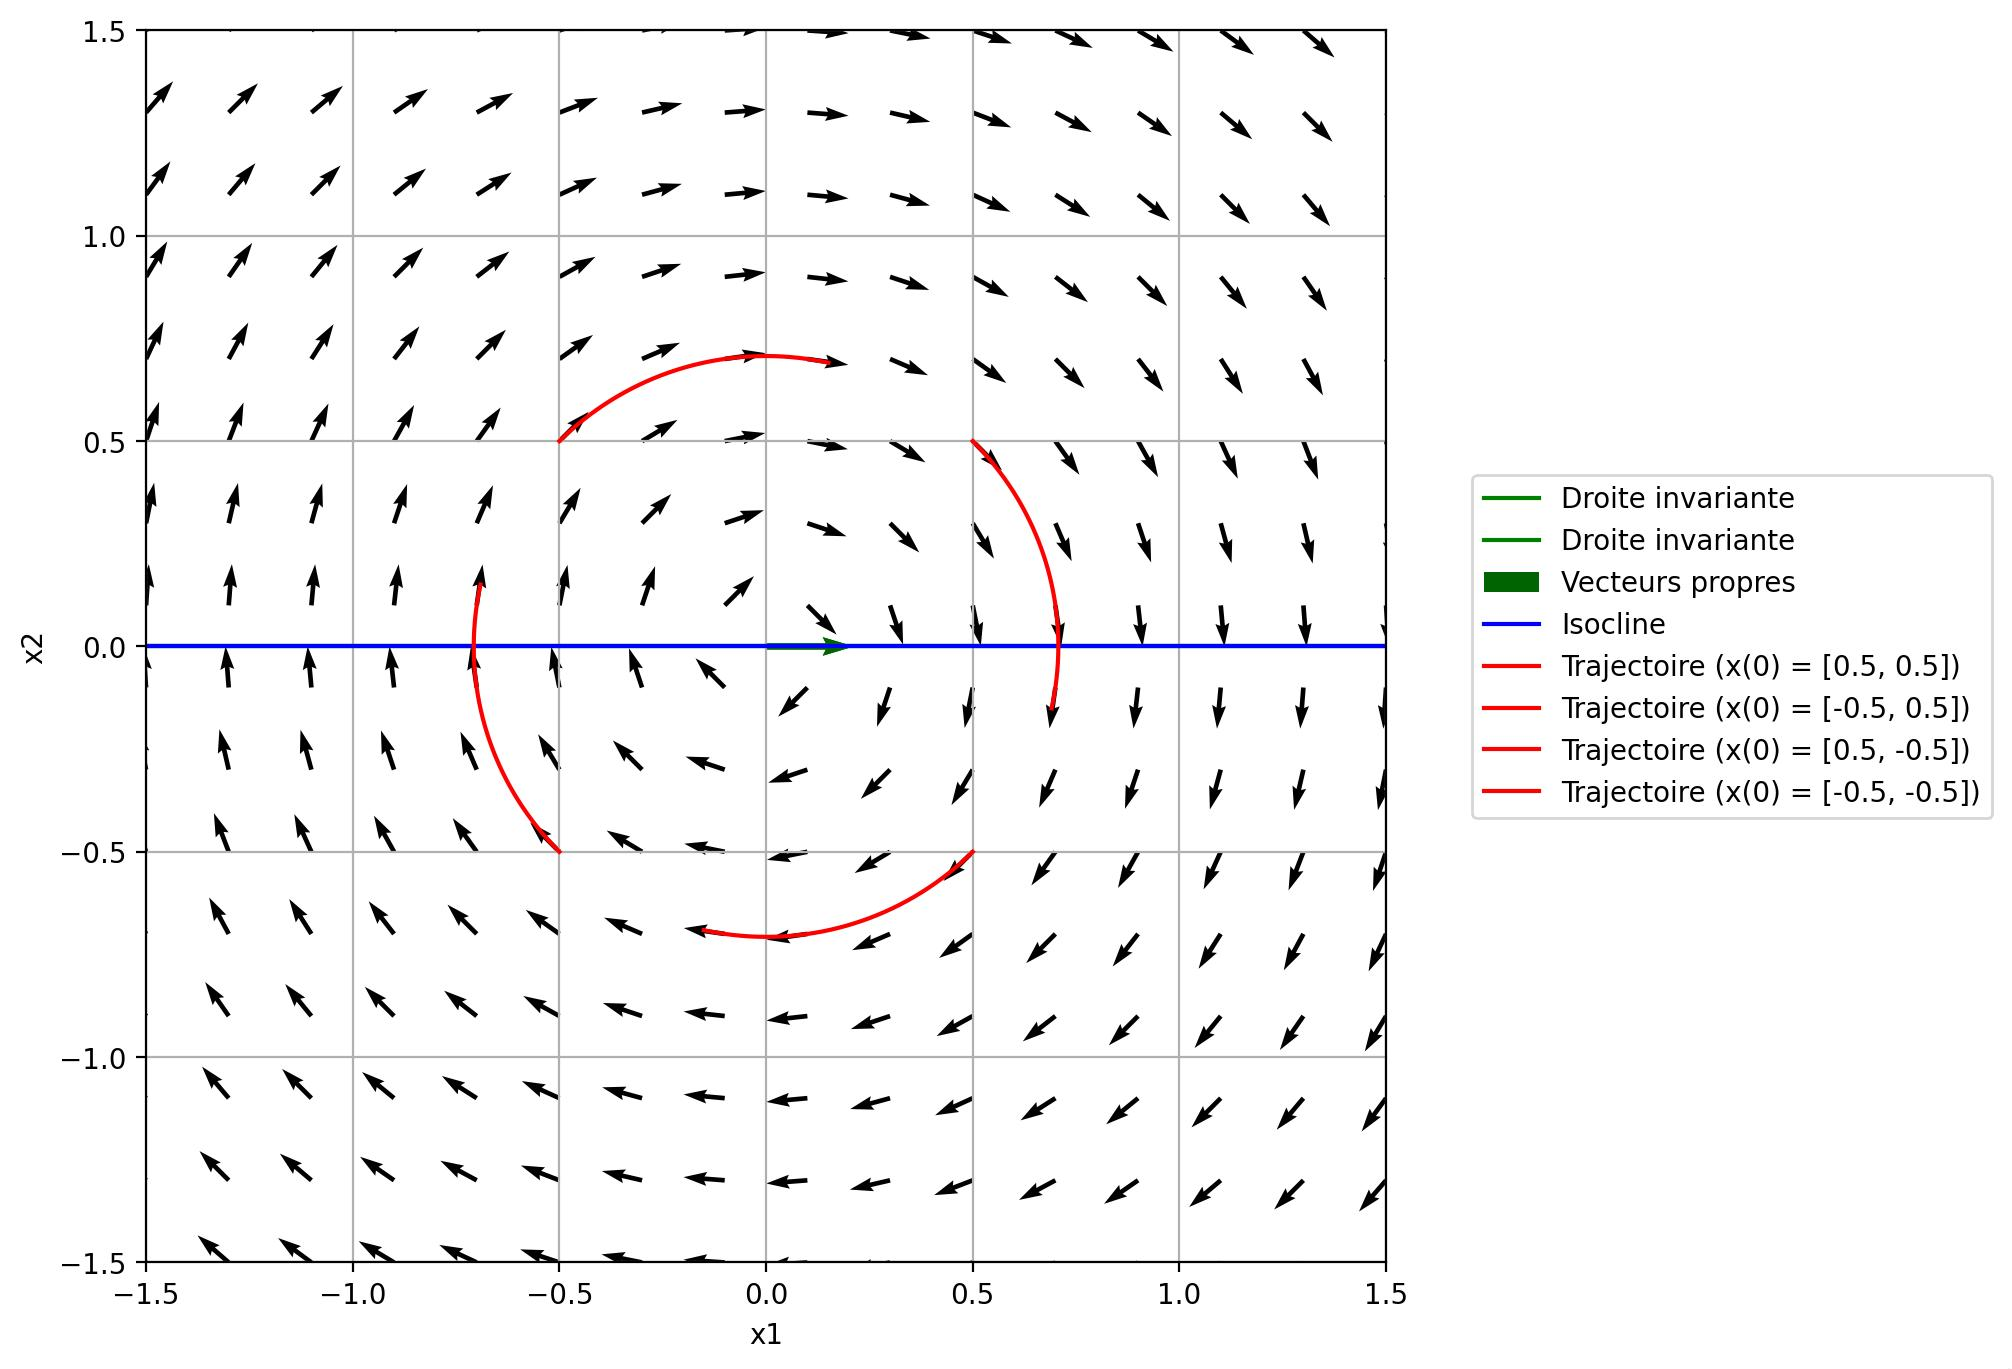
\includegraphics[width=\textwidth]{images/centre.jpg}
                    \caption{Exemple de centre}
                    \label{fig:centre}
                \end{figure}
                
                \item \textbf{Si $a < 0$ :} Le système est asymptotiquement stable, et les trajectoires convergent vers l'origine en spirale. L'origine est un \textit{foyer stable}. Un exemple est donné en figure \ref{fig:foyer_stable}, avec la matrice
                \begin{equation}
                    A = \begin{bmatrix} 0 & 1 \\ -1 & 1 \end{bmatrix}
                \end{equation}
                \begin{figure}[ht!]
                    \centering
                    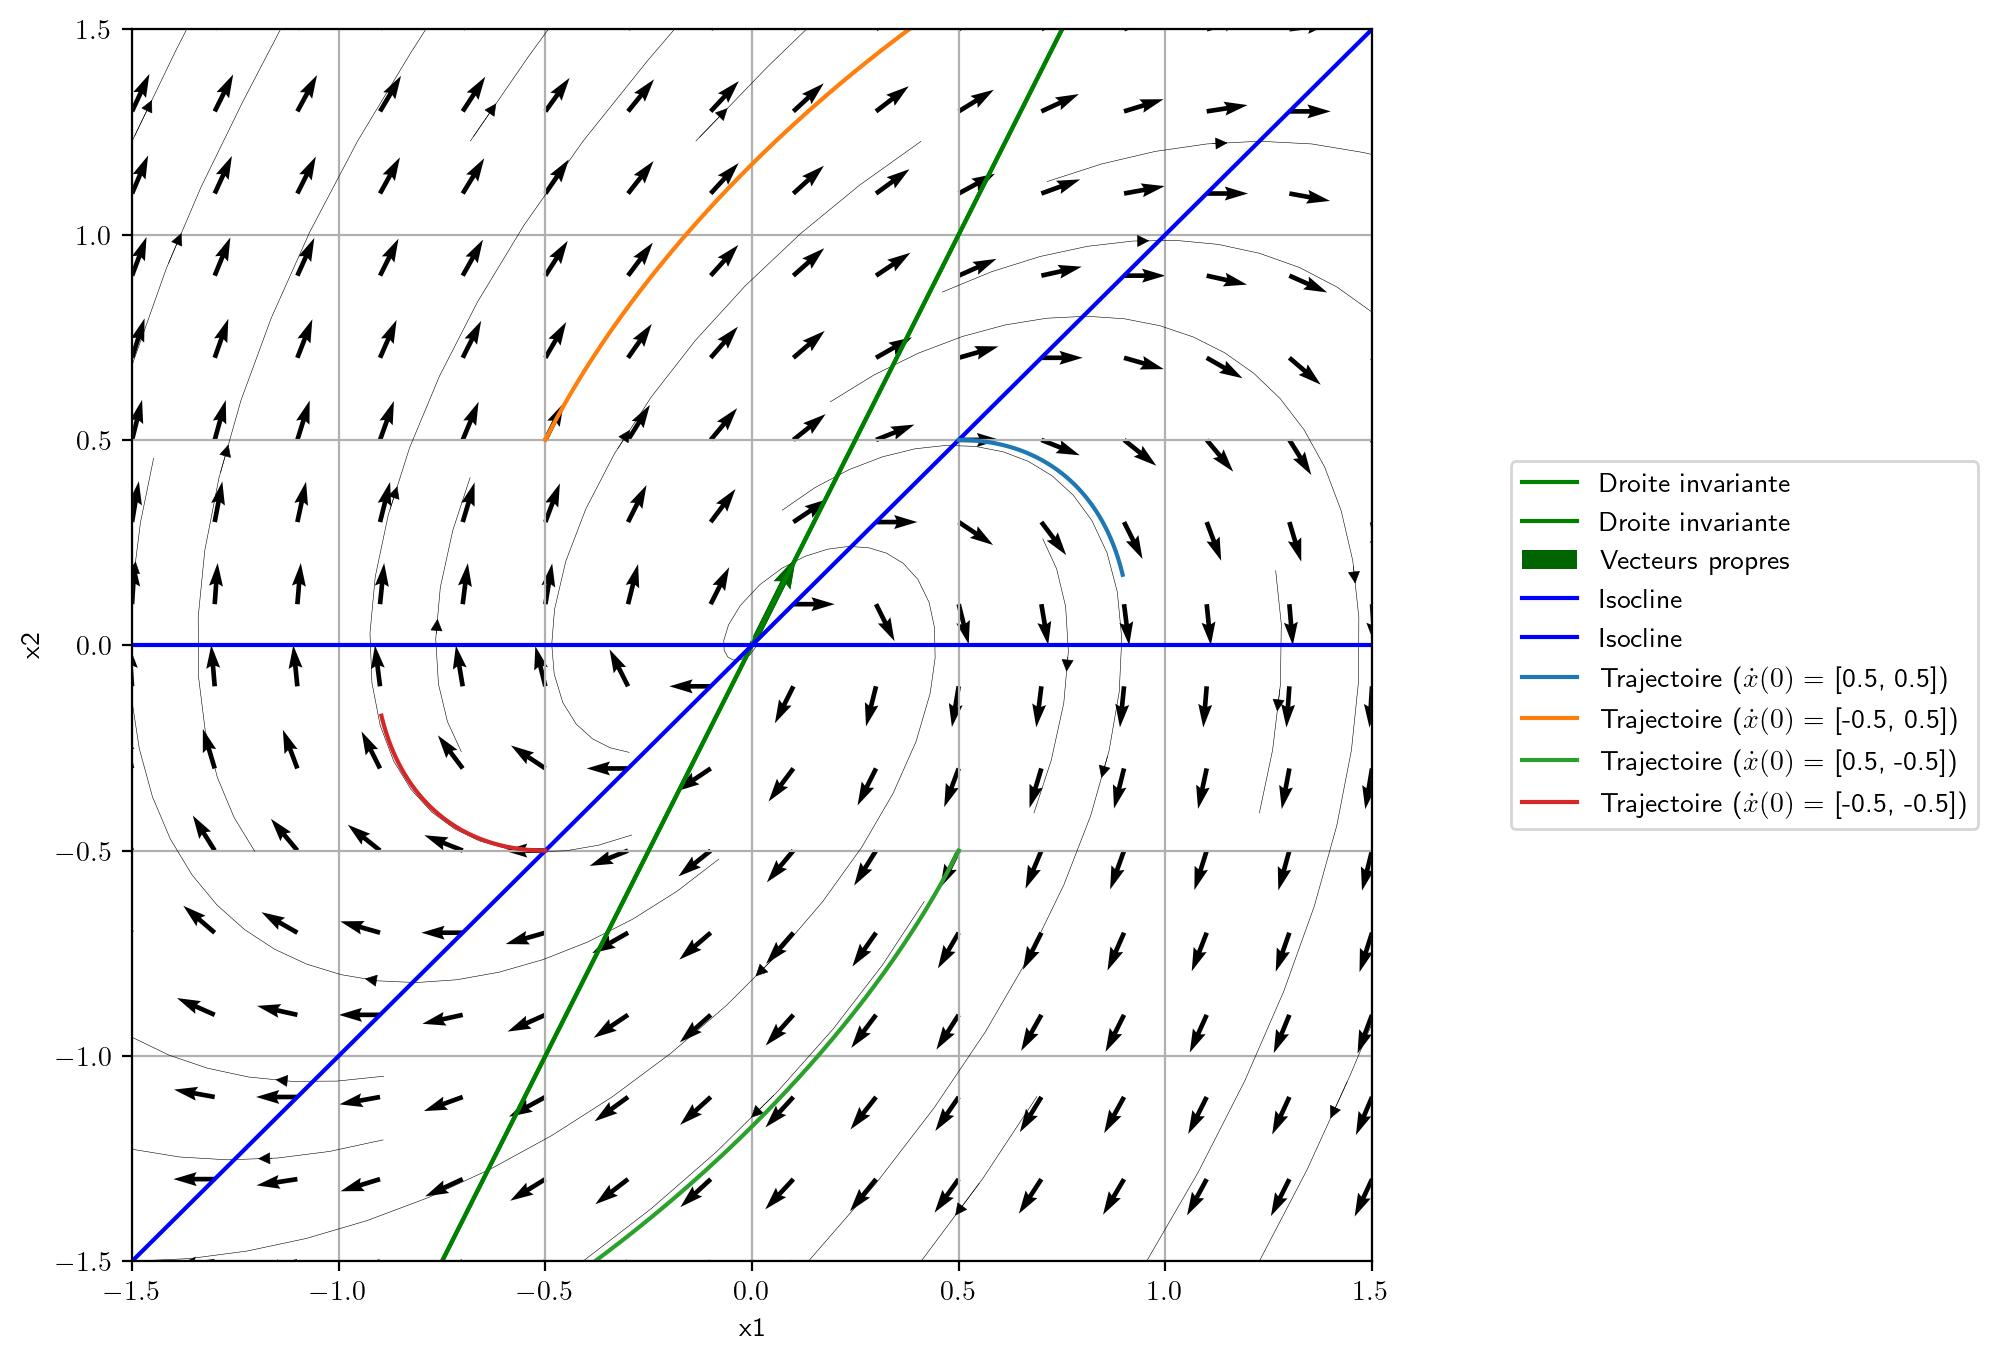
\includegraphics[width=\textwidth]{images/foyer_stable.jpg}
                    \caption{Exemple de foyer stable}
                    \label{fig:foyer_stable}
                \end{figure}
                
                \item \textbf{Si $a > 0$ :} Le système est instable, et les trajectoires divergent de l'origine en spirale. L'origine est un \textit{foyer instable}. Un exemple est donné en figure \ref{fig:foyer_instable}, avec la matrice
                \begin{equation}
                    A = \begin{bmatrix} 0 & 1 \\ -1 & -1 \end{bmatrix}
                \end{equation}
                \begin{figure}[ht!]
                    \centering
                    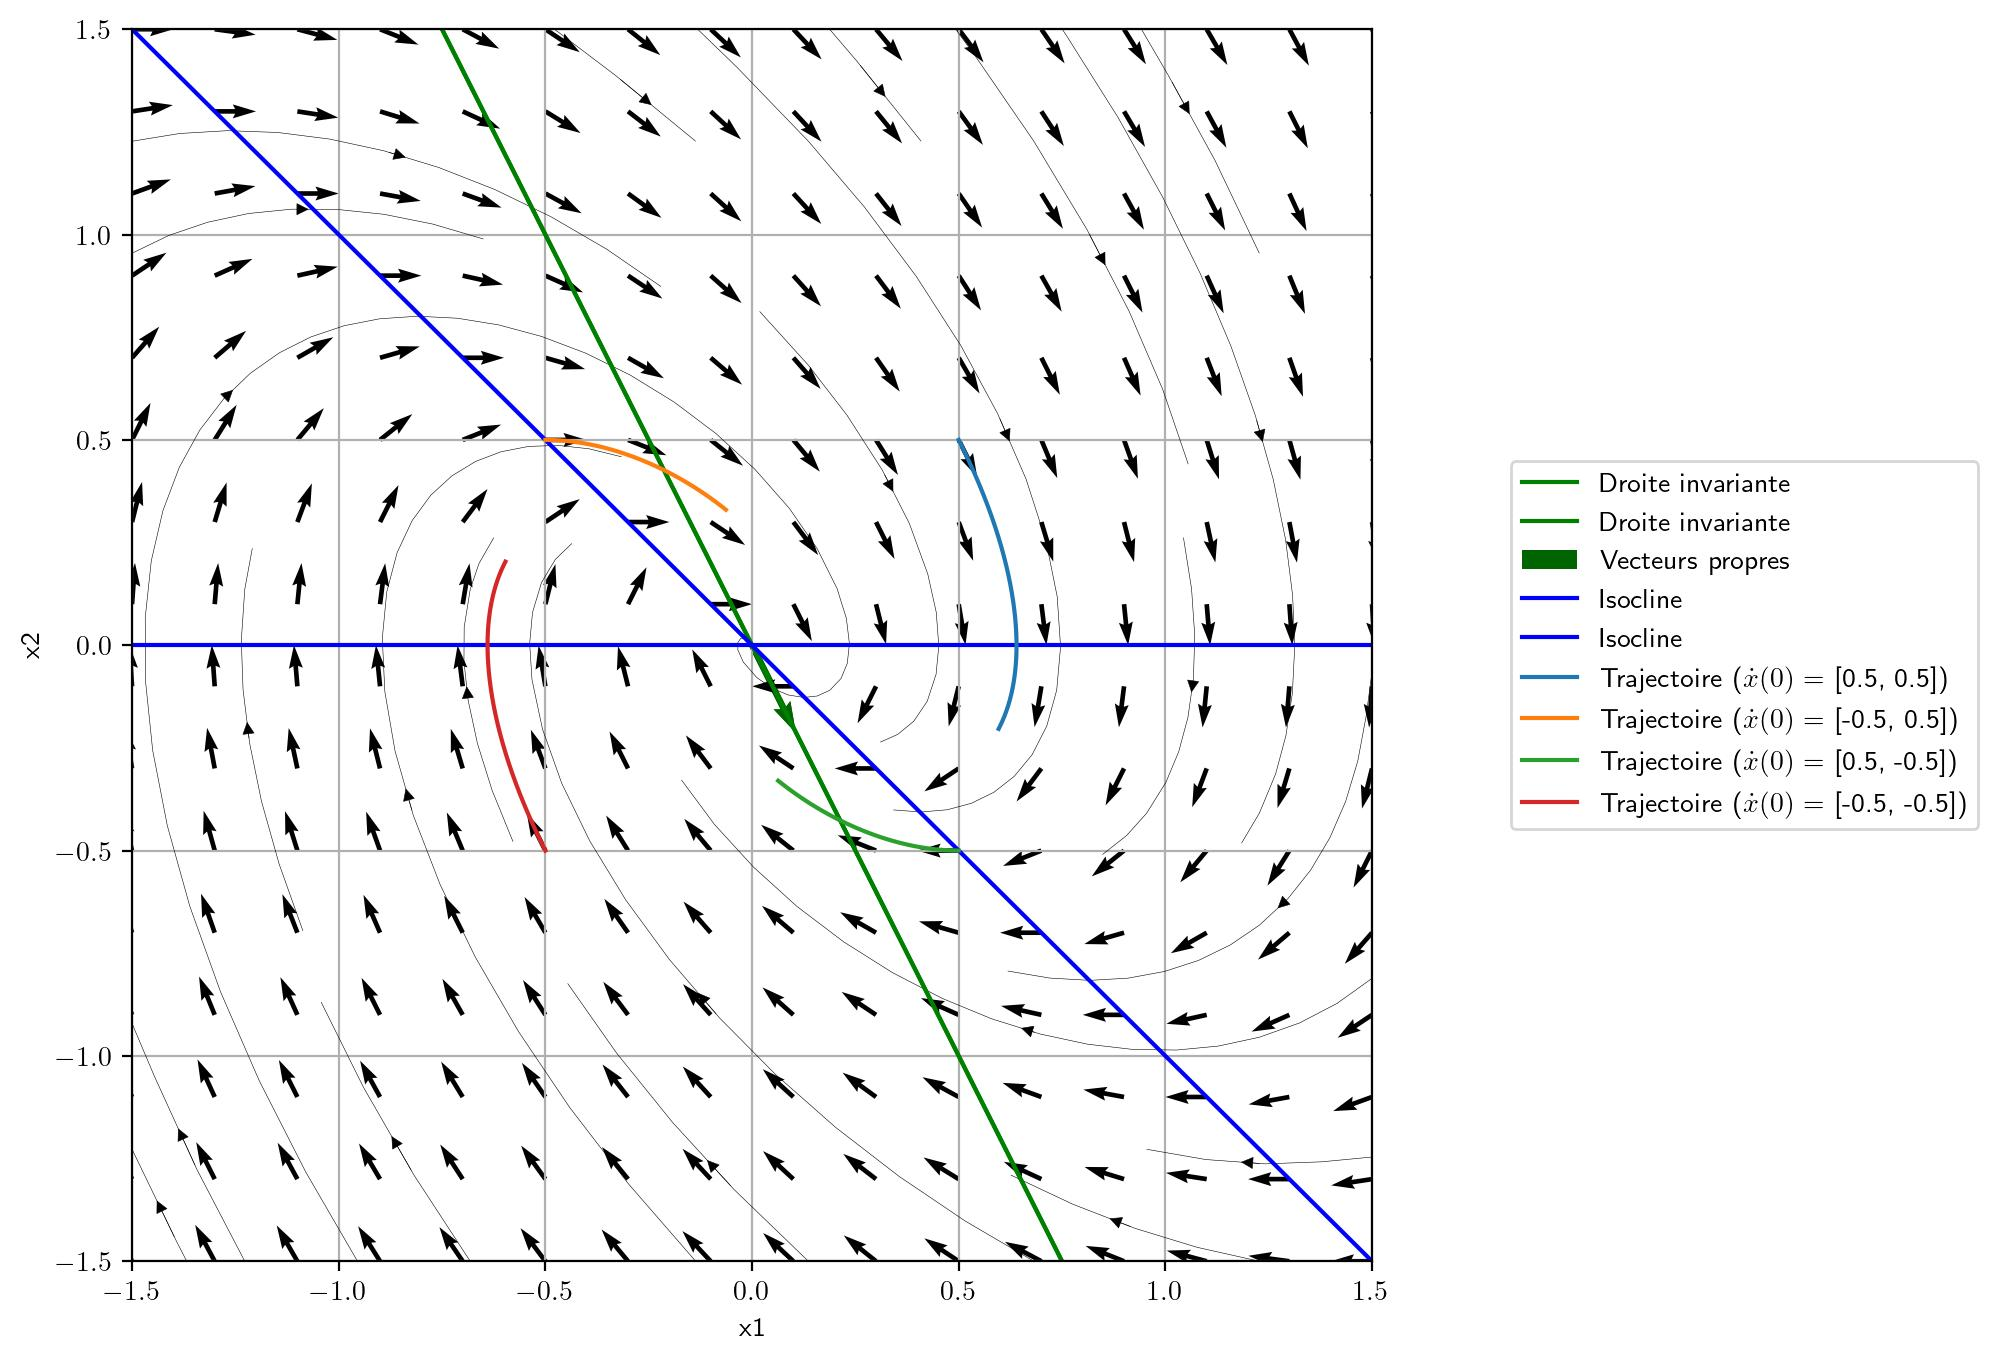
\includegraphics[width=\textwidth]{images/foyer_instable.jpg}
                    \caption{Exemple de foyer instable}
                    \label{fig:foyer_instable}
                \end{figure}
            \end{itemize}
            
            La direction de rotation (horaire ou anti-horaire) des trajectoires autour de l'origine dépend du signe de la partie imaginaire $b$ des valeurs propres.
            
    \section{Diagramme de Poincaré}\label{sec:poincare}
        L'étude de la stabilité des systèmes dynamiques linéaires a bénéficié des contributions pionnières de Henri Poincaré, mathématicien du XIX\textsuperscript{e} siècle, dont les travaux ont permis d'approfondir la compréhension des systèmes dynamiques et du comportement de leurs points d'équilibre. Le diagramme de Poincaré, qui relie la trace et le déterminant d'une matrice à la nature des points d'équilibre, est aujourd'hui un outil fondamental pour la classification de la stabilité des systèmes dynamiques linéaires. Cette approche permet de prédire rapidement la stabilité d'un système, en offrant une visualisation claire des régions de stabilité et d'instabilité sur le plan des valeurs propres.
        
        \subsection{Trace et déterminant de la matrice $A$}
            La classification des points d'équilibre d'un système linéaire peut ainsi être résumée de manière compacte en utilisant la trace et le déterminant de la matrice $A$. En effet, les valeurs propres de $A$, notées $\lambda_1$ et $\lambda_2$, sont notamment calculables par l'expression
            \begin{equation}
                \lambda_{1,2} = \frac{\Tr(A) \pm \sqrt{\Tr(A)^2 - 4 \det(A)}}{2}
            \end{equation}
            obtenue en développant l'équation caractéristique (voir équation \ref{eq:equation_caracteristique}).
            
            Cette formule utilise deux éléments que nous savons calculer facilement depuis l'équation \ref{eq:valeurs_propres}: la trace $\Tr(A)$ et le déterminant $\det(A)$ de la matrice $A$. Ceux-ci permettent de déterminer la nature des valeurs propres, qu'elles soient réelles ou complexes, positives ou négatives, montrant ainsi la stabilité des points d'équilibre associés. En particulier, le discriminant 
            \begin{equation}
                \Tr(A)^2 - 4 \det(A) = 0
            \end{equation}
            définit une parabole sur le plan $(\Tr(A), \det(A))$ qui sépare différentes régions de stabilité dans le système dynamique. Cette parabole représente la transition entre les valeurs propres réelles et complexes, et sa position est cruciale pour interpréter les comportements qualitatifs des trajectoires. 

            Le diagramme de Poincaré, montré dans la figure \ref{fig:poincare}, présente cette classification en fonction de la trace et du déterminant de $A$, indiquant les différentes régions de stabilité et le type de points d'équilibre que l'on peut rencontrer.
            \begin{figure}[ht!]
                \centering
                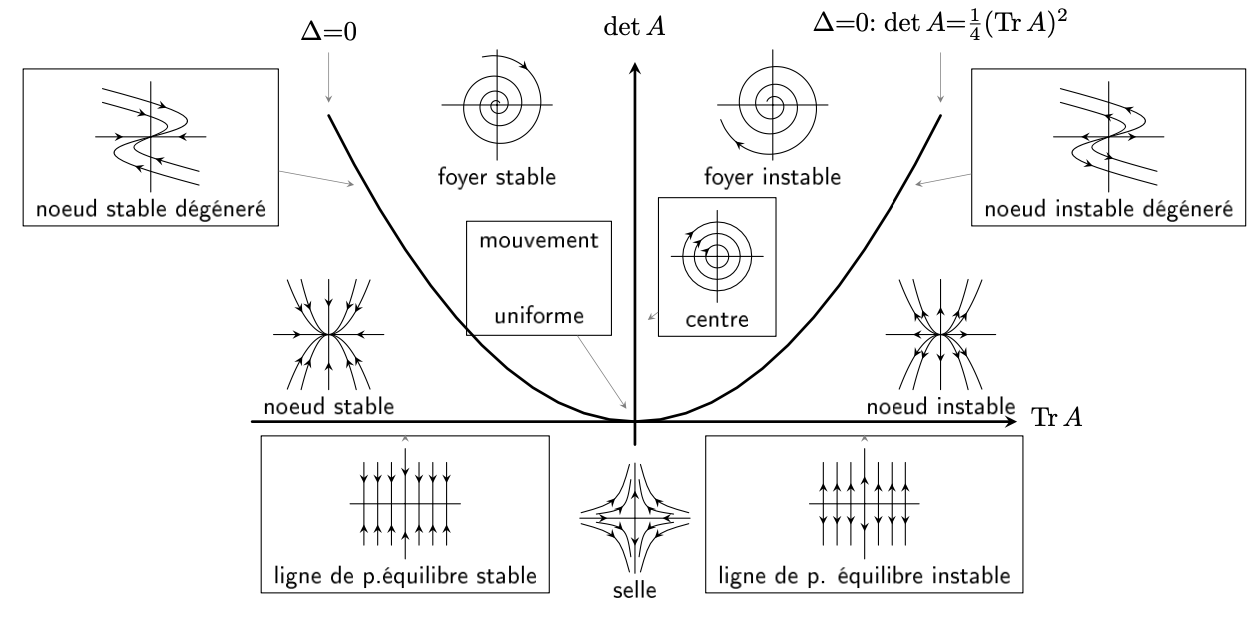
\includegraphics[width=\textwidth]{images/poincare.png}
                \caption{Graphique de classification des points d'équilibre selon la trace et le déterminant de la matrice décrivant le système}
                \label{fig:poincare}
            \end{figure}

            On visualise sur cette figure plusieurs régularités:
            \begin{itemize}
                \item Si la trace de la matrice est négative, le système est stable, si elle est strictement positive, elle est instable. Si la trace est nulle, le système décrit soit un centre, soit un mouvement uniforme.
                \item Si le point $\begin{bmatrix}\Tr(A)\\\det A\end{bmatrix}$ se trouve au-dessus de la parabole d'équation $\Tr(A)^2 - 4 \det(A) = 0$, le système est rotatif autour de son point d'équilibre.
                \item De manière plus intuitive, les mouvements intermédiaires (sur l'axe $\det A = 0$,  sur la parabole, ou sur l'axe $\Tr(A) = 0$) peuvent être vus comme des comportements limites entre ceux des régions qui les entourent. Par exemple, un centre ressemble à un foyer, qui n'est ni stable ni instable.
            \end{itemize}
            
    \section{Exercices}
        Nous suivons la même forme d'exercices que vue précédemment.
        Vous devez:
        \begin{enumerate}
            \item définir la matrice des coefficients~;
            \item définir l'équation caractéristique~;
            \item calculer les valeurs propres~;
            \item déterminer les vecteurs propres, et les trajectoires associées~;
            \item dessiner les vecteurs vitesses pour des points bien choisis~;
            \item dessiner la trajectoire du système pour ces conditions initiales pour un intervalle de temps donné~;
            \item Vérifier que la région sur le diagramme de Poincaré correspond effectivement au comportement observé.
        \end{enumerate}
        
        \subsection{Exercice 1: système non-simple}
            \begin{exercise}{Système non-simple}
                Effectuez les étapes présentées à la section précédente pour le système
                \begin{equation}
                    \begin{cases}
                        \dot{x}_1(t) = x_2(t)\\
                        \dot{x}_2(t) = x_2(t)
                    \end{cases}
                \end{equation}
            \end{exercise}
            Tracez les vecteurs vitesses en $x = \begin{bmatrix}0 \\ 1\end{bmatrix}$, $\begin{bmatrix}0 \\ -1\end{bmatrix}$, $\begin{bmatrix}-1 \\ 0\end{bmatrix}$ et $\begin{bmatrix}0 \\ -1\end{bmatrix}$. Tracez les trajectoires démarrant en $x = \begin{bmatrix}0 \\ 1\end{bmatrix}$ et en $x = \begin{bmatrix}-0.5 \\ -1\end{bmatrix}$.
            La solution numérique est donnée en figure \ref{fig:pdp_exercice_2_1}.
            \begin{figure}[ht!]
                \centering
                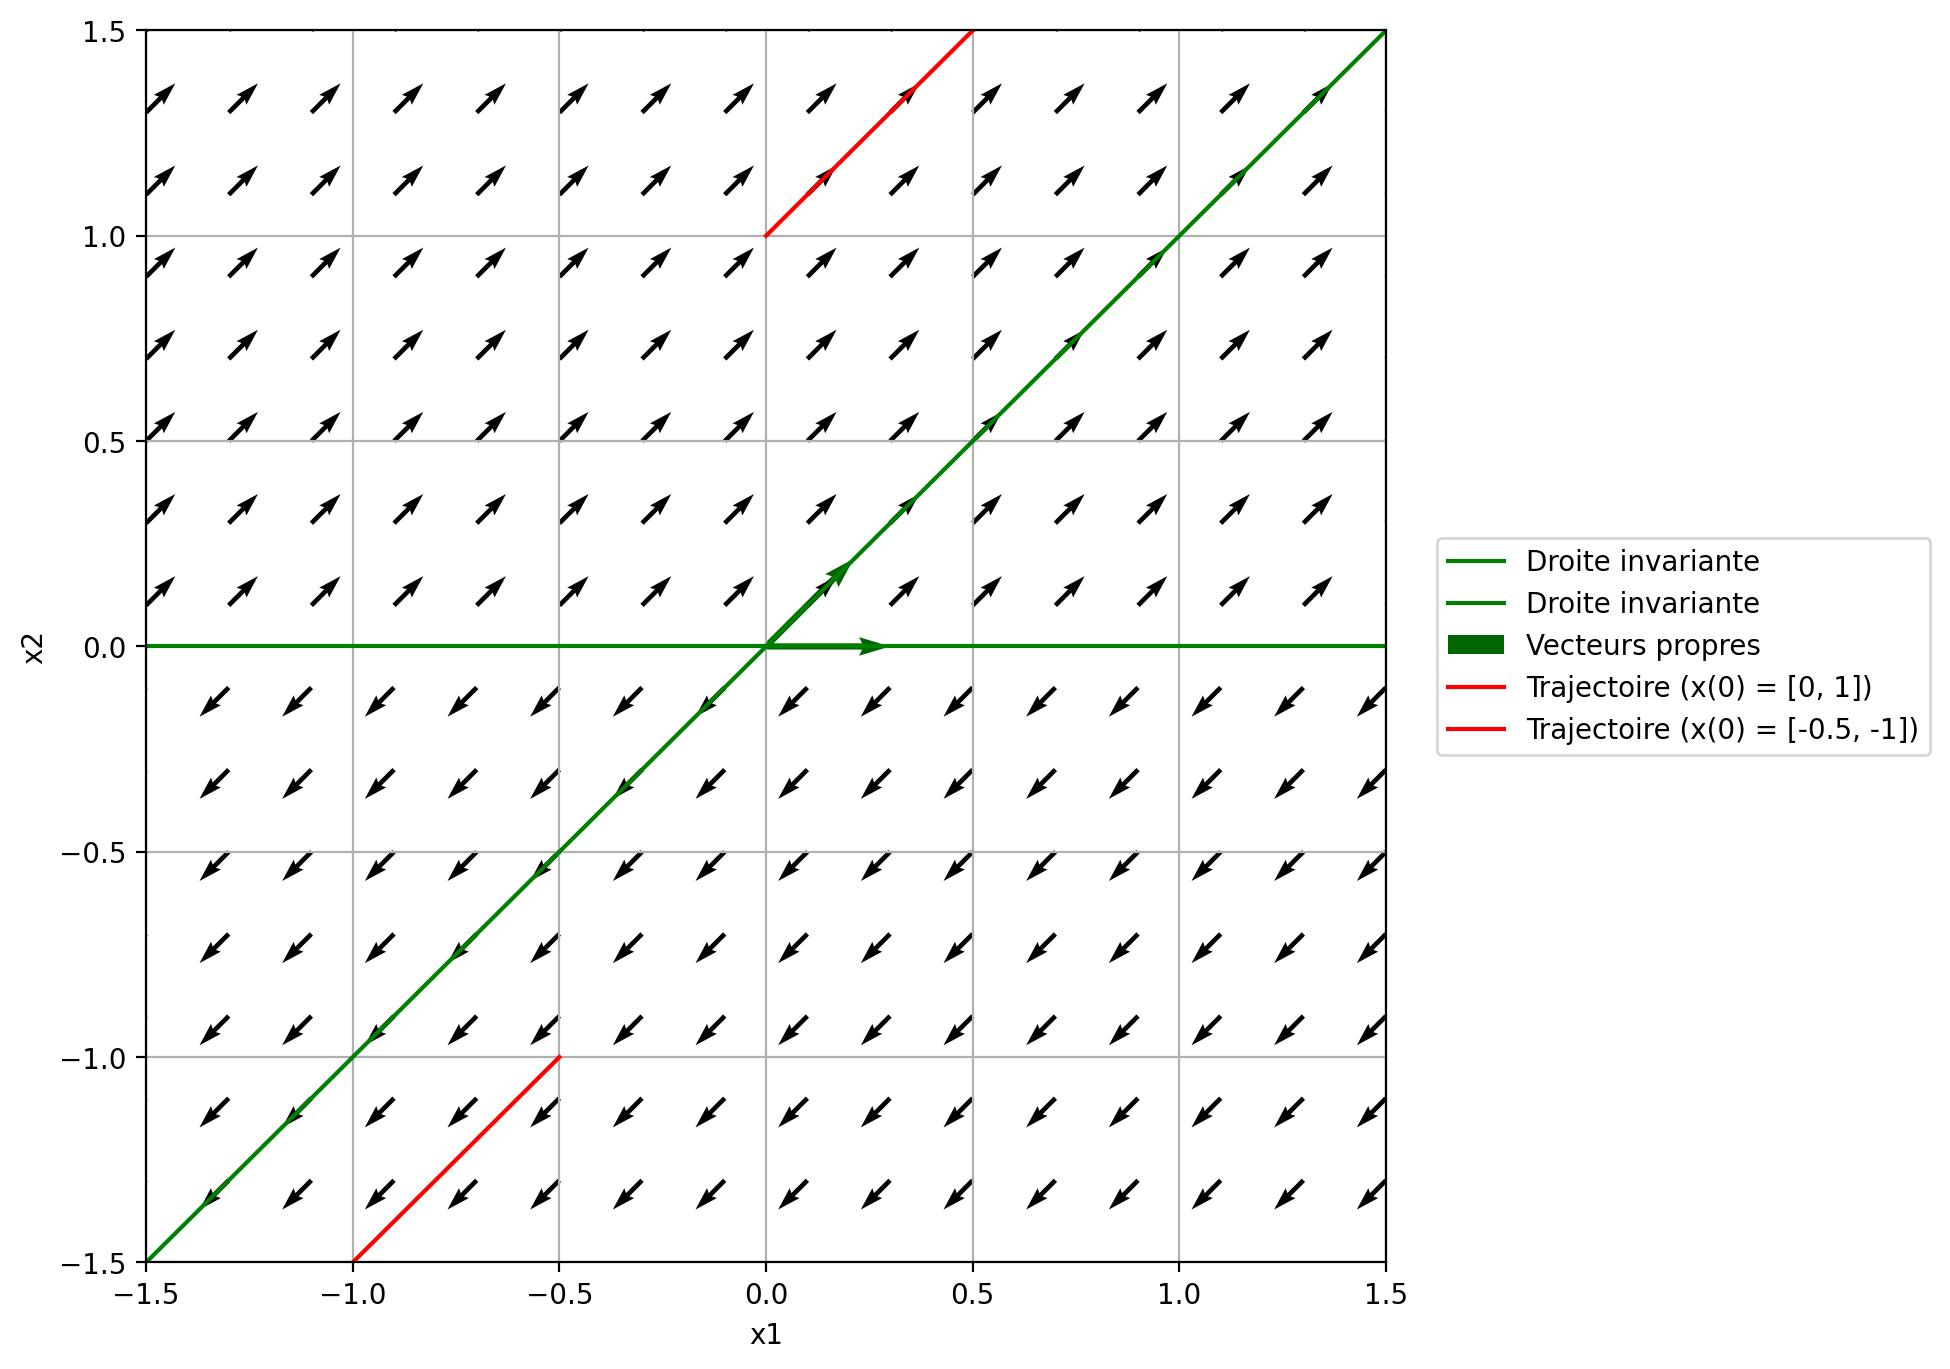
\includegraphics[width=\textwidth]{images/pdp_exercice_2_1.jpg}
                \caption{Solution numérique de l'exercice 1}
                \label{fig:pdp_exercice_2_1}
            \end{figure}

        \subsection{Exercice 2: centre}
            \begin{exercise}{Centre}
                Prenez le système
                \begin{equation}
                    \begin{cases}
                        \dot{x}_1(t) = -x_2(t)\\
                        \dot{x}_2(t) = x_1(t)
                    \end{cases}
                \end{equation}
            \end{exercise}
            Tracez les vecteurs vitesses en $x = \begin{bmatrix}0 \\ 1\end{bmatrix}$, $\begin{bmatrix}0 \\ -1\end{bmatrix}$, $\begin{bmatrix}-1 \\ 0\end{bmatrix}$ et $\begin{bmatrix}0 \\ -1\end{bmatrix}$. Tracez les trajectoires démarrant en $x = \begin{bmatrix}0 \\ 1\end{bmatrix}$ et en $x = \begin{bmatrix}-0.5 \\ -1\end{bmatrix}$.
            La solution numérique est donnée en figure \ref{fig:pdp_exercice_2_2}.
            \begin{figure}[ht!]
                \centering
                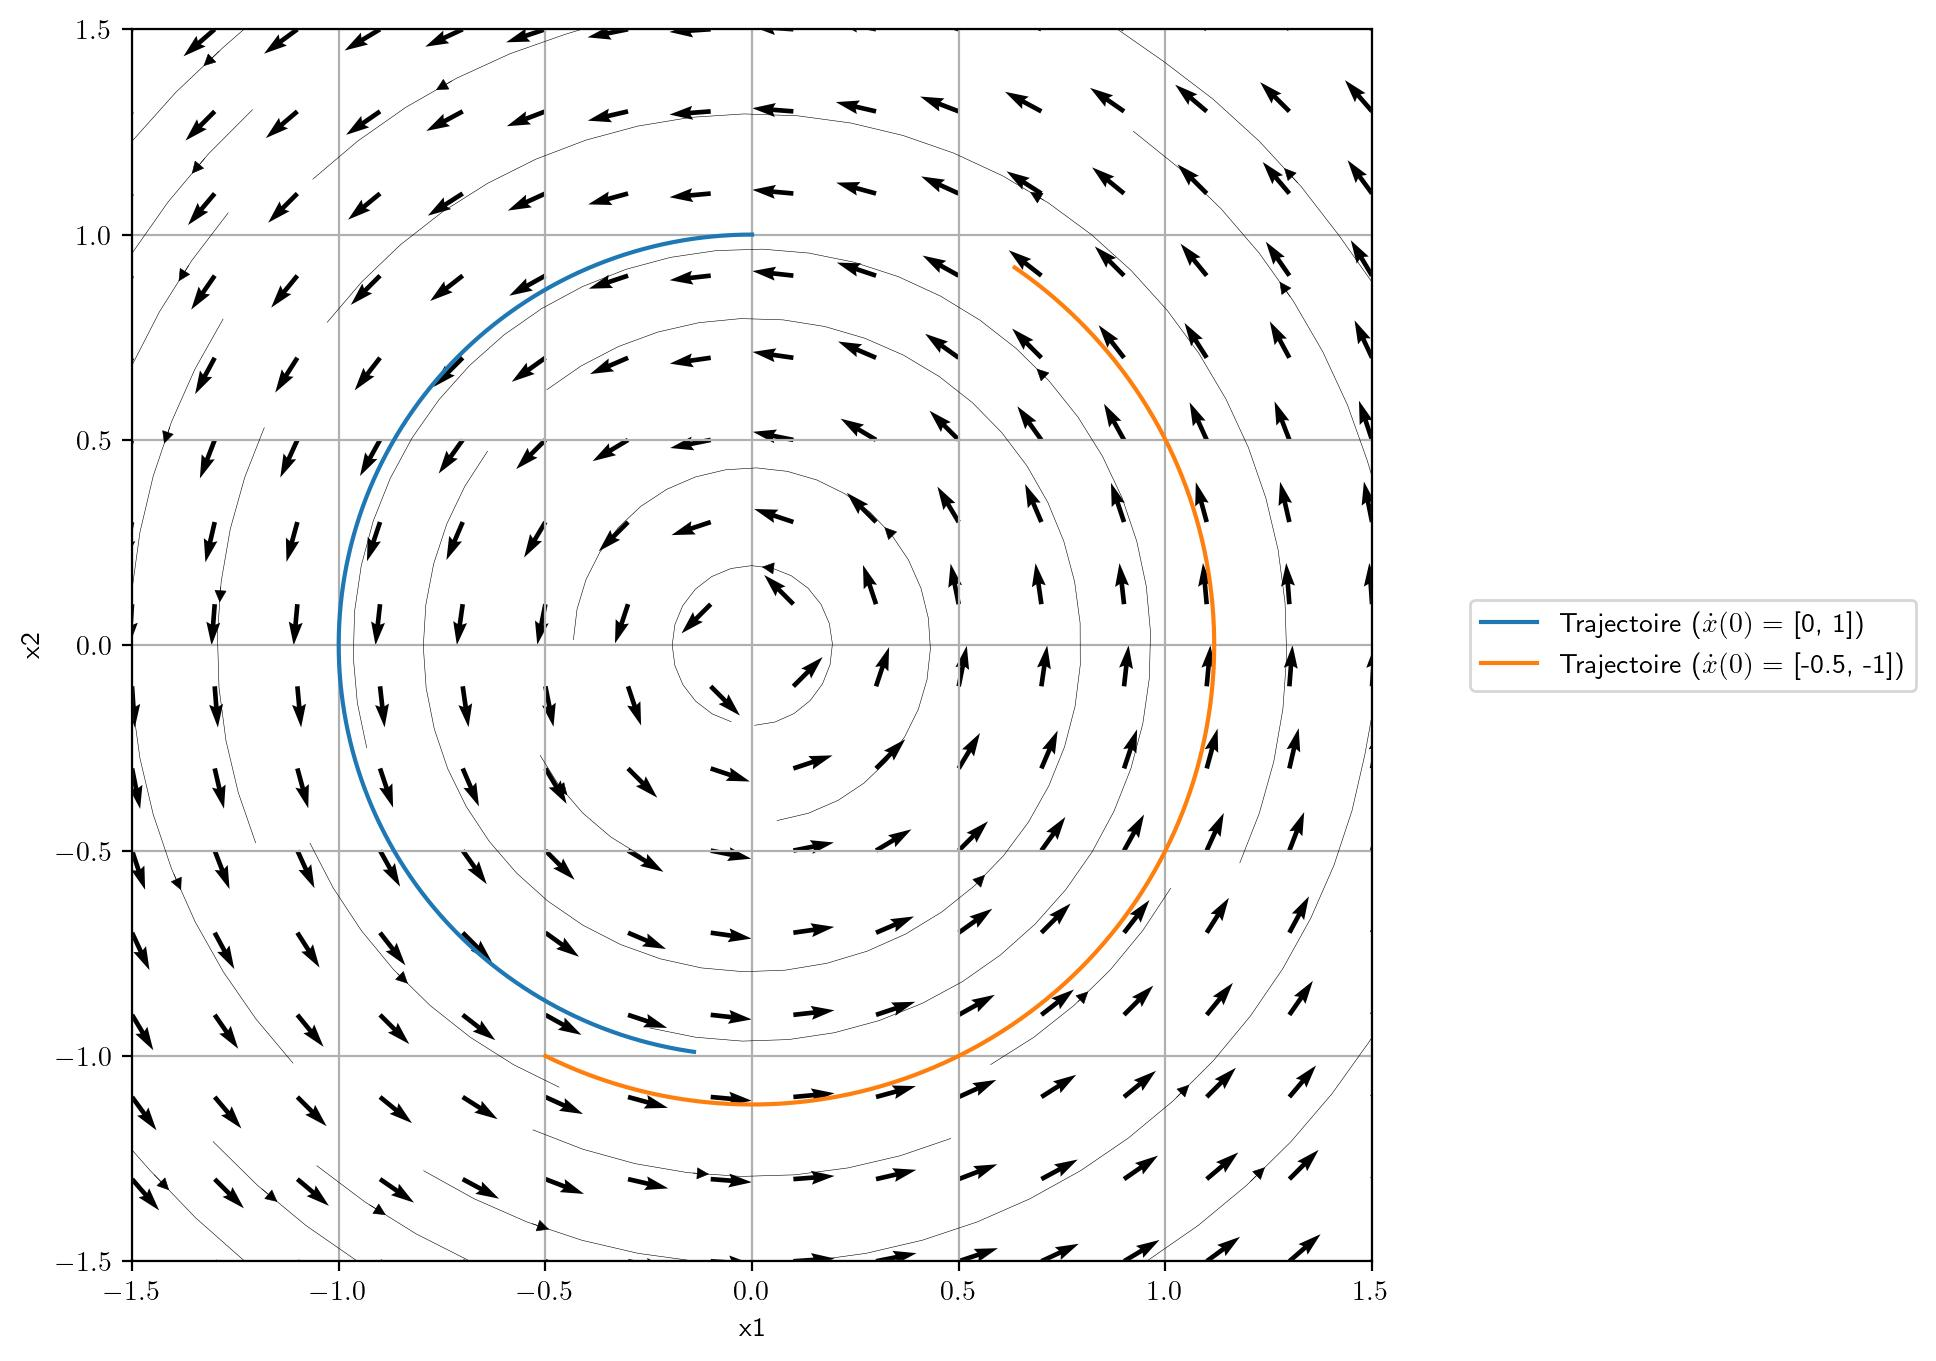
\includegraphics[width=\textwidth]{images/pdp_exercice_2_2.jpg}
                \caption{Solution numérique de l'exercice 2}
                \label{fig:pdp_exercice_2_2}
            \end{figure}

        \subsection{Exercice 3: foyer stable}
            \begin{exercise}{Foyer stable}
                Finalement, pour le système
                \begin{equation}
                    \begin{cases}
                        \dot{x}_1(t) = \frac{x_1(t)}{3} - 2 x_2(t)\\
                        \dot{x}_2(t) = 3 x_1(t) - x_2(t)
                    \end{cases}
                \end{equation}
            \end{exercise}
            Tracez les vecteurs vitesses en $x = \begin{bmatrix}0 \\ 1\end{bmatrix}$, $\begin{bmatrix}0 \\ -1\end{bmatrix}$, $\begin{bmatrix}-1 \\ 0\end{bmatrix}$ et $\begin{bmatrix}0 \\ -1\end{bmatrix}$. Tracez les trajectoires démarrant en $x = \begin{bmatrix}0 \\ 1\end{bmatrix}$ et en $x = \begin{bmatrix}-0.5 \\ -1\end{bmatrix}$.
            La solution numérique est donnée en figure \ref{fig:pdp_exercice_2_3}.
            \begin{figure}[ht!]
                \centering
                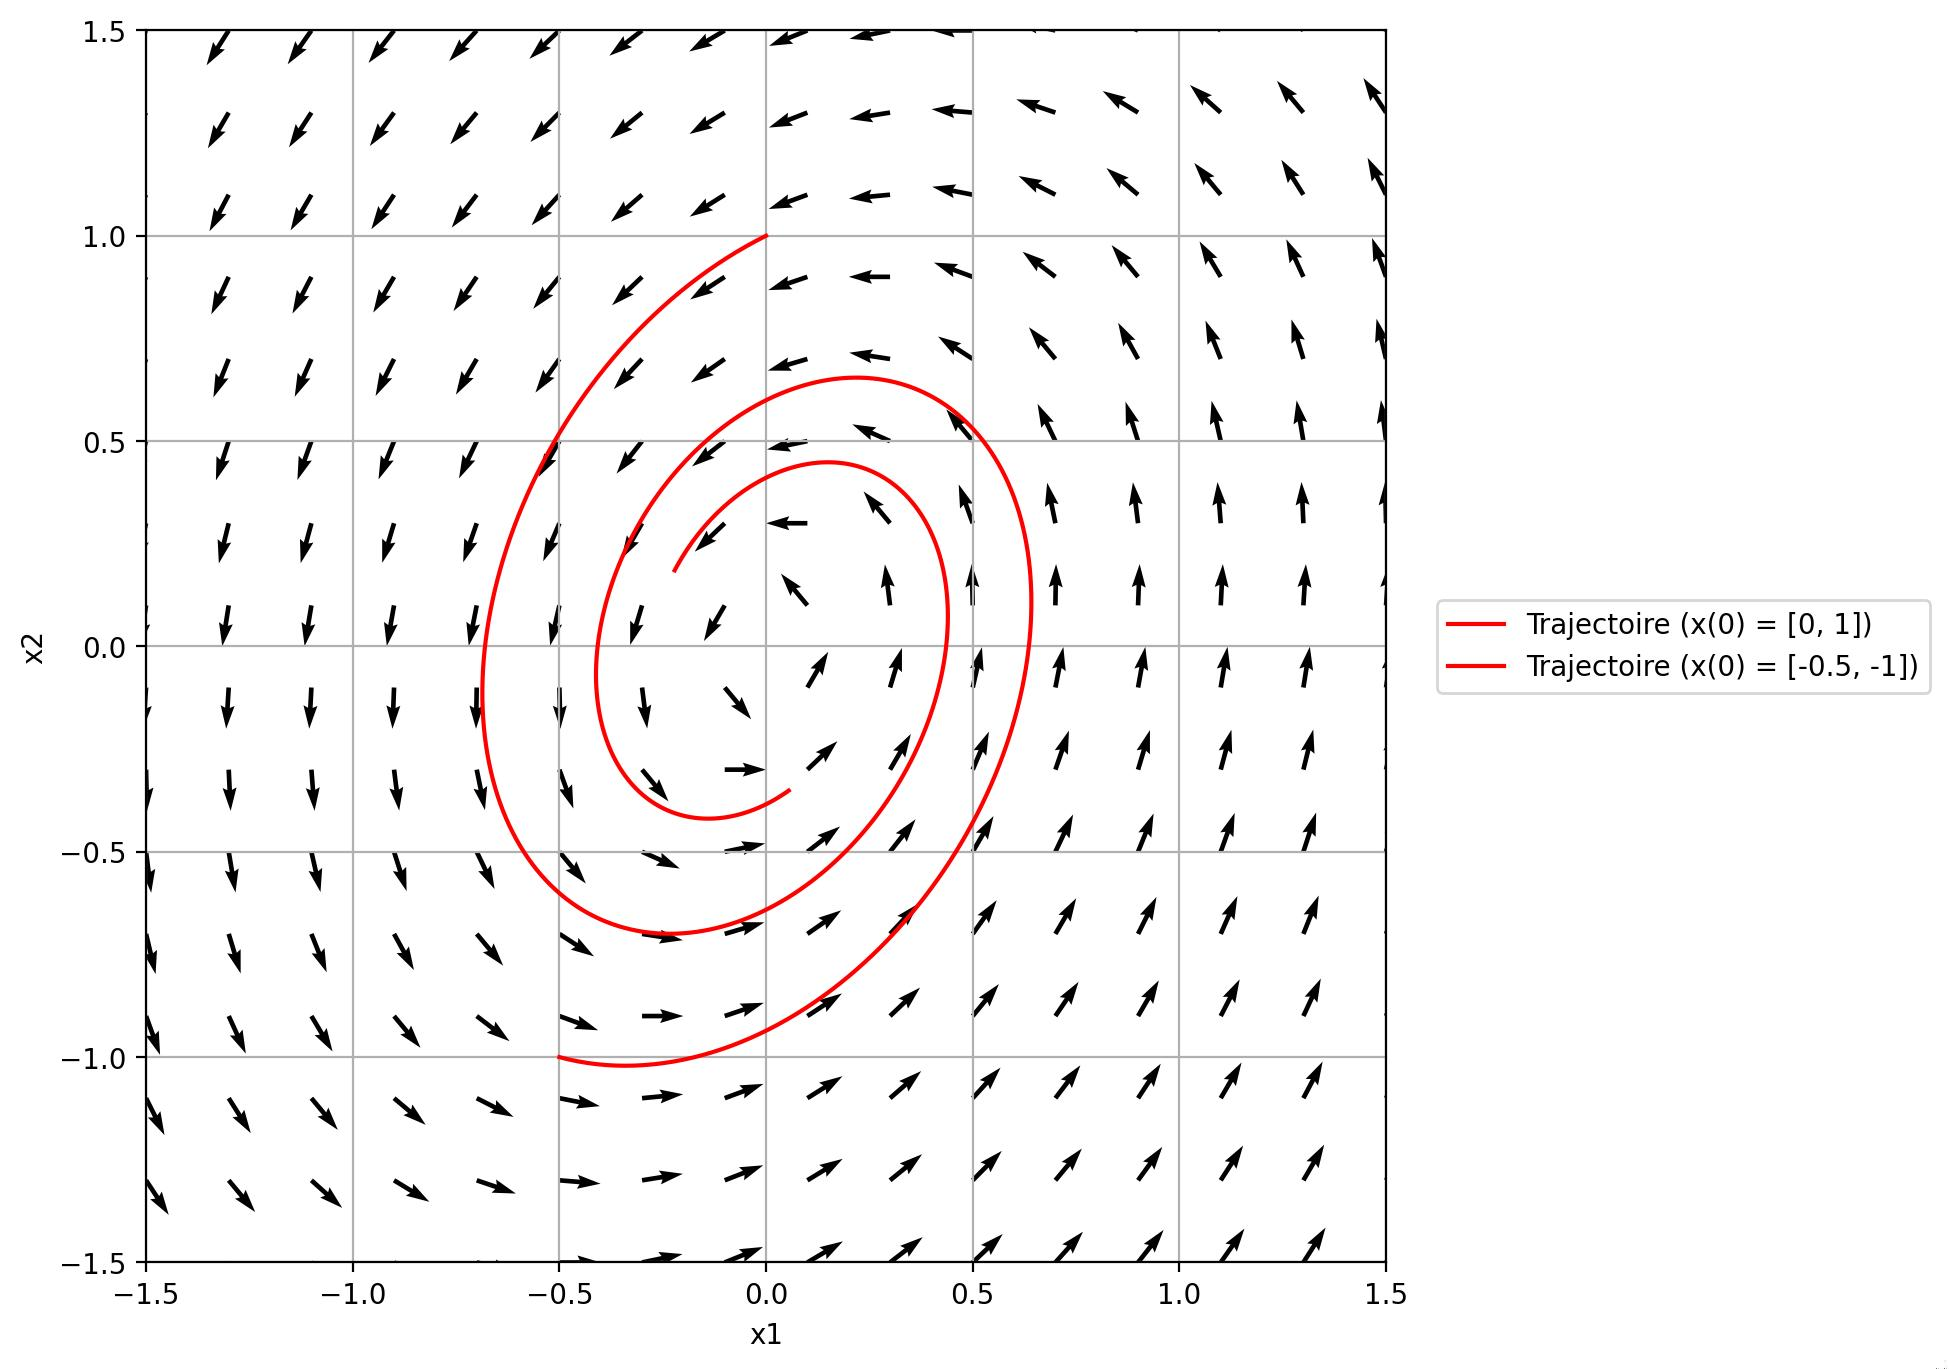
\includegraphics[width=\textwidth]{images/pdp_exercice_2_3.jpg}
                \caption{Solution numérique de l'exercice 3}
                \label{fig:pdp_exercice_2_3}
            \end{figure}
    
    \section{Comportement des trajectoires pour un temps tendant vers l'infini}
        Rappelons-nous que pour un système
        \begin{equation}
            \dot{x}(t) = A x(t)
        \end{equation}
        où $A$ est une matrice $2 \times 2$, la solution générale de ce système est de la forme: \robin{si les valeurs propres sont distinctes}
        \begin{equation}
            x(t) = c_1 e^{\lambda_1 t} \overrightarrow{v_1} + c_2 e^{\lambda_2 t} \overrightarrow{v_2}
        \end{equation}
        c'est-à-dire
        \begin{equation}
            \begin{cases}
                x_1(t) = c_1 e^{\lambda_1 t} v_{11} + c_2 e^{\lambda_2 t} v_{21} \\
                x_2(t) = c_1 e^{\lambda_1 t} v_{12} + c_2 e^{\lambda_2 t} v_{22}
            \end{cases}
        \end{equation}
        où $\lambda_1$ et $\lambda_2$ sont les valeurs propres de $A$, et $\overrightarrow{v_1}$ et $\overrightarrow{v_2}$ les vecteurs propres associés. Cette solution montre que le comportement du système est une superposition de deux composantes exponentielles : une dans la direction de $\overrightarrow{v_1}$ et l'autre dans la direction de $\overrightarrow{v_2}$. La stabilité et l’alignement final des trajectoires dépendent de la nature des valeurs propres.

        \subsection{Cas des valeurs propres réelles et négatives}
            Lorsque les deux valeurs propres sont réelles et négatives, toutes les trajectoires convergent vers l'origine pour un intervalle de temps tendant vers l'infini. Un tel système est dit asymptotiquement stable. Plus précisément, si $\lambda_1 < \lambda_2 < 0$, alors:
            \begin{equation}
                \lim_{t \to \infty} \frac{x_2(t)}{x_1(t)} = \frac{v_{22}}{v_{21}}
            \end{equation}
            Dans ce cas, la direction de la trajectoire s'aligne sur le vecteur propre $ \overrightarrow{v_2}$, associé à la plus petite valeur propre en valeur absolue, et donc à la décroissance la plus lente. Ce phénomène est dû la domination de la composante exponentielle de $\overrightarrow{v_2}$ dans le comportement à long terme du système.

        \subsection{Cas des valeurs propres réelles et positives}
            Si les deux valeurs propres sont réelles et positives, le système est instable: les deux composantes du mouvement divergent de manière exponentielle. Si $\lambda_1 > \lambda_2 > 0$, alors, dans le temps, la direction de la trajectoire s’aligne sur le vecteur propre $\overrightarrow{v_1}$, correspondant à la valeur propre la plus grande. Cette composante de divergence rapide domine alors l'évolution du système, entraînant une divergence rapide des trajectoires pour un intervalle de temps tendant vers l'infini.
            
            Déterminer ces informations est cruciale pour le dessin qualitatif des trajectoires des systèmes dynamiques, en permettant d'anticiper l'évolution des états du système à partir de la configuration initiale.
            
    \section{Les isoclines et leur rôle dans la dynamique}
        \begin{definition}{Isoclines}
            Les isoclines sont les courbes pour lesquelles l'une des dérivées du système est nulle.
        \end{definition}
        Elles sont essentielles pour comprendre la dynamique des trajectoires dans le portrait de phases :
        \begin{itemize}
            \item Les isoclines divisent le plan en régions où les signes de $\dot{x}_1$ et $\dot{x}_2$ changent, determinant la direction des vecteurs vitesse.
            \item Sur les isoclines, les vecteurs vitesse sont alignés horizontalement (lorsque $\dot{x}_2 = 0$) ou verticalement (lorsque $\dot{x}_1 = 0$), rajoutant une série de vecteurs vitesse faciles à tracer.
        \end{itemize}
        La figure \ref{fig:isoclines} montre les isoclines et les vecteurs vitesse associés au système décrit par la matrice
        \begin{equation}
            A = \begin{bmatrix} 1 & 2 \\ -1 & 1 \end{bmatrix}
        \end{equation}
        où l'on voit bien que les vecteurs vitesse des points appartenant aux isoclines sont horizontaux ou verticaux.
        \begin{figure}[ht!]
            \centering
            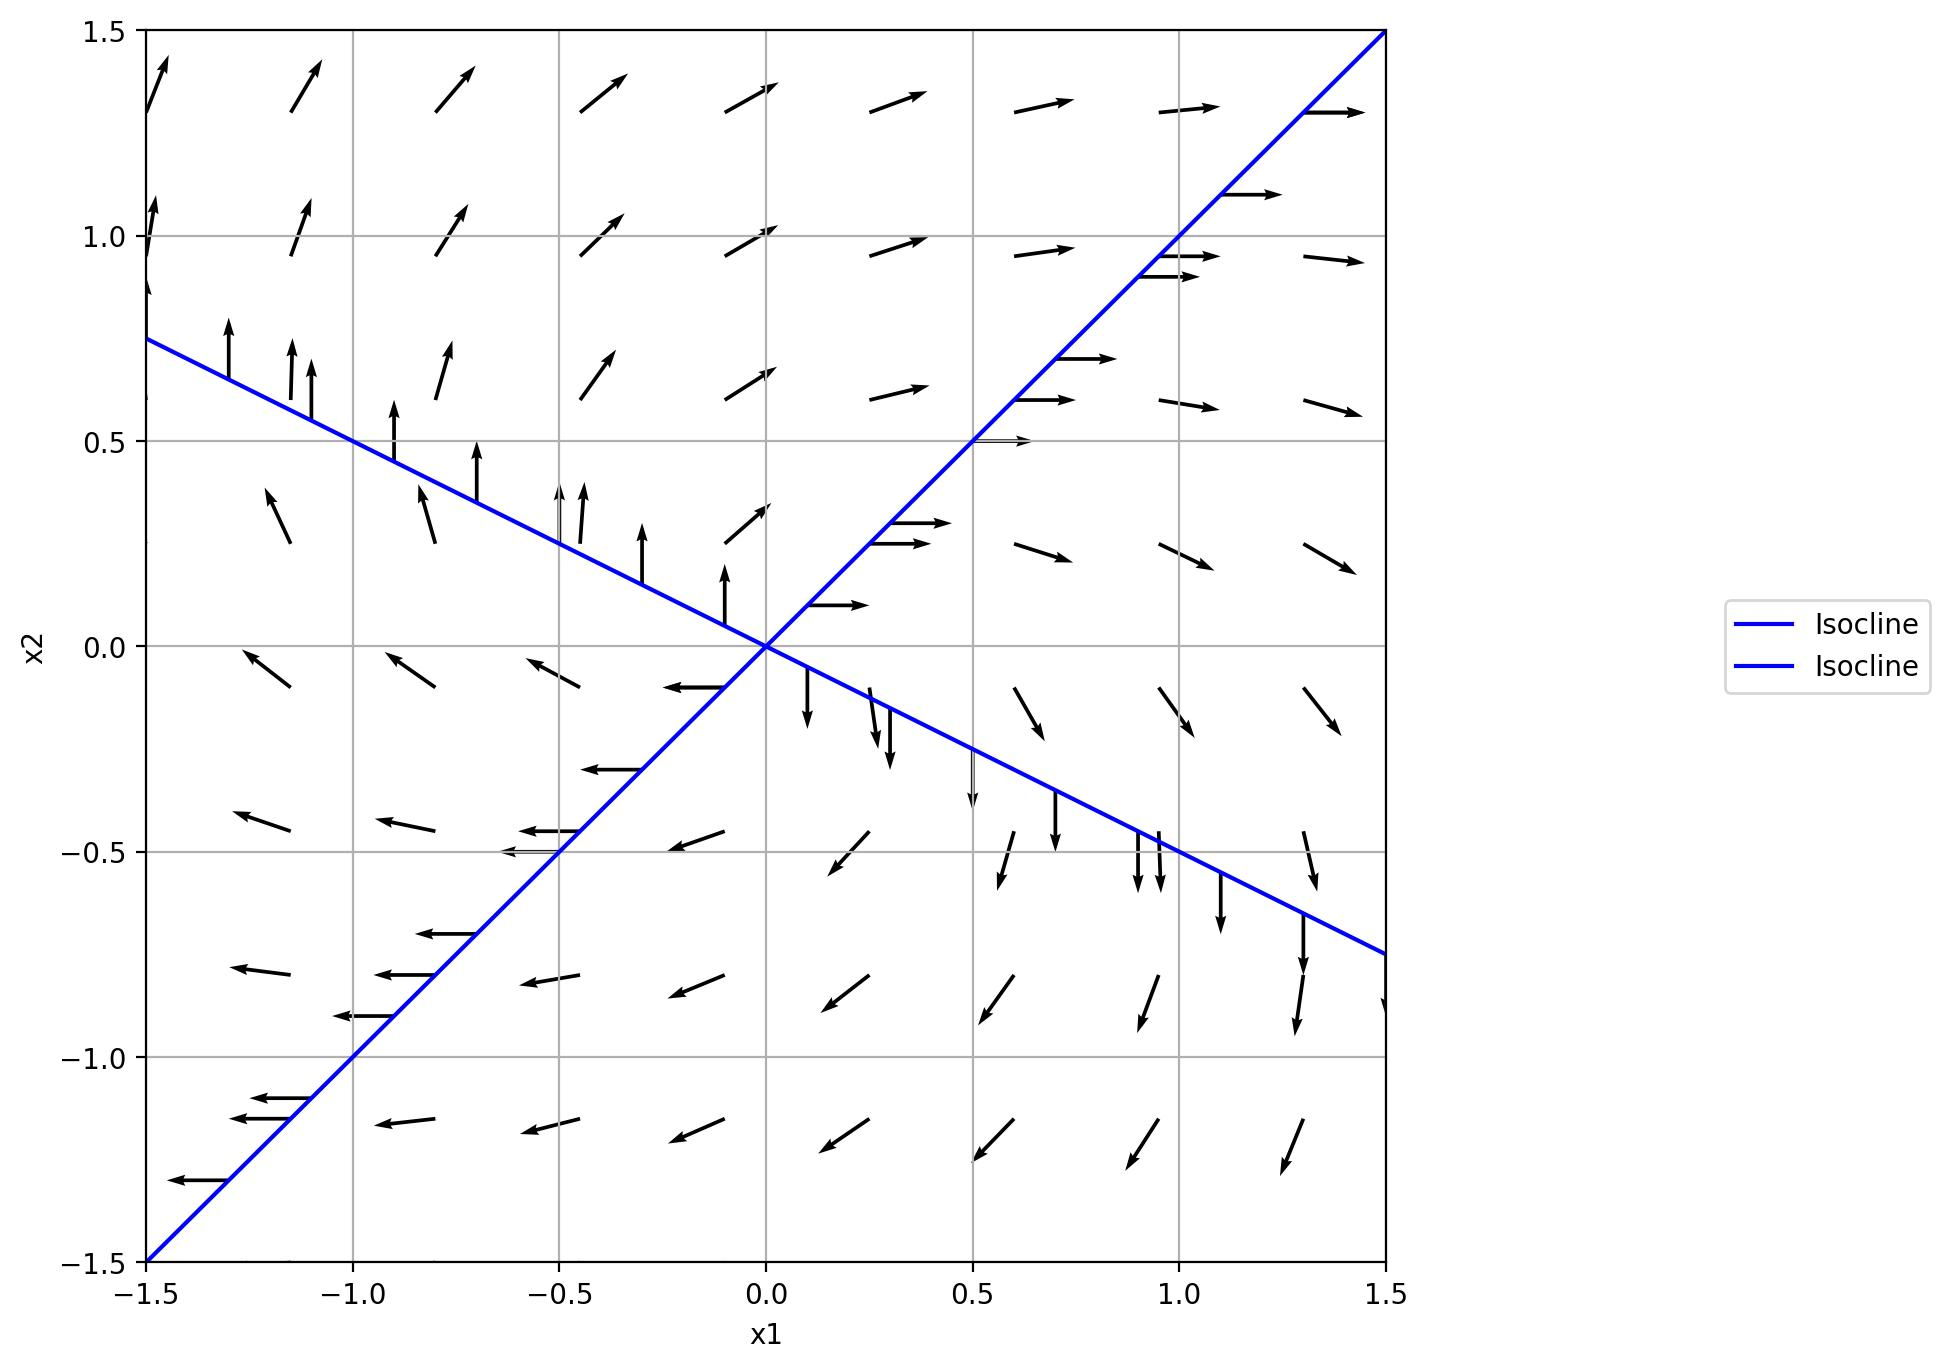
\includegraphics[width=\textwidth]{images/isoclines.jpg}
            \caption{Exemple de portrait de phases avec isoclines et vecteurs vitesse.}
            \label{fig:isoclines}
        \end{figure}
            
    \section{Démarche générale}
        \subsection{Calcul de la trace et du déterminant de la matrice}
        Pour classifier le système selon le diagramme de Poincaré, nous commençons par calculer la trace $\Tr(A)$ et le déterminant $\det(A)$ de la matrice $A$. La trace et le déterminant caractérisent les propriétés dynamiques du système. En les situant sur le diagramme de Poincaré, nous pouvons prédire la nature des points d'équilibre : nœud, foyer, centre, ou selle. Ces informations préliminaires nous orientent vers une première classification du comportement du système.

        \subsection{Calcul des valeurs propres}
            Les valeurs propres $\lambda_1$ et $\lambda_2$ de $A$ sont obtenues en résolvant l'équation caractéristique, ou en résolvant le système \ref{eq:valeurs_propres}. Les solutions de cette équation, $\lambda_1$ et $\lambda_2$, nous permettent d'affiner l’analyse de la stabilité et de déterminer la nature des trajectoires du système. En particulier, la présence de valeurs propres réelles ou complexes, ainsi que le signe de leur partie réelle, dicte si les trajectoires convergent vers l’origine, s’en éloignent ou oscillent autour.
            
        \subsection{Calcul des vecteurs propres et détermination des droites invariantes}
            Les vecteurs propres du système fournissent des informations sur les directions invariantes, c'est-à-dire les trajectoires dans lesquelles la direction ne change pas. Si les valeurs propres sont réelles et distinctes, les vecteurs propres définissent les directions vers lesquelles les trajectoires s’alignent asymptotiquement.
            Ces vecteurs propres permettent de définir des axes de symétrie ou des \textit{droites invariantes} le long desquelles les trajectoires évoluent de manière stable ou instable, selon le signe des valeurs propres associées.

        \subsection{Calcul des isoclines et analyse des signes des dérivées}
            Les isoclines sont les courbes dans le plan sur lesquelles l'une des dérivées est nulle. Sur les isoclines, les vecteurs vitesse sont alignés horizontalement ou verticalement, fournissant une information précieuse sur la direction générale des trajectoires.

        \subsection{Dessin des vecteurs vitesse}
            En traçant les vecteurs vitesse en différents points du plan, nous visualisons le flux du champ de vecteurs. Ce tracé constitue une aide graphique pour comprendre la dynamique du système dans chaque région définie par les isoclines, facilitant l’interprétation des directions dans lesquelles les trajectoires évoluent.

        \subsection{Tracé qualitatif des trajectoires}
        Pour esquisser les trajectoires de manière qualitative, certaines règles sont d'application:
        \begin{enumerate}
            \item Une et une seule trajectoire passe par chaque point du plan, de sorte qu'aucun croisement de trajectoires n'est possible, assurant la cohérence du portrait de phase\footnote{Sinon, le système ne serait pas déterministe.}.
            \item Le signe des dérivées dans chaque région définie par les isoclines permet de déterminer la direction générale des trajectoires, en fonction de le valeur des dérivées $\dot{x}_1$ et $\dot{x}_2$.
            \item Les vecteurs propres déterminent la direction asymptotique de chaque trajectoire vers (ou loin de) l'origine, selon les valeurs propres du système.
        \end{enumerate}

    \section{Exercices conclusifs}
        Appliquez la démarche générale pour les trois systèmes suivants:
        \subsection{Exercice 1}
            \begin{equation*}
                \begin{cases}
                    \dot{x}_1(t) = 2 x_1(t) + x_2(t)\\
                    \dot{x}_2(t) = x_1(t) + 2 x_2(t)
                \end{cases}
            \end{equation*}
            La solution numérique, à titre indicatif, est donnée en figure \ref{fig:conclusif_1}.
            \begin{figure}[ht!]
                \centering
                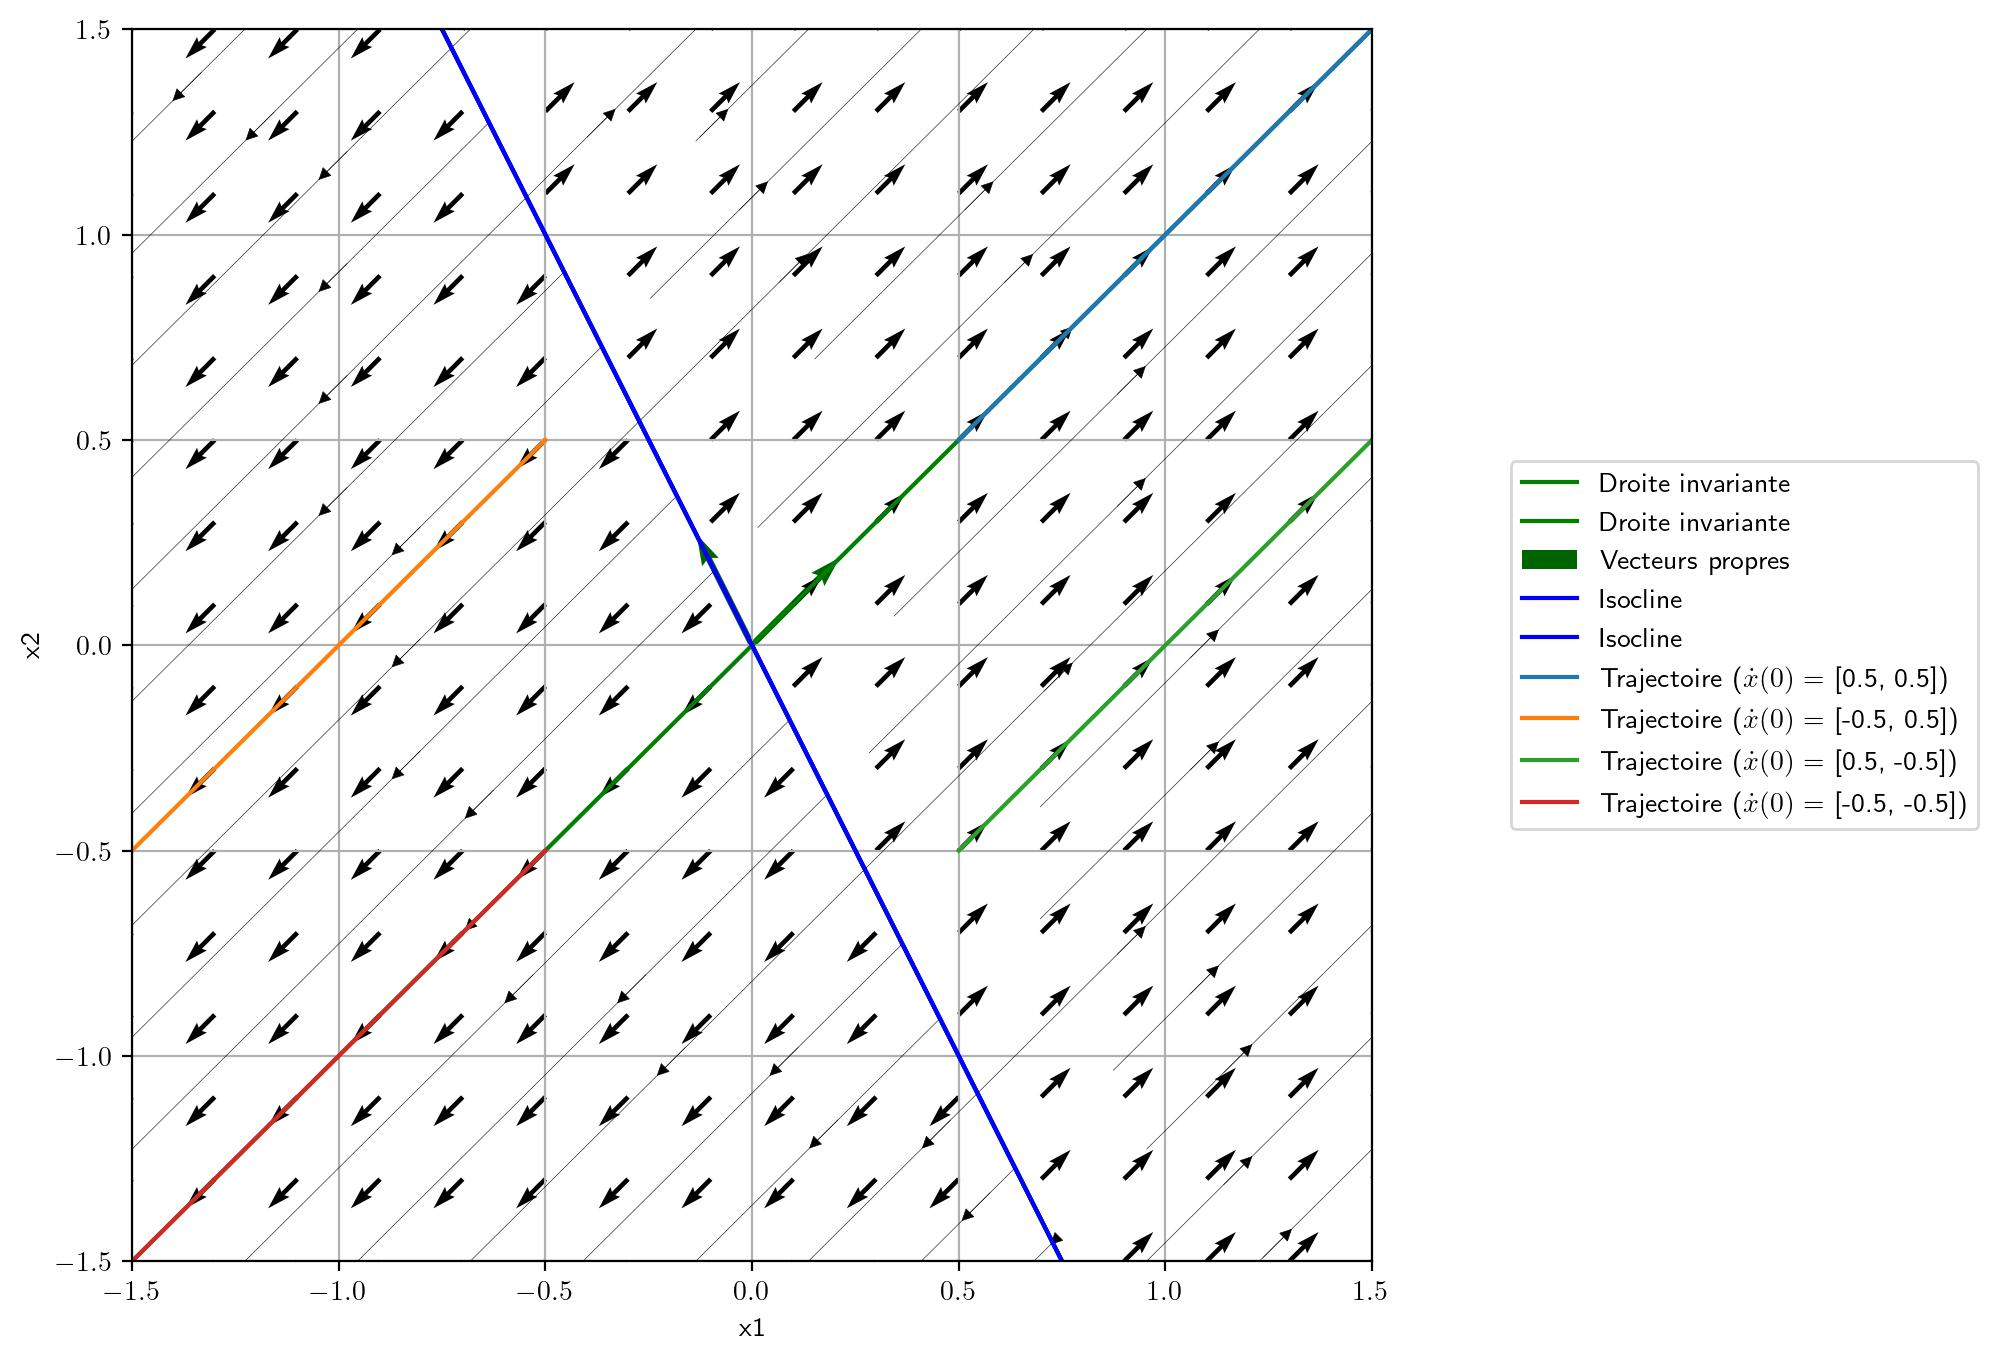
\includegraphics[width=\textwidth]{images/conclusif_1.jpg}
                \caption{Solution de l'exercice 1}
                \label{fig:conclusif_1}
            \end{figure}
        \subsection{Exercice 2}
            \begin{equation*}
                \begin{cases}
                    \dot{x}_1(t) = - x_1(t) - x_2(t)\\
                    \dot{x}_2(t) = x_1(t) - x_2(t)
                \end{cases}
            \end{equation*}
            La solution numérique, à titre indicatif, est donnée en figure \ref{fig:conclusif_2}.
            \begin{figure}[ht!]
                \centering
                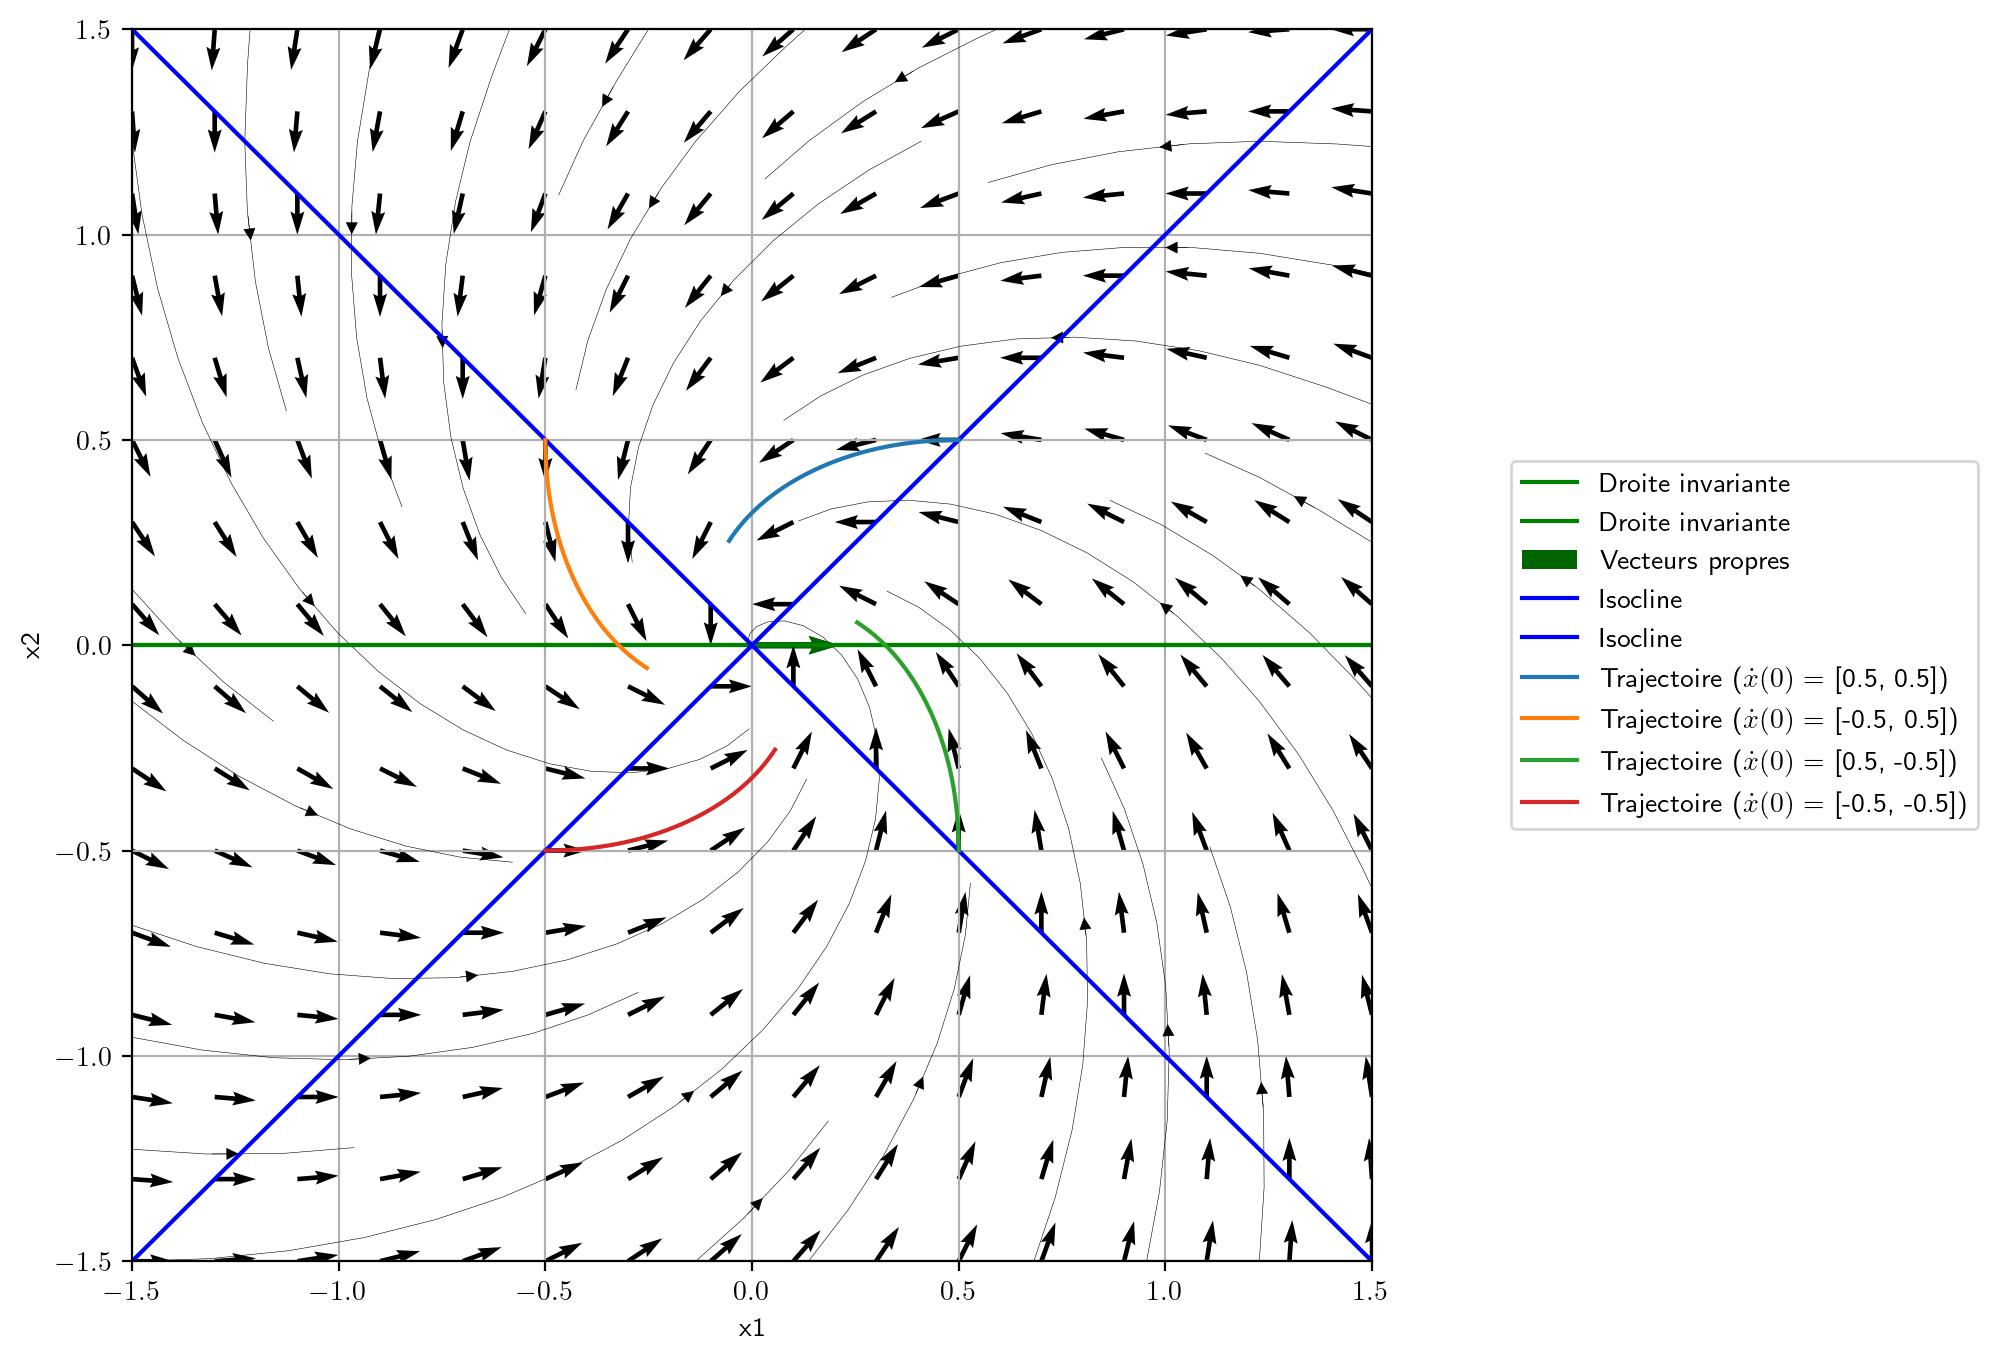
\includegraphics[width=\textwidth]{images/conclusif_2.jpg}
                \caption{Solution de l'exercice 2}
                \label{fig:conclusif_2}
            \end{figure}
        \subsection{Exercice 3}
            \begin{equation*}
                \begin{cases}
                    \dot{x}_1(t) = -2 x_1(t)\\
                    \dot{x}_2(t) = 4 x_1(t) - 2 x_2(t)
                \end{cases}
            \end{equation*}
            La solution numérique, à titre indicatif, est donnée en figure \ref{fig:conclusif_3}.
            \begin{figure}[ht!]
                \centering
                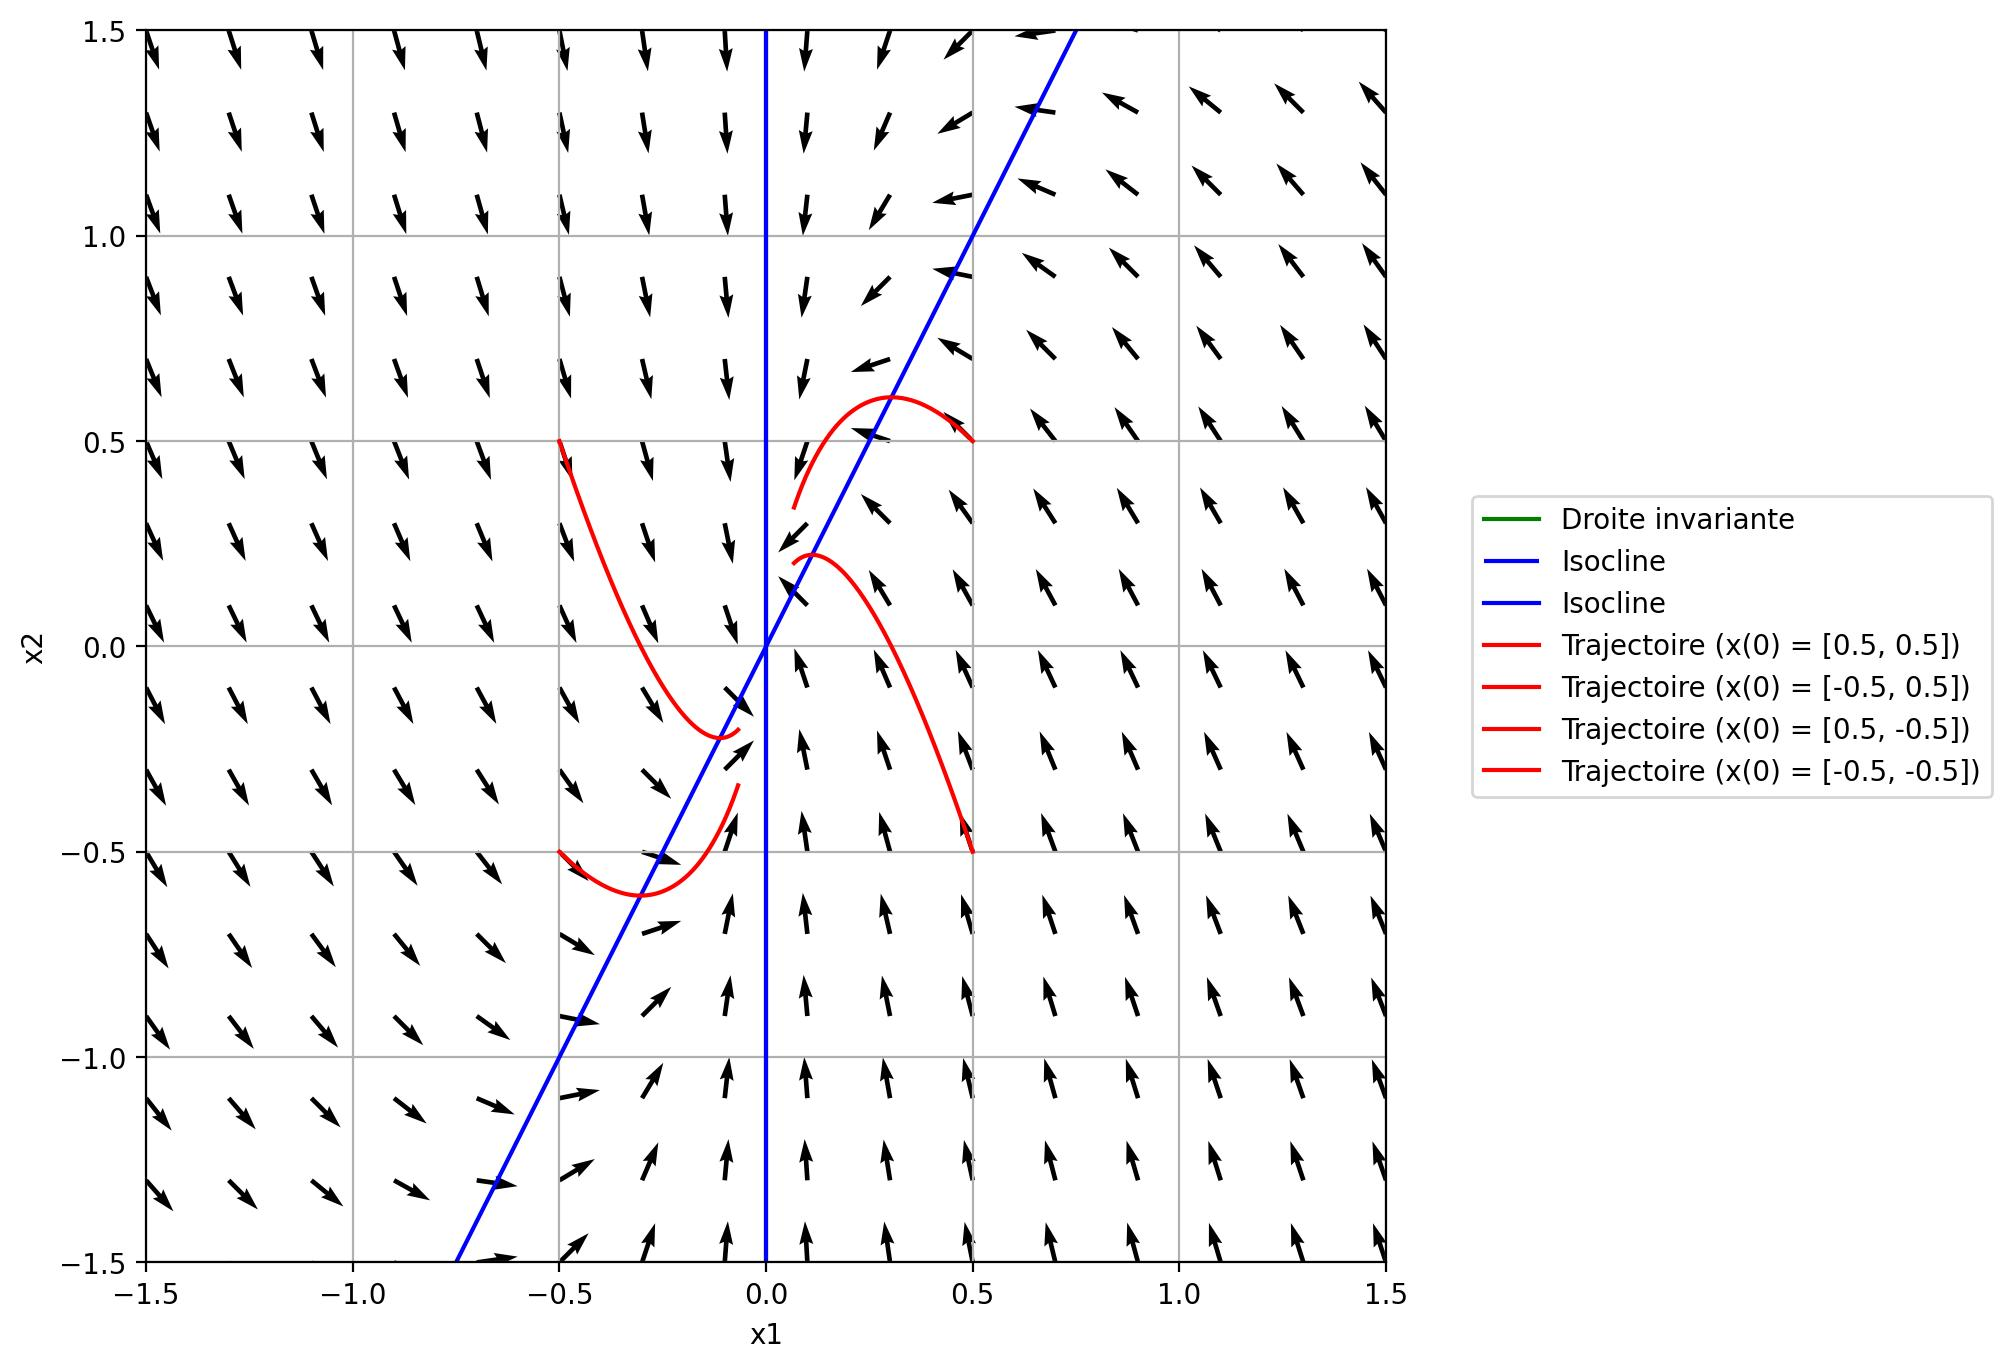
\includegraphics[width=\textwidth]{images/conclusif_3.jpg}
                \caption{Solution de l'exercice 3}
                \label{fig:conclusif_3}
            \end{figure}
\chapter{Portraits de phases de systèmes non-linéaires}
    \section{Introduction}
    \section{Systèmes non-linéaires d'ordre 2}
        Soit un système dynamique non-linéaire défini par le système d'équations différentielles :
        \begin{equation}
            \begin{cases}
                \dot{x}_1 = f_1(x_1, x_2) \\
                \dot{x}_2 = f_2(x_1, x_2)
            \end{cases}
        \end{equation}
        où au moins une des fonctions $f_1$ ou $f_2$ est non linéaire. Dans le cas de systèmes non linéaires, l'analyse directe peut être complexe, voire impossible. Cependant, une approche standard pour comprendre le comportement local du système autour d'un point d'équilibre consiste à linéariser le système. Cette méthode s'appuie sur le développement de la fonction au voisinage de points spécifiques (typiquement des points d'équilibre) et permet d'extraire des informations cruciales sur la dynamique locale.

        Pour réaliser cette approximation linéaire, pour autant que $f_1$ et $f_2$ sont dérivables, nous calculons la \textit{matrice jacobienne} du système, qui décrit la variation infinitésimale des fonctions $f_1$ et $f_2$ par rapport aux variables $x_1$ et $x_2$. Renvoyons bien entendu l'étudiant·e au cours de Mathématiques pour une définition formelle de la dérivabilité (\cite{mathf117}). La matrice jacobienne s'exprime comme suit :

        \begin{definition}{Matrice jacobienne}
            La matrice jacobienne d'un système est définie comme la matrice des dérivées partielles selon les composantes. Dans le cas d'ordre 2,
            \begin{equation}
                J = 
                \begin{bmatrix}
                    \pd {f_1}{x_1} & \pd {f_1}{x_2} \\
                    \pd {f_2}{x_1} & \pd {f_2}{x_2}
                \end{bmatrix}
            \end{equation}
        \end{definition}
        L'évaluation de cette matrice au point d'équilibre (en posant $\dot{x}_1 = \dot{x}_2 = 0$) fournit un système linéarisé, dont le comportement global autour de l'équilibre peut être interprété en analysant les valeurs propres de $J$.

        Les valeurs propres de cette matrice jacobienne jouent un rôle crucial dans la classification locale du point d'équilibre en tant que nœud, foyer, point-selle, ou centre :
        \begin{itemize}
            \item si les valeurs propres sont réelles et de même signe, le point d'équilibre est un nœud attractif ou répulsif~;
            \item si les valeurs propres sont réelles et de signes opposés, le point d'équilibre est un point-selle, indiquant un comportement divergent sur certaines directions et convergent sur d'autres~;
            \item si les valeurs propres sont complexes conjuguées avec une partie réelle non nulle, le point est un foyer, décrivant un comportement oscillatoire autour de l'équilibre~;
            \item si les valeurs propres sont purement imaginaires, le point d'équilibre est un centre, et le système suit des trajectoires fermées autour de ce point.
        \end{itemize}
        Notons que cette classification est uniquement valide si les valeurs propres de $J$ sont toutes deux non nulles, assurant que le point d'équilibre est non dégénéré.

        \subsection{Calcul des isoclines}
            Le calcul des isoclines d'un système non-linéaire se fait de manière analogue à celle des cas linéaire. La définition d'une isocline (voir \ref{def:isocline}) reste valable: pour calculer les isoclines d'un système, on détermine l'équation obtenue par l'annulation de chacune des dérivées. Prenons par exemple le système
            \begin{equation}\label{eq:isocline_non_lineaire}
                \begin{cases}
                    \dot{x}_1 = x_1^2 + x_2 \\
                    \dot{x}_2 = x_2
                \end{cases}
            \end{equation}

            Nous pouvons en calculer les deux isoclines. Commençons par annuler la première dérivée. L'isocline correspondante est décrite par l'équation $0 = x_1^2 + x_2$, ou $x_2 = -x_1^2$. C'est une équation parabolique négative dont le sommet se trouve à l'origine. La deuxième isocline se calcule de manière similaire, et donne $x_2 = 0$, droite horizontale confondue avec l'axe $x_1$. Dans la figure \ref{fig:exemple_non_lineaire_1}, on montre le portrait de phase associé à ce système.
            \begin{figure}[ht!]
                \centering
                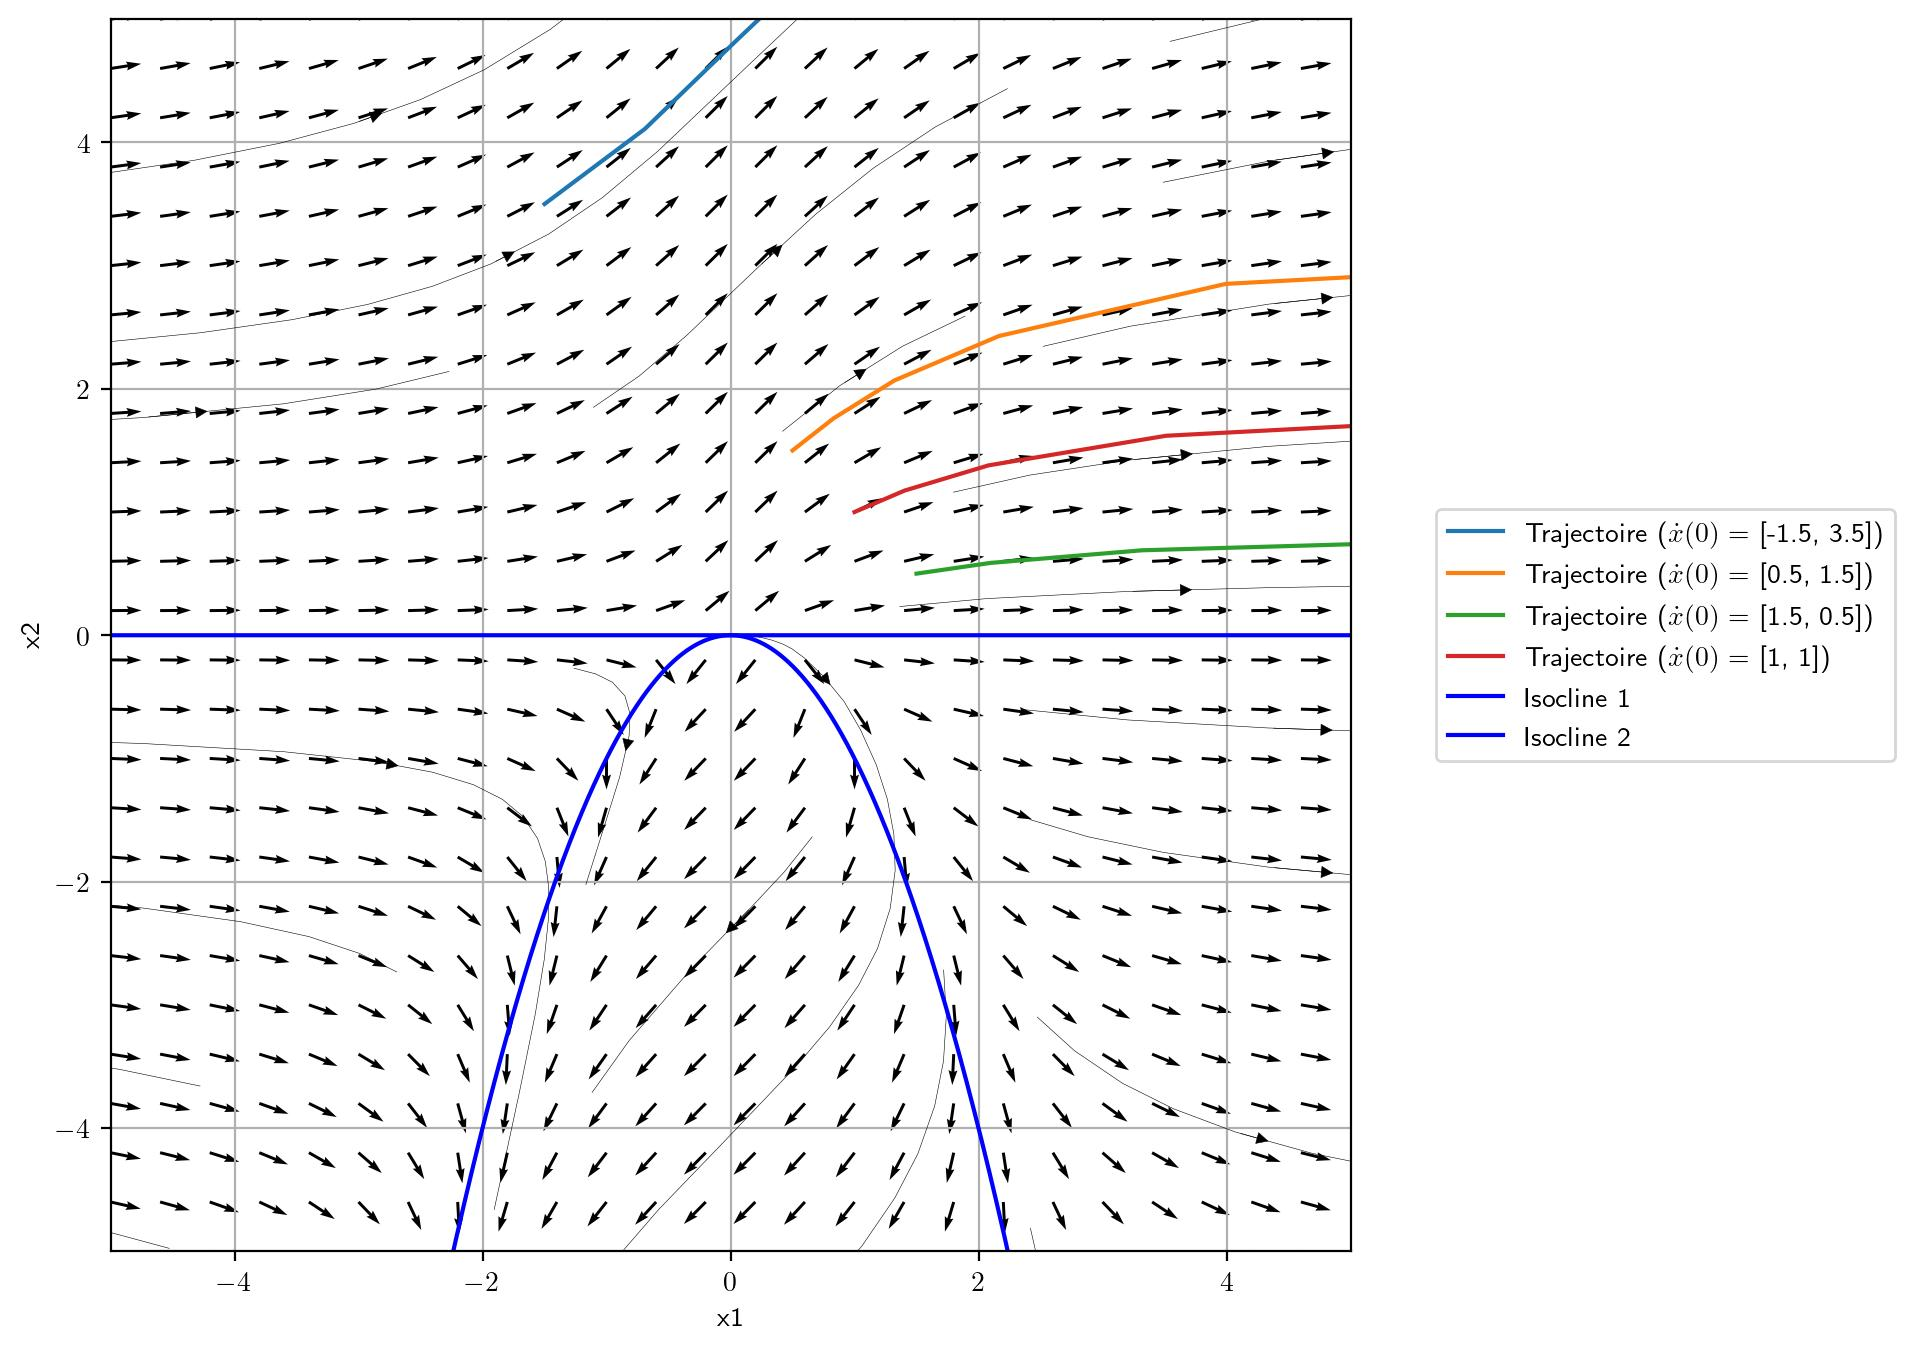
\includegraphics[width=\textwidth]{images/exemple_non_lineaire_1.jpg}
                \caption{Portrait de phase du système \ref{eq:isocline_non_lineaire}. Les deux isoclines sont marquées en bleu.}
                \label{fig:exemple_non_lineaire_1}
            \end{figure}

        \subsection{Calcul des points d'équilibre}
            Ici encore, la définition donnée en \ref{def:point_equilibre} reste valable: les points d'équilibres sont les points pour lesquels la variation est nulle (c'est à dire, où les deux dérivées sont annulées en même temps). Par définition, les points d'équilibre correspondent aux points d'intersection entre les isoclines.
            Prenons le système
            \begin{equation}\label{eq:equilibre_non_lineaire}
                \begin{cases}
                    \dot{x}_1 = x_1 \\
                    \dot{x}_2 = \sin{x_2}
                \end{cases}
            \end{equation}
            Calculer le (les) point(s) d'équilibre revient à résoudre le système
            \begin{equation}
                \begin{cases}
                    0 = x_1 \\
                    0 = \sin{x_2}
                \end{cases}
            \end{equation}
            Les points d'équilibre sont donc situés sur la droite d'équation $x_1 = 0$, là ou $\sin x_2 = 0$. La figure \ref{fig:equilibre_non_lineaire_2} montre le portrait de phase associé au système \ref{eq:equilibre_non_lineaire} et en montre les points d'équilibre.
            \begin{figure}[ht!]
                \centering
                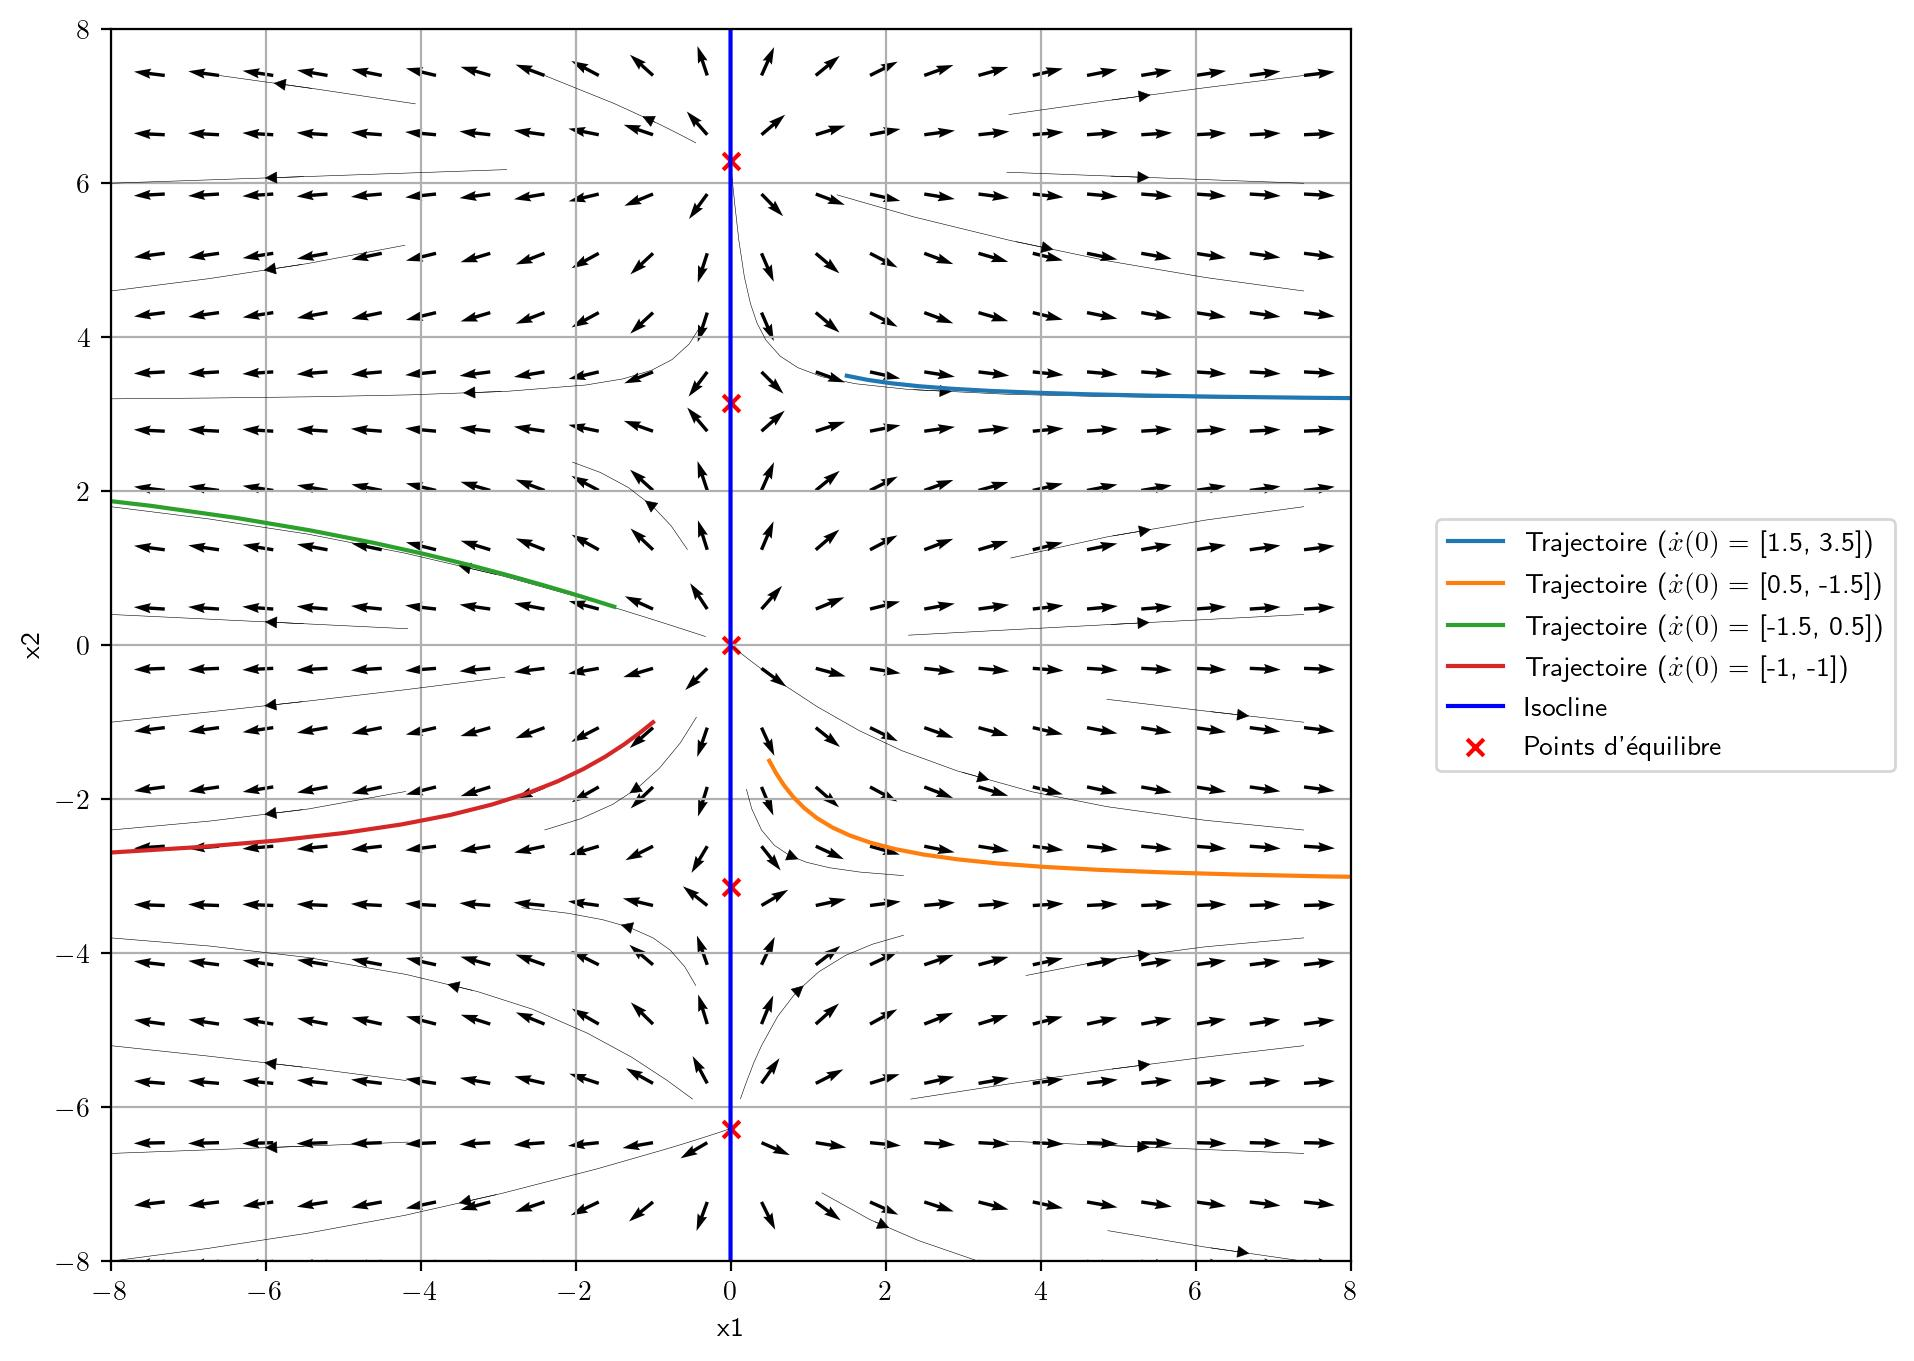
\includegraphics[width=\textwidth]{images/exemple_non_lineaire_2.jpg}
                \caption{Portrait de phase du système \ref{eq:equilibre_non_lineaire}. Les points d'équilibre sont marqués par des croix rouges.}
                \label{fig:equilibre_non_lineaire_2}
            \end{figure}
            
        \subsection{Stabilité des points d'équilibre}
            Le système précédent met en avant un phénomène déjà étudié dans le cadre des systèmes linéaires, celui de \textit{stabilité}. 
            Autour des différents points d'équilibre montrés sur dans la figure \ref{fig:equilibre_non_lineaire_2}, les trajectoires et les vecteurs vitesse s'éloignent, montrant qu'une condition initiale proche du point d'équilibre aura tendance à mener à une trajectoire divergente de ce point. Ces points d'équilibres sont donc \textit{instables}. Formellement, les définitions données en \ref{def:stabilite} restent valables dans le contexte non-linéaire, bien que leur vérification puisse demander des calculs plus fastidieux. En effet, comme expliqué dans le syllabus (\cite{infof305}), la vérification de la stabilité des points d'équilibre peut être réalisée en étudiant les \textit{critères de stabilité de Lyapounov\footnote{Alexandre Lyapounov (en russe, Александр Михайлович Ляпунов est un mathématicien russe né en 1857 et mort de sa propre main en 1918. Ses contributions majeurs concernent l'étude de la stabilité des systèmes dynamiques. Ce sujet vaste trouve ses balbutiements au 17ème siècle, avec des mathématiciens comme Evangelisto Torricelli et Galileo Galilei.}} (\cite{lyapounov}). 

            Pour rappel: soit un système à temps continu décrit par $\dot{x}(t) = f(x(t), u(t))$, où $f(\cdot, \cdot)$ et ses dérivées partielles sont connues. Admettons que nous ayons déjà calculé les points d'équilibre, comme expliquée dans la section précédente, et soit un point d'équilibre $\bar{x}$. Lyapounov nous dit que si il existe une fonction $V(\cdot)$ continue, ainsi que ses dérivées partielles, qui est définie positive en $\bar{x}$ et telle que la fonction 
            \begin{equation}
                \dot{V}(x(t)) = \frac{\dd V(x(t))}{\dd t} = \nabla V(x)f(x, \bar u)
            \end{equation}
            où $\nabla V(x) = [\frac{\dd V}{\dd x_1}, \frac{\dd V}{\dd x_2}, ..., \frac{\dd V}{\dd x_n}]$, est semi-définie négative en $\bar x$ alors $\bar x$ est un état d'équilibre \textit{stable}. Si cette même fonction est définie négative, alors l'équilibre est \textit{asymptotiquement stable}.

            Afin de rendre ces définitions plus claires, reprenons le système \ref{eq:equilibre_non_lineaire} en exemple:
            \begin{equation}
                \begin{cases}
                    \dot{x}_1 = x_1 \\
                    \dot{x}_2 = \sin{x_2}
                \end{cases}
            \end{equation}
            Nous avons déjà calculé ses points d'équilibre, prenons l'origine comme cas étudié ici.

            Prenons une fonction de Lyapounov candidate (et effectivement définie positive:
            \begin{equation}
                V(x_1, x_2) = \frac12 x_1^2 + \frac12 x_2^2 + 1
            \end{equation}
            Son gradient le long des trajectoires du système est donné par 
            \begin{equation}
                \dot V(x_1, x_2) = x_1x_1 + x_2\sin x_2 = x_1^2 + x_2\sin x_2
            \end{equation}
            Étudions le signe de cette fonction. Le premier terme, $x_1^2$ est positif ou nul. Rappelons que le point d'équilibre est à l'origine. Si $x_2$ est (donc légèrement) négatif, son sinus l'est aussi, et le deuxième terme est positif. Si $x_2$ est légèrement positif, son sinus l'est aussi et le deuxième terme est aussi positif. Le résultat de cette expression est donc positif dans le voisinage du point d'équilibre. Si l'on reprend le critère de Lyapounov, il en résulte que $V(\cdot)$ n'est ni définie négative, ni semi-définie négative, donc le système n'est pas stable. En se référant à la définition d'instabilité du syllabus, on en déduit que le système est instable autour de ce point d'équilibre. Observons à nouveaux le portrait de phase donné en figure \ref{fig:equilibre_non_lineaire_2}. Le point d'équilibre à l'origine semble en effet instable.
            
    \section{Exercices}
        L’objectif est de mener une analyse complète de ces systèmes en plusieurs étapes, qui sont détaillées ci-dessous. Cette analyse permettra d’examiner la dynamique des solutions dans le plan de phase et d’approfondir notre compréhension des comportements locaux autour des points d'équilibre.
    
        \begin{enumerate}
            \item Calcul et tracé des isoclines.
            \item Détermination des points d'équilibre
            \item Calcul de la matrice jacobienne. Le calcul de $J$ pour chacun des systèmes aux points d’équilibre permet d'obtenir une approximation linéaire du comportement du système autour de ces points.
            \item Étude du comportement local avec la matrice jacobienne: au voisinage de chaque point d’équilibre, nous utilisons la matrice jacobienne pour analyser la stabilité locale, comme vu durant ce chapitre. En examinant les valeurs propres de cette matrice, nous déterminons la nature du point d'équilibre (nœud, foyer, point-selle, etc.) et décrivons le comportement local des trajectoires.
            \item Dessin du portrait de phase.
            \item Étude analytique, par une fonction de Lyapounov bien choisie, de la stabilité des points d'équilibre, comme montré dans ce chapitre.
            
        
        \end{enumerate}
        Cette démarche permet une compréhension approfondie de chaque système dynamique, tant au niveau local qu’au niveau global, en combinant linéarisation locale et analyse graphique pour obtenir une interprétation complète des trajectoires et des comportements des solutions.

        \subsection{Exercice 1}
            \begin{exercise}{Exercice 1}
                \begin{equation}
                    \begin{cases}
                        \dot{x}_1 = x_1 \\
                        \dot{x}_2 = x_1^2 + x_2^2 - 1
                    \end{cases}
                \end{equation}
            \end{exercise}
            La solution numérique est donnée à titre indicatif dans la figure \ref{fig:pdp_exercice_3_1}.
            \begin{figure}[ht!]
                \centering
                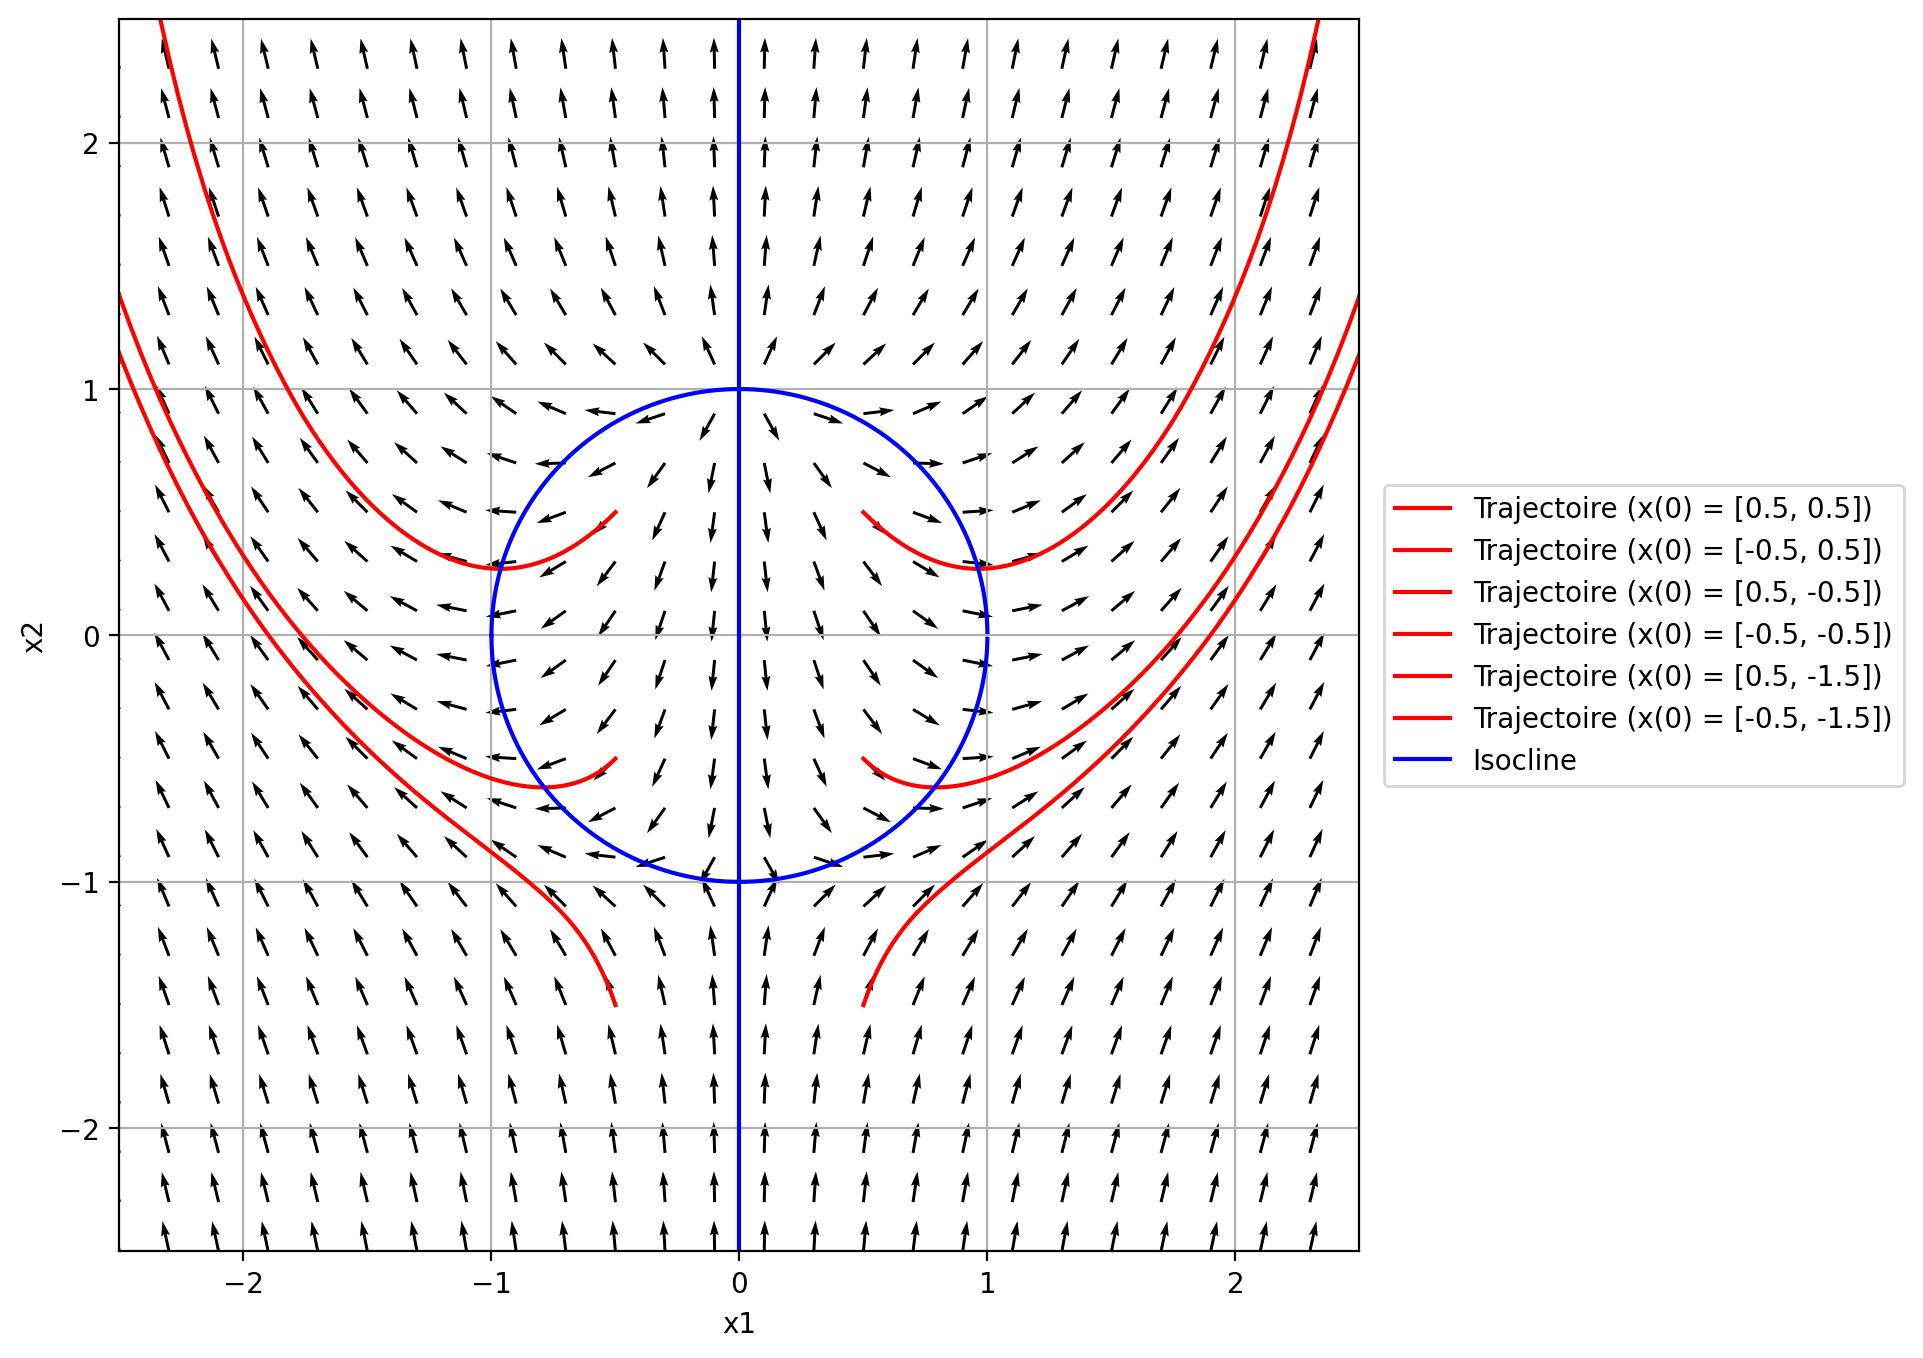
\includegraphics[width=\textwidth]{images/pdp_exercice_3_1.jpg}
                \caption{Solution numérique de l'exercice 1}
                \label{fig:pdp_exercice_3_1}
            \end{figure}
            
        \subsection{Exercice 2}
            \begin{exercise}{Exercice 2}
                \begin{equation}
                    \begin{cases}
                        \dot{x}_1 = x_2 \\
                        \dot{x}_2 = x_1(1 - x_1^2) + x_2
                    \end{cases}
                \end{equation}
            \end{exercise}
            La solution numérique est donnée à titre indicatif dans la figure \ref{fig:pdp_exercice_3_2}.
            \begin{figure}[ht!]
                \centering
                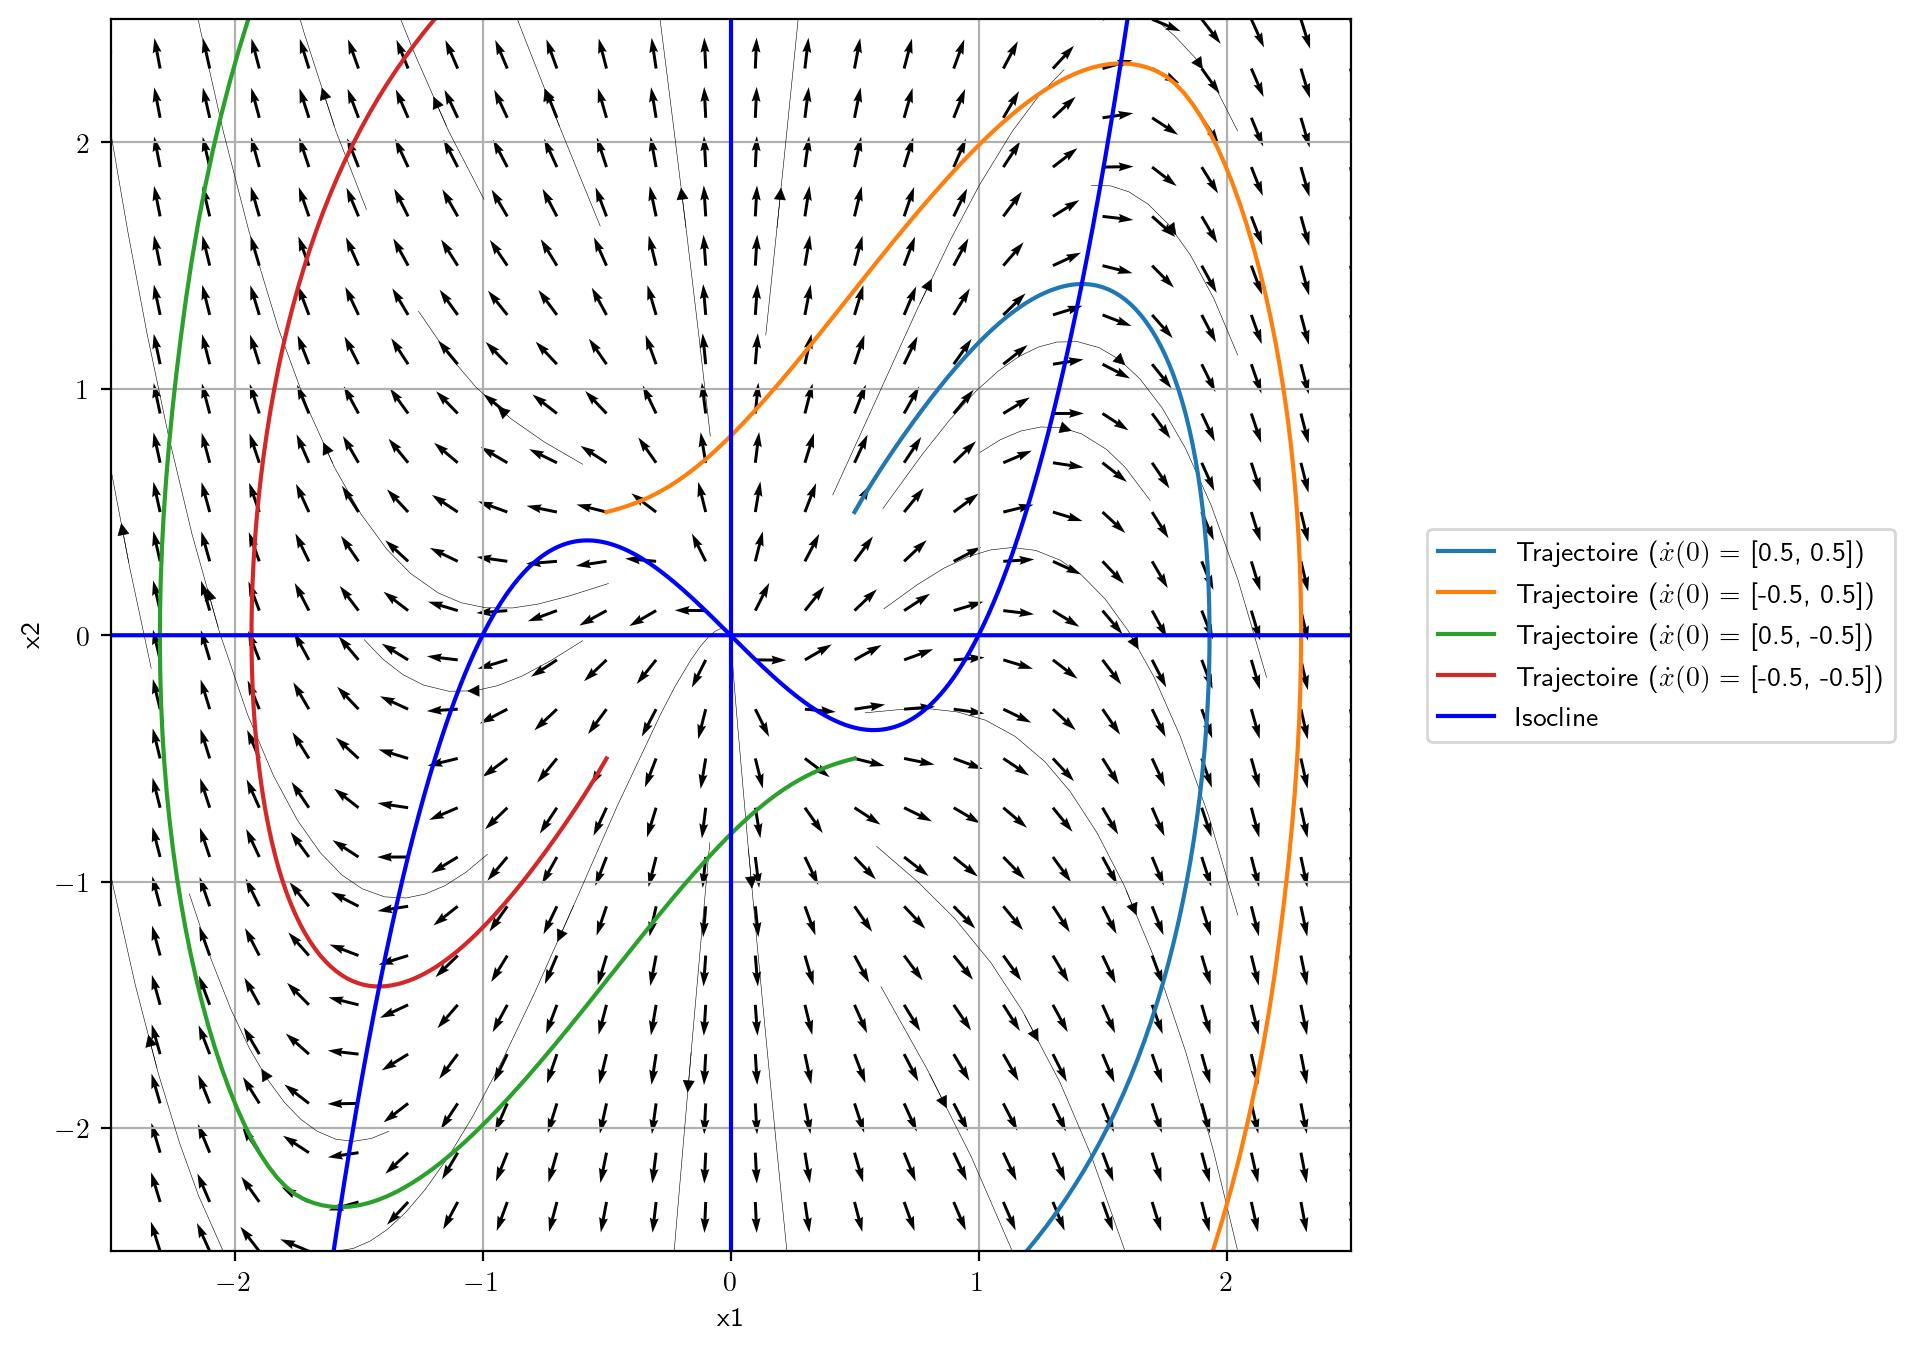
\includegraphics[width=\textwidth]{images/pdp_exercice_3_2.jpg}
                \caption{Solution numérique de l'exercice 2}
                \label{fig:pdp_exercice_3_2}
            \end{figure}

        \subsection{Exercice 3}
            \begin{exercise}{Exercice 3}
                \begin{equation}
                    \begin{cases}
                        \dot{x}_1 = 0.2 x_1 - 0.08 x_1 x_2 \\
                        \dot{x}_2 = 0.1 x_1 x_2 - 0.2 x_2
                    \end{cases}
                \end{equation}
            \end{exercise}
            La solution numérique est donnée à titre indicatif dans la figure \ref{fig:pdp_exercice_3_3}.
            \begin{figure}[ht!]
                \centering
                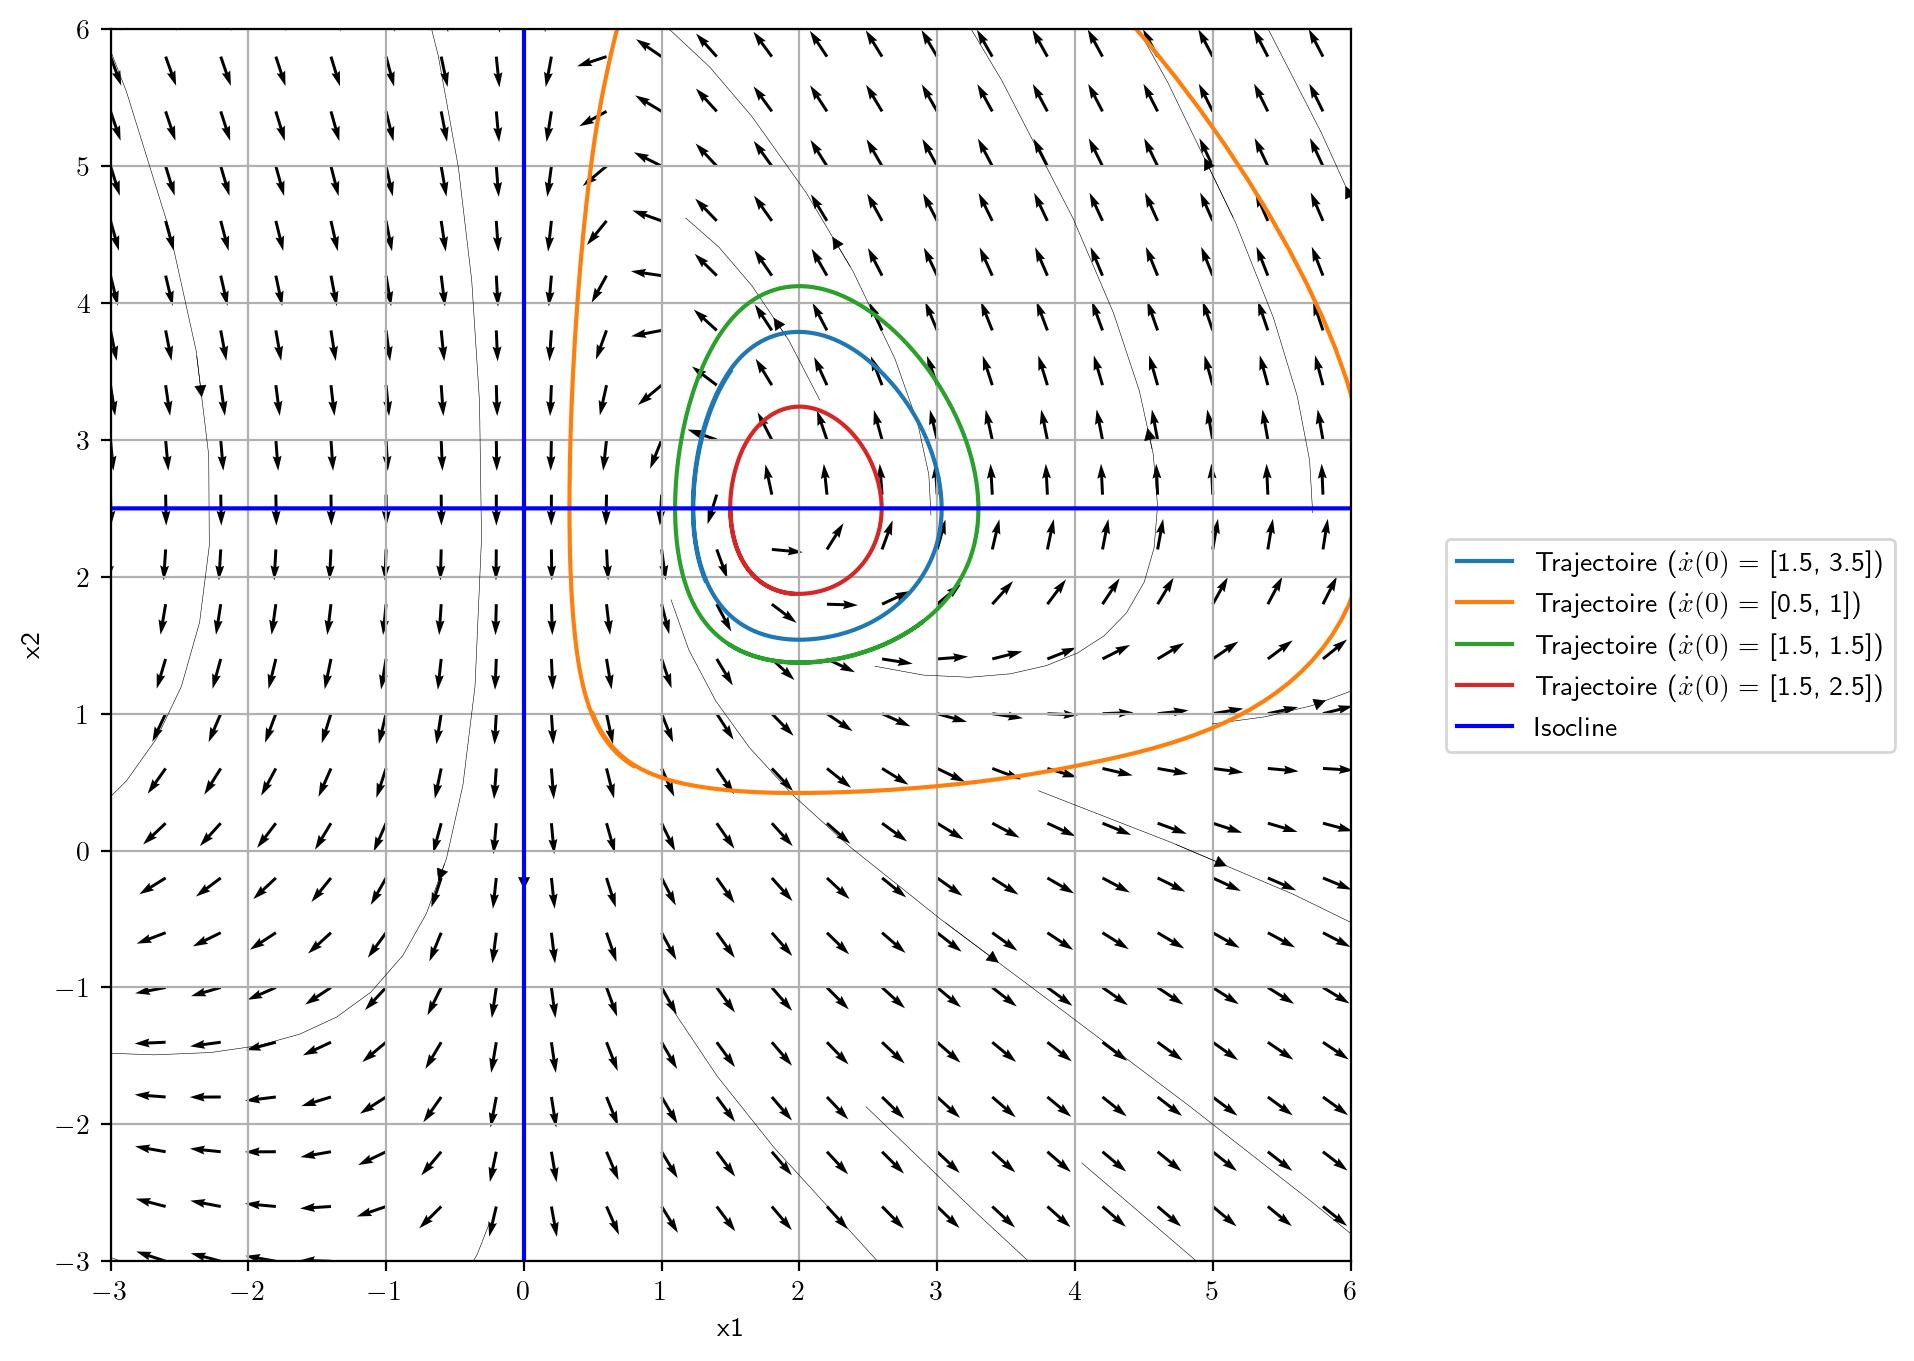
\includegraphics[width=\textwidth]{images/pdp_exercice_3_3.jpg}
                \caption{Solution numérique de l'exercice 3}
                \label{fig:pdp_exercice_3_3}
            \end{figure}

\chapter{Simulation numérique}

    \section{Introduction}
    La simulation numérique repose sur des outils mathématiques et algorithmiques pour transformer des équations différentielles en solutions approchées, fournissant ainsi un aperçu précieux sur des systèmes temporels. Ce chapitre introduit deux bibliothèques Python incontournables pour le calcul scientifique et la résolution numérique: \codeword{Numpy} pour la manipulation efficace des données et \codeword{SciPy} pour l'intégration numérique et la résolution de systèmes dynamiques.

    \section{Introduction à \texttt{Numpy}}
        \codeword{Numpy}, abréviation de \textit{Numerical Python}, est une bibliothèque qui s'est imposée dans le domaine du calcul scientifique (\cite{Numpy2020}). Elle propose des structures de données optimisées et un riche ensemble de fonctions mathématiques, rendant les manipulations et les calculs de tableaux multidimensionnels performants, en s'appuyant sur la notion de parallélisation. 

        \subsection{Pourquoi utiliser \texttt{Numpy} ?}
            L'un des principaux attraits de \codeword{Numpy} réside dans son efficacité. Les tableaux \codeword{Numpy} (appelés \codeword{ndarrays}) surpassent largement les listes natives de Python en termes de performance, en particulier pour la manipulation de grands ensembles de données. Cette performance est le fruit d'une implémentation sous-jacente en \codeword{C}, permettant à \codeword{Numpy} de bénéficier de la puissance du calcul vectorisé. Le calcul vectorisé, au lieu de traiter les éléments un par un, applique des opérations sur l'ensemble des éléments d'un tableau en une seule commande. En évitant les boucles explicites, \codeword{Numpy} offre un gain de vitesse significatif et rend le code plus lisible et compact.

        \subsection{Comment utiliser \texttt{Numpy} ?}
            Pour exploiter pleinement le potentiel de \codeword{Numpy}, il est essentiel de comprendre ses principales fonctionnalités. Nous introduisons des exemples pratiques, couvrant la création, la manipulation et l’application de fonctions mathématiques sur les tableaux.

            \subsubsection{Création et manipulation de tableaux}
                La création de tableaux est au cœur de l'utilisation de \codeword{Numpy}. Voici un exemple basique de création et manipulation d'un tableau \codeword{Numpy}:
                \inputminted{python}{codes/np_array.py}

            \subsubsection{Fonctions mathématiques vectorisées}
                \codeword{Numpy} permet l’application simultanée de fonctions mathématiques standards à chaque élément d’un tableau. Ce comportement vectorisé confère aux fonctions mathématiques de \codeword{Numpy} une grande efficacité, comme illustré ci-dessous:
                \inputminted{python}{codes/np_math.py}
            
            \subsubsection{Génération de séquences et nombres aléatoires}
                \codeword{Numpy} propose des fonctions pré-établies pour la génération de séquences arithmétiques et de nombres aléatoires, qui sont des outils précieux pour l'initialisation de simulations:
                \inputminted{python}{codes/np_init.py}
                \inputminted{python}{codes/np_random.py}
            
            \subsubsection{Calcul matriciel et multiplication matricielle}
                En plus de la manipulation de tableaux, \codeword{Numpy} dispose d’outils pour les calculs matriciels:
                \inputminted{python}{codes/np_matrix.py}
                Si la multiplication doit être matricielle:
                \inputminted{python}{codes/np_matmul.py}
    \section{Solveur numérique}
        Pour résoudre les systèmes dynamiques, nous utiliserons la fonction \codeword{solve_ivp} du module \codeword{integrate}, dans la librairie \codeword{SciPy} (\cite{Scipy2020}). Cette fonction intègre numériquement des équations différentielles. \robin{Tu peux faire le lien avec les algorithmes de type Runge-Kutta (fonctionnement par défaut de \texttt{solve\_ivp}) qui sont vus en F205.} Elle prend en paramètres:
        \begin{itemize}
            \item \textbf{La fonction à intégrer} : une fonction Python définissant l’équation différentielle.
            \item \textbf{L'intervalle de simulation} : la durée de la simulation.
            \item \textbf{Les points de discrétisation} : un \codeword{numpy.ndarray} définissant les points temporels pour lesquels la solution sera évaluée.
        \end{itemize}

    \section{Simulation de systèmes d'ordre 1}
        Dans cette section, nous explorerons des exemples classiques de systèmes d'ordre 1, résolus numériquement à l'aide de \codeword{SciPy}. Ces exemples sont plus simples que ceux abordés dans le chapitre \ref{chap:portrait_phases}, mais ils permettent de se familiariser avec la syntaxe qu'imposent \codeword{Numpy} et \codeword{SciPy}.
    
        \subsection{Intégrateur simple}
            Nous commençons par un modèle d'intégrateur simple, décrit par le système suivant \robin{à nouveau $y(t)=x(t)$, je ne comprends pas la notation.} \robin{Utilisation de 'prime' pour une dérivée (temporelle) alors que 'point' était utilisé jusqu'ici.}:
            \begin{equation*}
                \begin{cases}
                    x'(t)=c\,u(t)\\
                    y(t)=x(t)
                \end{cases}
            \end{equation*}
            avec les conditions initiales suivantes :
            \begin{itemize}
                \item Condition initiale: $x(0)=1$,
                \item Valeur du paramètre: $c=1$,
                \item Intervalle temporel: $[0,10]$,
                \item Entrée: $u(t)=\sin(t)$.
            \end{itemize}

            \subsubsection{Solution numérique}
                Le code suivant résout numériquement le système et affiche le résultat via la bibliothèque \codeword{Matplotlib} (\cite{Matplotlib2007}). Le graphique est présenté en Figure \ref{fig:integrateur_simple}. \robin{P-ê mentionner que la solution au système est $x(t) = 2-\cos t$ pour confirmer visuellement la solution~?}
                \inputminted{python}{codes/integrateur_simple.py}
                \begin{figure}[ht!]
                    \centering
                    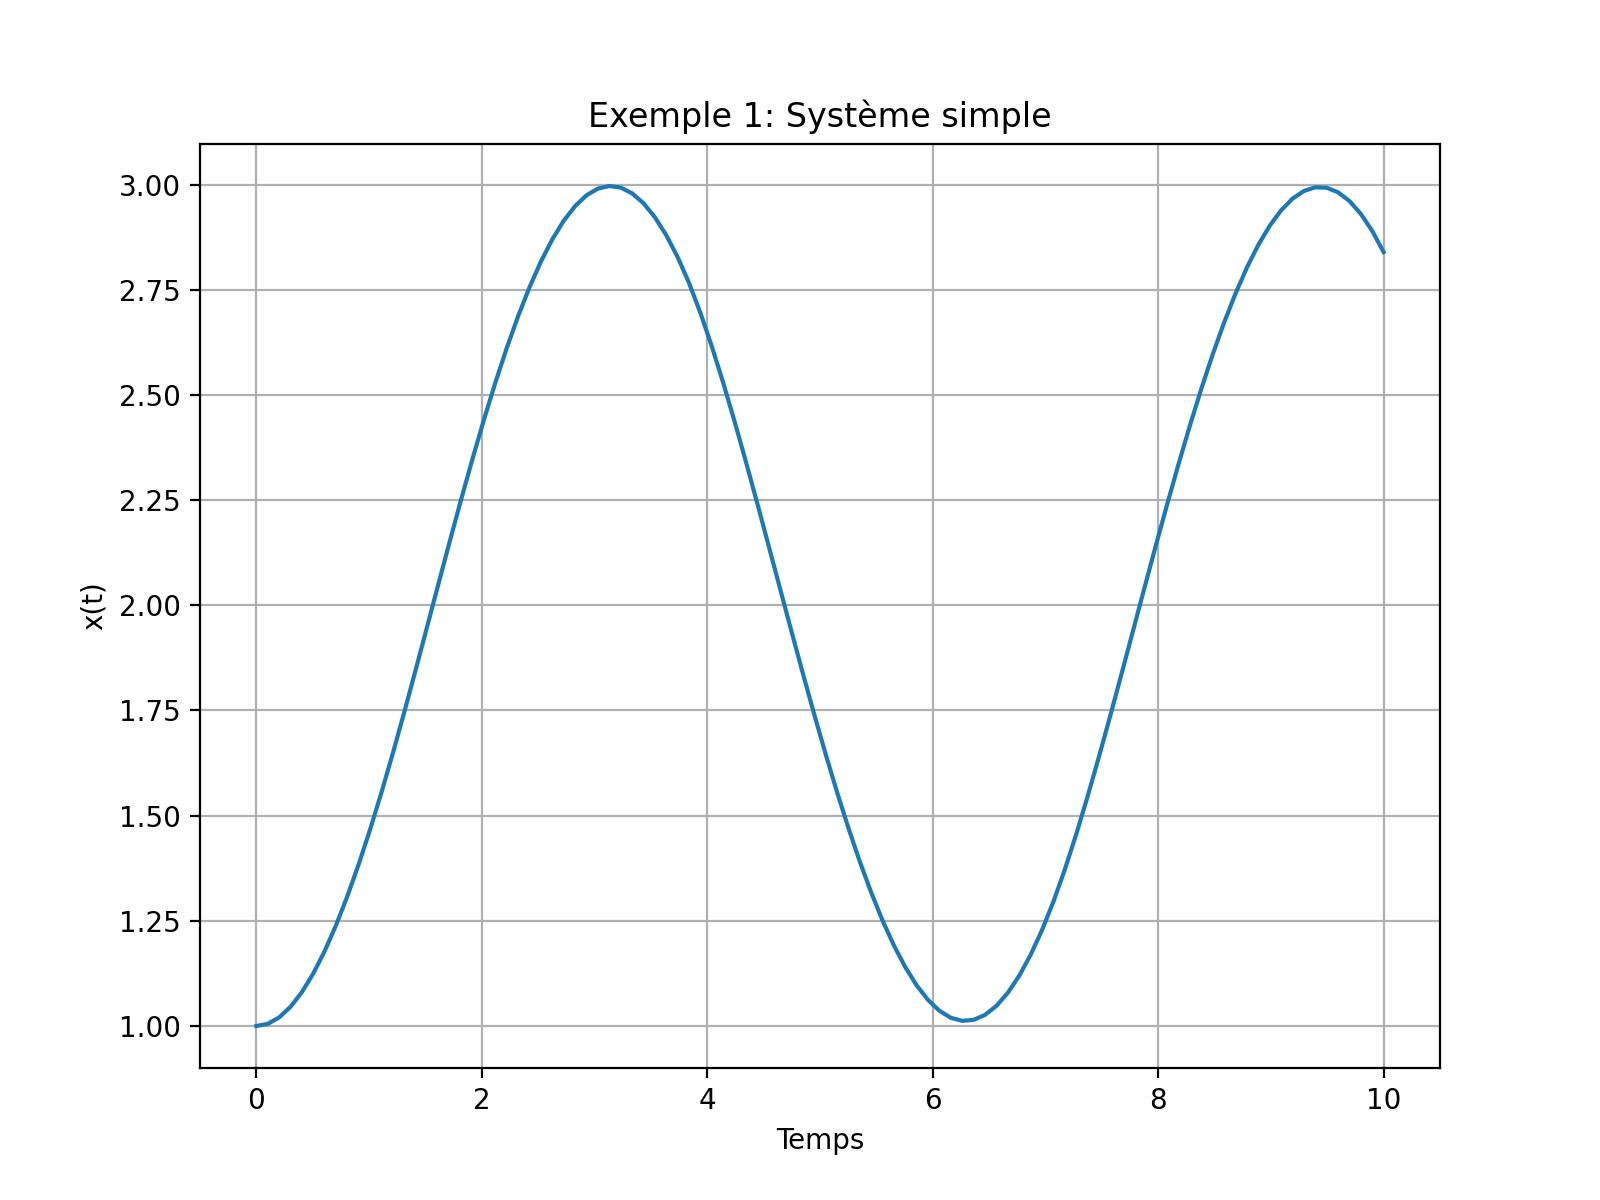
\includegraphics[width=\textwidth]{images/integrateur_simple.jpg}
                    \caption{Solution numérique de l'intégrateur simple}
                    \label{fig:integrateur_simple}
                \end{figure}

        \subsection{Croissance et décroissance exponentielle}
            Ce modèle a déjà été présenté dans le chapitre \ref{chap:equadiff}, dans lequel nous avons déterminé la solution analytique. Nous montrons que cette solution peut être aussi obtenue numériquement. Le système est décrit par
            \begin{equation*}
            \begin{cases}
            x'(t)=c\,x(t)\\
            y(t)=x(t)
            \end{cases}
            \end{equation*}
            avec les conditions suivantes :
            \begin{itemize}
                \item Condition initiale: $x(0)=1$,
                \item Valeur du paramètre: $c=0.1$,
                \item Intervalle temporel: $[0,10]$.
            \end{itemize}
        
            \subsubsection{Solution numérique}
                Ce code résout le système exponentiel et affiche le graphique de la solution en Figure \ref{fig:croissance_exponentielle}. \robin{Again, faire le lien avec la solution $x(t) = \exp(t/10)$~?}
                \inputminted{python}{codes/croissance_exponentielle.py}
                \begin{figure}[ht!]
                    \centering
                    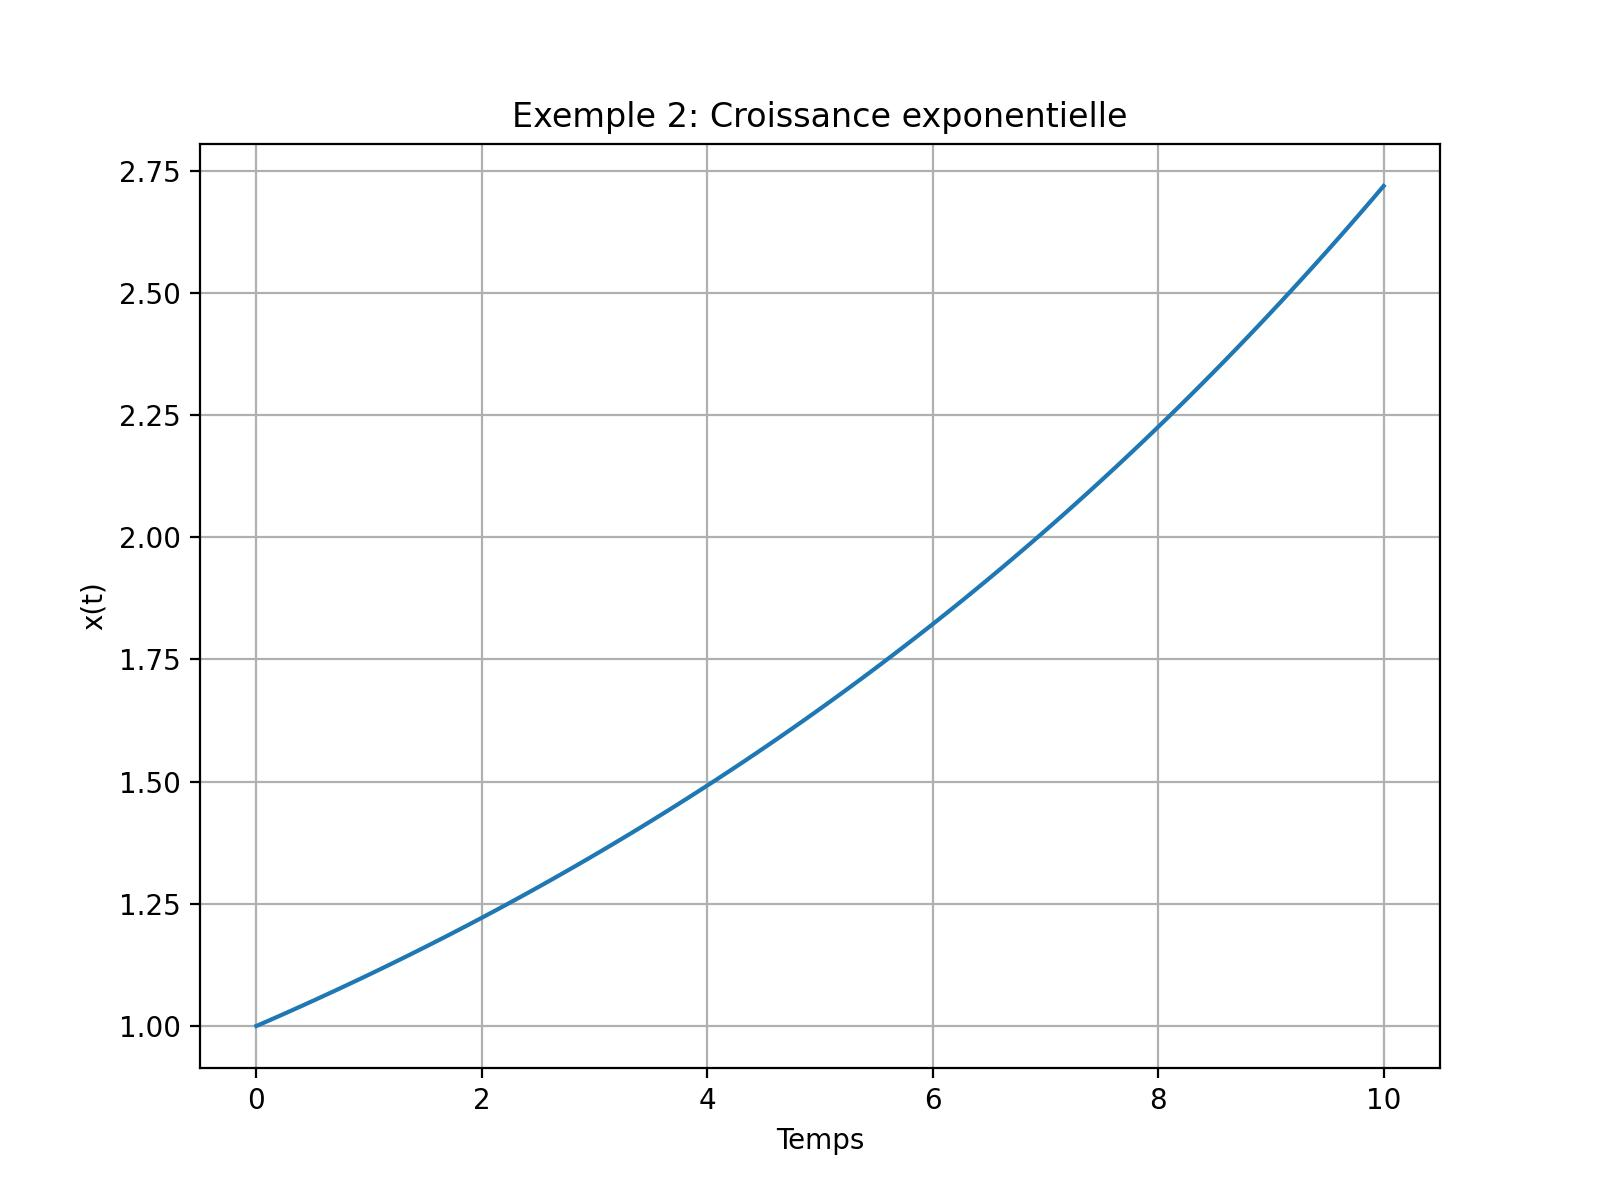
\includegraphics[width=\textwidth]{images/croissance_exponentielle.jpg}
                    \caption{Solution numérique de la croissance exponentielle}
                    \label{fig:croissance_exponentielle}
                \end{figure}

        \subsection{Système avec retard d'ordre 1}
            Pour illustrer les effets d'un retard dans un système dynamique, nous utilisons un modèle simple avec une entrée constante :
            \begin{equation*}
            \begin{cases}
            x'(t)=u(t)-cx(t)\\
            y(t)=x(t)
            \end{cases}
            \end{equation*}
            avec les paramètres:
            \begin{itemize}
                \item Condition initiale: $x(0)=1$,
                \item Paramètre: $c=2$,
                \item Intervalle temporel: $[0,10]$,
                \item Entrée: $u(t)=1$ pour $t>0$.
            \end{itemize}
        
            \subsubsection{Solution numérique}
                La solution numérique est obtenue avec le code suivant. Le graphique correspondant est présenté en Figure \ref{fig:retard}. \robin{Again, faire le lien avec la solution $x(t) = (1 + \exp(-2t)) / 2$~?}
                \inputminted{python}{codes/retard.py}
                \begin{figure}[ht!]
                    \centering
                    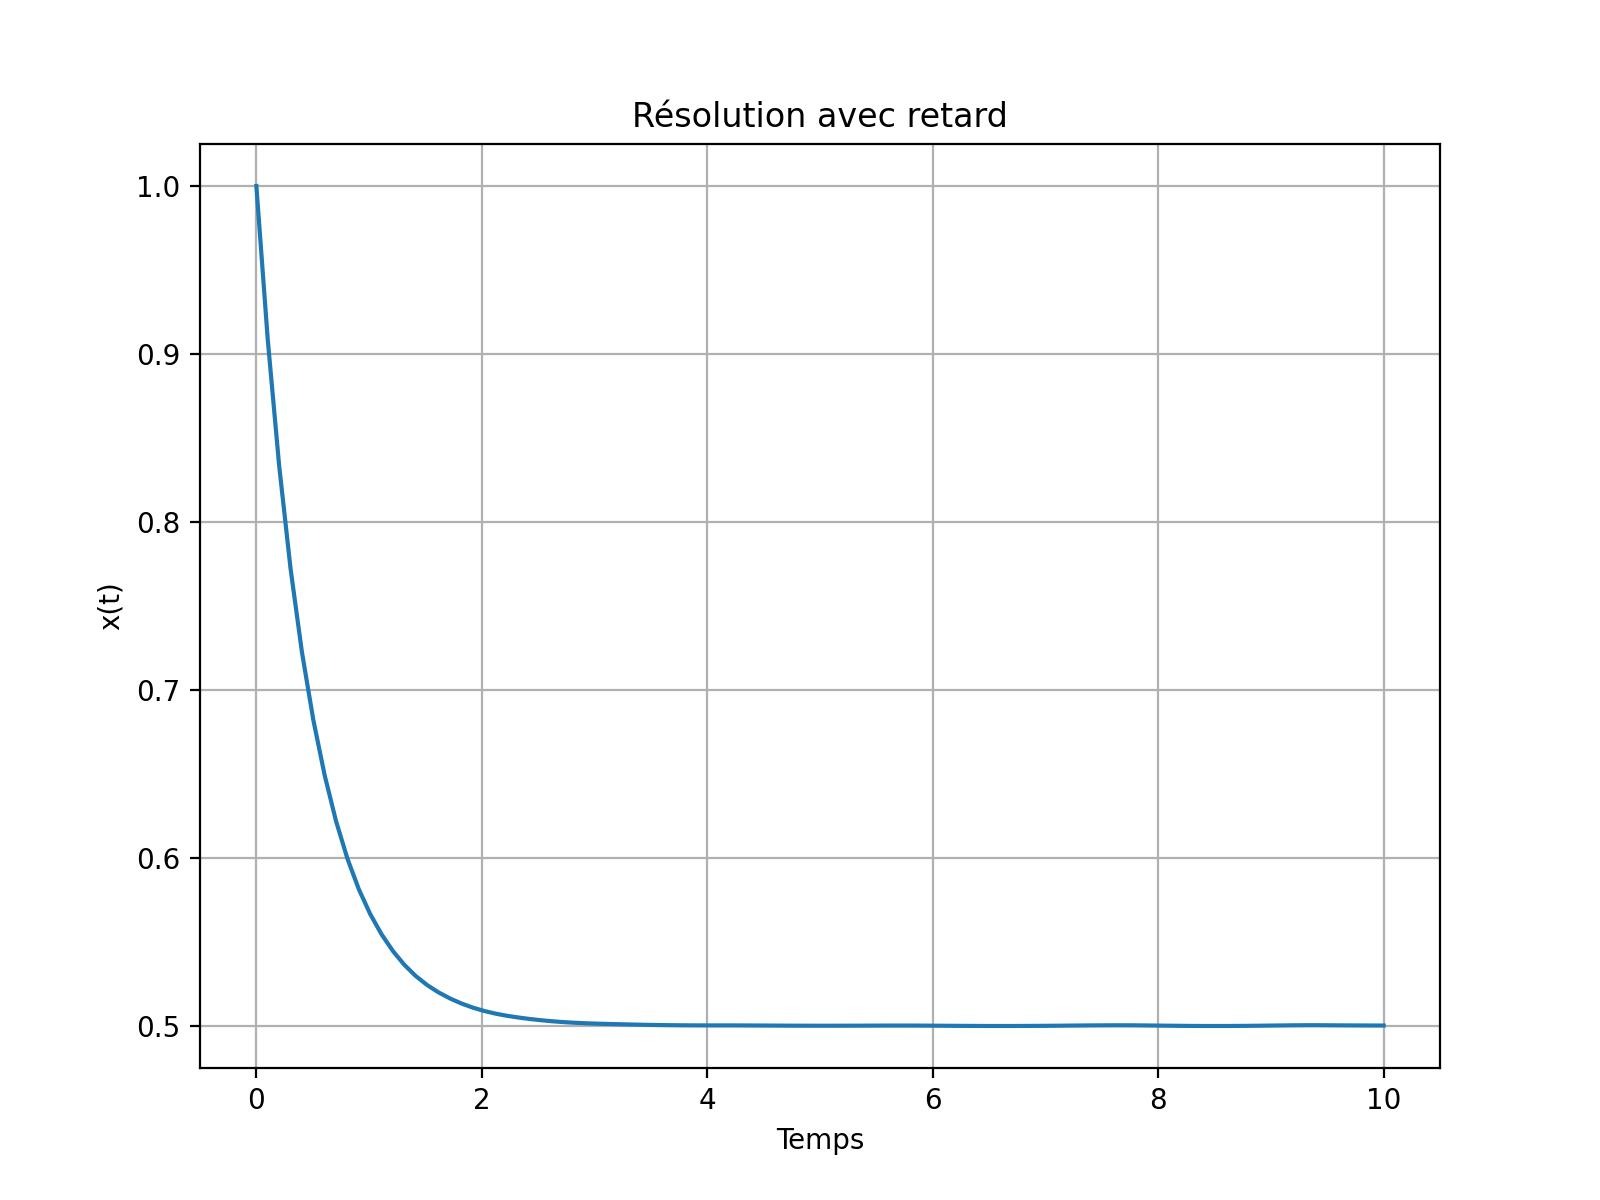
\includegraphics[width=\textwidth]{images/retard.jpg}
                    \caption{Solution numérique du système avec retard}
                    \label{fig:retard}
                \end{figure}

        \subsection{Croissance logistique}
            Le modèle logistique est largement utilisé pour représenter la croissance de populations soumises à une capacité limite \footnote{\url{https://fr.wikipedia.org/wiki/Fonction_logistique_(Verhulst)}}:
            \begin{equation*}
            \begin{cases}
            x'(t)=c\,x(t)\left(1-\frac{x(t)}{k}\right)\\
            y(t)=x(t)
            \end{cases}
            \end{equation*}
            Les conditions sont:
            \begin{itemize}
                \item Condition initiale: $x(0)=0.3$,
                \item Paramètres: $k=1.5$, $c=0.2$,
                \item Intervalle temporel: $[0,50]$.
            \end{itemize}
        
            \subsubsection{Solution numérique}
                Ce code montre la convergence vers la capacité limite du modèle logistique. Le graphique est présenté en Figure \ref{fig:logistique}.
                \inputminted{python}{codes/logistique.py}
                \begin{figure}[ht!]
                    \centering
                    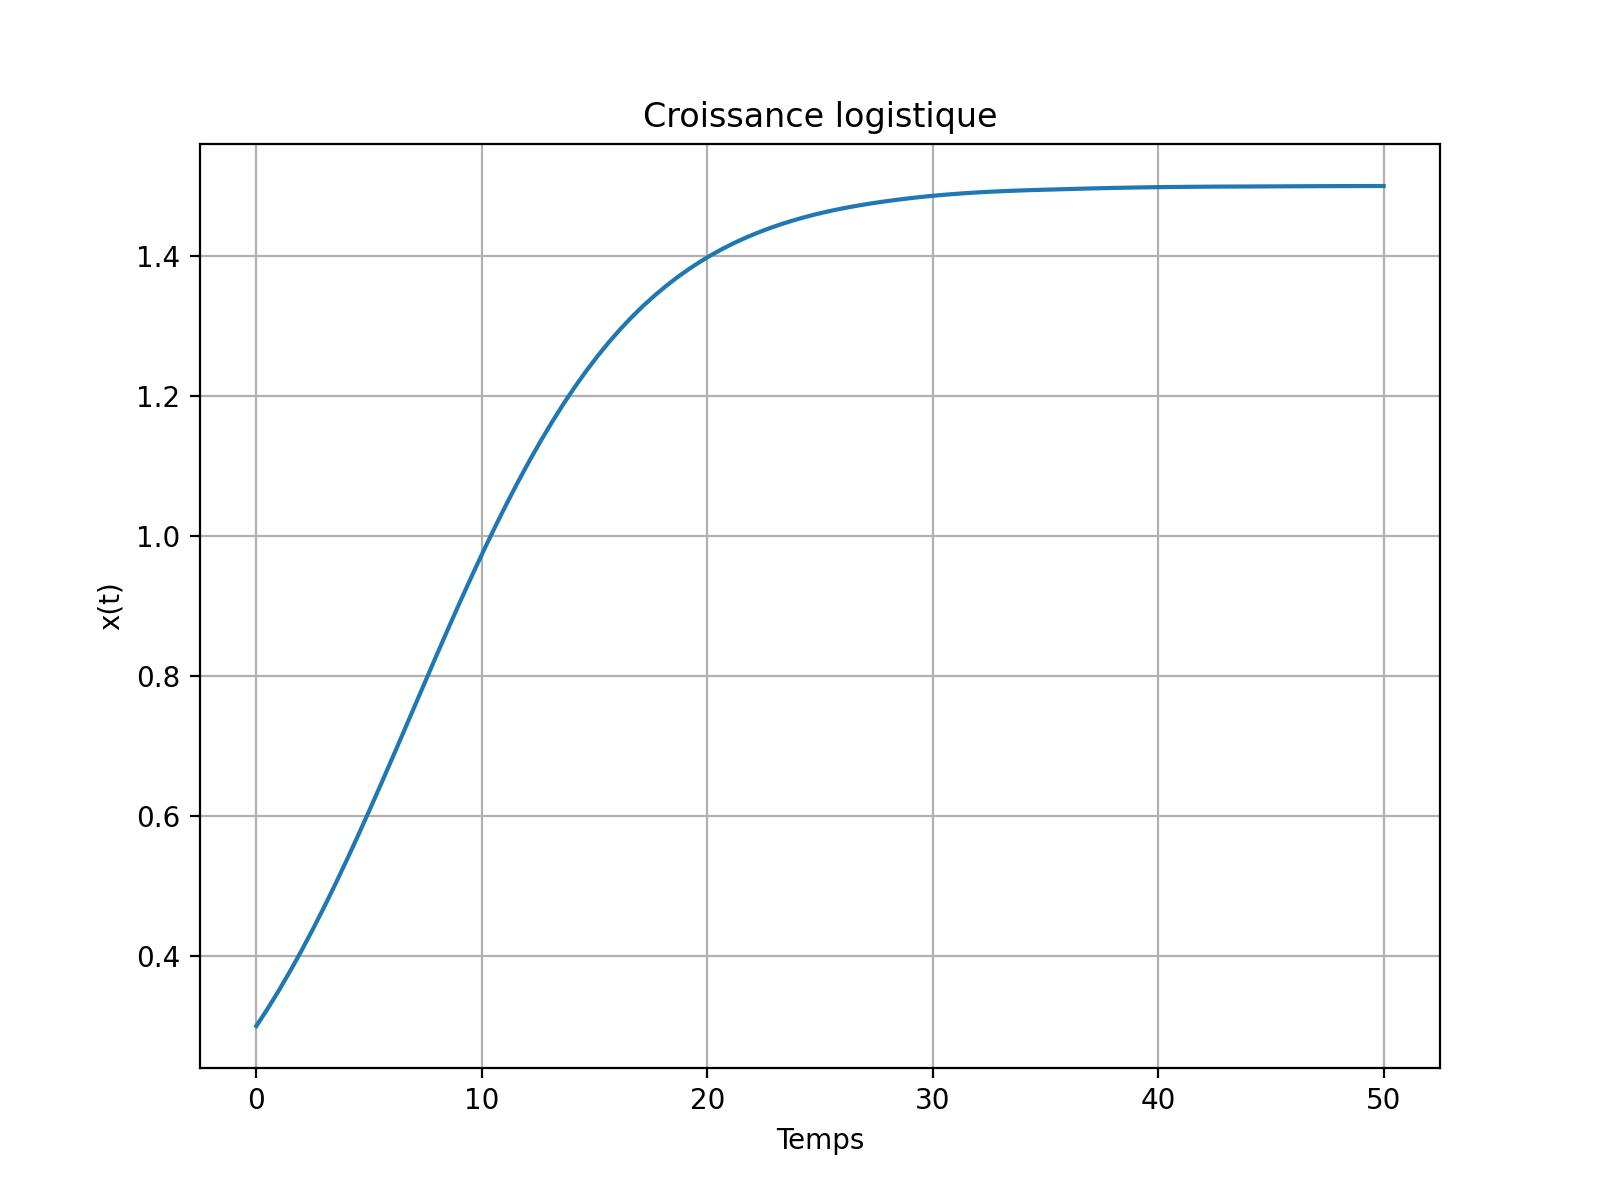
\includegraphics[width=\textwidth]{images/logistique.jpg}
                    \caption{Solution du modèle de croissance logistique}
                    \label{fig:logistique}
                \end{figure}
                
                En variant les conditions initiales, nous pouvons observer leur effet sur la dynamique de la population en Figure \ref{fig:logistique2}.
                \begin{figure}[ht!]
                    \centering
                    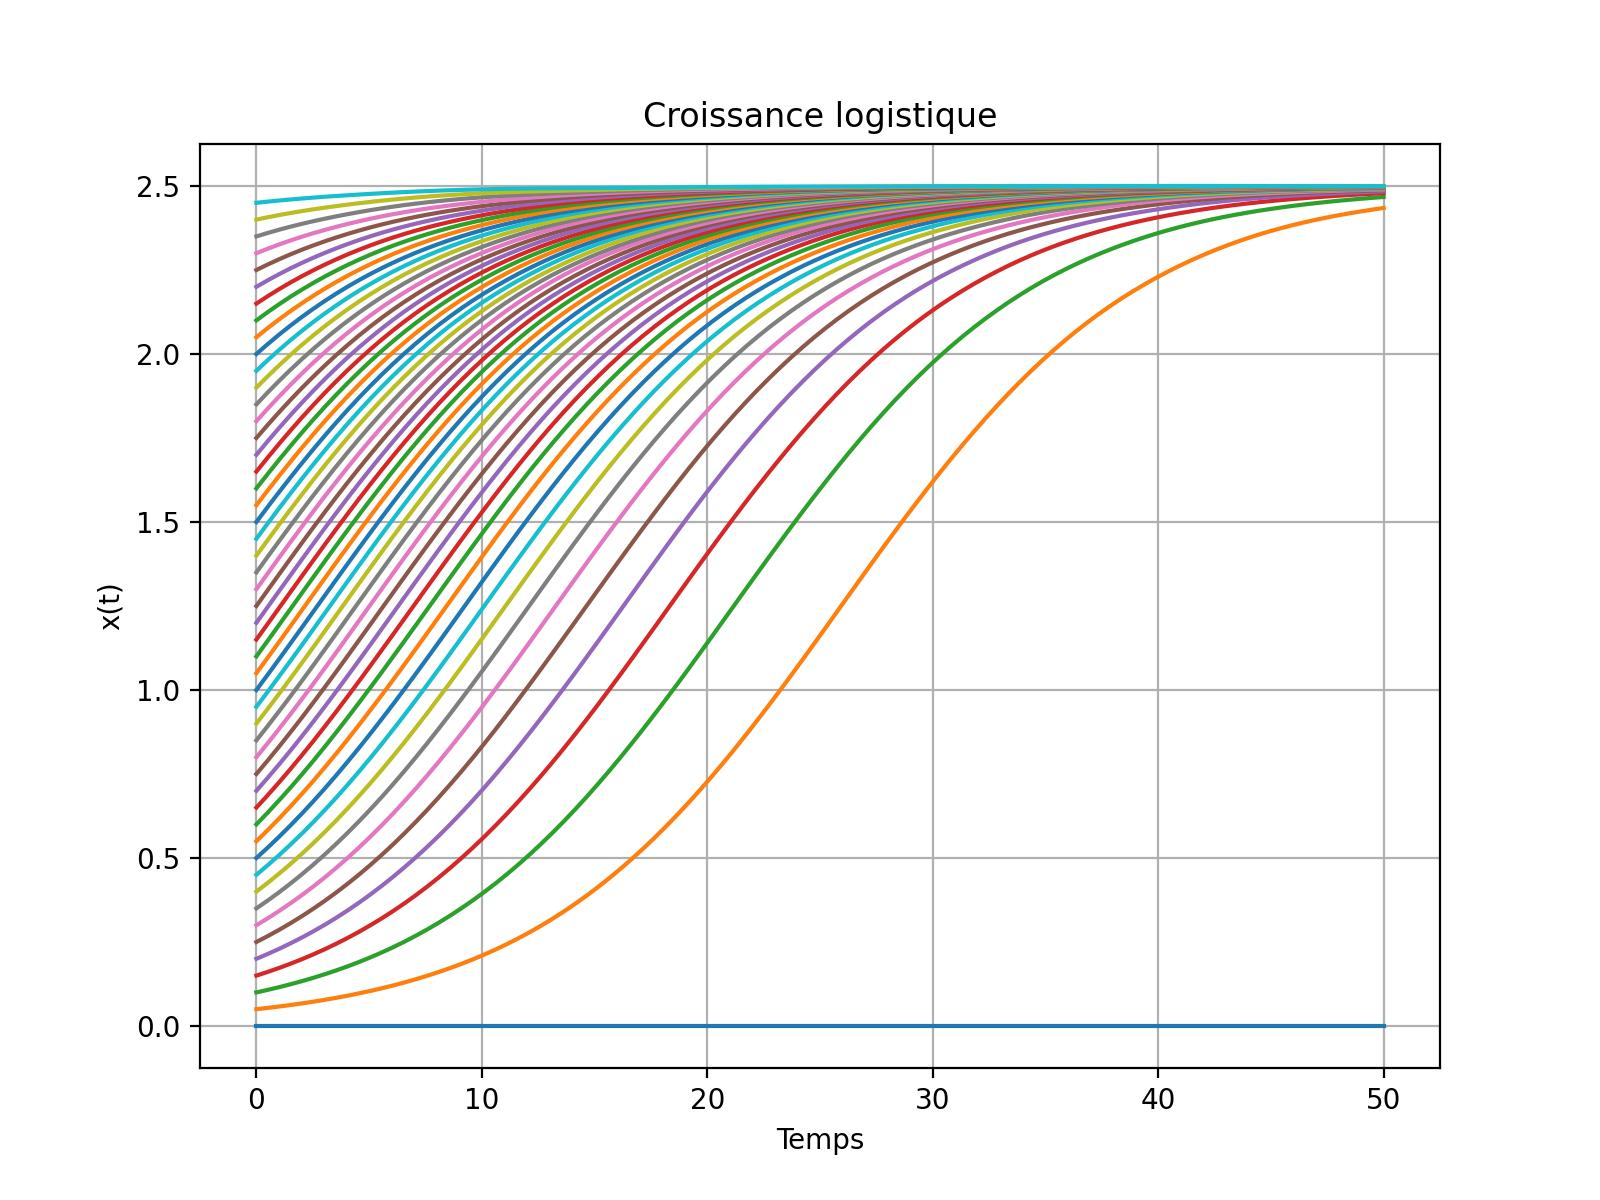
\includegraphics[width=\textwidth]{images/logistique2.jpg}
                    \caption{Effet des conditions initiales sur la croissance logistique}
                    \label{fig:logistique2}
                \end{figure}
    \section{Simulation de systèmes linéaires d'ordre 2}
        Les étapes pour la simulation et le dessin de portrait de phases des systèmes d'ordre deux sont les mêmes que celles vues dans le chapitre \ref{chap:portrait_phases}. Pour un système
        \begin{equation*}
            x'(t) = A x(t)
        \end{equation*}
        Les étapes à suivre sont les suivantes
        \begin{enumerate}
            \item Dessin des droites invariantes (vecteurs propres)~;
            \item Dessin des isoclines~;
            \item Dessin de vecteurs vitesse~;
            \item Dessin de trajectoire.
        \end{enumerate}
        \subsection{Exercices}
            \subsubsection{Trajectoire}
                \begin{exercise}{Trajectoire}
                    Écrivez une fonction \codeword{trajectoire(A: list[list], interval: list[int], c_i: list[int])->None} qui prend en paramètre une matrice \codeword{A}, un intervalle de simulation et une condition initiale, et qui affiche la trajectoire dans le portrait de phase. Utilisez \codeword{Numpy}, \codeword{SciPy} et \codeword{matplotlib}.
                \end{exercise}
                La solution est donnée par le code suivant, dont le résultat pour la matrice
                \begin{equation*}
                    A = \begin{bmatrix}-2 & 1\\ 1 & -2\end{bmatrix}
                \end{equation*}
                est donné dans la figure \ref{fig:trajectoire}
                \inputminted{python}{codes/trajectoire.py}
                \begin{figure}[ht!]
                    \centering
                    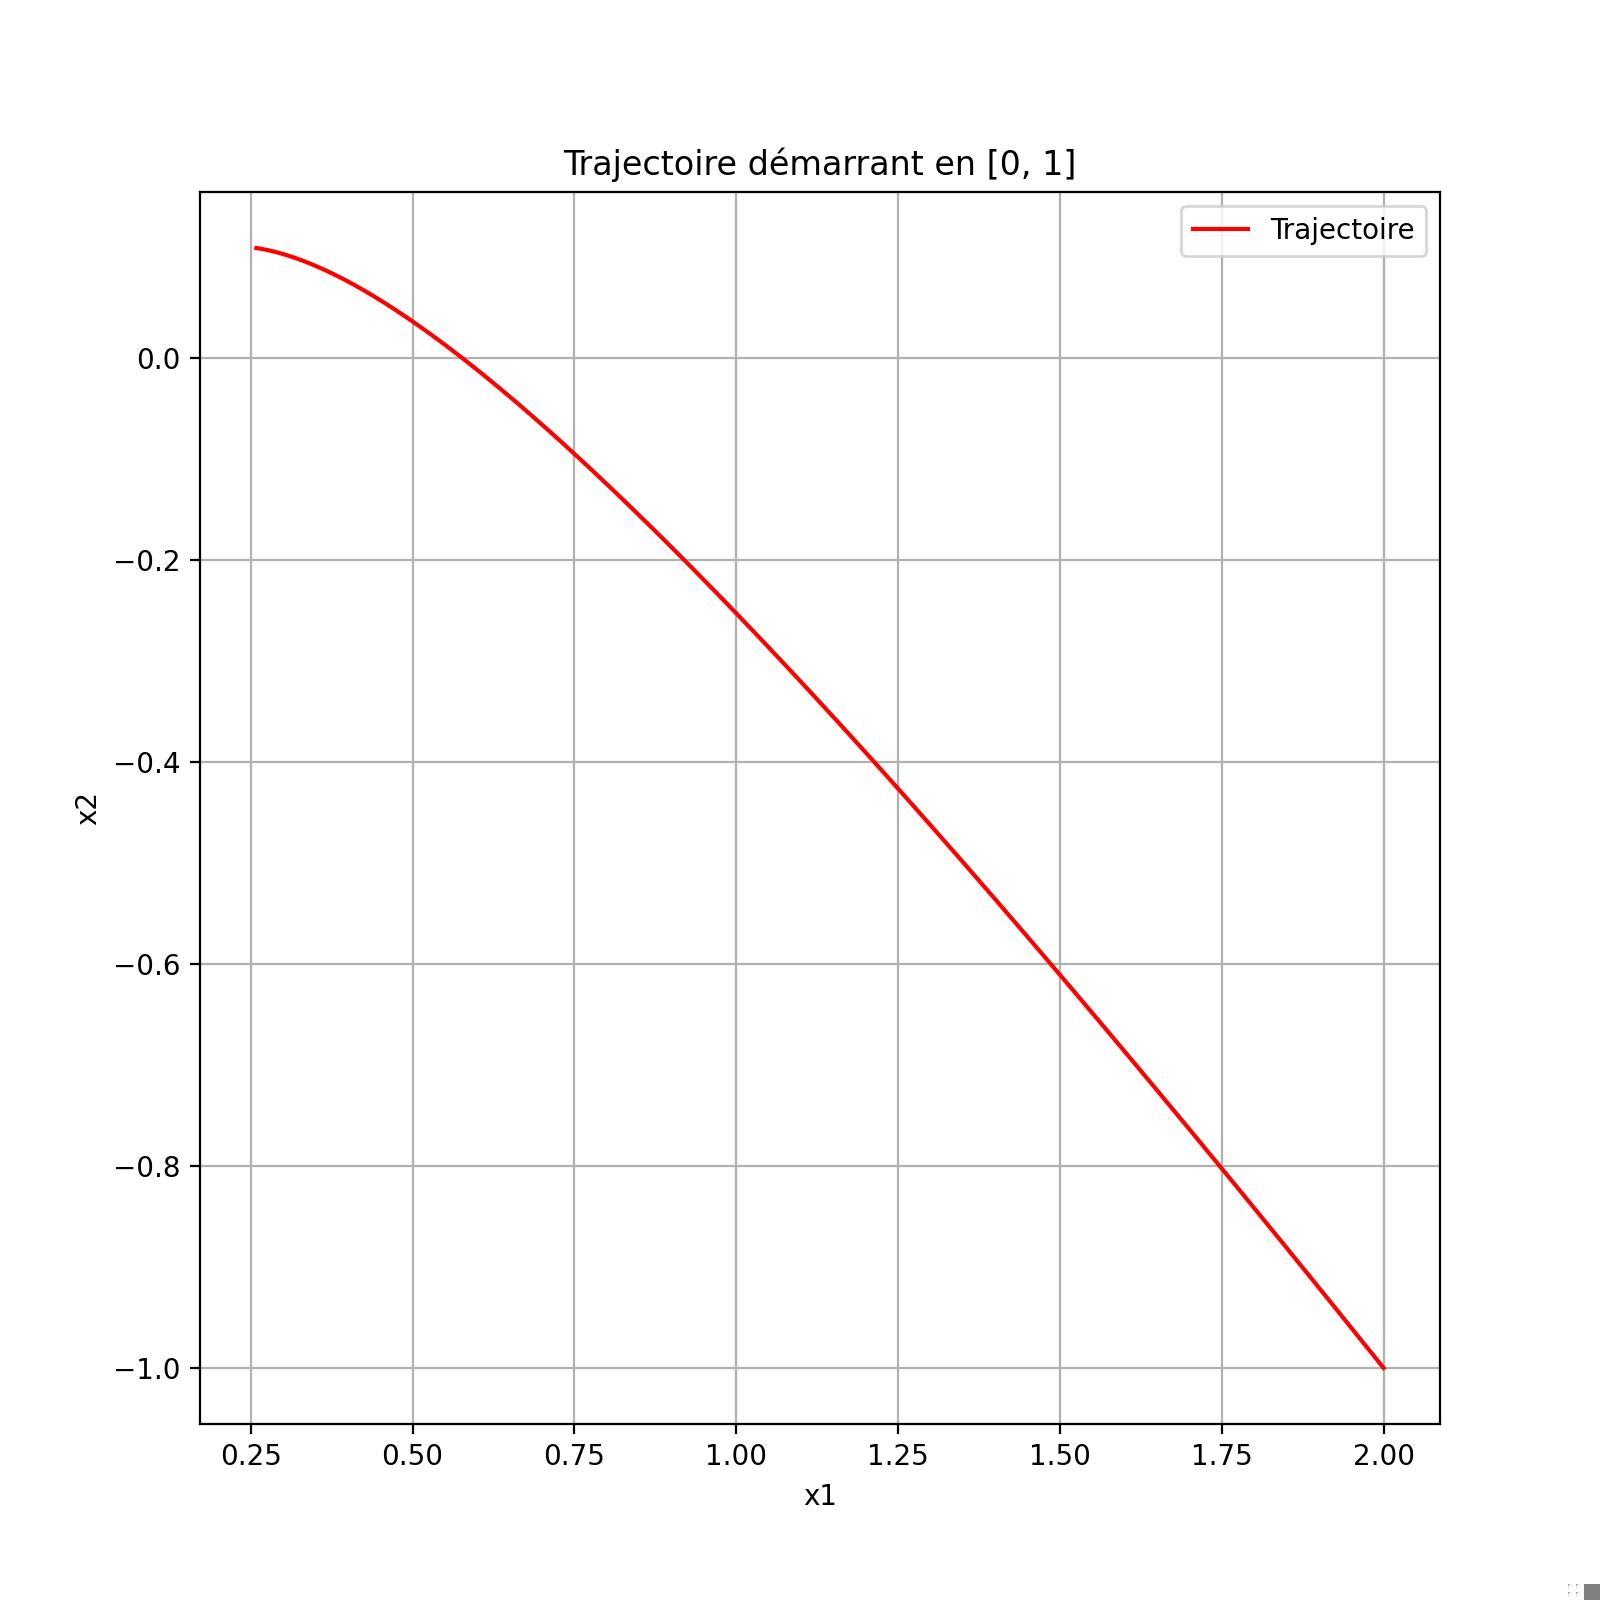
\includegraphics[width=\textwidth]{images/trajectoire.jpg}
                    \caption{Exemple de trajectoire}
                    \label{fig:trajectoire}
                \end{figure}
                
            \subsubsection{Vecteurs propres et droites invariantes}
                On veut dessiner plusieurs choses sur la même figure:
                \begin{itemize}
                    \item deux droites pour les vecteur propres~;
                    \item les flèches des vecteurs propres.
                \end{itemize}
                Pour dessiner les droites des vecteurs propres, il faut calculer la pente de la droite.
                Les vecteurs propres peuvent être calculés en utilisant la fonction \codeword{eig} du module \codeword{linalg} (pour \textit{linear algebra}) de \codeword{Numpy}.
                Les composantes de ces vecteurs propres peuvent être utilisés pour trouver la pente de la droite associée.

                \begin{exercise}{Vecteurs propres et droites invariantes}
                    Écrivez une fonction \codeword{vecteurs_propres(A: list[list])->None} qui prend en paramètre une matrice A et qui dessine les vecteurs propres et leurs droites associées.
                \end{exercise}
                
                La solution est donnée par le code suivant, dont le résultat pour la même matrice est donné dans la figure \ref{fig:invariants}
                \inputminted{python}{codes/invariants.py}
                \begin{figure}[ht!]
                    \centering
                    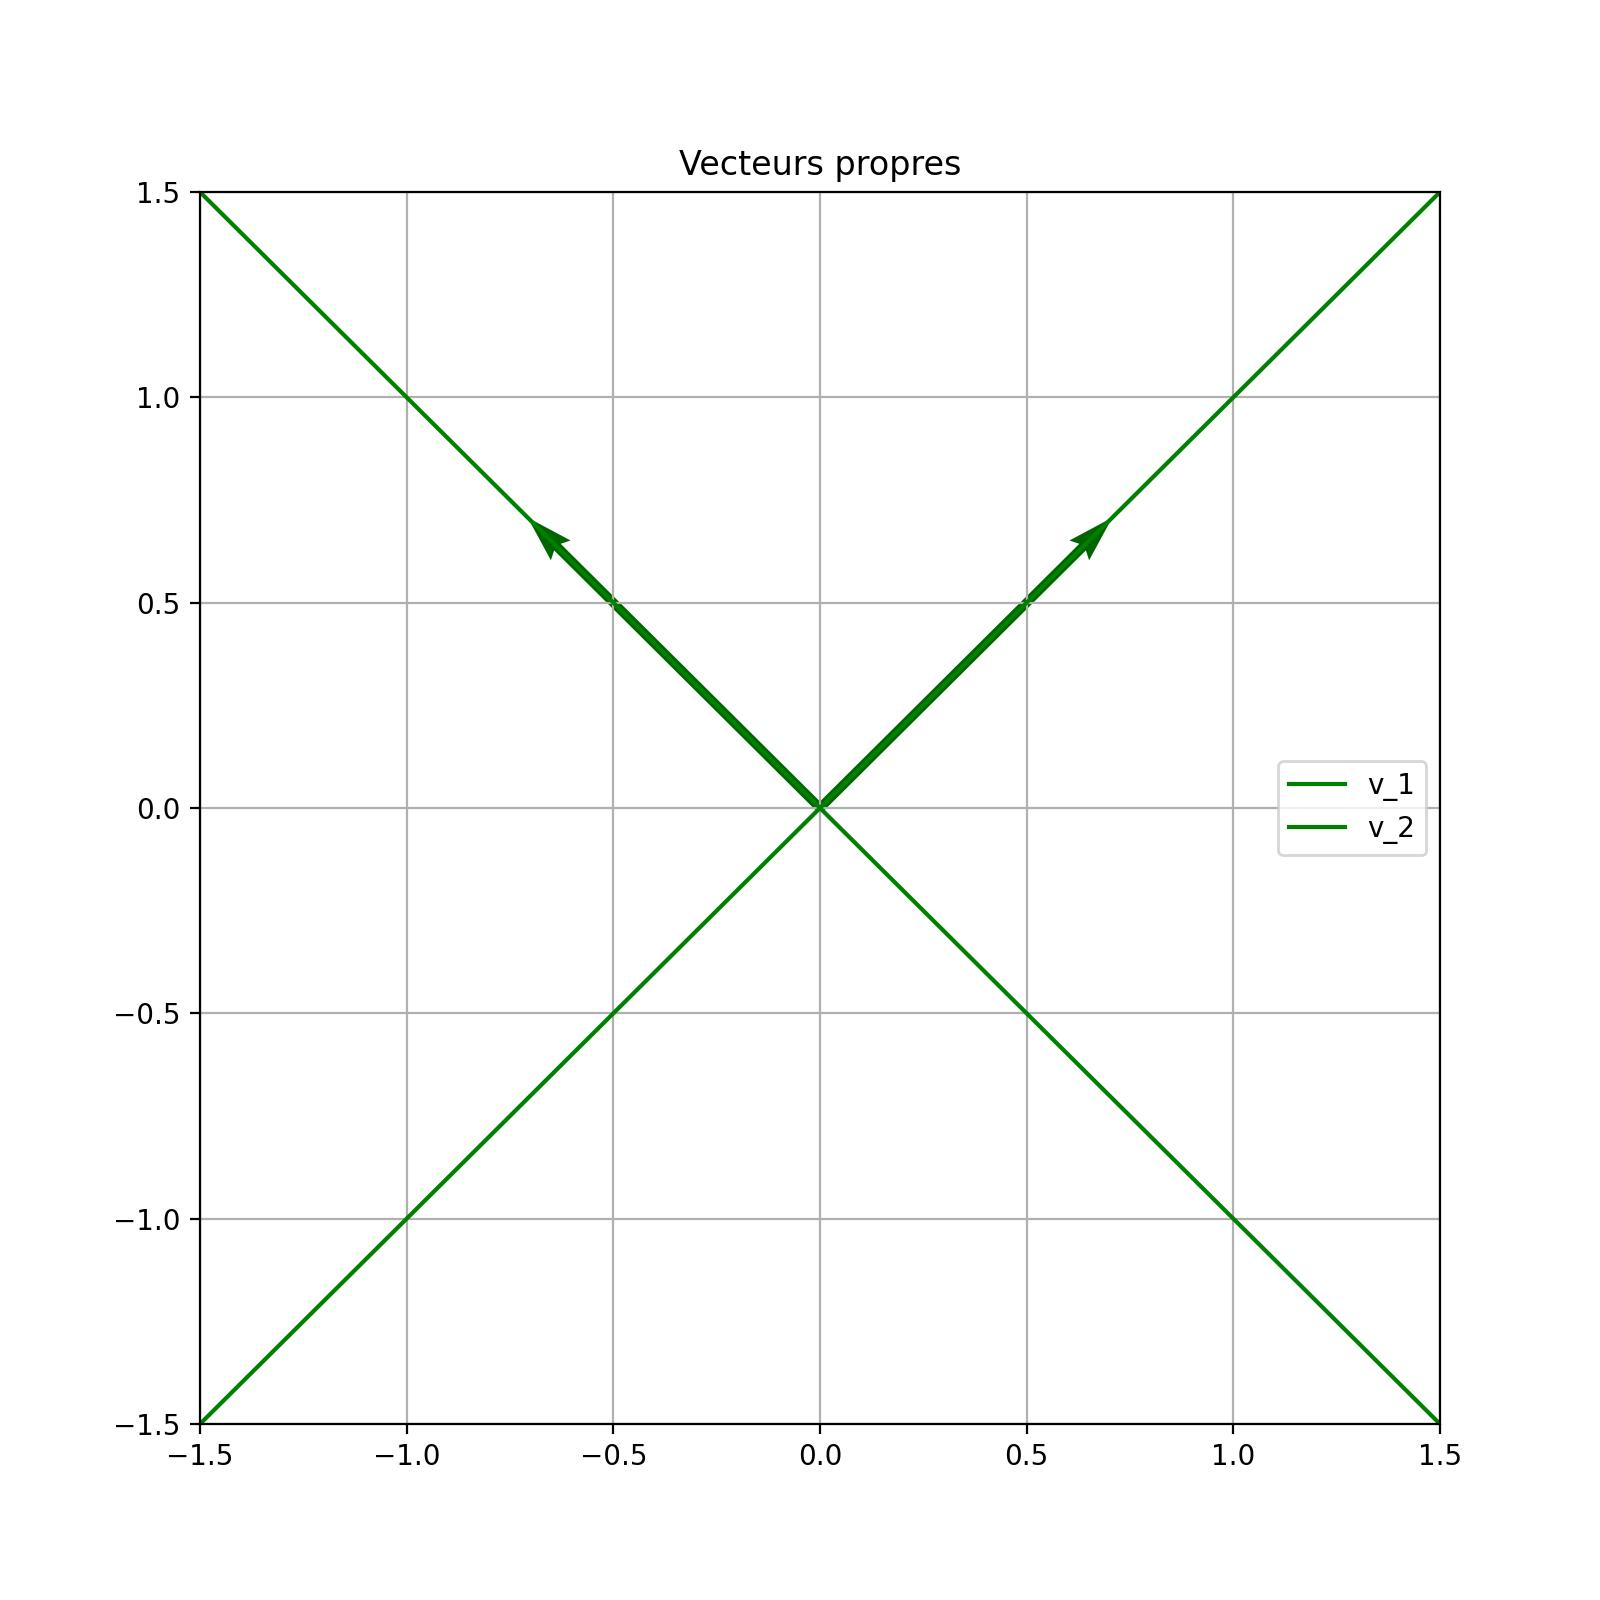
\includegraphics[width=\textwidth]{images/invariants.jpg}
                    \caption{Exemple de vecteurs propres et de droites invariantes}
                    \label{fig:invariants}
                \end{figure}

            \subsubsection{Isoclines}
                Le calcul des isoclines peut se faire d'une manière comparable aux vecteurs propres en exprimant $x_2$ en fonction de $x_1$.
                Comme
                \begin{equation*}
                    \begin{cases}
                        \dot{x_1} = a_{11}x_1 + a_{12} x_2\\
                        \dot{x_2} = a_{21}x_1 + a_{22} x_2
                    \end{cases}
                \end{equation*}
                
                Et que les isoclines sont la solution à \robin{Attention~: avec les accolades, on dirait que tu essayes de résoudre le système. Or si $A$ est inversible, la seule solution serait $x = [0, 0]^\top$ (qui est le seul ponit simultanément dans les deux isoclines)}~:
                
                \begin{equation*}
                    \begin{cases}
                        0 = a_{11}x_1 + a_{12} x_2\\
                        0 = a_{21}x_1 + a_{22} x_2
                    \end{cases}
                    \Longleftrightarrow
                    \begin{cases}
                        a_{12} x_2 = -a_{11}x_1\\
                        a_{22} x_2 = -a_{21}x_1
                    \end{cases}
                    \Longleftrightarrow
                    \begin{cases}
                        x_2 = -\frac{a_{11}}{a_{12}}x_1\\
                        x_2 = -\frac{a_{21}}{a_{22}}x_1
                    \end{cases}
                \end{equation*}
                Ce qui nous donne une pente de $-\frac{a_{11}}{a_{12}}$ et $-\frac{a_{21}}{a_{22}}$ respectivement.

                \begin{exercise}{Isoclines}
                    Écrivez une fonction \codeword{isoclines(A: list[list])->None} qui prend en paramètre une matrice A et qui dessine les isoclines associées.
                \end{exercise}
                
                La solution est donnée par le code suivant, dont le résultat est donné dans la figure \ref{fig:isoclines2}.
                \inputminted{python}{codes/isoclines.py}
                \begin{figure}[ht!]
                    \centering
                    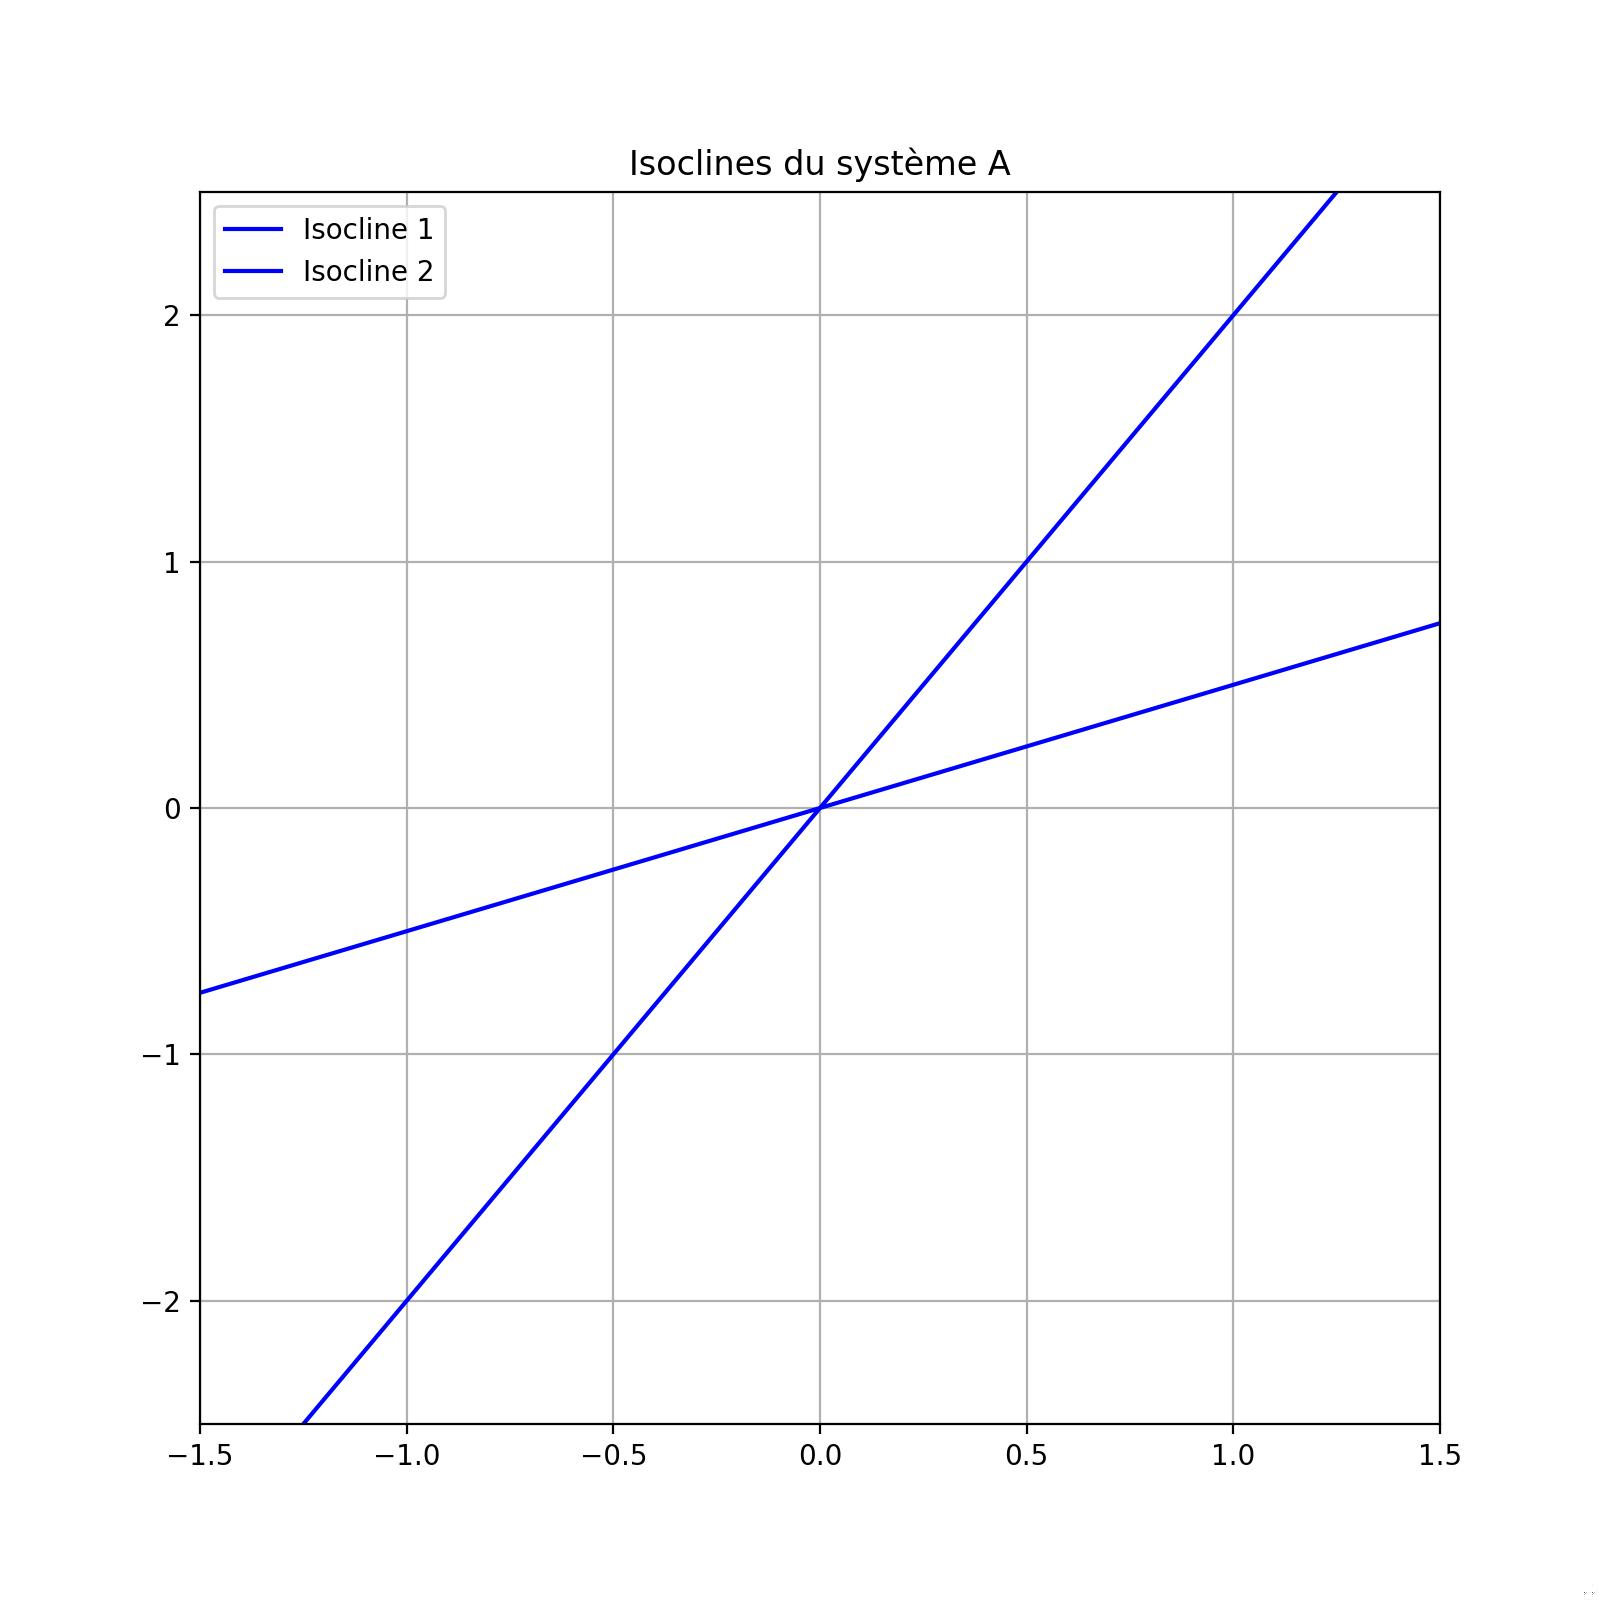
\includegraphics[width=\textwidth]{images/isoclines2.jpg}
                    \caption{Exemple d'isoclines}
                    \label{fig:isoclines2}
                \end{figure}
                
            \subsubsection{Champ de vecteurs vitesse}
                \begin{exercise}{Champ de vecteurs vitesse}
                    Écrivez une fonction \codeword{vecteurs_vitesse(A: list[list])->None} qui prend en paramètre une matrice A et un intervalle, et qui affiche le portrait de phase, pour tous les points situés sur une grille de taille de case $0.2$.
                \end{exercise}

                La solution est donnée par le code suivant, dont le résultat est donné dans la figure \ref{fig:champ_vecteurs_vitesse}.
                \inputminted{python}{codes/champ_vecteurs_vitesse.py}
                \begin{figure}[ht!]
                    \centering
                    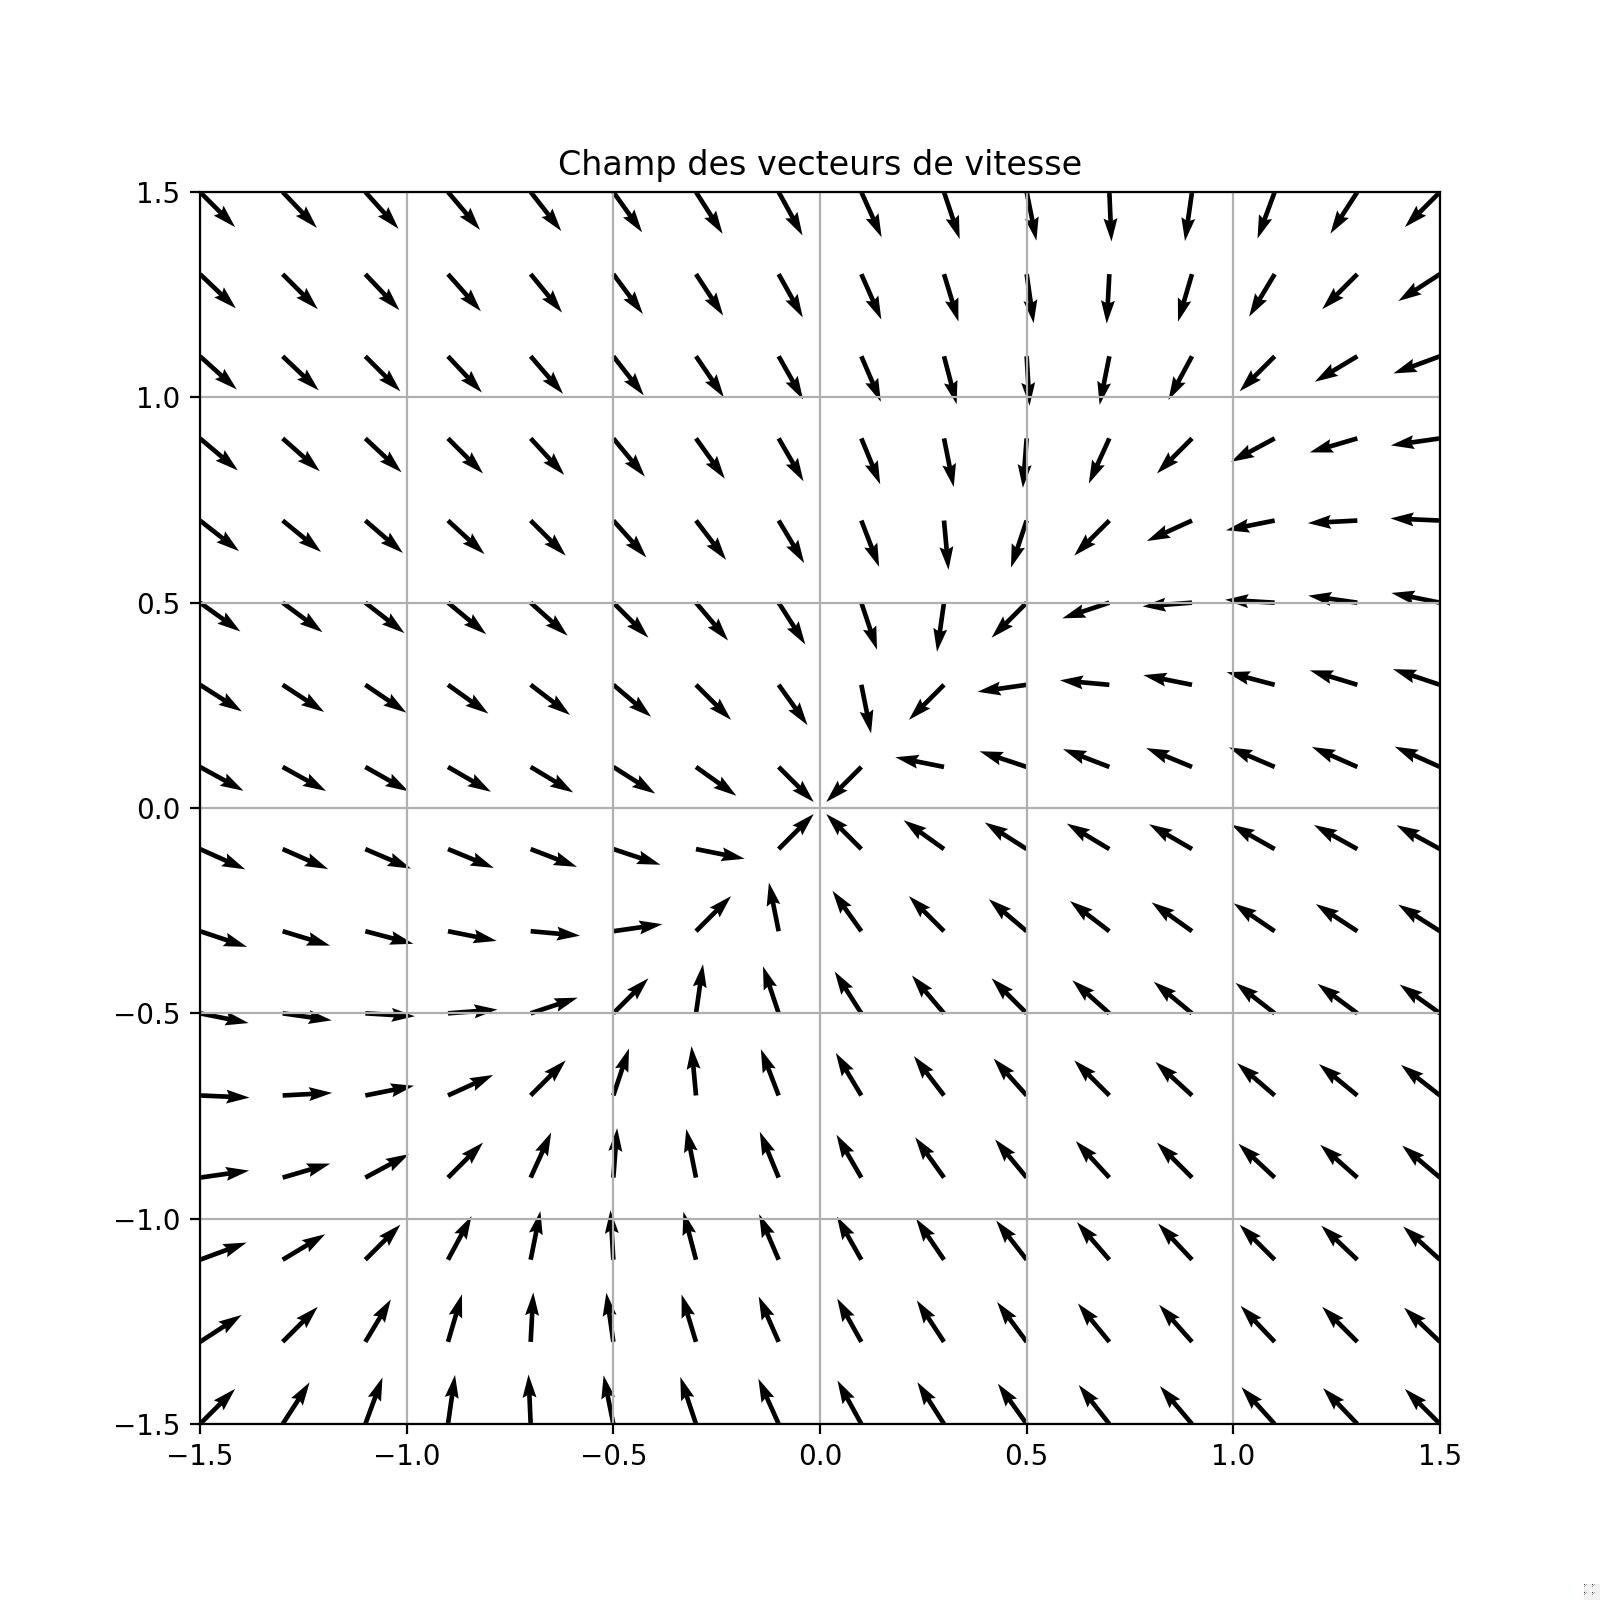
\includegraphics[width=\textwidth]{images/champ_vecteurs_vitesse.jpg}
                    \caption{Exemple de champ de vecteurs vitesse}
                    \label{fig:champ_vecteurs_vitesse}
                \end{figure}
                
            \subsubsection{Portrait de phases complet}
                \begin{exercise}{Portrait de phases}
                    Écrivez une fonction qui assemble tout le portrait de phase~:
                    \begin{itemize}
                        \item le champ de vecteurs~;
                        \item quatre trajectoires choisies arbitrairement~;
                        \item les isoclines~;
                        \item les vecteurs propres et les droites invariantes.
                        %\item 
                    \end{itemize}
                \end{exercise}

                La solution finale est donnée par le code suivant, dont le résultat est donné dans la figure \ref{fig:portrait_de_phases}.
                \inputminted{python}{codes/portrait_de_phases.py}
                \begin{figure}[ht!]
                    \centering
                    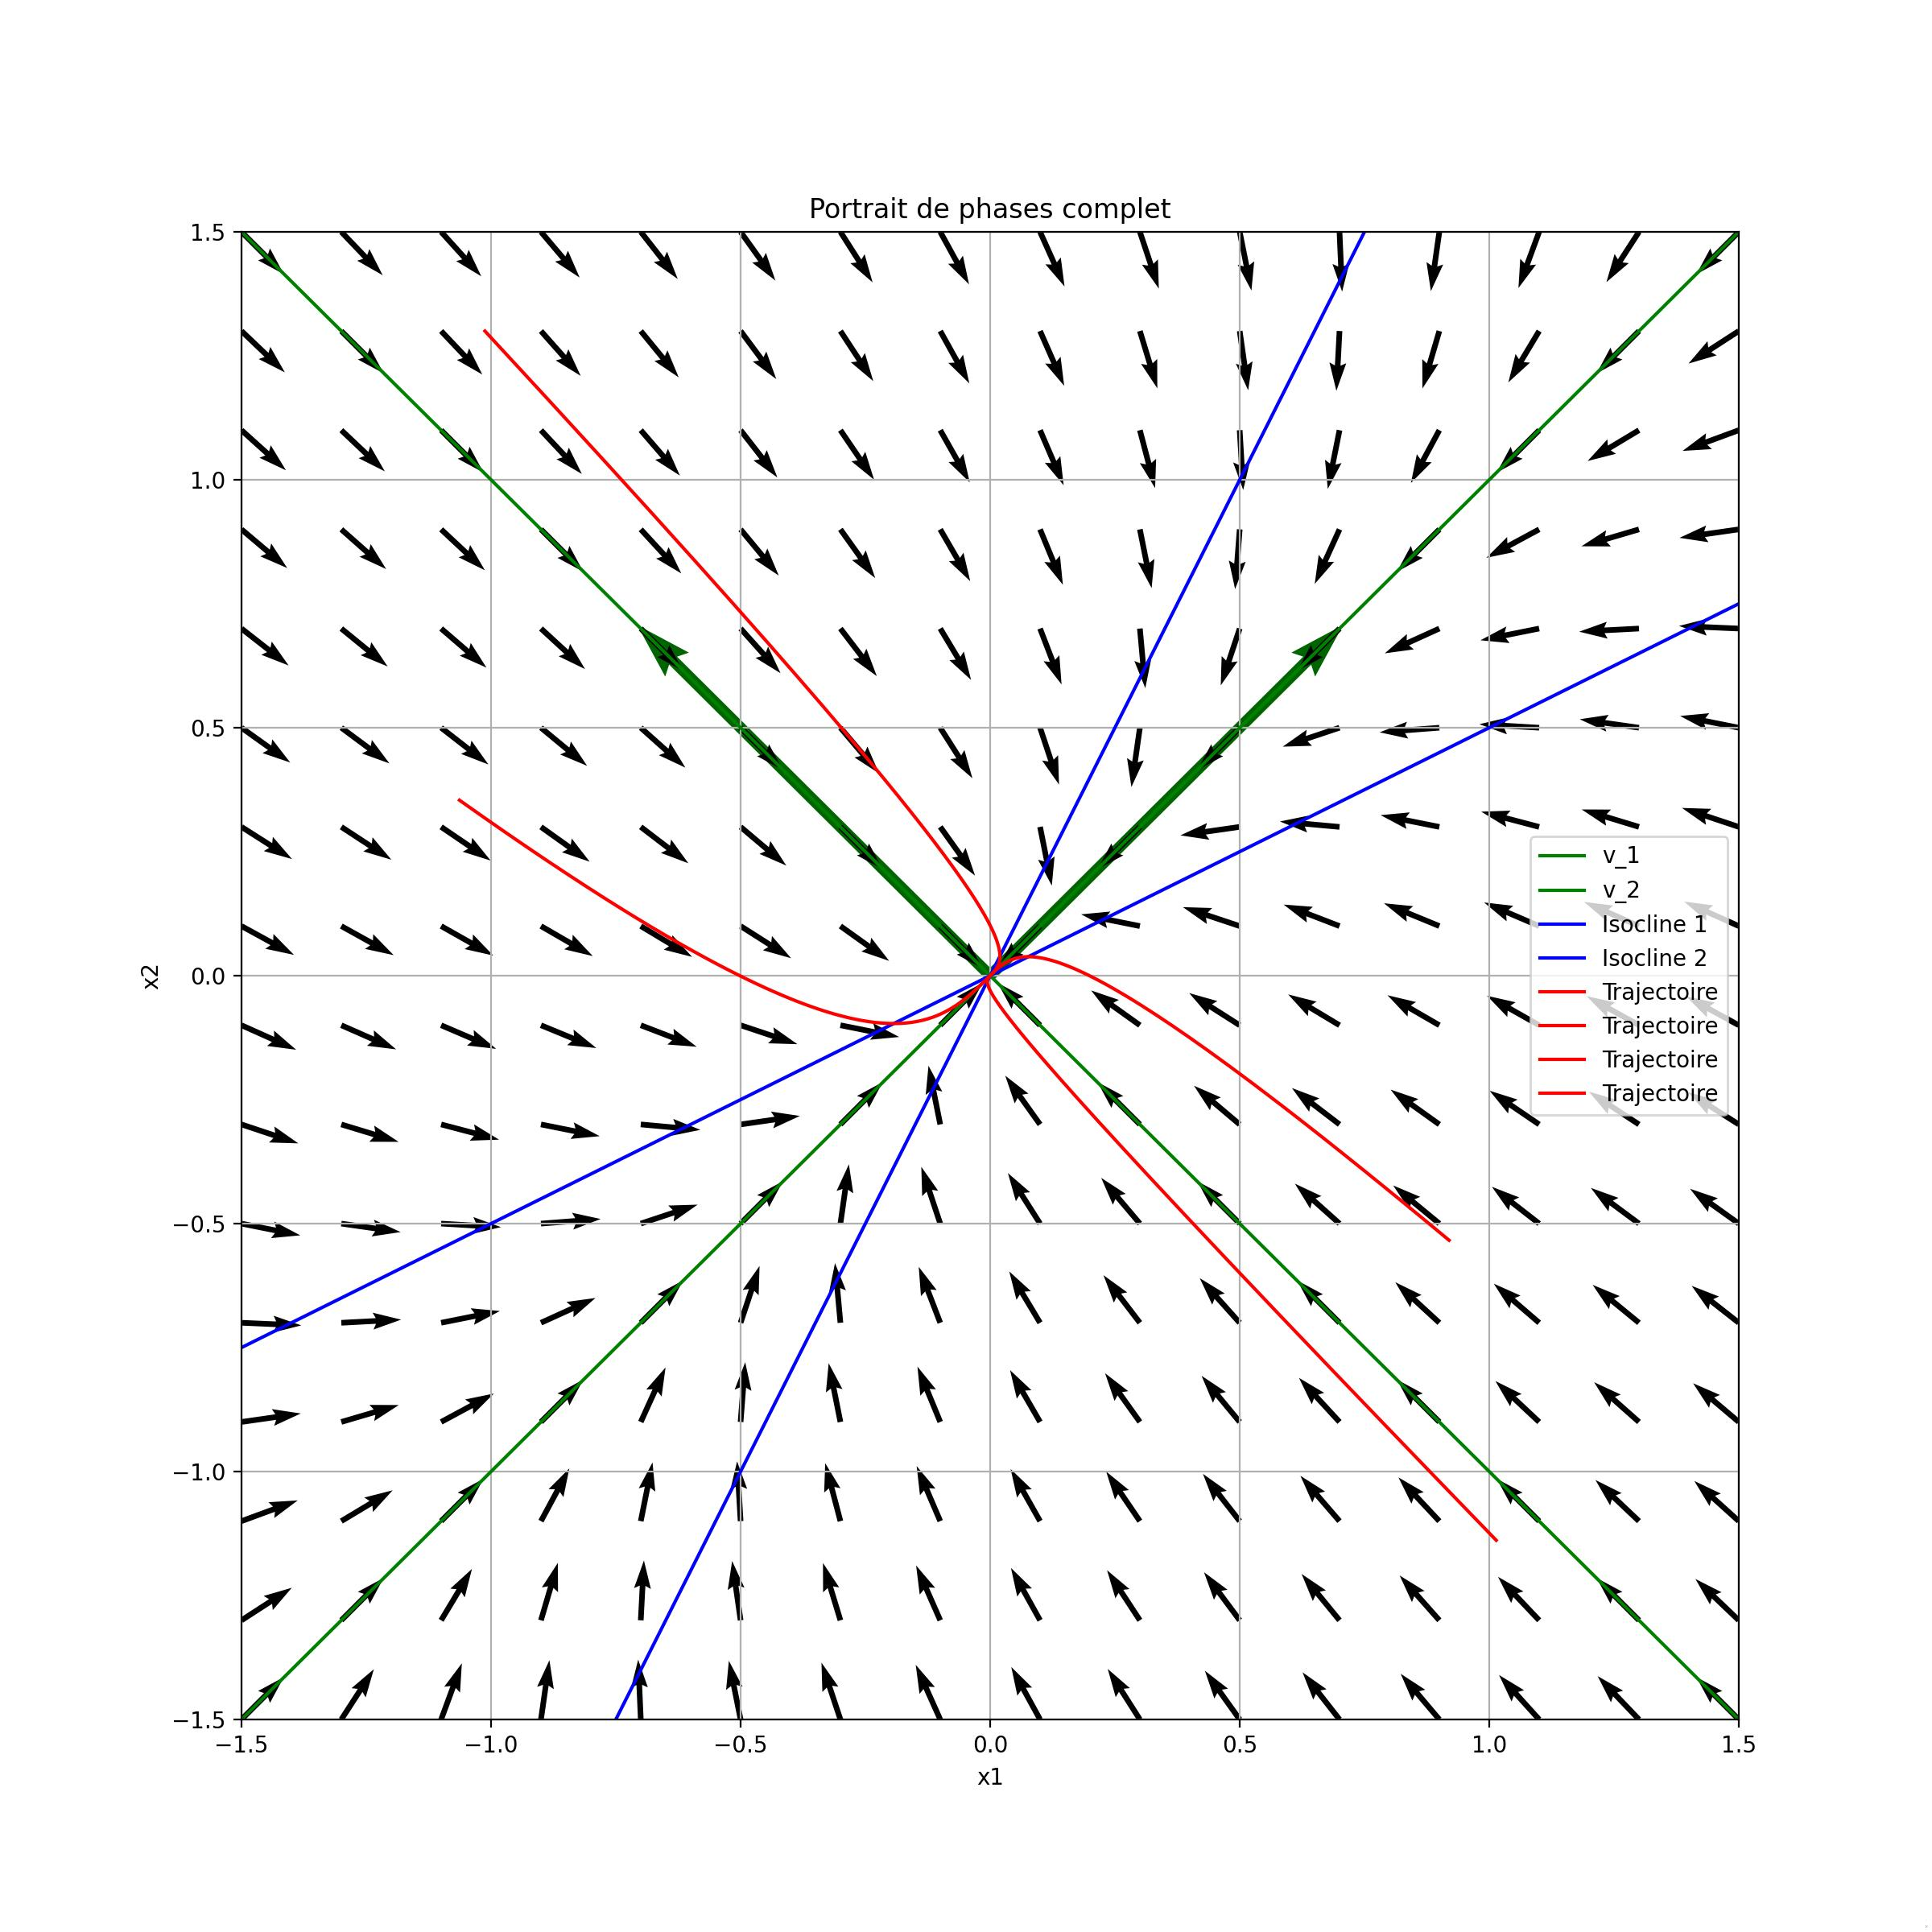
\includegraphics[width=\textwidth]{images/portrait_de_phases.jpg}
                    \caption{Exemple de portrait de phases}
                    \label{fig:portrait_de_phases}
                \end{figure}
    \section{Pour aller plus loin}
        Maintenant que le dessin de portrait de phases pour des systèmes linéaires d'ordre 2 a été extensivement abordé, il reste évidemment à aborder les systèmes non-linéaires. En pratique, la méthode reste la même que pour les systèmes linéaires, car la méthode de solution numérique s'applique aussi aux systèmes non-linéaires. Évidemment, certains raccourcis de calculs utilisés dans ce chapitre ne fonctionneront plus \textit{tels quels}: par exemple, le dessin d'une isocline ne sera vraisemblablement pas une droite. Certaines autres fonctions, comme celle du champ des vecteurs vitesses, peuvent être utilisées quelle que soit la (non-)linéarité du système, pour autant qu'il soit d'ordre 2.

        Pour les systèmes qui dépassent l'ordre 2, le défi technique devient alors la visualisation: le choix dépendra alors de l'application. Il vaudra mieux, parfois, afficher les trajectoires selon un sous-ensemble de paires de variables, ou préférer les animations. Ceci dépasse cependant le cadre de ce syllabus.
\chapter{Équations aux différences}
    \section{Introduction}
        Les équations aux différences sont au cœur de la modélisation de nombreux phénomènes dynamiques, lorsque leur formulation s'exprime en temps discret.

        L’étude des équations aux différences trouve ses racines dans les travaux des mathématiciens du XVIIe siècle, comme Pierre de Fermat et Blaise Pascal, qui utilisaient des suites arithmétiques et géométriques pour comprendre des phénomènes de croissance. Par exemple, les fameux nombres de Fibonacci, introduits en Occident par Leonardo Fibonacci au XIIIe siècle pour modéliser la croissance d’une population de lapins, sont représentés par une équation aux différences simple, mais élégante.

        Ce chapitre vise à fournir les outils nécessaires pour comprendre, formuler et résoudre des équations aux différences, en particulier celles de premier ordre et celles linéaires d'ordre supérieur. Nous allons aborder les notions fondamentales, de la définition et de la forme générale d'une équation aux différences, jusqu’à la solution de systèmes linéaires et la compréhension des phénomènes de stabilité et de convergence des solutions.
        
        Nous commencerons par explorer les notions fondamentales des équations aux différences d’ordre supérieur. Puis, nous présenterons des théorèmes sur l'existence et l'unicité des solutions, ainsi que des méthodes de résolution pour les équations linéaires homogènes et non homogènes. Les concepts de solution particulière, solution homogène, et solution générale seront abordés en détails. La fin du chapitre sera dédiée à l’étude de la stabilité des solutions et aux techniques de résolution des équations aux différences à coefficients constants. \robin{A confirmer, mais normalement ces notions ont déjà été vues en math discrètes.}
        
    \section{Rappels théoriques}
        \subsection{Équations aux différences}
            \begin{definition}{Équation aux différences} 
                Soit $x_k = x(k) \in X$ l’état scalaire d’un système dynamique à l’instant $k \in \mathbb{N}$ et $f: \mathbb{N} \times X^n \to X$ une fonction donnée. Une équation aux différences d'ordre $n$ décrit l'évolution d'un système dynamique en exprimant l'état futur $x(k+n)$ en fonction des états précédents $x(k+n-1), \dots, x(k)$. Cette relation récursive s'écrit:
                \begin{equation}\label{eq:eq_difference}
                    x(k+n) = f(k, x(k+n-1), \dots, x(k))
                \end{equation}
                où $f$ est connue. Ce type d'équation est appelé \textit{équation aux différences d’ordre $n$ en forme normale}.
            \end{definition}
    
            \begin{theorem}{Existence et unicité de la solution}
                Pour une équation aux différences d'ordre $n$, il existe une unique solution dès lors que $n$ valeurs initiales sont fixées. Aucune hypothèse supplémentaire n'est requise sur la forme de la fonction $f$ pour garantir cette unicité.
            \end{theorem}
            L'unicité de la solution est essentielle, car elle assure que pour une condition initiale donnée, le comportement du système est entièrement déterminé.

        \subsection{Équation aux différences linéaire}
            Dans ce chapitre, nous nous concentrons sur le cas spécifique des équations aux différences linéaires.
            \begin{definition}{Équation aux différences linéaire}
                Une équation aux différences est dite \textit{linéaire d’ordre $n$} si elle peut être exprimée sous la forme:
                \begin{equation}\label{eq:eq_difference_lineaire}
                    a_n(k)x(k+n)+a_{n-1}(k)x(k+n-1)+\cdots+a_0(k)x(k) = g(k)
                \end{equation}
                où $a_i(k)$ et $g(k)$ sont des fonctions données pour $i = 0, \dots, n$. Ici, $a_i(k)$ représente les coefficients de l'équation et $g(k)$ est un terme extérieur.
            \end{definition}
        
            Si les coefficients $a_i(k)$ sont constants, l'équation est dite \textit{invariante} (ou \textit{stationnaire}). Typiquement, le comportement ne varie pas en fonction de paramètres comme le temps ou la position. On distingue aussi la notion d'équation homogène:
            \begin{definition}{Équation aux différences linéaire homogène}
               Si $g(k) = 0$ pour tout $k$, l'équation \ref{eq:eq_difference_lineaire} devient:
                \begin{equation}
                    a_n(k)x(k+n)+a_{n-1}(k)x(k+n-1)+\cdots+a_0(k)x(k) = 0
                \end{equation}
                et est dite \textit{homogène}.
            \end{definition}

            Pour obtenir une solution particulière à une équation aux différences donnée, il est nécessaire de fixer son comportement pour des instants donnés. Ces valeurs correspondent aux conditions initiales.
            \begin{definition}{Condition initiale}
                La condition initiale d'une équation aux différences linéaire d’ordre $n$ est le vecteur \robin{Attention tu as introduit la notation $x_k = x(k)$ un peu au-dessus, et ici tu as $x_0$ qui ne correspond pas à $x(0)$.}
                \begin{equation}
                    x_0 = (x(0), x(1), \dots, x(n-1))^\top
                \end{equation}
                de taille $(n,1)$. Ce vecteur spécifie les valeurs de départ nécessaires pour déterminer la solution de l'équation.
            \end{definition}

            \subsubsection{Solutions des équations aux différences linéaires}
                En dehors de toute condition initiale, il est possible déterminer la forme générale de la solution.
                \begin{theorem}{Forme générale des solutions} 
                    Considérons l’équation non homogène~\eqref{eq:eq_difference_lineaire} avec une solution particulière $x^{(p)}(k)$. Si $x^{(h)}(k)$ est une solution de l’équation homogène associée, alors toutes les solutions $x(k)$ de l’équation non homogène peuvent être écrites sous la forme:
                    \begin{equation}
                        x(k) = x^{(p)}(k)+x^{(h)}(k)
                    \end{equation}
                \end{theorem}
                Lorsqu'elle sont linéairement indépendantes, ces solutions forment une base dans l'espace des solutions \robin{il faut qu'elles soient génératrices aussi}. Autrement dit, une combinaison linéaire de ces solutions reste une solution. \robin{C'est vrai dans le cas des équations homogènes. Dans le cas non-homogène, la solution est un espace \emph{affin} (translation d'un espace vectoriel) qui du coup n'est pas stable par combinaisons linéaires. Les solutions $x^{(h)}$ forment donc un espace vectoriel $S$ et $x^{(p)} + S$ est l'espace affin des solutions de l'équation non-homogène. En particulier, si $x^{(p)}$ et $\tilde x^{(p)}$ sont eux solutions à l'équation générale, alors $\tilde x^{(h)} - x^{(h)}$ est solution à l'équation homogène associée.} \robin{Ah bah c'est écrit en-dessous\ldots{} Fais tout de même attention à la formulation du paragraphe entre les deux boxes.}
                \begin{theorem}{Principe de superposition}
                    Si $x^{(1)}(k), x^{(2)}(k), \dots, x^{(m)}(k)$ sont solutions de l'équation homogène, alors toute combinaison linéaire
                    \begin{equation}
                        c_1 x^{(1)}(k)+c_2 x^{(2)}(k)+\cdots+c_m x^{(m)}(k)
                    \end{equation}
                    où $c_1, \dots, c_m$ sont des constantes arbitraires, est également une solution de l'équation.
                \end{theorem}
    
            \subsubsection{Exemple}
                Examinons l’équation suivante:
                \begin{equation}
                    (k+1)x(k+1)-kx(k) = 1
                \end{equation}
                pour $k \geq 1$. Cette équation est bien une équation aux différences, et le membre de droite indique sa non-homogénéité.
                L'équation homogène associée est:
                \begin{equation}
                    (k+1)x(k+1)-kx(k) = 0
                \end{equation}
                Pour l'équation homogène, on trouve trivialement une solution de la forme
                \begin{equation}
                    x^{(h)}(k) = \frac{A}{k},
                \end{equation}
                où $A$ est une constante. En effet, si l'on remplace $x(k)$ par $ \frac{A}{k}$ dans l'équation de départ, on trouve
                \begin{equation}
                    \begin{split}
                        &(k+1)\frac{A}{k+1}-k \frac{A}{k} = 0\\
                        \Rightarrow&\frac{A(k+1)}{k+1}-\frac{Ak}{k} = 0
                    \end{split}
                \end{equation}
                Ensuite, pour obtenir une solution particulière de l’équation non homogène, on propose $x^{(p)}(k) = 1$, ce qui vérifie
                \begin{equation}
                    \begin{split}
                        &(k+1)1-k 1 = 1\\
                        \Rightarrow&1 = 1
                    \end{split}
                \end{equation}
                La solution générale de l’équation est alors une combinaison des deux:
                \begin{equation}
                    \begin{split}
                        x(k) &= x^{(p)}(k)+x^{(h)}(k) \\
                        &= 1+\frac{A}{k}
                    \end{split}
                \end{equation}

            \subsubsection{Solutions fondamentales}
                Si l'on dispose de conditions initiales, on peut déterminer des solutions particulières.
                \begin{definition}{Ensemble fondamental de solutions}
                    Un ensemble fondamental de solutions pour une équation homogène d'ordre $n$ est constitué de $n$ solutions $x^{(i)}(k)$ telles que chaque vecteur solution soit défini par:
                    \begin{equation}
                        x^{(i)}(0) = 0, \dots, x^{(i)}(i-1) = 1, \quad x^{(i)}(j) = 0 \text{ pour } j \neq i-1
                    \end{equation}
                \end{definition}
                Comme dans le cas précédent, ces solutions particulières forment une base dans l'espace des solutions:
                \begin{theorem}{Combinaison linéaire des solutions fondamentales}
                    Toute solution de l'équation homogène~\eqref{eq:eq_difference_lineaire} peut être exprimée comme une combinaison linéaire des $n$ solutions fondamentales $x^{(i)}(k)$:
                    \begin{equation}
                        x(k) = c_1 x^{(1)}(k)+c_2 x^{(2)}(k)+\cdots+c_n x^{(n)}(k)
                    \end{equation}
                    où $c_1, \dots, c_n$ sont des constantes.
                \end{theorem}
        
            \subsubsection{Exemple}
                Considérons l'équation homogène linéaire d'ordre $n=2$.:
                \begin{equation}
                    x(k+2)-2x(k+1)+x(k) = 0
                \end{equation}
                La solution $x^{(1)}(k)$, satisfaisant les conditions initiales $x^{(1)}(0) = 1$ et $x^{(1)}(1) = 0$, est:
                \begin{equation}
                    x^{(1)}(k) = 1-k
                \end{equation}
                La solution $x^{(2)}(k)$, satisfaisant les conditions initiales $x^{(2)}(0) = 0$ et $x^{(2)}(1) = 1$, est:
                \begin{equation}
                    x^{(2)}(k) = k
                \end{equation}
                Ainsi, la solution générale de l'équation est donnée par la combinaison linéaire des deux:
                \begin{equation}
                    x(k) = c_1 (1-k)+c_2 k
                \end{equation}
                où $c_1$ et $c_2$ sont des constantes déterminées par les nouvelles conditions initiales données.

                \robin{P-ê comparer avec la solution générale qui est $x(k) = k\ x(1) - x(0)$ puisque~:
                \begin{align*}
                    x(k+2)-2x(k+1)+x(k) &= (k+2)x(1) - x(0) - 2(k+1)x(1) + 2x(0) + kx(1) - x(0) \\
                    &= (k - 2(k+1) + k)x(1) - (1 - 2 + 1)x(0) \\
                    &= 0.
                \end{align*}
                }
    
        \subsection{Polynôme caractéristique}
            Pour résoudre une équation aux différences linéaire homogène à coefficients constants, nous introduisons deux notions fondamentales: le \textit{polynôme caractéristique} et l'\textit{équation caractéristique}. Ces concepts permettent de trouver les solutions en exploitant les racines de l'équation caractéristique.

            \begin{definition}{Polynôme caractéristique}
                Soit une équation aux différences linéaire homogène à coefficients constants donnée par
                \begin{equation}\label{eq:eq_lineaire_homogene_coef_constants}
                x(k+n)+a_{n-1} x(k+n-1)+\cdots+a_0 x(k) = 0
                \end{equation}
                Le polynôme
                \begin{equation}
                P(\lambda) = \lambda^n+a_{n-1} \lambda^{n-1}+\cdots+a_1 \lambda+a_0
                \end{equation}
                est appelé le \textbf{polynôme caractéristique} associé à l'équation homogène \eqref{eq:eq_lineaire_homogene_coef_constants}. Ce polynôme caractéristique est essentiel pour obtenir les solutions de l'équation aux différences.
            \end{definition}
            Ce polynôme est à la base de l'équation caractéristique.
            \begin{definition}{Équation caractéristique}
                En posant $P(\lambda) = 0$, nous obtenons l'\textbf{équation caractéristique} associée à l'équation \eqref{eq:eq_lineaire_homogene_coef_constants}. Cette équation admet $n$ solutions complexes notées $\lambda_1, \dots, \lambda_n$. La nature de ces solutions (réelles, complexes, simples ou multiples) dicte la forme des solutions de l'équation homogène.
            \end{definition}

            \subsubsection{Lien avec les solutions}
                Pour chaque équation homogène à coefficients constants, il existe des solutions sous la forme d'une \textbf{séquence géométrique} $x(k) = \lambda^k$, où $\lambda$ est une racine de l'équation caractéristique. Nous distinguons alors deux cas principaux pour la multiplicité des racines: soit les racines sont de multiplicité 1, soit de multiplicité $m > 1$.
                \begin{theorem}{Solutions indépendantes}
                    Si $\lambda$ est une racine simple (multiplicité $1$) de l'équation caractéristique, alors la solution
                    \begin{equation}
                        x(k) = \lambda^k
                    \end{equation}
                    est une solution de l'équation \eqref{eq:eq_lineaire_homogene_coef_constants}.
                    
                    Si $\lambda$ est une racine de multiplicité $m$, alors il existe $m$ solutions linéairement indépendantes de la forme:
                    \begin{equation}
                        \begin{split}
                            &x^{(0)}(k) = \lambda^k \\ 
                            &x^{(1)}(k) = k \lambda^k \\ 
                            &x^{(2)}(k) = k^2 \lambda^k \\ 
                            &\dots \\ 
                            &x^{(m-1)}(k) = k^{m-1} \lambda^k
                        \end{split}
                    \end{equation}
                    qui forment donc une base de l'espace des solutions.
                    Par conséquent, toutes les solutions de l'équation \eqref{eq:eq_lineaire_homogene_coef_constants} peuvent s'exprimer comme des combinaisons linéaires des solutions indépendantes mentionnées ci-dessus.
                \end{theorem}
                Lorsqu'il existe des solutions complexes conjuguées $\lambda = a \pm ib$, la solution peut être réécrite sous une forme réelle utilisant les fonctions cosinus et sinus.
                Si les coefficients $a_0 \neq 0, a_1, \dots, a_{n-1}$ \robin{Pourquoi tu as besoin que $a_0 \neq 0$~?} sont réels et que $\lambda = a \pm ib$ sont deux solutions complexes conjuguées de l'équation caractéristique, alors les solutions linéairement indépendantes sont données par:
                \begin{equation}
                    \begin{cases}
                        w(k) = \rho^k \cos(\theta k) \\ 
                        z(k) = \rho^k \sin(\theta k)
                    \end{cases}
                \end{equation}
                où 
                \begin{equation}
                    \rho = \sqrt{a^2+b^2}, \quad \cos \theta = \frac{a}{\rho} \quad \sin \theta = \frac{b}{\rho}
                \end{equation}
                
                Si $\lambda = a \pm ib$ est une solution complexe de multiplicité $m$, alors les $m$ solutions indépendantes sont:
                \begin{equation}
                    \begin{cases}
                        w^{(0)}(k) = \rho^k \cos(\theta k), \dots, \quad w^{(m-1)}(k) = k^{m-1} \rho^k \cos(\theta k) \\
                        z^{(0)}(k) = \rho^k \sin(\theta k), \dots, \quad z^{(m-1)}(k) = k^{m-1} \rho^k \sin(\theta k)
                    \end{cases}
                \end{equation}

            \subsubsection{Exemple}
                Considérons l'équation aux différences suivante:
                \begin{equation}
                    x(k+2)-2x(k+1)+x(k) = 0
                \end{equation}
                Pour déterminer les solutions, procédons en étapes.
                L'équation caractéristique associée est 
                \begin{equation}
                    \lambda^2-2\lambda+1 = 0
                \end{equation}
                qui se factorise en $(\lambda-1)^2 = 0$, donnant une racine $\lambda = 1$ de multiplicité $2$.
                Selon le théorème, puisque $\lambda = 1$ est de multiplicité $2$, nous avons deux solutions indépendantes:
                \begin{equation}
                    x^{(0)}(k) = 1 \quad \text{et} \quad x^{(1)}(k) = k
                \end{equation}
                La solution générale de l'équation est donc
                \begin{equation}
                    x(k) = c_1+c_2 k
                \end{equation}
                où $c_1$ et $c_2$ sont des constantes déterminées par des conditions initiales.
                
    \section{Exercices}
        \subsection{Exercice 1}
            \begin{exercise}{Exercice 1}
                Résoudre l'équation aux différences suivante:
                \begin{equation}
                    x(k+3)-4x(k+2)+5x(k+1)-2x(k) = 0
                \end{equation}
                avec les conditions initiales $x(0) = 0$, $x(1) = 1$, et $x(2) = 0$.
            \end{exercise}
            La solution est donnée par les étapes suivantes. L'équation caractéristique est donnée par
            \begin{equation}
                \lambda^3-4\lambda^2+5\lambda-2 = 0
            \end{equation}
            Les solutions sont $\lambda_1 = 2$ et $\lambda_{2,3} = 1$.
            En utilisant les solutions indépendantes, on obtient comme solution générale
            \begin{equation}
                x(k) = c_1 2^k+c_2+c_3 k
            \end{equation}
            En appliquant les conditions initiales, on détermine la valeur des constantes:
            \begin{equation}
                \begin{cases}
                    c_1+c_2 = 0 \\
                    2c_1+c_2+c_3 = 1 \\
                    4c_1+c_2+2c_3 = 0
                \end{cases}
            \end{equation}
            Résoudre ce système donne $c_1 = -2$, $c_2 = 2$, $c_3 = 3$.
            La solution satisfaisant les conditions initiales est donc
            \begin{equation}
                x(k) = -2 \cdot 2^k+3k+2
            \end{equation}

    \section{Points d'équilibre et stabilité}
        \subsection{États d'équilibre}
            Nous commençons par définir les états d'équilibre dans le contexte d'une équation aux différences d'ordre $n$ avec des coefficients constants. Considérons une équation générale sous la forme:
            \begin{equation}
                a_n x(k+n)+a_{n-1} x(k+n-1)+\dots+a_0 x(k) = b
            \end{equation}
            où $a_0, a_1, \dots, a_n, b$ sont des coefficients constants connus.
            \begin{definition}{Équilibre}
                Un équilibre est un nombre $\bar{x}$ tel que $x(k) = \bar{x}$ soit une solution constante de l'équation aux différences donnée.
            \end{definition}
            Pour déterminer les conditions d'existence de cet équilibre, on peut analyser l'équation sous l'hypothèse que $x(k) = \bar{x}$, ce qui nous mène aux conclusions suivantes:
            \begin{itemize}
                \item Si $a_n+a_{n-1}+\dots+a_0 \neq 0$, alors il existe un unique équilibre donné par
                \begin{equation}
                    \bar{x} = \frac{b}{a_n+a_{n-1}+\dots+a_0}
                \end{equation}
                \item En revanche, si $a_n+a_{n-1}+\dots+a_0 = 0$:
                \begin{itemize}
                    \item Si $b = 0$, chaque $\bar{x}$ est un point d'équilibre (il y a une infinité de solutions \robin{Plus précisément~: toute valeur $\bar x$ donne une solution stable $k \mapsto \bar x$}).
                    \item Si $b \neq 0$, il n'existe aucun point d'équilibre (ce qui est une contradiction).
                \end{itemize}
            \end{itemize}

        \subsection{Stabilité de l'équilibre}
            La stabilité d'un équilibre est essentielle pour comprendre comment les solutions se comportent autour de cet état. On définit d'abord la stabilité simple, puis la stabilité asymptotique.
            \begin{definition}{Équilibre stable}
                Un équilibre $\bar{x}$ est stable si, pour tout $\epsilon > 0$, il existe un $\delta > 0$ tel que
                \begin{equation}
                    \sum_{j=0}^{n-1} |x(j)-\bar{x}| < \delta \Rightarrow |x(k)-\bar{x}| < \epsilon \quad \forall k \geq k_0
                \end{equation}
                c'est-à-dire que des états initiaux proches de l'équilibre produisent des trajectoires qui restent proches de cet équilibre.
            \end{definition}
            \begin{definition}{Équilibre asymptotiquement stable}
                Un équilibre $\bar{x}$ est dit asymptotiquement stable si, pour tout $n$-uplet d'états initiaux $\{x(0), x(1), \dots, x(n-1)\}$ \robin{c'est un ensemble que tu donnes, pas un tuple}, la solution correspondante vérifie:
                \begin{equation}
                    \lim_{k \to \infty} x(k) = \bar{x}
                \end{equation}
            \end{definition}
            En d'autres termes, la stabilité asymptotique garantit que les trajectoires initialement proches de l'équilibre non seulement restent proches mais convergent vers cet équilibre. \robin{Et c'est le cas, même pour des conditions initiales arbitrairement loin de $\bar x$.}
            
            \subsubsection{Critère de stabilité via l'équation caractéristique}
                Pour une équation aux différences linéaire du type présenté précédemment, la stabilité de l'équilibre peut être déterminée en examinant les racines de l'équation caractéristique associée.
                \begin{theorem}{Stabilité par l'équation caractéristique}
                    Un équilibre de l'équation linéaire 
                    \begin{equation}
                        a_n x(k+n)+a_{n-1} x(k+n-1)+\dots+a_0 x(k) = 0
                    \end{equation}
                    est stable si et seulement si chaque solution $\lambda_i$, $i=1, \dots, n$ de l'équation caractéristique satisfait $|\lambda_i| \leq 1$, et les racines pour lesquelles $|\lambda| = 1$ ont une multiplicité égale à 1.
                
                    De plus, l'équilibre est asymptotiquement stable si et seulement si chaque solution $\lambda_i$ de l'équation caractéristique satisfait $|\lambda_i| < 1$.
                \end{theorem}

        \subsection{Exemples}
            Les exemples suivants illustrent l'application de ces concepts pour déterminer les équilibres et analyser la stabilité des solutions.
            \subsubsection{Exemple 1}
                Considérons l'équation
                \begin{equation}
                    6x(k+2)-5x(k+1)+x(k) = 2
                \end{equation}
                On commence par déterminer les points d'équilibre. Nous avons $a_0+a_1+a_2 \neq 0$, donc il existe un unique équilibre $\bar{x}$ donné par
                \begin{equation}
                    \bar{x} = \frac{b}{a_0 + a_1 + a_2} = \frac {2}{6 - 5 + 1} = \frac{2}{2} = 1
                \end{equation}
                Ensuite, en passant l'équation caractéristique, on en détermine la stabilité. L'équation caractéristique associée est
                \begin{equation}
                    6\lambda^2-5\lambda+1 = 0
                \end{equation}
                En calculant les racines, on trouve $\lambda_{1,2} = \frac{1}{3}$ et $\frac{1}{2}$. Puisque $|\lambda_{1,2}| < 1$, l'équilibre est asymptotiquement stable.
                La solution de l'équation homogène associée est
                \begin{equation}
                    x^{(h)}(k) = c_1 \left(\frac{1}{3}\right)^k+c_2 \left(\frac{1}{2}\right)^k
                \end{equation}
                Ensuite, on détermine une solution particulière, par exemple $x^{(p)}(k) = 1$. Ainsi, la solution générale est:
                \begin{equation}
                    x(k) = 1+c_1 \left(\frac{1}{3}\right)^k+c_2 \left(\frac{1}{2}\right)^k
                \end{equation}
                qui converge vers 1, ce qui confirme la stabilité asymptotique.
            

    \section{Exercices}
        \subsection{Exercice 1}
            \begin{exercise}{Exercice 1}
                Calculer l’équilibre et analyser la stabilité du système suivant:
                \begin{equation}
                    x(k+2)-2x(k+1)+2x(k) = 0
                \end{equation}
            \end{exercise}
            \begin{enumerate}
                \item $\sum_i a_i = 1 \neq 0$, on a donc un seul équilibre $\bar{x} = \frac{b}{\sum_i a_i} = \frac{0}{1} = 0$.
                \item L’équation caractéristique est
                \begin{equation}
                    \lambda^2-2\lambda+2 = 0.
                \end{equation}
                Le discriminant $\Delta$ vaut $-4$ et les racines sont donc
                \begin{equation}
                    \lambda_{1,2} = 1 \pm i.
                \end{equation}
                L’équilibre est instable car $|\lambda_{1,2}| = \sqrt{2} > 1$.
            \end{enumerate}
    
        \subsection{Exercice 2}
            \begin{exercise}{Exercice 2}
                Calculer l’équilibre et analyser la stabilité du système suivant:
                \begin{equation}
                    x(k+3)+x(k) = 0
                \end{equation}
            \end{exercise}
            \begin{enumerate}
                    \item $\sum_i a_i = 2 \neq 0$, on a donc un seul équilibre $\bar{x} = \frac{b}{\sum_i a_i} = \frac{0}{2} = 0$.
                    \item L’équation caractéristique est
                    \begin{equation}
                        \lambda^3+1 = 0
                    \end{equation}
                    Une première solution $\lambda_1 = -1$ vient à l’esprit. Le polynôme est donc divisible par $\lambda+1$. Nous obtenons
                    \begin{equation}
                        (\lambda+1)(\lambda^2-\lambda+1)
                    \end{equation}
                    L’équation $\lambda^2-\lambda+1 = 0$ a pour racines
                    \begin{equation}
                        \lambda_{2,3} = \frac{1 \pm i\sqrt{3}}{2}
                    \end{equation}
                    Nous avons donc 3 racines distinctes de multiplicité 1, et \break
                    $\max\{|\lambda_1|, |\lambda_2|, |\lambda_3|\} = 1$. L’équilibre est donc stable, mais pas asymptotiquement stable.
                \end{enumerate}
         \subsection{Exercice 3}
            \begin{exercise}{Exercice 3}
                Calculer les solutions du système suivant: \robin{Au vu de la résolution, tu ne devrais pas avoir $2^k$ dans le RHS~?}
                \begin{equation}
                    x(k+2)-4x(k+1)+3x(k) = 2k
                \end{equation}
            \end{exercise}
            \begin{enumerate}
                \item Solution de l’équation homogène associée $x(k+2)-4x(k+1)+3x(k) = 0$:
                L’équation caractéristique est
                \begin{equation}
                    \lambda^2-4\lambda+3 = 0
                \end{equation}
                Le discriminant $\Delta$ vaut 4 et les racines sont donc
                \begin{equation}
                    \lambda_{1,2} = \frac{4 \pm \sqrt{4}}{2} = \{1,3\}
                \end{equation}


                La solution générale de l’équation homogène est donc:
                \begin{equation}
                    x^{(h)}(k) = c_1+c_2 3^k
                \end{equation}
                \item On détermine une solution particulière. Comme nous avons $2k$ à droite de l’égalité et que l’équation est linéaire, nous nous attendons à avoir une solution de la forme $c 2^k$, pour une valeur $c$ à fixer. Une telle solution (si elle existe) doit satisfaire:
                \begin{equation}
                    c 2^{k+2}-4c 2^{k+1}+3c 2^k = 2k
                \end{equation}
                \begin{equation}
                    \Rightarrow (4c-8c+3c)2^k = 2k
                \end{equation}
                \begin{equation}
                    \Rightarrow 4c-8c+3c = 1
                \end{equation}
                \begin{equation}
                    \Rightarrow c = -1.
                \end{equation}
                Nous avons donc $x^{(p)}(k) = -2^k$.
                \item La solution générale du système est donc
                \begin{equation}
                    x(k) = c_1+c_2 3^k-2^k
                \end{equation}
            \end{enumerate}
    
         \subsection{Exercice 4}
            \begin{exercise}{Exercice 4}
                Calculer les solutions du système suivant: \robin{Idem pour $b^k$}
                \begin{equation}
                    x(k+2)-4x(k+1)+3x(k) = bk, \quad b \neq 1, \, b \neq 3
                \end{equation}
            \end{exercise}
            \begin{enumerate}
                \item Solution de l’équation homogène associée $x(k+2)-4x(k+1)+3x(k) = 0$:
                La solution générale de l’équation homogène est la même que ci-dessus:
                \begin{equation}
                x^{(h)}(k) = c_1+c_2 3^k
                \end{equation}
                \item On détermine une solution particulière. Comme nous avons $bk$ à droite de l’égalité et que l’équation est linéaire, nous nous attendons à avoir une solution de la forme $c b^k$, pour une valeur $c$ à fixer. Une telle solution doit donc satisfaire:
                \begin{equation}
                    cb^{k+2}-4cb^{k+1}+3cb^{k} = bk
                \end{equation}
                \begin{equation}
                    \Rightarrow (cb^2-4cb+3c)b^k \Rightarrow cb^2-4cb+3c = 1
                \end{equation}
                \begin{equation}
                    \Rightarrow c =
                \end{equation}
                Nous avons donc $x^{(p)}(k) = \frac 1{b^2-4c+3}$
                \item La solution générale du système est donc
                \begin{equation}
                    x(k) = c_1+c_2 3^k + \frac {b^k}{(b-1)(b-3)}.
                \end{equation}
            \end{enumerate}
    \section{Équations linéaires affines à un pas}
        \begin{definition}{Équation affine aux différences linéaires d'ordre 1 à coefficients constants}
            Soient $a\in \mathcal{R}, a\neq 0, b\in \mathcal{R}$ \robin{mathcal R~?}, deux constantes. L'équation
            \begin{equation}\label{eq:equation_affine_constant}
                x(k+1) = ax(k)+b
            \end{equation}
            est appelée équation affine aux différences linéaires d'ordre 1 à coefficients constants.
        \end{definition}
        \begin{theorem}{Solution d'une équation linéaire affine à un pas}
            Pour chaque valeur initiale $x^0$ l’équation \ref{eq:equation_affine_constant} a une solution unique. La forme analytique de la solution dépend du coefficient $a$:
            \begin{itemize}
                \item Si $a=1$, alors $x(k) = x(0) + kb$ et
                \begin{itemize}
                    \item Si $b\neq 0$, alors il n’existe aucun équilibre et toutes les trajectoires sont divergentes.
                    \item si $b=0$, alors toutes les valeurs de $x$ sont des valeurs d’équilibre et toutes les trajectoires sont constantes.
                \end{itemize}
                \item Si $a\neq 1$, alors $x(k)=(x^0-\alpha)a^k + \alpha$, où $\bar{x} = \alpha = \frac{b}{1-a}$ est le seul équilibre. On remarque que:
                \begin{itemize}
                    \item Si $|a|<1$, toutes les trajectoires convergent vers $\alpha$,
                    \item Si $|a|>1$, toutes les trajectoires divergent, à part la trajectoire constante si $x^0=\alpha$,
                    \item Si $a=-1$, alors l'équilibre est $\alpha=\frac{b}{2}$ et toutes les solutions sont oscillantes autour de l'équilibre, à part la trajectoire constante si $x^0=\alpha=\frac{b}{2}$.
                \end{itemize}
            \end{itemize}
        \end{theorem}
        \robin{Les itérations de fonction et le comportement asymptotique a été vu en F205 dans le cadre de la recherche de racines de fonctions non-linéaires, tu peux faire un lien ici.}
        
        \subsection{Exemples}
            La visualisation des trajectoires peut être obtenue en traçant $x(k+1)$ en fonction de $x(k)$, et en fixant une condition initiale $x(0)$. Graphiquement:
            \begin{itemize}
                \item on détermine la position $x(0)$ sur la droite $x(k)$ \robin{Attention à la formulation, c'est la droite donnée par $y = f(x)$ où $f = f_{a,b}$ est la fonction qui satisfait $x(k+1) = f(x(k))$}~;
                \item on projette ce point sur la droite d'équation $x(k+1) = ax(k)+b$~;
                \item on projette le point obtenu sur la droite d'équation $x(k+1)=x(k)$~;
                \item la coordonnée $x(k)$ du point obtenu correspond à $x(1)$~;
                \item on répète le processus pour $x(1)$.
            \end{itemize}
            Les cas présentés précédemment deviennent triviaux quand ils sont visualisés avec cette méthode. En figure \ref{fig:affine_1}, on montre un cas divergent, où $a=1$ et $b=2$.
            Voici le code pour obtenir ces graphiques~:
            \inputminted{python}{codes/affine_un_pas.py}
            
            \begin{figure}[ht!]
                \centering
                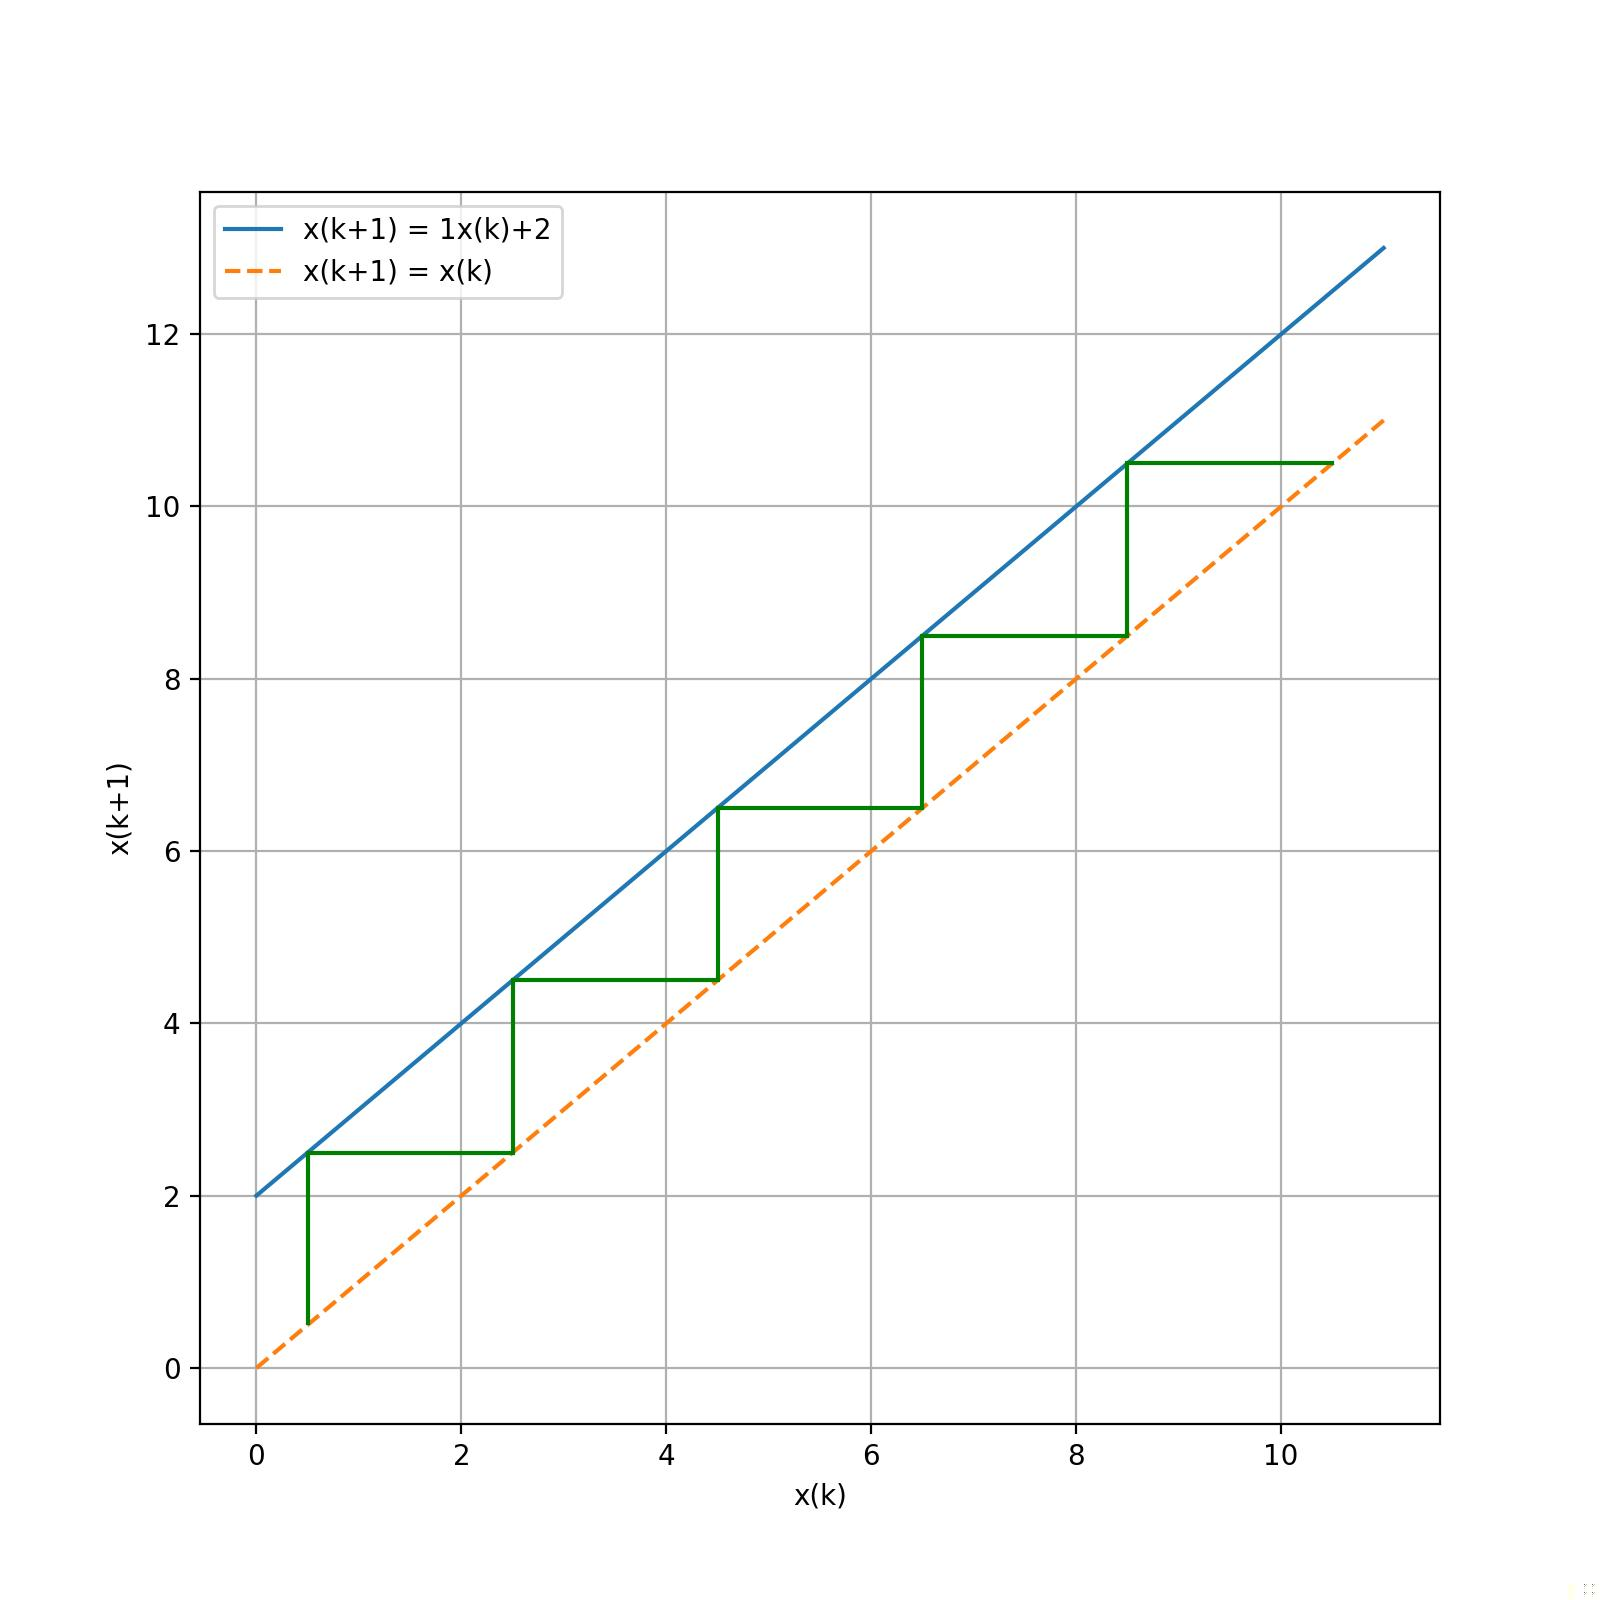
\includegraphics[width=\textwidth]{images/affine_1.jpg}
                \caption{Équation affine à un pas à trajectoire divergente}
                \label{fig:affine_1}
            \end{figure}
            Ensuite, dans la figure \ref{fig:affine_2}, on montre un cas convergent, où $a=0.75$ et $b=2$.
            \begin{figure}[ht!]
                \centering
                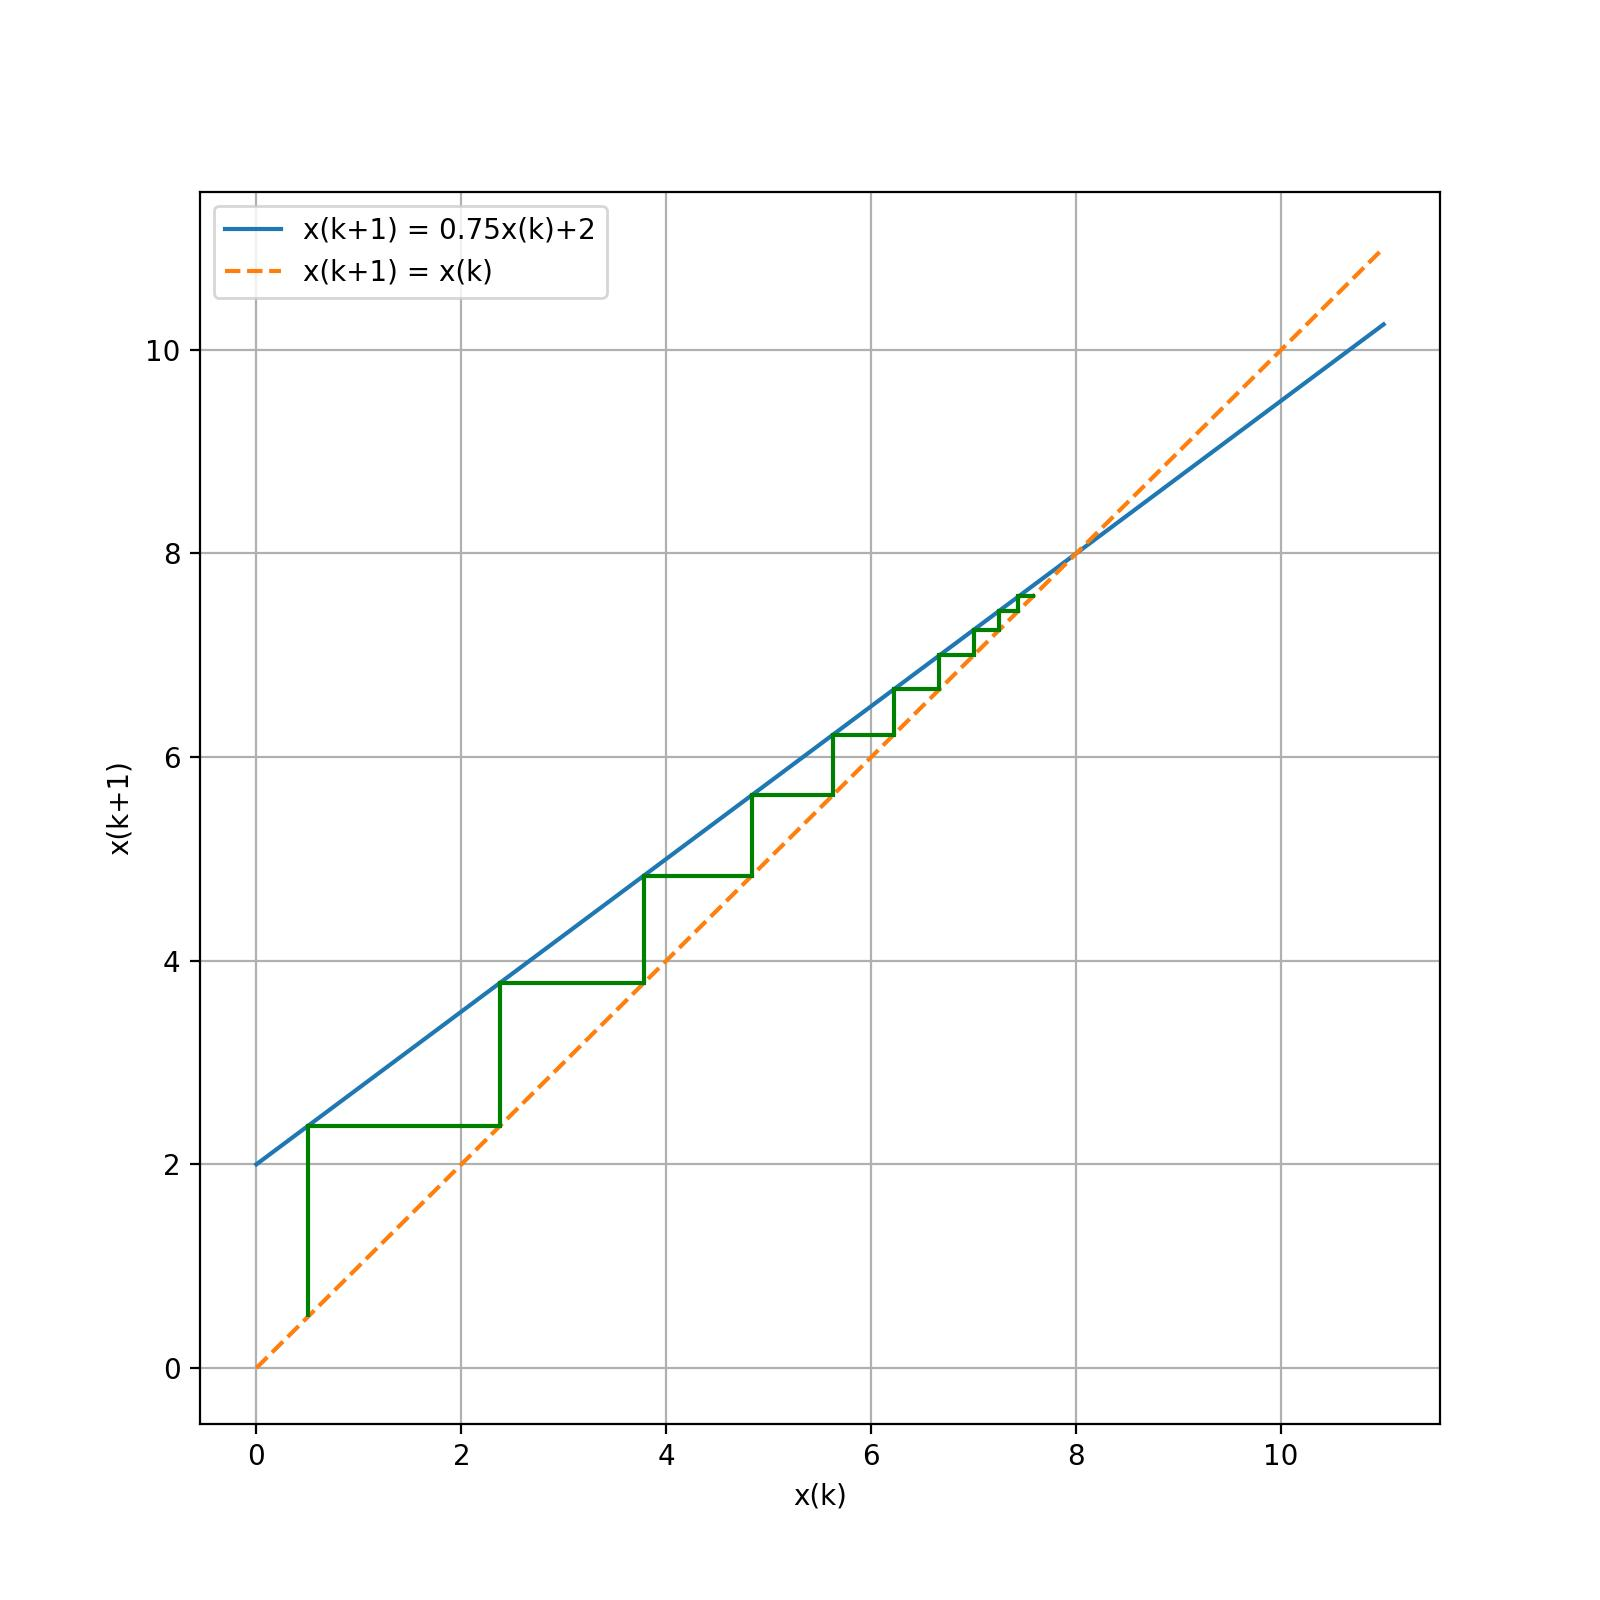
\includegraphics[width=\textwidth]{images/affine_2.jpg}
                \caption{Équation affine à un pas à trajectoire convergente}
                \label{fig:affine_2}
            \end{figure}
            Et on montre finalement dans la figure \ref{fig:affine_3} un cas oscillant, où $a=-0.5$ et $b=8$.
            \begin{figure}[ht!]
                \centering
                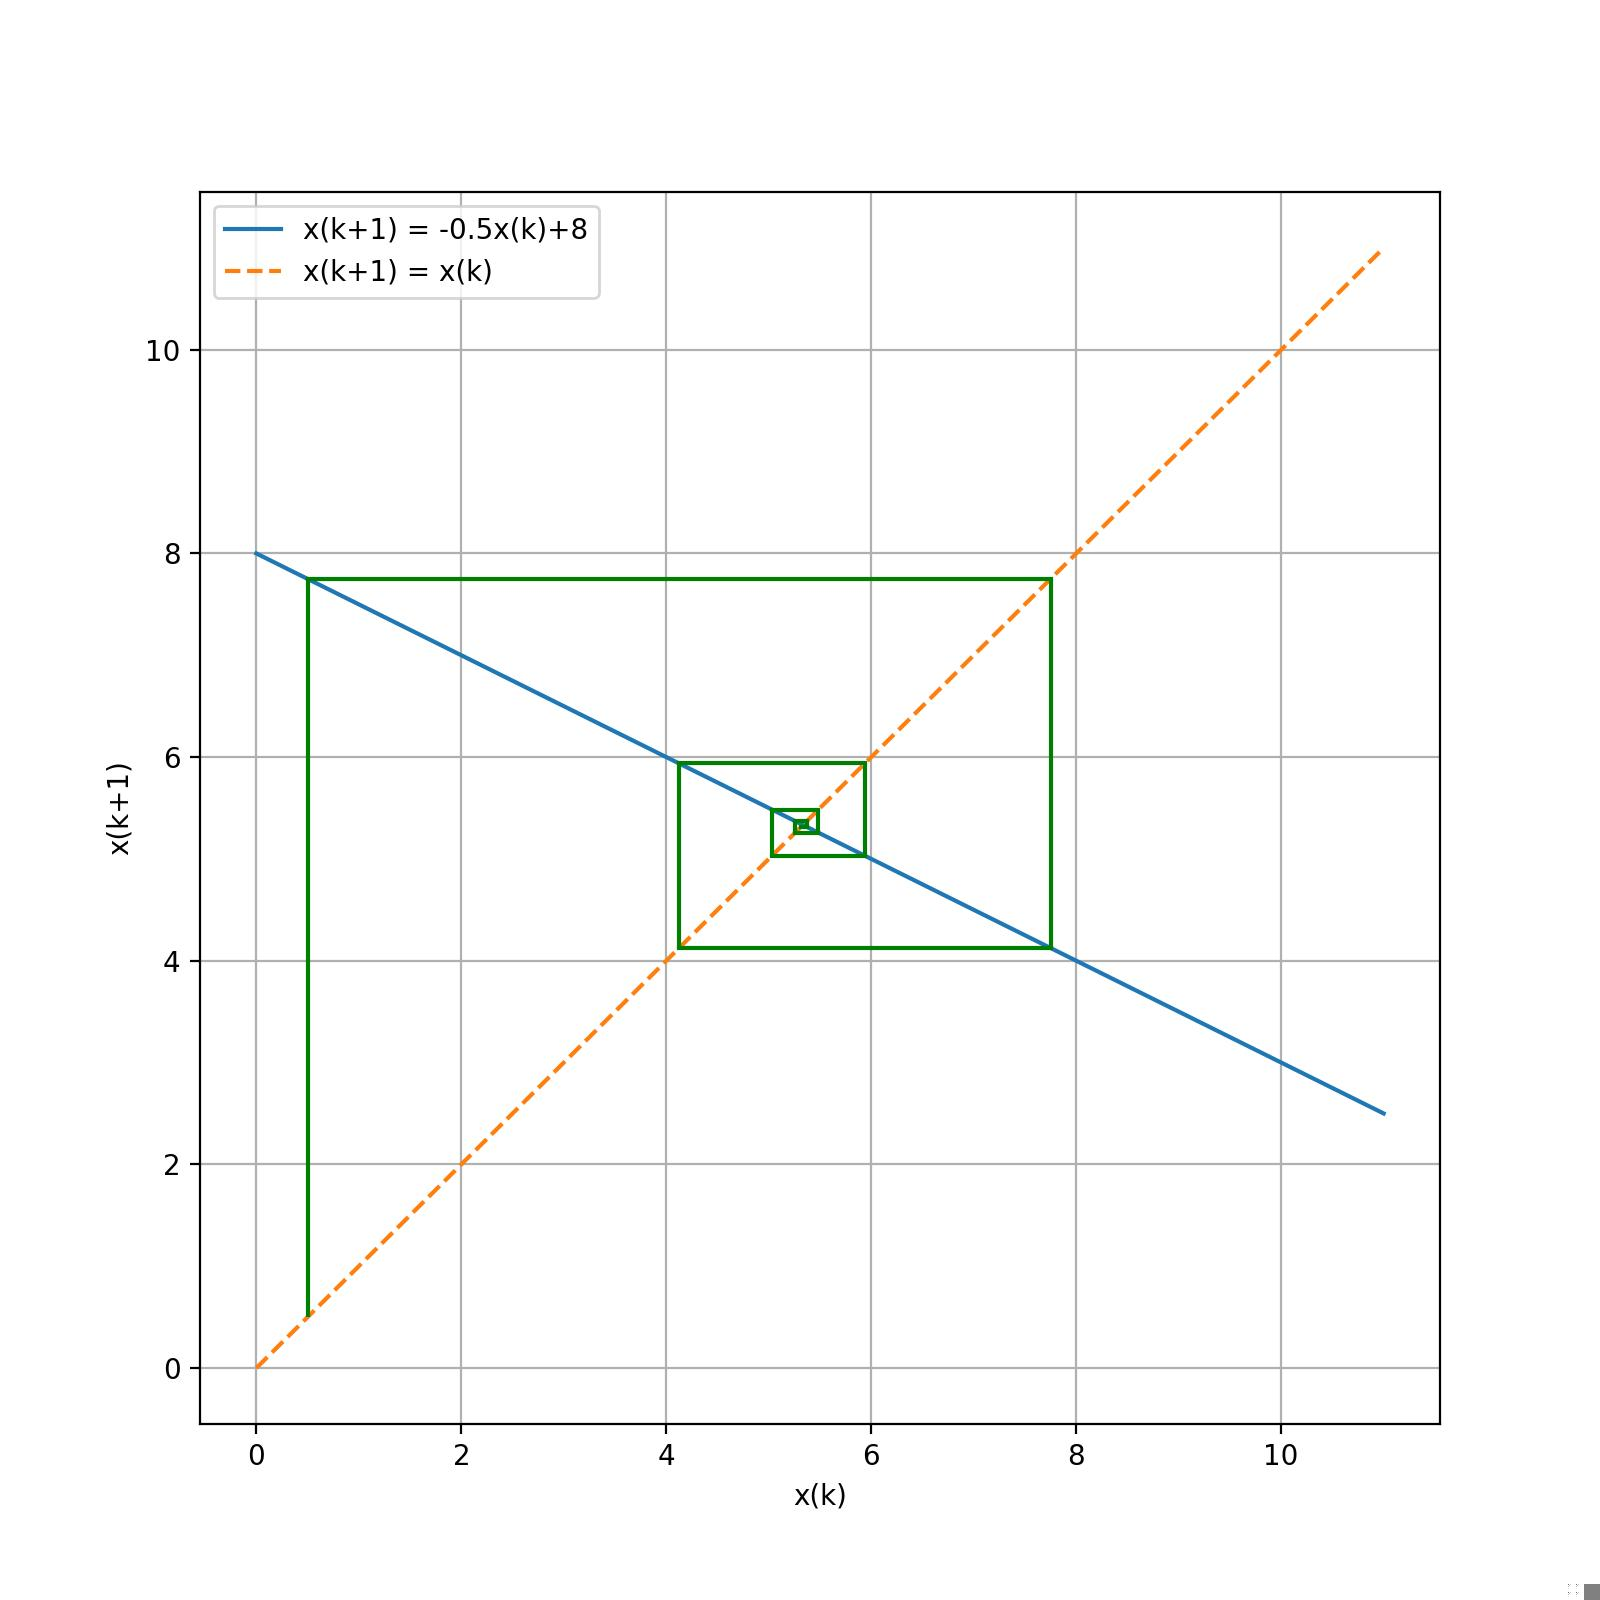
\includegraphics[width=\textwidth]{images/affine_3.jpg}
                \caption{Équation affine à un pas à trajectoire oscillante}
                \label{fig:affine_3}
            \end{figure}
            
    \section{Équations non-linéaires à un pas}
        La méthode graphique montrée précédemment illustre le principe de composition sous-jacent: la projection de la solution $x(k+1)$ sur la droite $x(k+1)=x(k)$ équivaut à reprendre la fonction $x(k+1)$ sur la valeur calculée. Analytiquement, la méthode se traduit par les étapes suivantes:
        \begin{itemize}
            \item on fixe une condition initiale $x(0)$~;
            \item on calcule la première itération: $x(1) = ax(0)+b$~;
            \item pour calculer l'itération qui suit, on utilise la valeur $x(1)$ calculée, c'est-à-dire $ax(0)+b$~;
            \item le résultat s'obtient en composant la relation avec elle-même: $x(2) = a(ax(0)+b)+b$~;
            \item le processus se répète pour les itérations qui suivent.
        \end{itemize}
        Cette méthode s'applique indépendamment de la forme de l'équation, elle peut être utilisée dans le cas non-linéaire de la même manière. Par exemple, dans la figure \ref{fig:un_pas_2}, on montre l'évolution du système décrit par l'équation $x(k+1) = \cos(x(k))$. Le code pour obtenir le graphique est donné:
        \inputminted{python}{codes/un_pas.py}
        \begin{figure}[ht!]
            \centering
            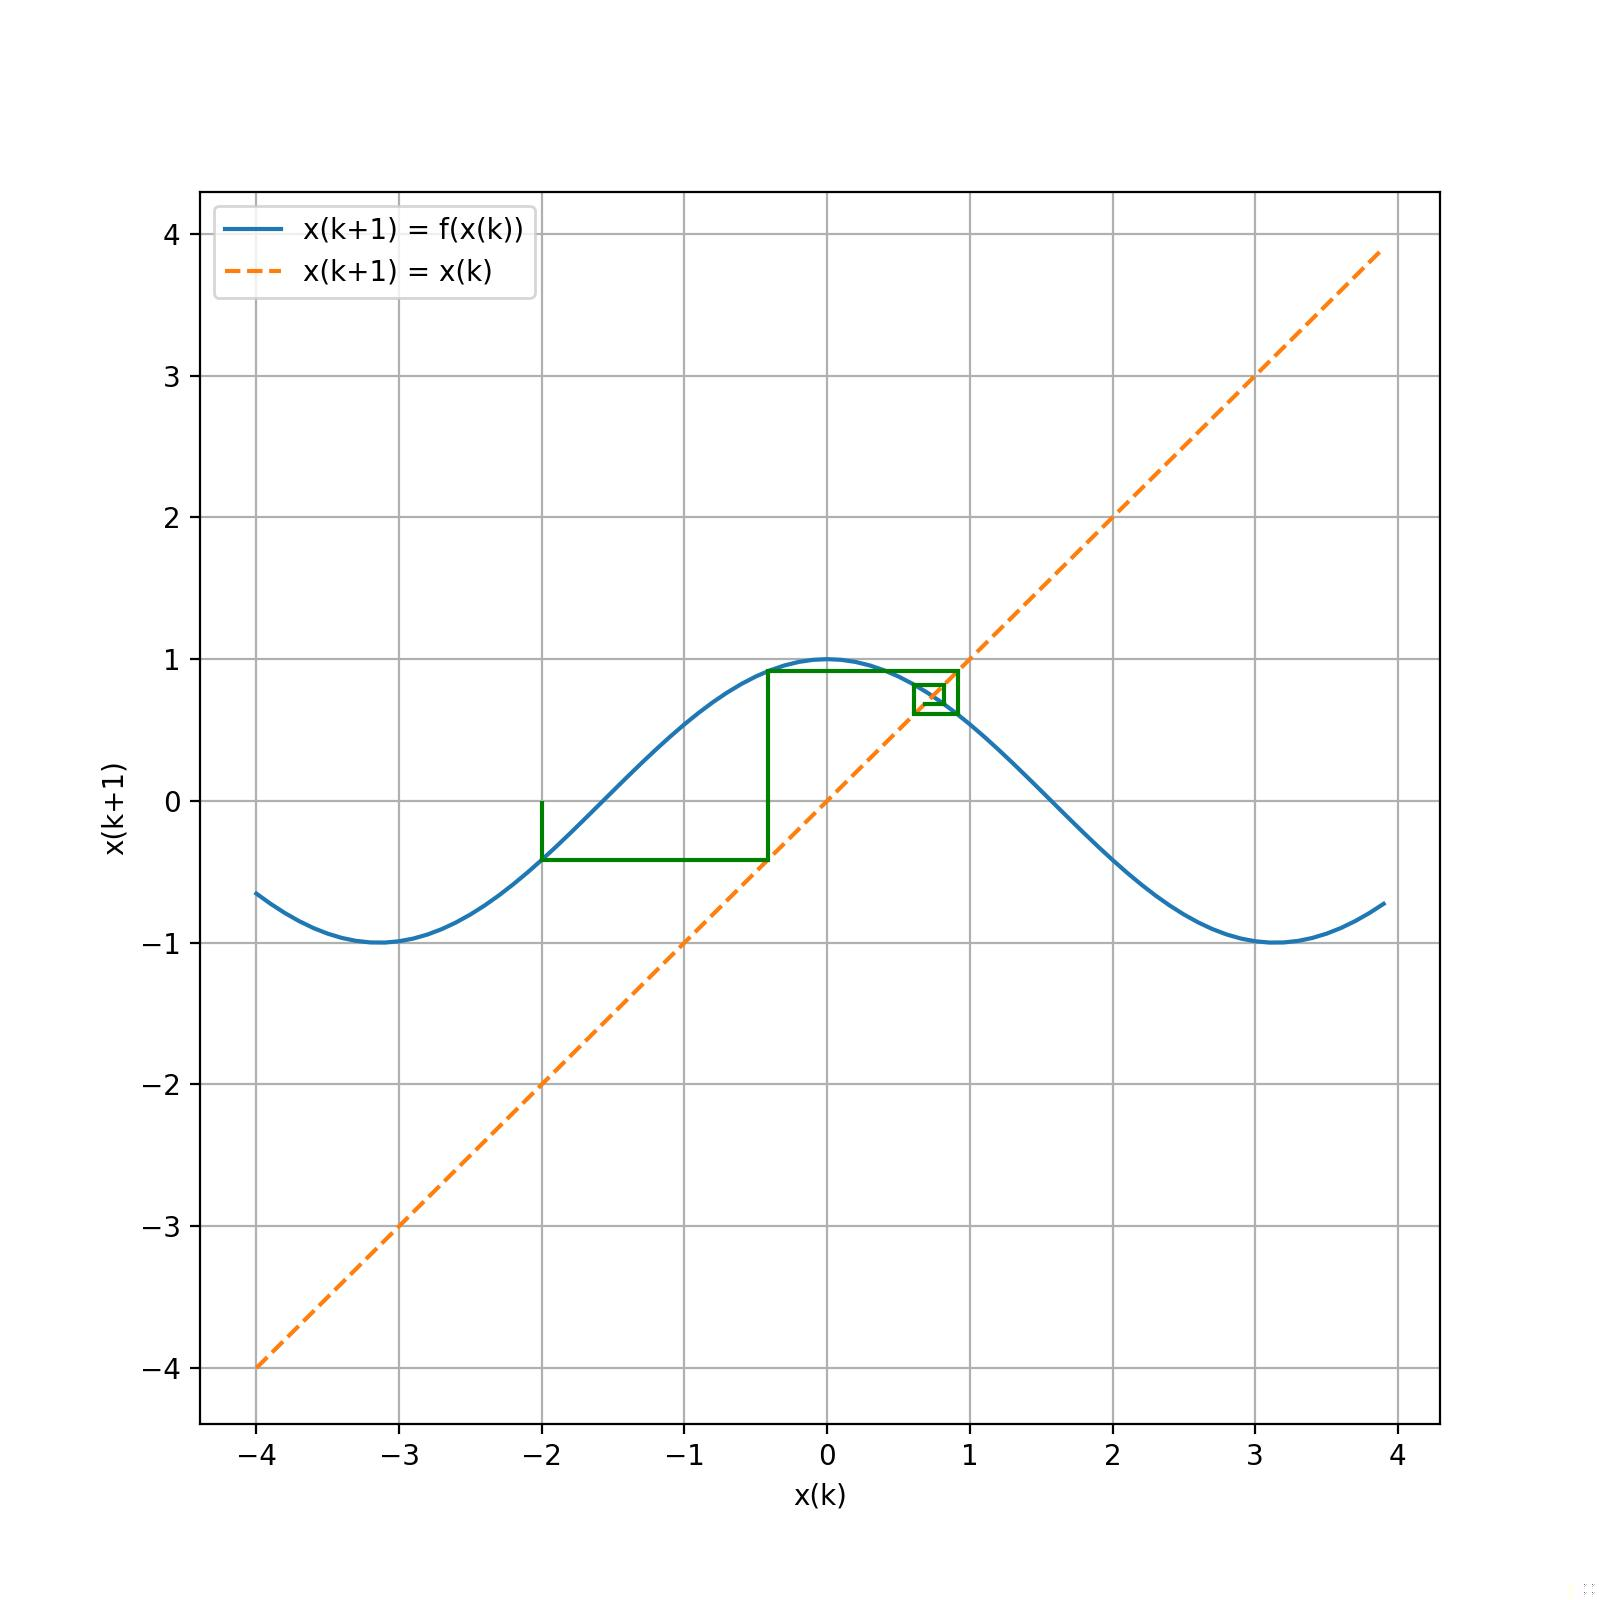
\includegraphics[width=\textwidth]{images/un_pas_2.jpg}
            \caption{Équation non-linéaire à un pas}
            \label{fig:un_pas_2}
        \end{figure}
        Cette notion de composition peut être formalisée avec la notation exponentielle: comme $x(k+1) = f(x(k))$, on peut noter 
        \begin{equation}
            \begin{split}
                x(1) = f(x(0)) \\
                x(2) = f(f(x(0))) = f^2(x(0)) \\
                \dots\\
                x(n) = f(f(\dots f(x(0)))) = f^n(x(0))
            \end{split}
        \end{equation}
        Attention à la notation. Distinguons $f^n(x)$, la \textit{$n^e$ composée de $f$}, $(f(x))^n$, la \textit{$n^e$ puissance de $f$} et $f^{(n)}(x)$, la \textit{$n^e$ dérivée de $f$}. \robin{Et évidemment on garde les notations $\cos^k$, $\sin^k$, $\log^k$, etc. pour les puissances et pas pour la composition sinon ce serait trop simple\ldots}

    \section{États d'équilibre}
        Comme dans le cas à temps continu, les points fixes ou états d'équilibre jouent un rôle important dans la description de la dynamique des systèmes.

        \begin{definition}{État d'équilibre}
            L’état $\bar{x}$ est un état d’équilibre (ou point fixe) du système $\{f, I\}$ \robin{Tu n'as pas défini la notion de \emph{système} (et à nouveau un ensemble n'est pas top, une paire ordonnée est mieux définie)} si
            \begin{equation}
                \bar{x} = f(\bar{x})
            \end{equation}
        \end{definition}
        D'un point de vue géométrique, les points d’équilibre sont les intersections sur le plan $x, y$ entre la fonction $y = f(x)$ et la droite $y = x$.
        \begin{theorem}{Existence d'un point d'équilibre}
            Soit $I = [a, b]$ un intervalle clos et borné et $f : I \to I$ une fonction continue. Alors, il existe toujours un point d’équilibre $\bar{x} \in I$ tel que $f(\bar{x}) = \bar{x}$.
        \end{theorem}

        Par exemple, le système à temps discret décrit par
        \begin{equation}
            x(k + 1) = x(k)^3
        \end{equation}
        a les points fixes $\bar{x}_1 = 0$, $\bar{x}_2 = 1$, $\bar{x}_3 = -1$. Il suffit de vérifier que la composition de la fonction par elle-même pour ces valeurs donne effectivement une valeur fixe.

    \subsection{Stabilité de l'équilibre dans les cas du premier ordre}
        \begin{definition}{Équilibre stable}
            L'équilibre est stable si pour chaque $\epsilon > 0$ il existe une constante $\delta > 0$ telle que \robin{Il manque ton quantificateur sur $k$ quelque part}
            \begin{equation}
                |x(0) - \bar{x}| < \delta \Rightarrow |x(k) - \bar{x}| < \epsilon
            \end{equation}
        \end{definition}
        \begin{definition}{Équilibre globalement asymptotiquement stable}
            L'équilibre est globalement asymptotiquement stable (ou globalement attractif) si pour chaque $x(0) \in I$
            \begin{equation}
                \lim_{k \to \infty} x(k) = \bar{x}
            \end{equation}
        \end{definition}
        \begin{definition}{Équilibre localement asymptotiquement stable}
            L'équilibre est localement asymptotiquement stable (ou localement attractif) s'il existe $\eta > 0$ telle que pour chaque $x(0) \in I \cap [\bar{x} - \eta, \bar{x} + \eta]$ 
            \begin{equation}
                \lim_{k \to \infty} x(k) = \bar{x}
            \end{equation}
        \end{definition}

        \subsection{Cycles}
            \begin{definition}{Cycle d'ordre $n$}
                Soit donné un système discret $\{f, I\}$. Un cycle d'ordre $s$ est un ensemble de $s$ valeurs différentes $\{\bar{x}_0, \dots, \bar{x}_{s-1}\}$ telles que
                \begin{equation}
                    \bar{x}_1 = f(\bar{x}_0), \quad \bar{x}_2 = f(\bar{x}_1), \dots, \quad \bar{x}_0 = f(\bar{x}_{s-1})
                \end{equation}
            \end{definition}
            La quantité $s$ est la période de l’orbite. Par exemple, le système non linéaire $\left\{ \frac{1}{x}, (0, +\infty) \right\}$ a un seul équilibre mais un nombre infini de trajectoires de période $2$.
        
            \begin{theorem}{Condition d'existence d'un cycle}
                Considérons le système discret $\{f, I\}$. La paire $\{\bar{x}_0, \bar{x}_1\}$ est un cycle d'ordre $2$ si et seulement si $\bar{x}_0$ et $\bar{x}_1$ sont des points d'équilibre de $\{f^2, I\}$ mais pas de $\{f, I\}$.
            \end{theorem}
            Par exemple, le système à temps discret
            \begin{equation}
                x(k + 1) = \frac{(2 - x(k))(3x(k) + 1)}{2}
            \end{equation}
            a un cycle d’ordre $3$ formé par les valeurs $\bar{x}_0 = 0$, $\bar{x}_1 = 1$, $\bar{x}_2 = 2$.
        \subsection{Conditions de stabilité}
        \begin{theorem}{Conditions de stabilité}
            Si $\bar{x}$ est un équilibre du système $\{f, I\}$, où $f \in C^1(I)$, alors
            \begin{itemize}
                \item $|f'(\bar{x})| < 1 \Rightarrow \bar{x}$ est localement asymptotiquement stable,
                \item $|f'(\bar{x})| > 1 \Rightarrow \bar{x}$ est instable,
                \item $|f'(\bar{x})| = 1$ ne renvoie aucune information sur la stabilité de $\bar{x}$.
            \end{itemize}
        \end{theorem}
        \begin{theorem}{Équilibre asymptotiquement stable d'une part et stable d'autre part}
            Soit $\bar{x}$ un équilibre du système $\{f, I\}$, où $f \in C^2(I)$ et $f'(\bar{x}) = 1$. Alors
            \robin{Inférieurement/supérieurement asymptotiquement (in)stable pas définis.}
            \begin{itemize}
                \item $f''(\bar{x}) > 0 \Rightarrow \bar{x}$ est inférieurement asymptotiquement stable et supérieurement instable (ou répulsif),
                \item $f''(\bar{x}) < 0 \Rightarrow \bar{x}$ est supérieurement asymptotiquement stable et inférieurement instable (ou répulsif).
            \end{itemize}
        \end{theorem}
        \begin{theorem}{Équilibre instable ou localement asymptotiquement stable}
            Soit $\bar{x}$ un équilibre du système $\{f, I\}$, où $f \in C^3(I)$, $f'(\bar{x}) = 1$ et $f''(\bar{x}) = 0$. Alors
            \begin{itemize}
                \item $f'''(\bar{x}) > 0 \Rightarrow \bar{x}$ est instable,
                \item $f'''(\bar{x}) < 0 \Rightarrow \bar{x}$ est localement asymptotiquement stable.
            \end{itemize}
            
            Soit $\bar{x}$ un équilibre du système $\{f, I\}$, où $f \in C^3$, $f(\bar{x}) = \bar{x}$ et $f'(\bar{x}) = -1$. Alors
            \begin{itemize}
                \item $2f'''(\bar{x}) + 3 (f''(\bar{x}))^2 > 0 \Rightarrow \bar{x}$ est localement asymptotiquement stable,
                \item $2f'''(\bar{x}) + 3 (f''(\bar{x}))^2 < 0 \Rightarrow \bar{x}$ est instable.
            \end{itemize}
        \end{theorem}

    \section{Exercice} 
        \begin{exercise}{Exercice}
            Trouver les cycles \robin{d'ordre 2~?} du système suivant :
            \begin{equation}
                x(k + 1) = x(k)^2 - 1
            \end{equation}
        \end{exercise}
        \begin{enumerate}
            \item Trouver les points d’équilibre du système $\{f, I\}$ :  
            Nous devons résoudre l’équation 
            \begin{equation}
                x = x^2 - 1,
            \end{equation}
            c'est-à-dire
            \begin{equation}
                x^2 - x - 1 = 0,
            \end{equation}
            dont le discriminant $\Delta$ vaut $5$, et dont les racines sont 
            \begin{equation}
                x_{1,2} = \frac{1 \pm \sqrt{5}}{2}.
            \end{equation}
            \item Trouver les points d’équilibre du système $\{f^2, I\}$, nous avons
            \begin{equation}
                f^2 = (x^2 - 1)^2 - 1 = x^4 - 2x^2 + 1 - 1 = x^4 - 2x^2.
            \end{equation}
            Nous devons donc résoudre l’équation 
            \begin{equation}
                x^4 - 2x^2 - x = 0.
            \end{equation}
            Les solutions $0$ et $-1$ sont évidentes, ce qui nous donne la factorisation
            \begin{equation}
                x(x + 1)(x^2 - x - 1) = 0.
            \end{equation}
            L’équation $x^2 - x - 1 = 0$ a déjà été résolue ci-dessus, et a pour racines 
            \begin{equation}
                \frac{1 \pm \sqrt{5}}{2}.
            \end{equation}
            Nous avons donc 
            \begin{equation}
                \bar{x}_0 = 0, \quad \bar{x}_1 = -1, \quad \bar{x}_2 = \frac{1 + \sqrt{5}}{2}, \quad \bar{x}_3 = \frac{1 - \sqrt{5}}{2}.
            \end{equation}
            Les points $\bar{x}_0 = 0$ et $\bar{x}_1 = -1$ sont donc des points d’équilibre de $f^2$ mais pas de $f$. Ils forment donc un cycle d’ordre $2$ du système $\{f, I\}$.
        \end{enumerate}
    \section{Fonction logistique discrète}
        Le système logistique est un système caractérisé par une fonction de transition paramétrique
        \begin{equation}
            x(k + 1) = f_a(x(k)) = a x(k)(1 - x(k)), \quad a \in [0, 4], \quad x \in [0, 1]
        \end{equation}
        Malgré sa simplicité, le système peut afficher des comportements qualitativement très complexes au fur et à mesure que $a$ augmente.
        Le graphique de $f_a$ est une parabole ayant pour origine le point $\left(\frac{1}{2}, \frac{a}{4}\right)$, concave et symétrique par rapport à la droite verticale $x = \frac{1}{2}$.
        Les points fixes sont obtenus en résolvant l’équation
        \begin{equation}
            a x (1 - x) = x
        \end{equation}
        Les racines sont $ \bar{x}_1 = 0 $ et le point $\bar{x}_2 = \frac{a - 1}{a}$ pour $1 < a \leq 4$.
        Notons aussi que les trajectoires ayant comme conditions initiales $x(0) = 1$ \robin{$f_a(1) = 0$. C'est $x(0)=0$} et $x(0) = \frac{1}{a}$ sont constantes pour $k \geq 1$.
        Au fur et à mesure que le paramètre $a$ augmente, le comportement qualitatif du système change fortement.
        Afin de l’analyser, il est important de tenir en considération que
        \begin{equation}
            f(x) = a x (1 - x), \quad f'(x) = a - 2 a x, \quad f''(x) = -2 a, \quad f'''(x) = 0
        \end{equation}

        \subsection{Équilibre stable: $0 \leq a < 1$}
            Si $a \in [0, 1)$, le point d'équilibre $\bar{x}_1 = 0$ est le seul équilibre. Puisque $|f'(0)| = a < 1$, il est stable. Un exemple pour $a=0.5$ est donné en Figure \ref{fig:logistique_differences_1}.
            \begin{figure}[ht!]
                \centering
                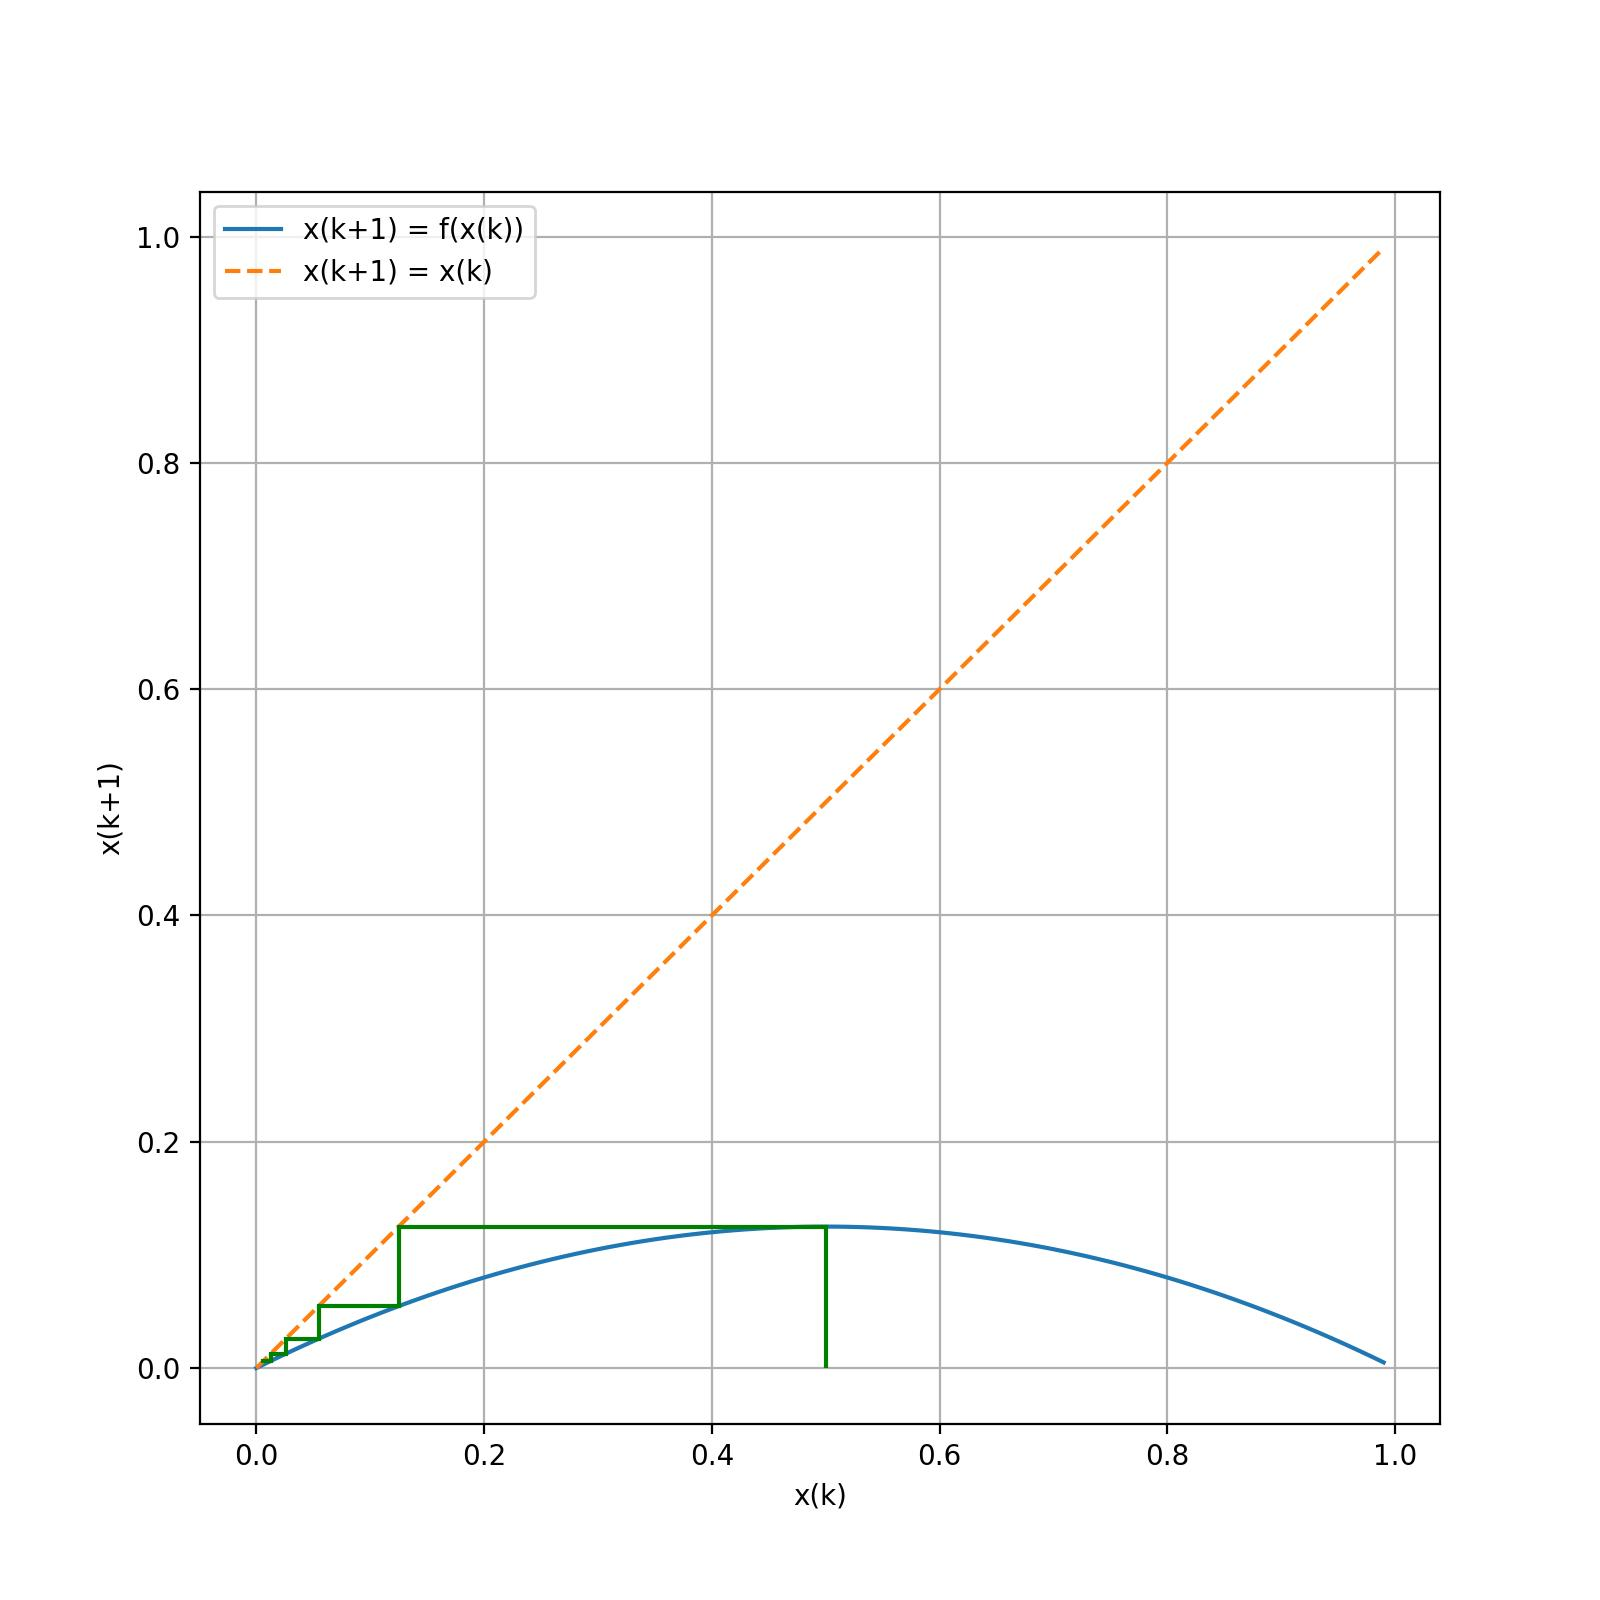
\includegraphics[width=\textwidth]{images/logistique_differences_1.jpg}
                \caption{Équation logistique pour $a=0.5$}
                \label{fig:logistique_differences_1}
            \end{figure}
            
        \subsection{Équilibre asymptotiquement stable: $a = 1$}
            Si $a = 1$, puisque $|f'(0)| = a = 1$ et $f''(0) = -2a < 0$, l'équilibre $\bar{x}_1 = 0$ est supérieurement asymptotiquement stable. Un exemple pour $a=1$ est donné en Figure \ref{fig:logistique_differences_2}.
            \begin{figure}[ht!]
                \centering
                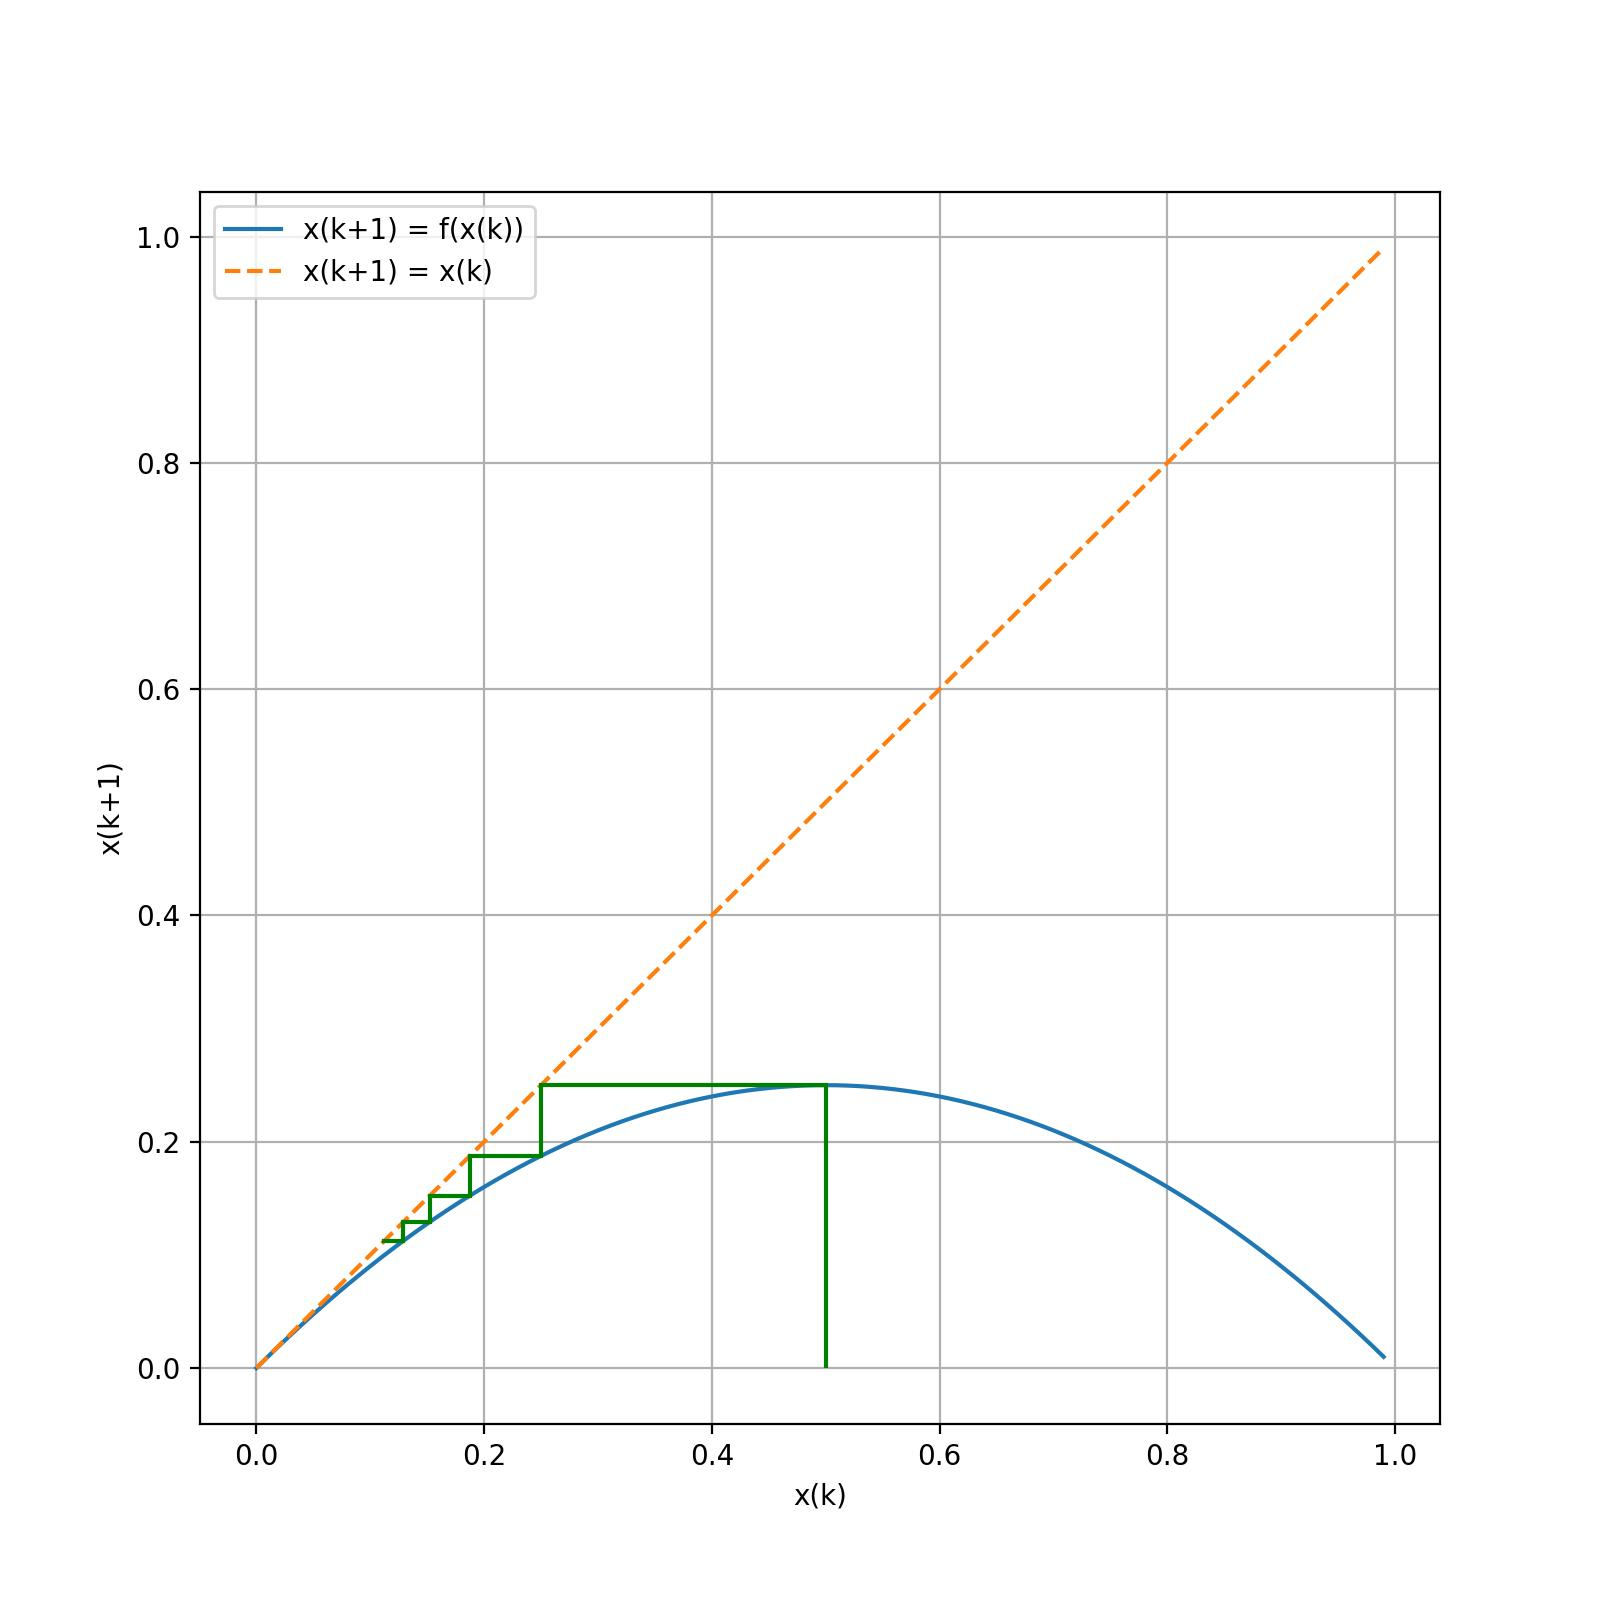
\includegraphics[width=\textwidth]{images/logistique_differences_2.jpg}
                \caption{Équation logistique pour $a=1$}
                \label{fig:logistique_differences_2}
            \end{figure}

        \subsection{Équilibre localement asymptotiquement stable, ou instable: $1 < a < 4$}
            \begin{itemize}
                \item Si $1 < a \leq 4$, nous avons deux points fixes : $\bar{x}_1 = 0$ et $\bar{x}_2 = \frac{a - 1}{a}$.
                \item Puisque $|f'(0)| = a > 1$, le point $\bar{x}_1 = 0$ est instable.
                \item Puisque $|f'(\bar{x}_2)| = |2 - a|$, l'équilibre $\bar{x}_2$ est stable pour $1 < a < 3$.
                \item Pour $a = 3$, nous avons $f'(\bar{x}_2) = -1$, $f''(\bar{x}_2) = -2a = -6$, $f'''(\bar{x}_2) = 0$. Puisque
                \begin{equation}
                    2f'''(\bar{x}_2) + 3(f''(\bar{x}_2))^2 > 0
                \end{equation}
                alors $\bar{x}_2$ est localement asymptotiquement stable.
                \item L’équilibre $\bar{x}_2$ devient instable pour $3 < a \leq 4$.
            \end{itemize}
            Deux exemples pour $a=1.5$ sont donnés en Figures \ref{fig:logistique_differences_3} et \ref{fig:logistique_differences_4}, pour $x_0=0.1$ et $x_0=0.9$.
            \begin{figure}[ht!]
                \centering
                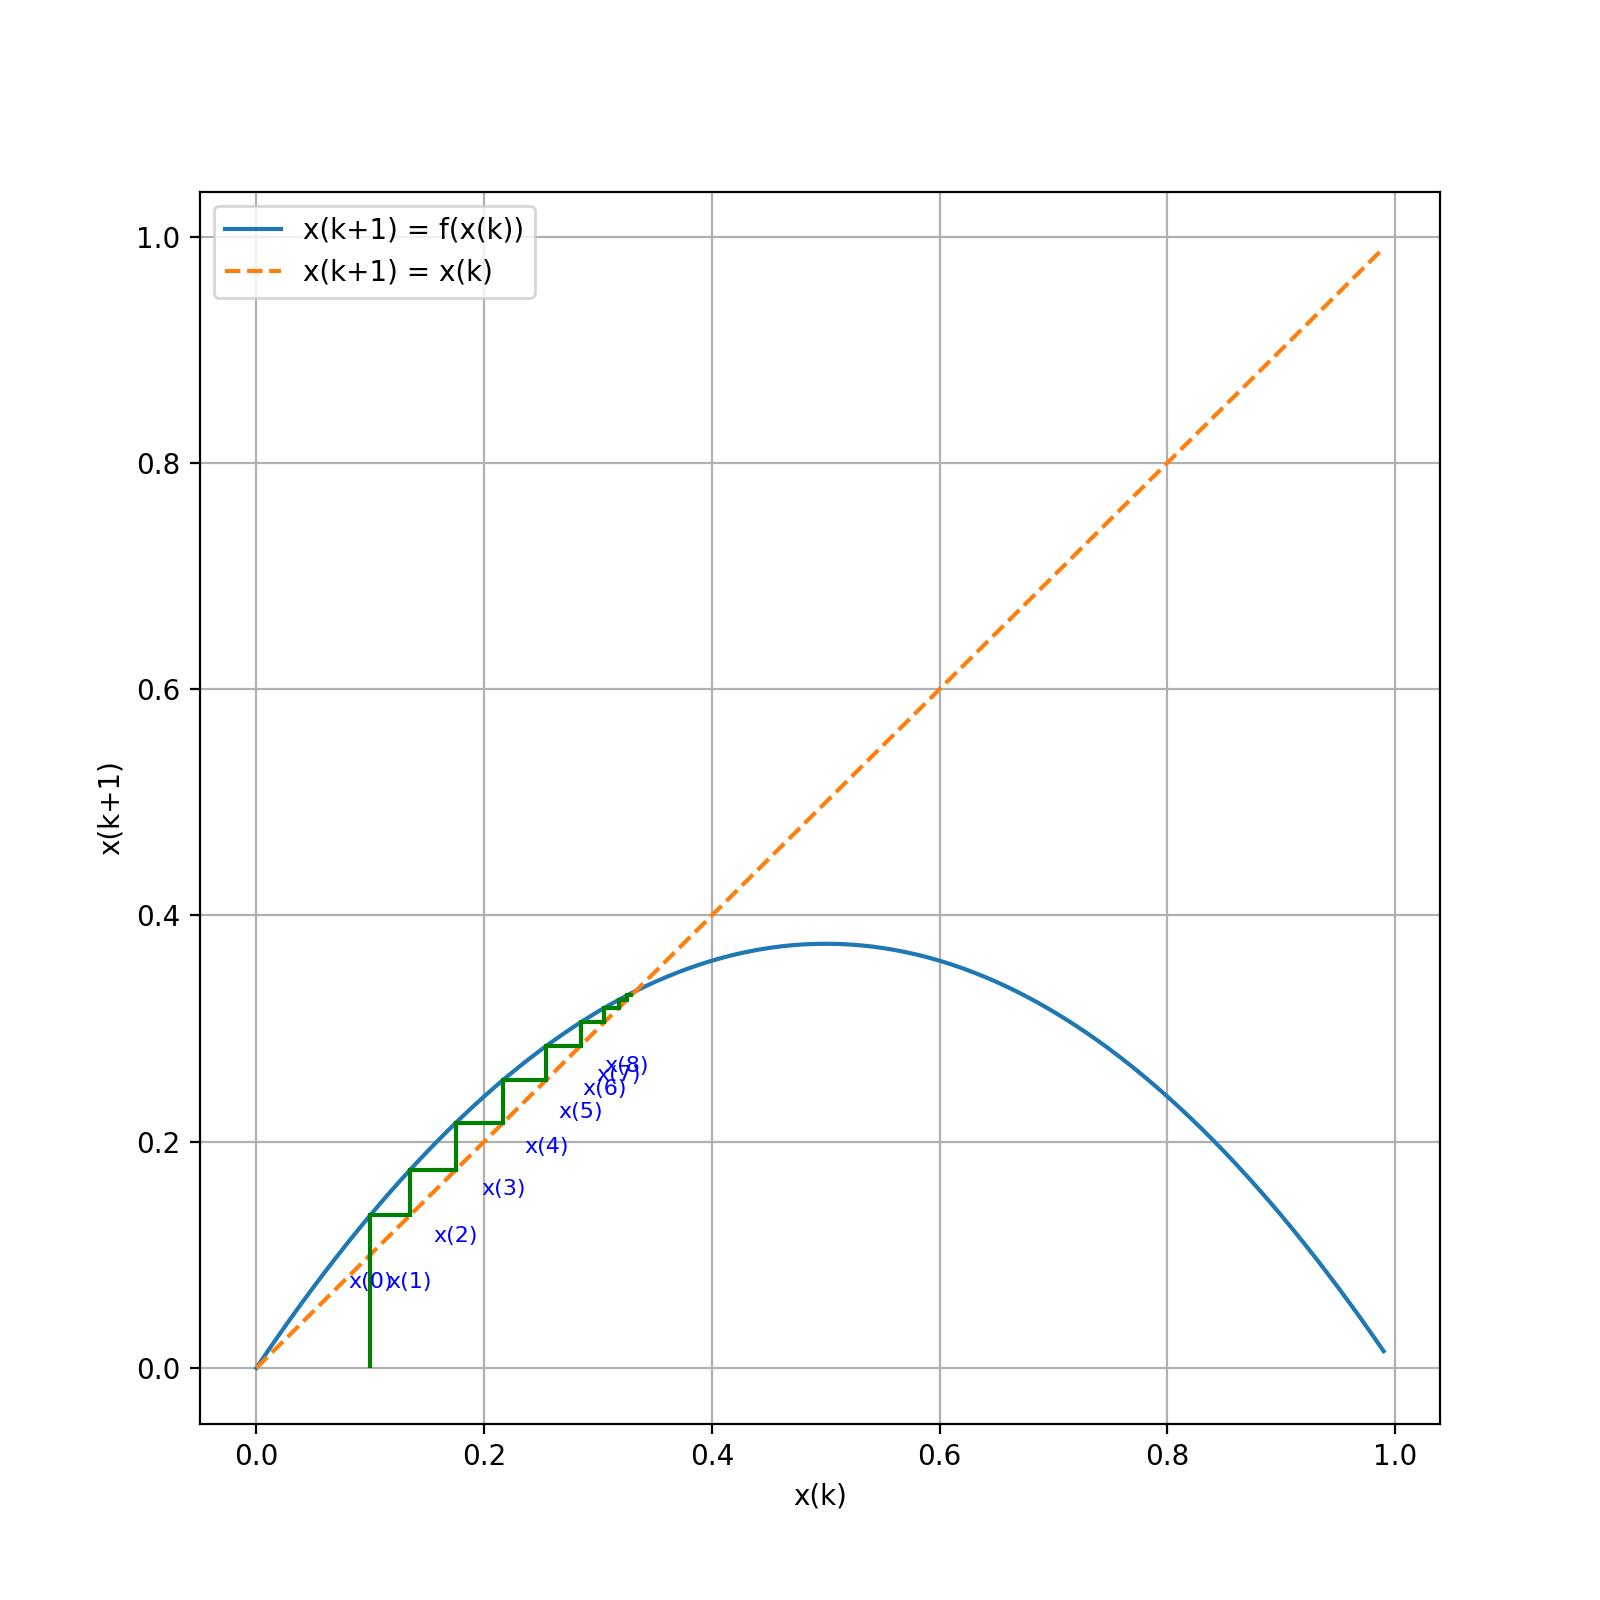
\includegraphics[width=\textwidth]{images/logistique_differences_3.jpg}
                \caption{Équation logistique pour $a=1.5$, $x_0=0.1$}
                \label{fig:logistique_differences_3}
            \end{figure}
            \begin{figure}[ht!]
                \centering
                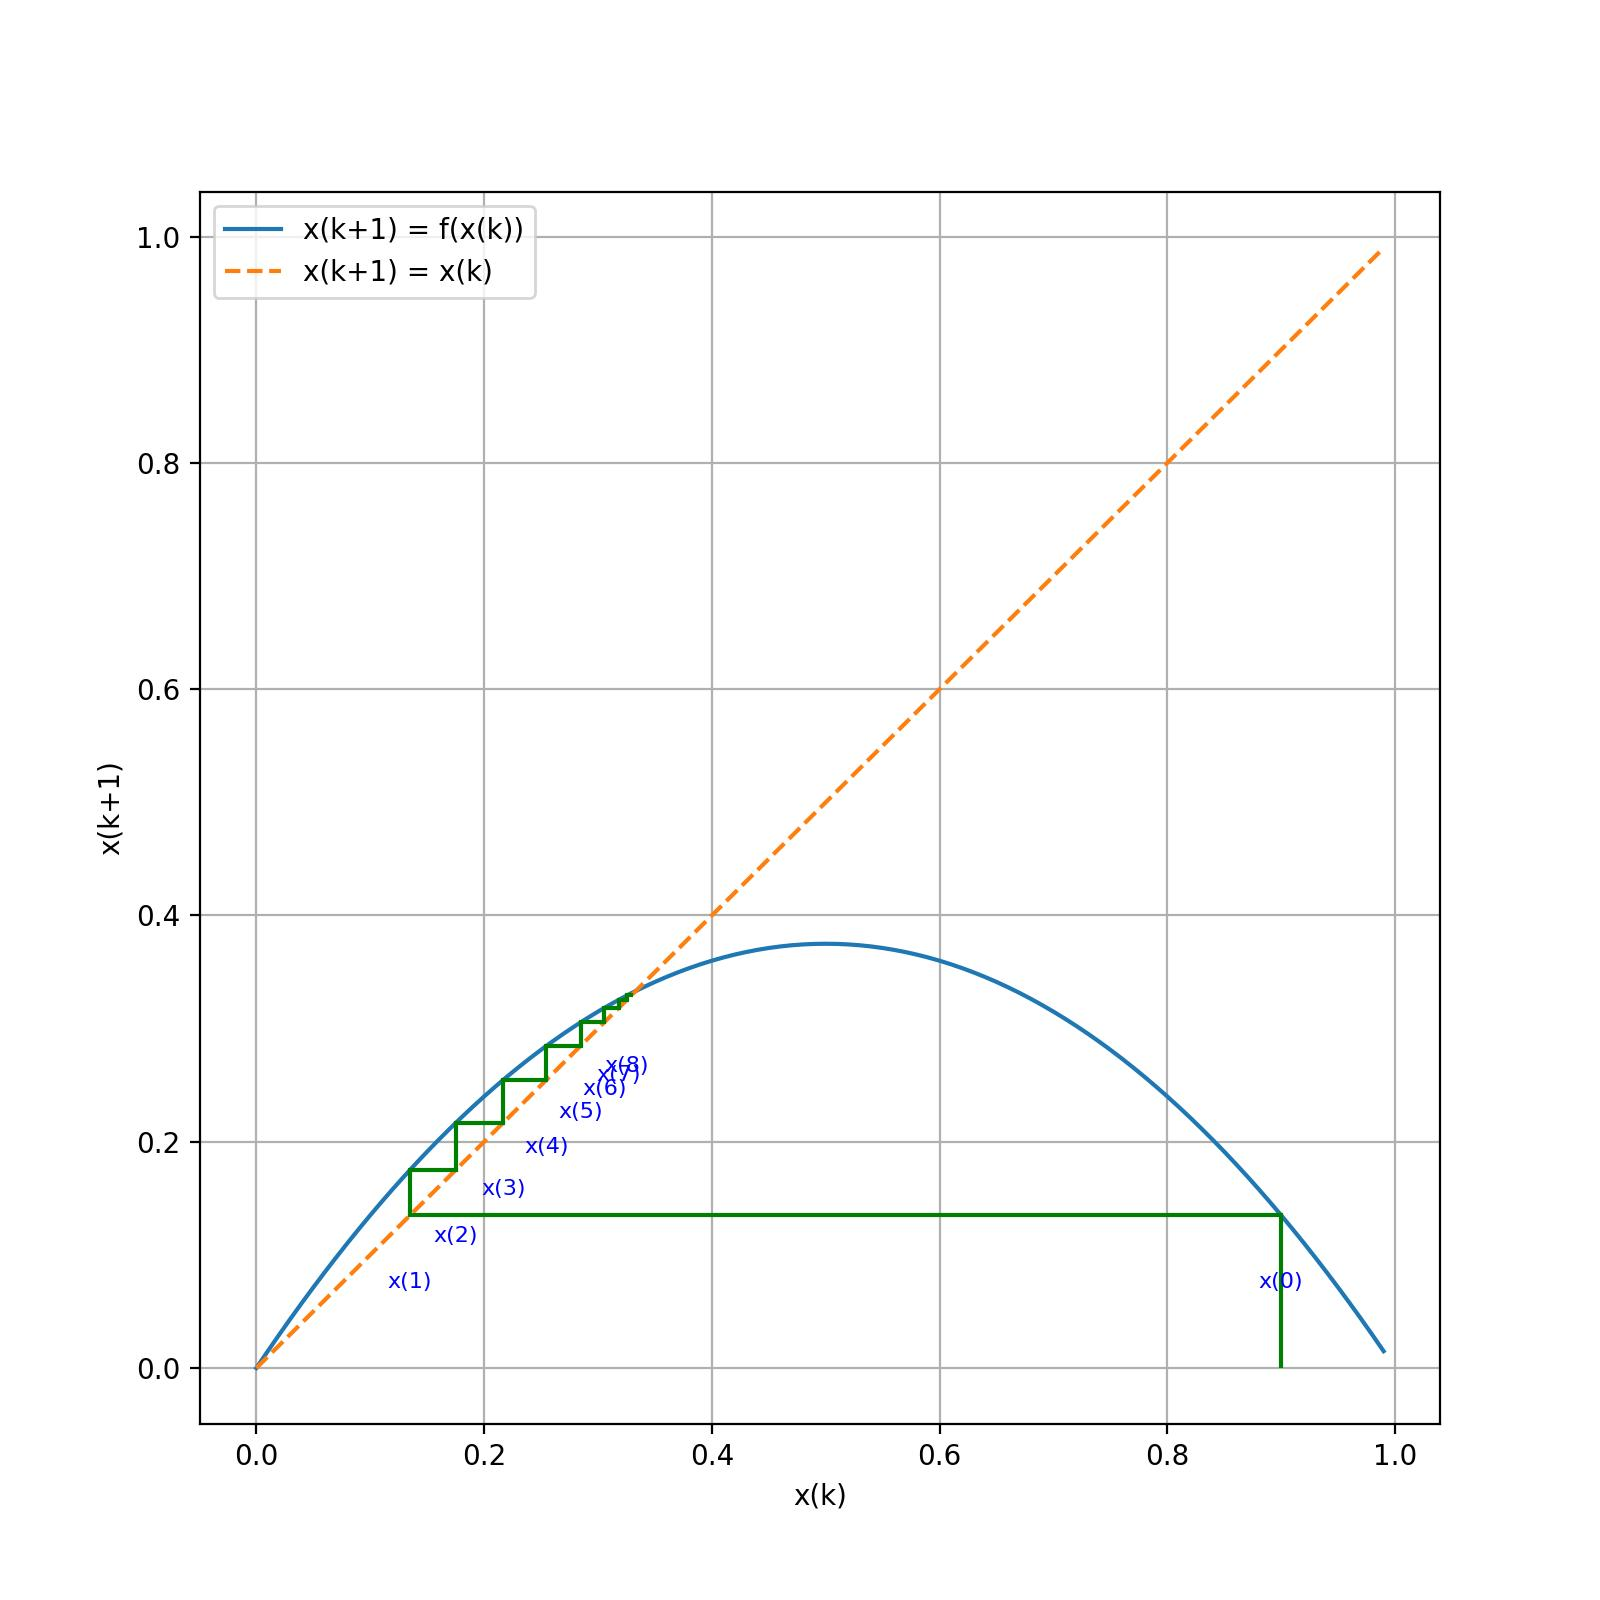
\includegraphics[width=\textwidth]{images/logistique_differences_4.jpg}
                \caption{Équation logistique pour $a=1.5$, $x_0=0.9$}
                \label{fig:logistique_differences_4}
            \end{figure}

            \subsubsection{Exemple: $a = 3$}
                L’équilibre est localement asymptotiquement stable pour $a = 3$.
                Une trajectoire est donnée en Figure \ref{fig:logistique_differences_5}.
                \begin{figure}[ht!]
                    \centering
                    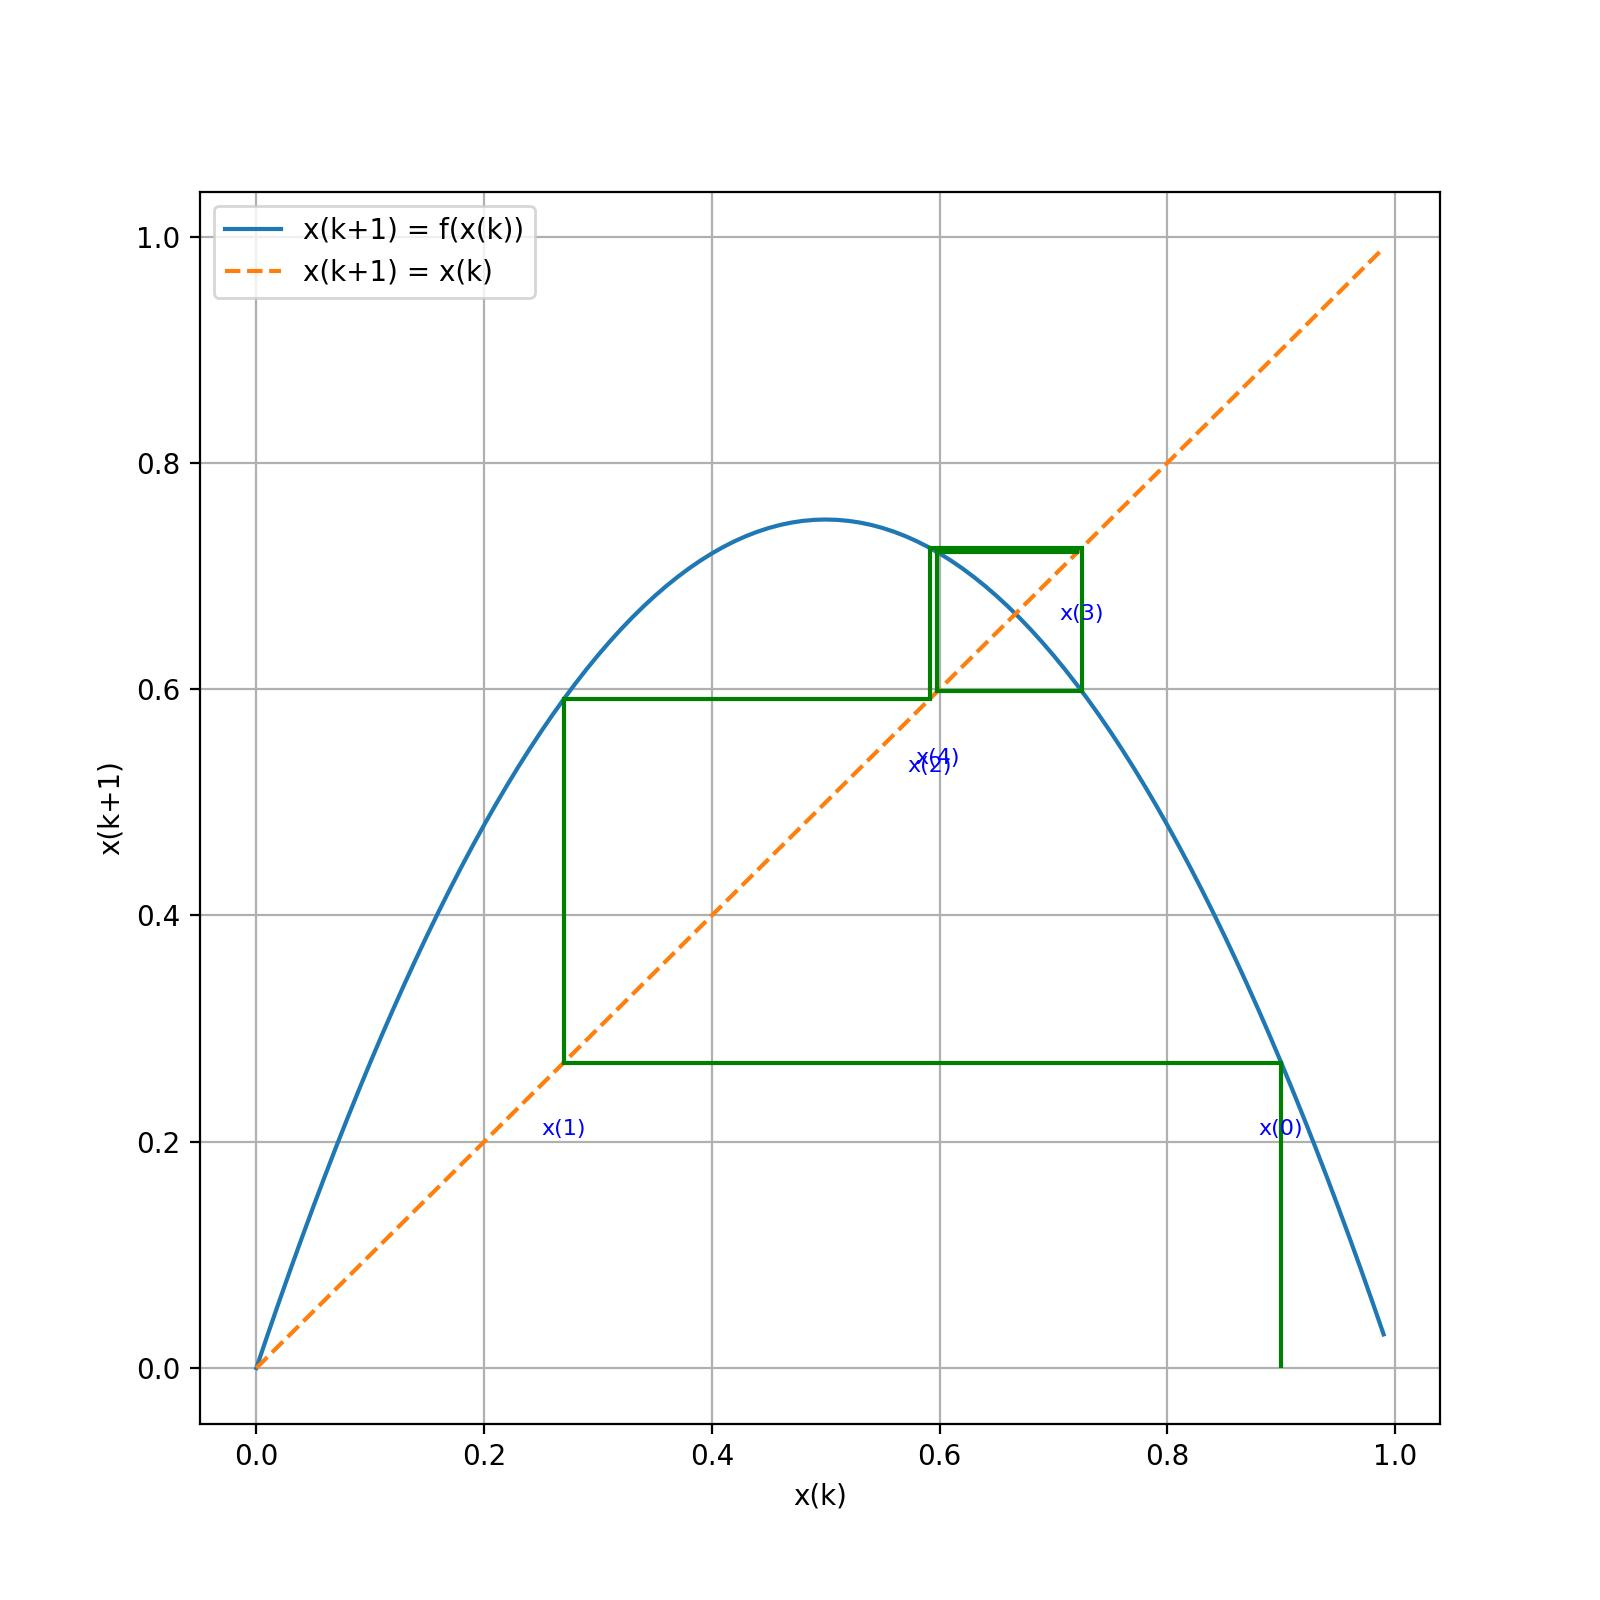
\includegraphics[width=\textwidth]{images/logistique_differences_5.jpg}
                    \caption{Équation logistique pour $a=3$}
                    \label{fig:logistique_differences_5}
                \end{figure}
            
            \subsubsection{Exemple: $a = 3.3$}
                Pour $a = 3.3 < 1 + \sqrt{6}$, l’équilibre est instable pour $3 < a < 4$.
                Un cycle stable d’ordre 2 apparaît. Une trajectoire est donnée en Figure \ref{fig:logistique_differences_6}.
                \begin{figure}[ht!]
                    \centering
                    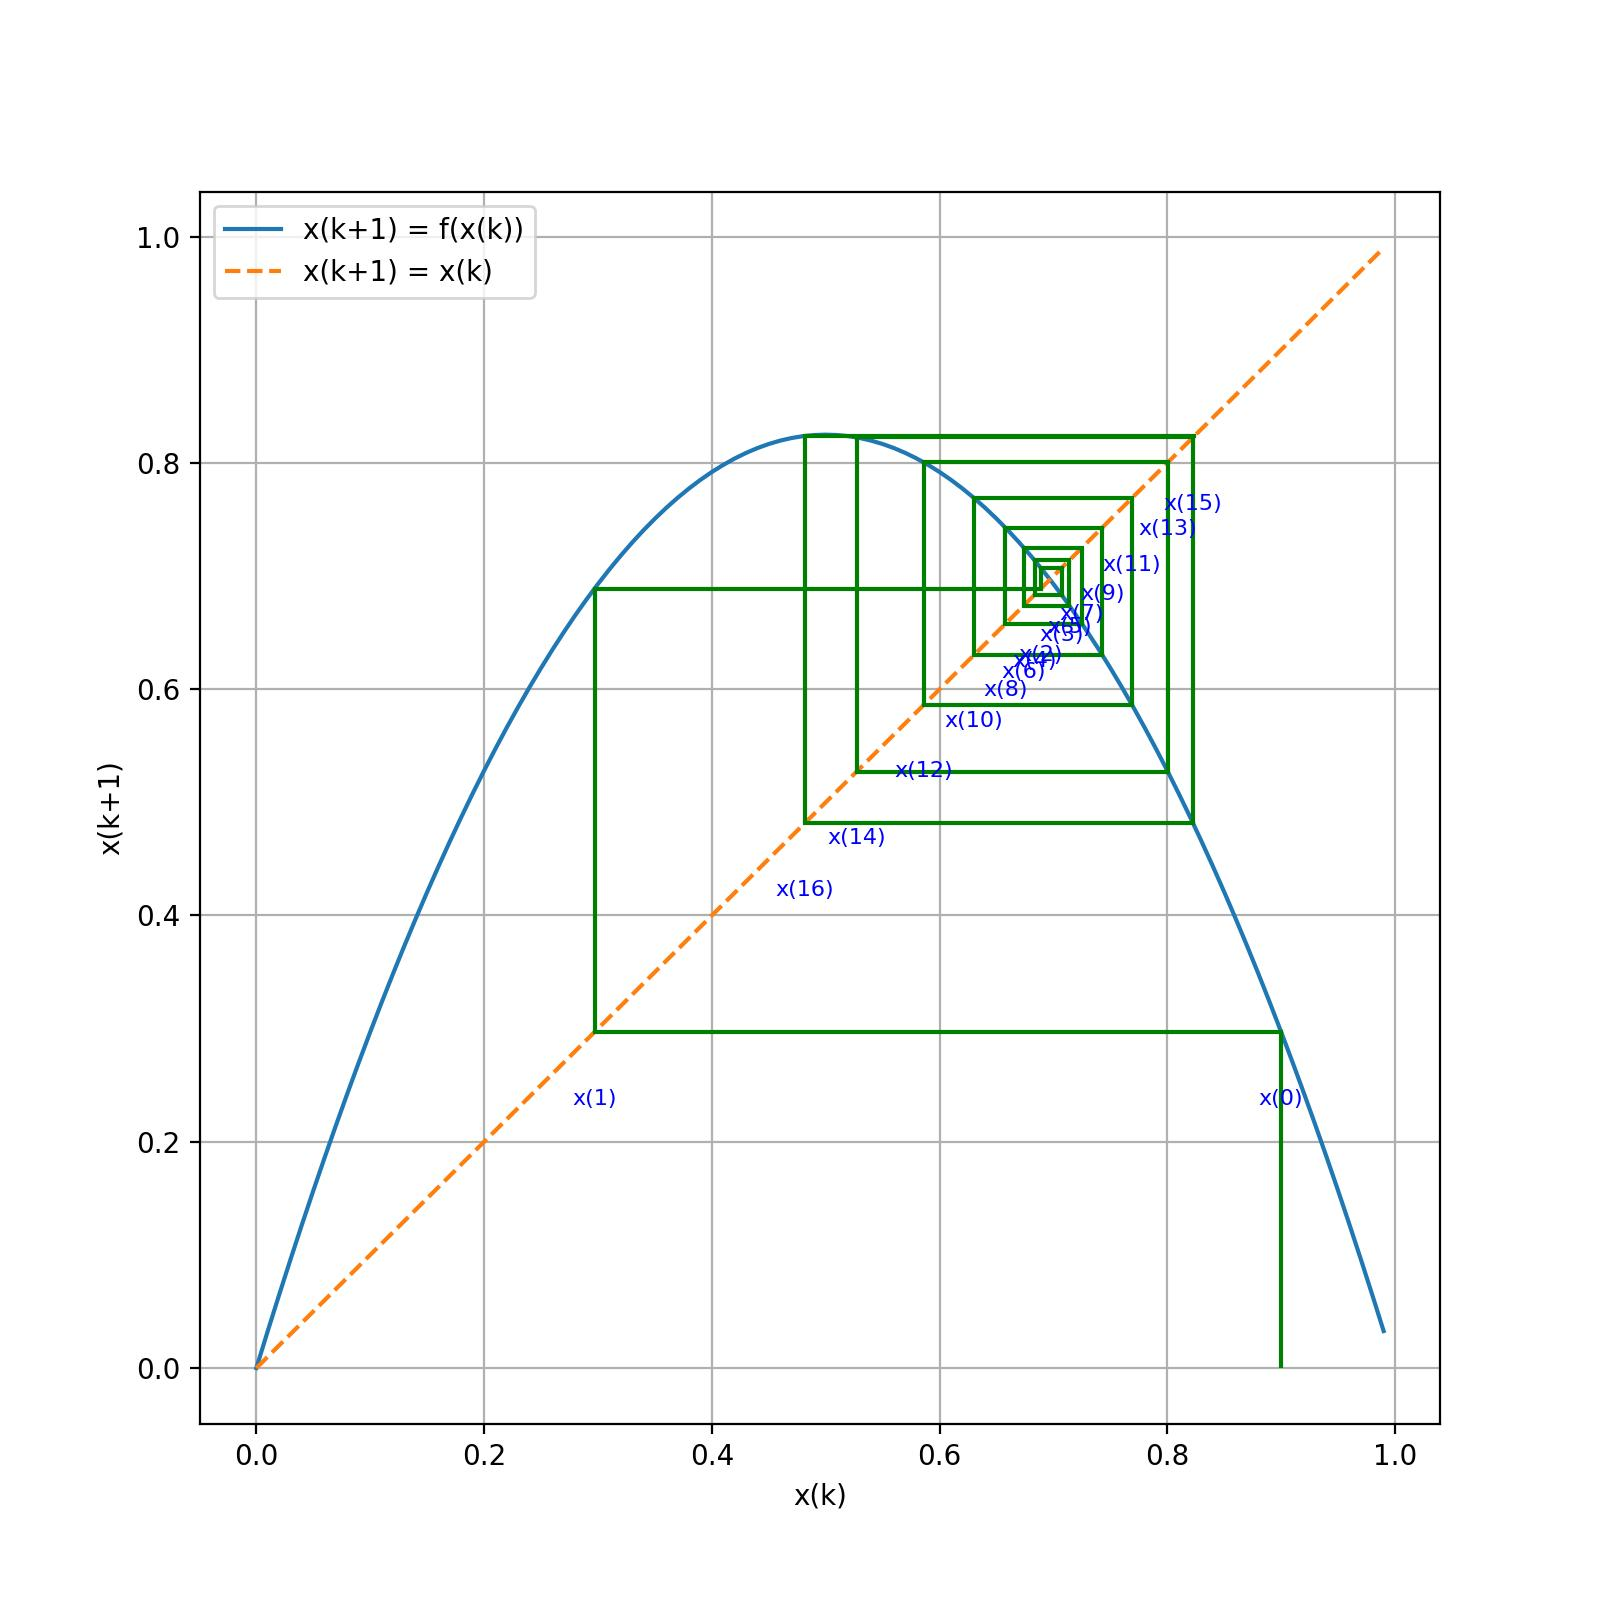
\includegraphics[width=\textwidth]{images/logistique_differences_6.jpg}
                    \caption{Équation logistique pour $a=3.3$}
                    \label{fig:logistique_differences_6}
                \end{figure}
            
                En fait, si $3 < a \leq 4$, un cycle de période $2$ apparaît. Ceci est vérifié par le fait que
                \begin{equation}
                    \begin{split}
                        &f^2(x) = a^2 x(1 - x)(1 - ax(1 - x)) = x \\
                        \Rightarrow& x = \frac{x(a - 1)}{a} \left( -a^3 x^2 + (a^2 + a^3)x - (a^2 + a) \right) = 0
                    \end{split}
                \end{equation}
                qui a quatre solutions distinctes : $\bar{x}_1$, $\bar{x}_2$ et deux solutions additionnelles
                \begin{equation}
                    \beta = \frac{a + 1 + \sqrt{(a - 3)(a + 1)}}{2a}, \quad \gamma = \frac{a + 1 - \sqrt{(a - 3)(a + 1)}}{2a}.
                \end{equation}
\chapter{Simulation Monte Carlo}
    \section{Introduction}
        Les chapitres précédents ont permis à l'étudiant·e de se familiariser avec la simulation de systèmes déterministes, c'est-à-dire de systèmes dans lesquels le comportement peut être univoquement prédit en connaissant les conditions initiales. Dans le cas contraire, le système est dit \textit{stochastique}. De tels systèmes requièrent de nouveaux outils pour étudier leur comportement. Nous présentons une telle méthode, appelée \textit{simulation Monte Carlo}.
        
        Une simulation de Monte Carlo est une méthode statistique utilisée pour estimer le comportement d'un système complexe en modélisant l'incertitude de ses paramètres grâce à des tirages aléatoires. En répétant de nombreuses fois des simulations qui incluent des éléments de hasard, elle permet d'obtenir une approximation de l'impact de ces incertitudes sur les résultats. 
        
        La modélisation du système commence par la définition d'un modèle du problème à étudier, en identifiant les variables et les paramètres d'intérêt. Ensuite, les incertitudes sont représentées par des distributions de probabilité. Par exemple, si un temps avant un évènement varie, cette variation peut être modélisée par une distribution normale, exponentielle, ou autre. Pour chaque simulation, des tirages aléatoires sont effectués pour chaque paramètre incertain, en suivant la distribution définie. En utilisant les valeurs tirées, on simule le comportement du système et on enregistre les résultats. Ce processus est répété un grand nombre de fois afin de capturer un large échantillon de scénarios possibles. Finalement, une analyse statistique est effectuée sur les résultats des simulations pour estimer des métriques telles que la moyenne, l'écart-type, la distribution des résultats, ou des intervalles de confiance.

    \section{Générateur uniforme}
        Nous rappellerons quelques définitions essentielles pour la compréhension de cette section. Cependant, nous référons l'étudiant·e au cours de Probabilités et Statistique (\cite{mathf315_1, mathf315_2}) pour un aperçu plus extensif des notions utiles.

        Le syllabus offre une explication extensive de la nécessité degénérateur de nombres uniformes (\cite{infof305}). Dans cette section, nous proposons des implémentations pour les méthodes expliquées dans le syllabus.
        \subsection{Méthode de Neumann}
            John von Neumann\footnote{John von Neumann était un mathématicien américano-hongrois né en 1903 et décédé en 1957. Ses contributions vont de la mécanique quantique à l'informatique théorique en passant par les sciences économiques. Son intérêt pour le développement de la méthode Monte Carlo date de la période de la Seconde Guerre Mondiale. Il a notamment participé au projet Manhattan.} a proposé, en étudiant les simulations Monte Carlo, qui nécessitaient bien entendu une méthode pour générer des nombres pseudo-aléatoires, la méthode qui a donné son nom(\cite{von195113}). Le code suivant en montre une implémentation.
            \inputminted{python}{codes/von_neumann.py}
            Cependant, lorsque le système atteint l'état $0$, il reste bloqué, c'est un état absorbant. 
            
        \subsection{Générateur congruentiel linéaire}
            Rapidement après la méthode proposée par von Neumann, Lehmer\footnote{Derrick Lehmer était un mathématicien américain né en 1905 et décédé en 1991. Ses contributions concernent principalement des problèmes d'analyse et de théorie des nombres, pour lesquel il fut un pionnier dans l'utilisation d'ordinateurs et de méthodes numériques. Notamment, il travailla avec sa femme Emma Markovna Trotskaya comme opérateur sur l'ENIAC, le premier ordinateur Turing-complet entièrement éléctronique.} proposa un autre algorithme pour la génération de nombre suivant une distribution pseudo-aléatoire uniforme (\cite{lehmer1951}). Nous en montrons une implementation dans le code suivant.
            \inputminted{python}{codes/LGC.py}
            
        \subsection{Test de \textit{randomness}}
            Afin de vérifier si les générateurs de nombres pseudo-aléatoires que nous avons présentés sont fiables, en pratique, il est possible de réaliser des tests statistiques comparant la distribution des échantillons qu'ils produisent avec la distribution uniforme. Nous en présentons quelques implémentations.
            \subsubsection{Test des moments}
                \begin{definition}{Moment brut}
                    Soit un échantillon $x_1, x_2, ..., x_n$ de réalisations d'une variable aléatoire $\mathbf{X}$. Le $n^{\text{ème}}, n \in \mathbb{N_0^+}$ \textbf{moment brut} autour de l'origine de $\mathbf{X}$ est donné par
                    \begin{equation}
                        \mathbb{E}(\mathbf{X}^n) = \int_{-\infty}^{+\infty} x^n f(x) \, dx
                    \end{equation}
                    
                    Sa valeur peut être estimé par la fonction
                    \begin{equation}
                        \hat{m}_k = \frac1n \sum_{i=0}^n x_i^k
                    \end{equation}
                \end{definition}
                Ainsi, on peut vérifier si les générateurs proposés pour la distribution uniforme sur $[0, 1]$ respectent les moments attendus. Le code suivant montre que le générateur congruentiel linéaire vérifie ce test.
                \inputminted{python}{codes/moments_test.py}

            \subsubsection{Test $\chi^2$}
                Si l'on divise l'intervalle $[0, 1]$ en $s$ sous-intervalles de taille égale, et que l'échantillon de taille $N$ que l'on étudie respecte une distribution uniforme, alors, chaque sous-intervalle devrait contenir, en moyenne, $s/N$ éléments. Soit $c_j$ le nombre mesuré d'éléments dans le sous-intervalle $j$. On peut quantifier la quantité
                \begin{equation}
                    C = \frac{s}{N} \sum_{j=1}^s (c_j - \frac{N}{s})^2
                \end{equation}
                qui est une mesure de la concordance entre le nombre d'éléments attendus et le nombre d'éléments mesurés. 

                Si l'échantillon respectent une distribution uniforme, alors la quantité $C$ est distribuée comme une variable $\chi^2$ à $s-1$ degrés de liberté (on réfèrera l'étudiant·e au cours de statistiques (\cite{mathf315_2})). Le module \codeword{scipy.stats} propose une classe \codeword{chi2}. La méthode \codeword{cdf(aC, s)} de cette classe permet d'obtenir la p-value, c'est-à-dire la probabilité sous l'hypothèse nulle d'observer une valeur aussi extrême que celle obtenue. L'hypothèse nulle décrite ici est l'hypothèse d'uniformité. Si cette p-value est en-dessous d'un seuil critique choisi (typiquement, 5\%), alors on rejette l'hypothèse nulle, parce qu'il est très peu probable qu'en vérifiant l'hypothèse on obtienne la valeur observée. Un exemple est donné dans le code suivant.
                \inputminted{python}{codes/chi2_test.py}

            \subsubsection{Goodness of fit}
                \begin{definition}{Fonction de répartition empirique}
                    Soit un échantillon $x_1, x_2, ..., x_N$ \textbf{fonction de répartition empirique} est donnée par
                    \begin{equation}
                        \hat{F}_{\mathbf{X}}(x) = \frac{\#x_i < x}{N}
                    \end{equation}
                \end{definition}

                Intuitivement, le test de Kolmogorov-Smirnov compare cette fonction de répartition empirique avec la fonction de répartition théorique en donnant comme estimation le plus grand écart entre ces deux fonctions. La fonction de répartition d'une distribution uniforme est donnée dans le module \codeword{scipy.stats}, mais l'on laissera l'implémentation complète à l'étudiant·e. Le même module offre une fonction macro \codeword{kstest}. On montre dans le code suivant comment vérifier l'uniformité grâce à ce test.
                \inputminted{python}{codes/goodness_of_fit.py}
            
    \section{Générateur aléatoire}
        Le syllabus démontre déjà comment obtenir certaines distribution en modifiant un échantillon d'une distribution uniforme. Nous renvoyons l'étudiant·e vers la démonstration de la méthode de la transformation inverse, pour les distributions uniforme sur un autre intervalle que $[0, 1]$ et pour une distribution exponentielle.
        \subsection{Méthode de rejet}
            La méthode de rejet, proposée par von Neumann en 1951, permet d'échantillonner une variable aléatoire qui suit une distribution cible $p_{\mathbf{X}}(x)$.
            Nous voulons échantillonner une telle distribution.
            Admettons que nous ayons un générateur de nombre aléatoire qui échantillonne une distribution suivant une densité $q(x)$. Si il existe un nombre $C>0$ tel que $\forall x, Cq(x) \geq p_{\mathbf{X}}(x)$, autrement dit, que $q(x)$ \textit{est strictement supérieure} en tout point à $p_{\mathbf{X}}(x)$, à un facteur près, alors la méthode de rejet est la suivante:
            \begin{itemize}
                \item Échantillonner une valeur $x$ suivant $q(x)$
                \item Échantillonner une valeur $u$ suivant une distribution indépendante de $q(x)$, typiquement, une distribution uniforme $\mathbf{U}(0, 1)$
                \item Renvoyer $x$ si $u \leq \frac{p_{\mathbf{X}}(x)}{C q(x)}$, sinon, recommencer
            \end{itemize}
            Comment calculer le dernier quotient ? La fonction de densité uniforme est de $1$, et la fonction de densité objective est connue. Donc, dans le cas où l'on choisit $q(x)$ uniforme, le quotient est donné par $\frac{p_{\mathbf{X}}(x)}{C}$.
            
            Il va de soi que ce processus fonctionne si il existe une fonction qui recouvre la densité attendue. Par exemple, les générateurs de distribution uniforme proposés précédemment ne pourraient pas être utilisés pour échantillonner une distribution normale, car sa fonction de densité a une enveloppe infinie (pensez aux queues: comment un rectangle fini pourrait les contenir ?).

    \section{Exercices}
        \subsection{Méthode de rejet}
            \subsubsection{Densité carrée}
                \begin{exercise}{Densité carrée}
                    Écrivez le code python permettant d'échantillonner une distribution décrite par la densité suivante, par la méthode de rejet. Vous pouvez utiliser le générateur uniforme proposé par \codeword{numpy.random}.
                    \begin{equation}
                        p(x) = 
                        \begin{cases}
                            x^2 \text{ si $0\leq x\leq 3^{\frac13}$}\\
                            0 \text{ sinon}
                        \end{cases}
                    \end{equation}
                    Vérifiez analytiquement que la distribution suivant cette densité est correctement normalisée.
                \end{exercise}
                Le code suivant montre la solution. En figure \ref{fig:exercice_rejet_1}, on montre l'histogramme de l'échantillon produit par cette méthode.
                \inputminted{python}{codes/exercice_rejet_1.py}
                \begin{figure}[ht!]
                    \centering
                    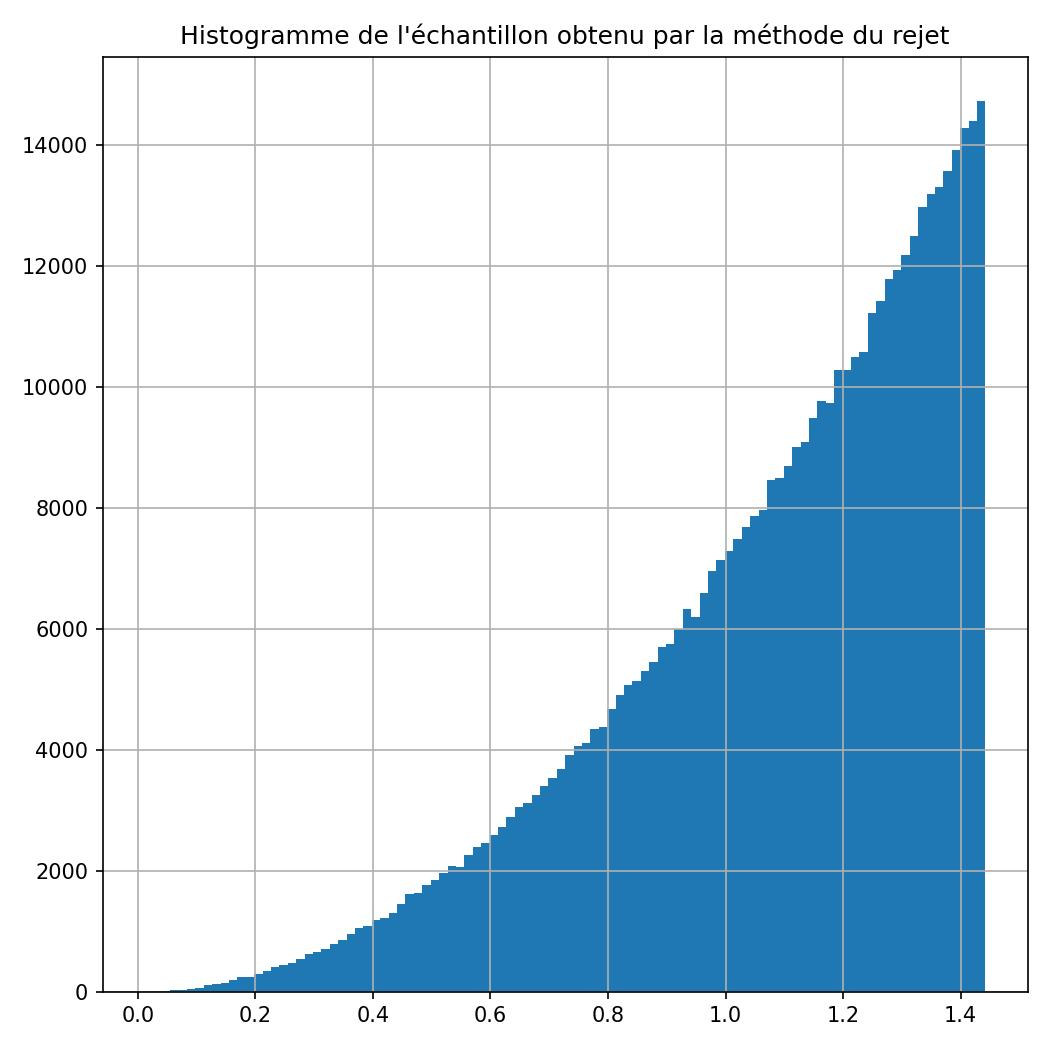
\includegraphics[width=0.7\textwidth]{images/exercice_rejet_1.jpg}
                    \caption{Histogramme de l'échantillon d'une distribution suivant la loi carrée demandée}
                    \label{fig:exercice_rejet_1}
                \end{figure}

            \subsubsection{Densité sinusoïdale}
                \begin{exercise}{Densité carrée}
                    Écrivez le code python permettant d'échantillonner une distribution décrite par la densité suivante, par la méthode de rejet. Vous pouvez utiliser le générateur uniforme proposé par \codeword{numpy.random}.
                    \begin{equation}
                        p(x) = 
                        \begin{cases}
                            \frac{\sin x}{2} \text{ si $0\leq x\leq \pi$ ou si  $2\pi\leq x\leq 3\pi$}\\
                            0 \text{ sinon}
                        \end{cases}
                    \end{equation}
                \end{exercise}
                Le code suivant montre la solution. En figure \ref{fig:exercice_rejet_2}, on montre l'histogramme de l'échantillon produit par cette méthode.
                \inputminted{python}{codes/exercice_rejet_2.py}
                \begin{figure}[ht!]
                    \centering
                    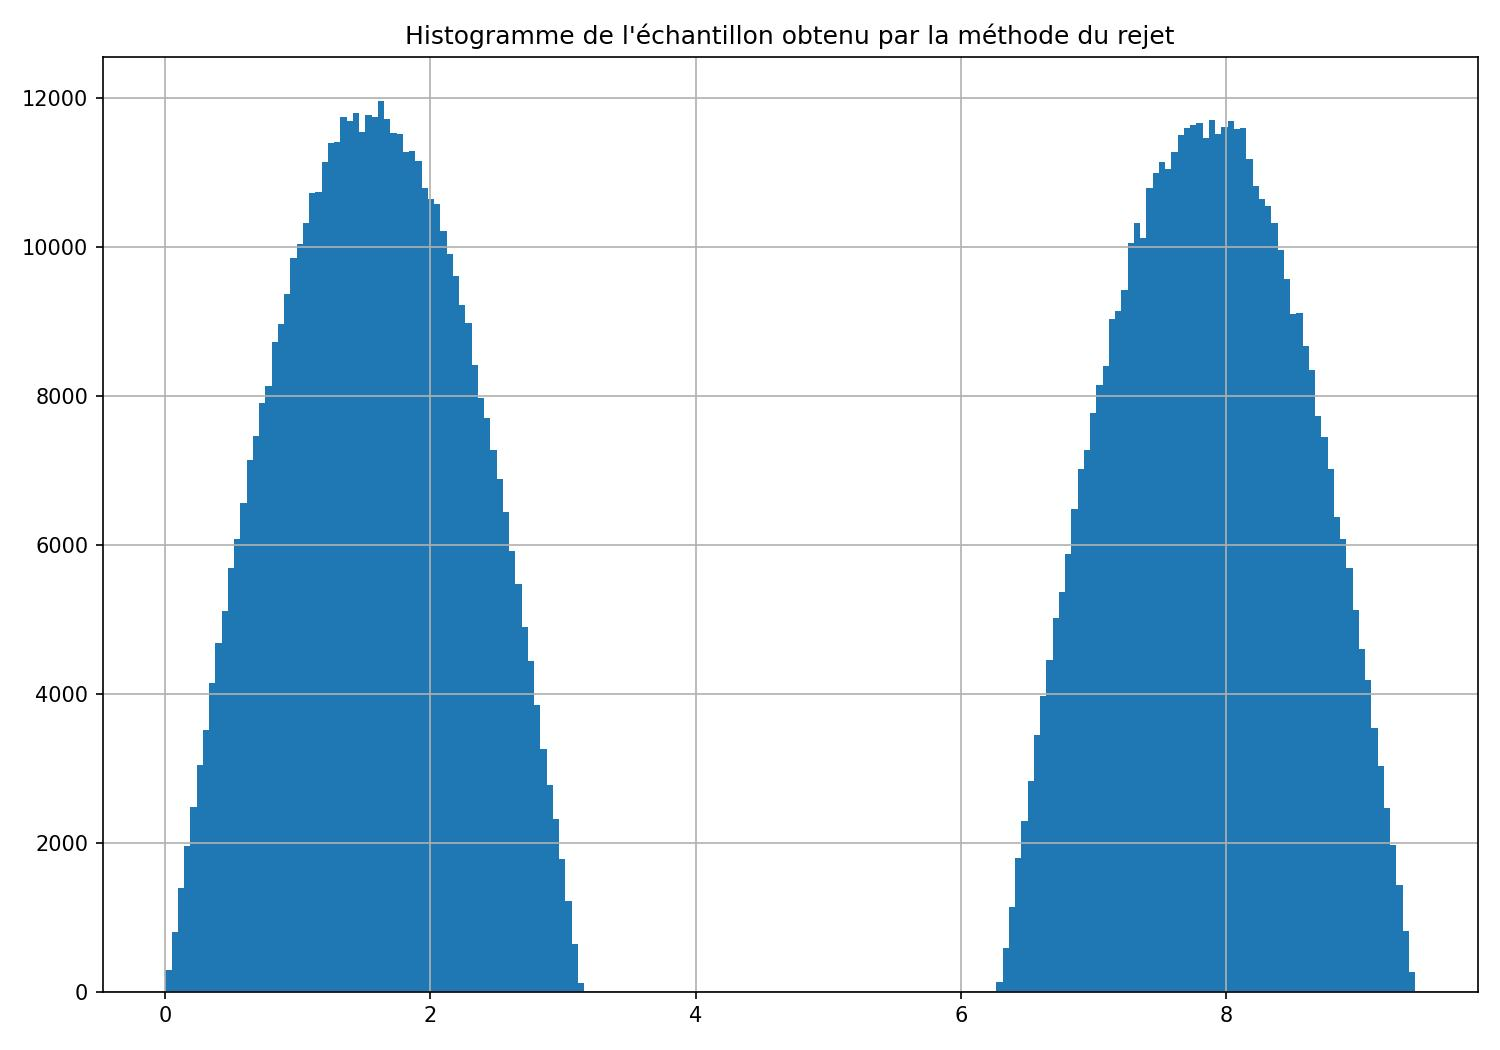
\includegraphics[width=0.7\textwidth]{images/exercice_rejet_2.jpg}
                    \caption{Histogramme de l'échantillon d'une distribution suivant la loi sinusoïdale demandée}
                    \label{fig:exercice_rejet_2}
                \end{figure}
    

    \section{Simulation Monte Carlo}
        \subsection{Exemple classique}
            \subsubsection{Estimation d'une intégrale définie}

        \subsection{Étude statistique d'un système dynamique stochastique}
    
    \section{Exercices}
\chapter{Simulations à évènements discrets}
    \section{Introduction}
        Les simulations Monte Carlo présentées dans le chapitre précédent sont largement utilisées dans la modélisation de systèmes dans lesquels les entités (par exemple des clients, des tâches, des véhicules…) attendent leur tour pour accéder à un service ou une ressource limitée. Ces systèmes sont modélisés par des files d'attentes. La file d'attente est caractérisée par plusieurs paramètres, comme le taux d'arrivée des entités, la capacité de la file, la discipline de service (par exemple, premier arrivé, premier servi), et le taux de service. Dans les simulations Monte Carlo, ces caractéristiques sont représentées de manière stochastique, avec des temps d'arrivée et de service qui suivent des distributions de probabilité prédéfinies. Chaque itération de la simulation implique alors la génération de ces temps aléatoires, permettant de simuler le comportement de la file d'attente sous différents scénarios d'incertitude. Cela permet d'estimer des métriques de performance comme le temps moyen d'attente, la longueur moyenne de la file, et le taux d'utilisation des serveurs, qui sont essentiels pour optimiser les systèmes en file d'attente dans des domaines comme les télécommunications, les transports, et la gestion de stocks.
    
        \codeword{SimPy} (\cite{Simpy2023}), une bibliothèque Python orientée vers la simulation de processus discrets, permet de modéliser des entités (comme des machines, des clients, des événements) dans un système avec des routines qui évoluent au fil du temps. Pour y intégrer une simulation Monte Carlo, on peut utiliser des tirages aléatoires pour simuler l'incertitude dans les paramètres du système, comme les temps de service ou d'arrivée, et observer des milliers de scénarios différents. L’objectif est d’analyser les sorties d’un système en fonction de distributions probabilistes sur ces paramètres incertains.

    \section{File d'attente}
        \begin{definition}{Notation de Kendall}
            La notation de Kendall $A/S/C/K/m$ définit une \textbf{file d'attente}, où chaque paramètre spécifie certaines caractéristiques de la file. Le paramètre $A$ indique la loi de probabilité des instants d'arrivées, $S$ indique la loi de probabilité de la durée du service, $C$ indique le nombre de serveurs, $K$ est la capacité totale du système et $m$ indique la population totale de clients.
        \end{definition}
        Ce modèle de file est utilisé pour analyser des systèmes dans lesquels les arrivées sont aléatoires et indépendantes, le service est fourni par un unique serveur, et il n'y a pas de restriction de place pour la file d'attente. Le comportement de la file d'attente peut être analysé à l'aide de diverses métriques, telles que la probabilité d'avoir $n$ clients dans le système, le temps moyen dans la file et le nombre moyen de clients.

        \subsection{Simulation de file d'attente en Python}
            Comme expliqué précédemment, \codeword{SimPy} est une bibliothèque Python conçue pour la simulation de processus à événements discrets. Elle permet, notamment, de simuler des processus dans des systèmes stochastiques où les événements se produisent de manière aléatoire, comme dans les files d'attente. La modélisation de files d'attente est un excellent exemple d'application des simulations Monte Carlo, car elle repose sur des événements déclenchés par des arrivées et des départs aléatoires de clients, et les simulations Monte Carlo permettent d'étudier cet aspect aléatoire.

        \subsection{File d'attente à client unique}
            Le cas le plus trivial correspond au cas où un client arrive après un temps aléatoire, attend quelques secondes (dans l'exemple suivant, $5$), et puis repart. On remarquera que cette file d'attente est peut-être un peu trop simplifiée par rapport à la réalité. L'action de rentrer, attendre, et sortir peut être modélisée par un \texttt{processus}. En \codeword{SimPy}, ceci peut être modélisé par le code suivant:
            \inputminted{python}{codes/client_unique.py}
            On y a défini un \codeword{Environment}, dans lequel différents \textit{processus} peuvent avoir lieu. On y a défini une classe \codeword{Client}, contenant une seule méthode, \codeword{enter}. Notez l'utilisation du mot-clé \codeword{yield}: celui-ci est à la base de la notion de générateur\footnote{Testez, pour mieux comprendre l'utilisation de ce mot clé, le code suivant:
            \inputminted[fontsize=\tiny]{python}{codes/yield.py}}. Ainsi, la méthode \codeword{enter} définit un générateur, qui déclenche un \codeword{Event} après un temps défini par \codeword{timeout}. Lorsque cet évènement est déclenché, le client rentre, et un message s'affiche. À la ligne suivante, on produit un déclencheur après un second \codeword{timeout}. Lorsque le temps est écoulé, le client sort.
            La méthode \codeword{enter} est ajoutée à l'environnement en tant que processus au moyen de la fonction \codeword{env.process(func)}, appelée dans la méthode \codeword{__init__()}. Finalement, la simulation est lancée grâce à la ligne \codeword{env.run(until=t)}, où \texttt{t} est le temps total de simulation.
            
        \subsection{File d'attente à serveur unique}
            En \codeword{SimPy}, la notion de serveur peut être modélisée par un objet de type \codeword{Resource}. Une ressource est définie par une certaine capacité $c$, qui dans le cas d'un serveur unique, vaut $1$. Pas plus d'un client ne peut accéder à la ressource à la fois: les clients excédants doivent attendre que la ressource se libère pour y accéder. Le code suivant montre comment utiliser la notion de ressource:
            \inputminted{python}{codes/serveur_unique.py}

        \subsection{File d'attente à serveur multiple}
            Si l'on adapte le code précédent pour accepter une capacité $c>1$, alors la ressource peut être utilisée par plusieurs clients en même temps:
            \inputminted{python}{codes/serveur_multiple.py}

        \subsection{Statistiques de simulation}
            Nous savons maintenant réaliser des simulations de files d'attentes. Il est intéressant de récupérer diverses statistiques qui résultent de l'exécution des simulations. Le code suivant montre comment on peut récupérer le temps de service pour chaque client. Dans ce code, le temps de service est une variable aléatoire qui suit une loi exponentielle négative, parfois appelée \textit{loi Markovienne}. Pour cette raison, dans la notation de Kendall, la file modélisée est notée $M/M/2/\infty/5$.
            \inputminted{python}{codes/statistiques_de_service.py}
            Seulement, cette simulation ne nous donne le temps d'attente que de $5$ clients. Si l'on répète la simulation un grand nombre de fois, on peut ajouter à la liste contenant les mesures tous les temps de service de chacune des simulations et donner un aperçu bien plus informatif. Ce processus se nomme \textbf{simulation Monte Carlo}.
            \begin{definition}{Simulation Monte Carlo}
                La simulation Monte Carlo est une méthode numérique permettant d'estimer des solutions pour des problèmes complexes en générant un grand nombre de scénarios aléatoires. En modélisant les variables du système selon leurs distributions de probabilité, elle permet de produire des estimations statistiques sur les résultats d'intérêt.
            \end{definition}
            Le code peut alors être adapté: 
            \inputminted{python}{codes/statistiques_de_service_2.py} et le résultat est donné en figure \ref{fig:statistiques_de_service}. On voit clairement que les mesures suivent une loi exponentielle négative.
            \begin{figure}
                \centering
                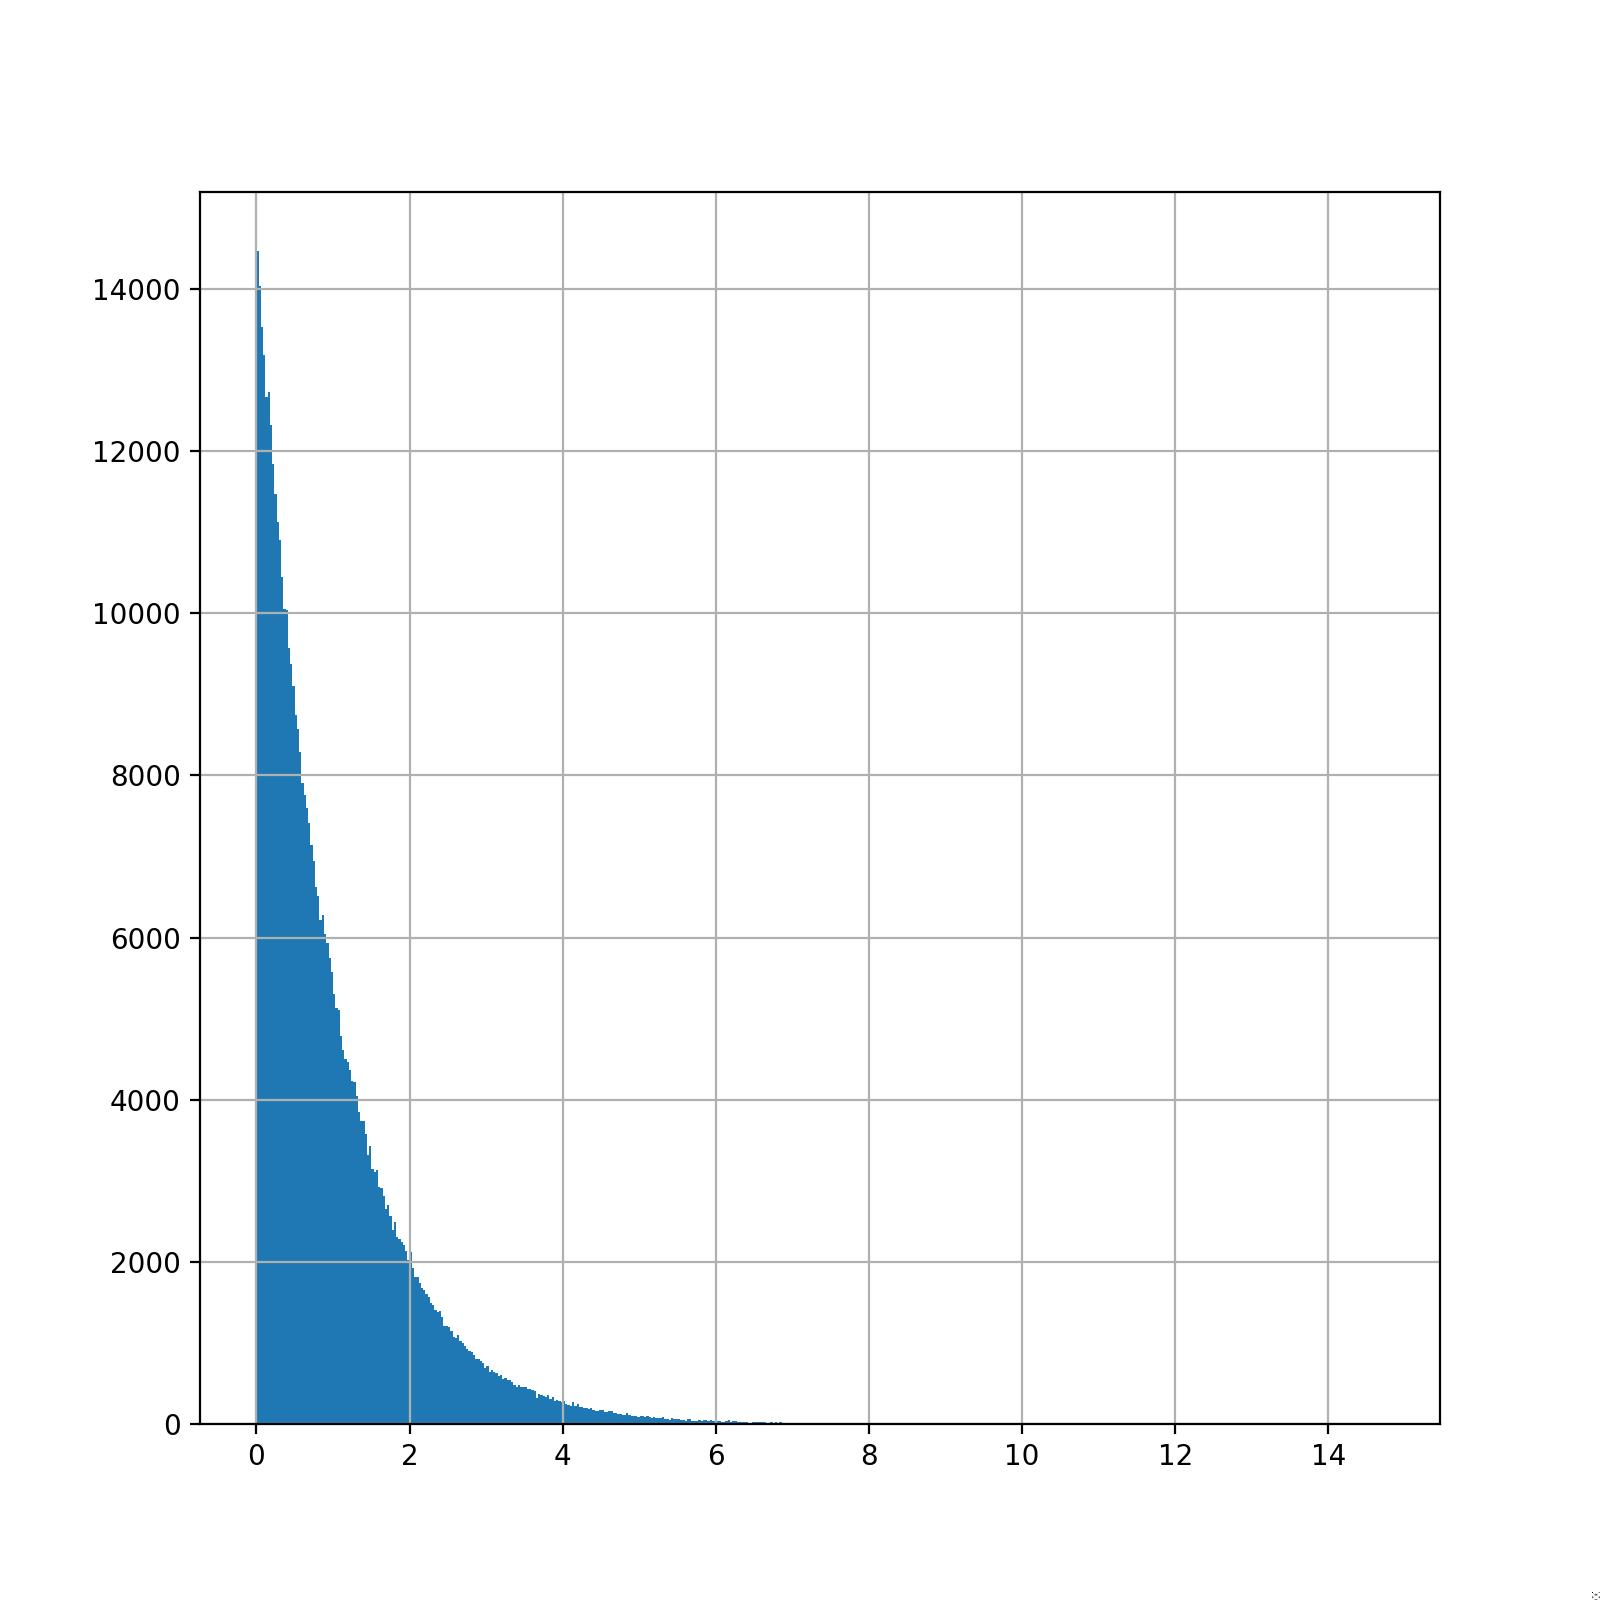
\includegraphics[width=\textwidth]{images/statistiques_de_service.jpg}
                \caption{Statistiques de service.}
                \label{fig:statistiques_de_service}
            \end{figure}
            
    \section{Exercice}
        On veut modéliser un service de charge de véhicules électriques. Le parc possède $4$ véhicules qui peuvent être loués de $8h$ à $22h$. Les véhicules ont une autonomie de $1h$ après lequel ils doivent être mis à charger jusqu'à charge complète. Le temps de charge $c$ suit une loi Markovienne de paramètre $\lambda = 1.5$. Les clients arrivent au magasin l'un après l'autre, avec un intervalle de temps les séparant qui suit une loi Markovienne de paramètre $\lambda = 0.2$. Ils louent un véhicule, si disponible, pour une durée qui suit une loi Markovienne de paramètre $\lambda=0.05$, et attendent sinon. 
        \begin{exercise}{Exercice 1}
            Formulez ce problème sous forme de file d'attente en suivant la notation de Kendall.
        \end{exercise}
        \begin{exercise}{Exercice 2}
            Modélisez la situation à l'aide de la librairie \codeword{SimPy}.
        \end{exercise}
        \begin{exercise}{Exercice 3}
            Déterminez, à l'aide d'une simulation Monte Carlo, la distribution et la moyenne du temps d'attente d'un client avant d'obtenir un véhicule.
        \end{exercise}
        \begin{exercise}{Exercice 4}
            Déterminez, à l'aide d'une simulation Monte Carlo, la distribution et la moyenne du nombre de recharges d'un véhicule.
        \end{exercise}

        Pour formuler le problème en utilisant la notation de Kendall, nous devons identifier les éléments suivants:
        \begin{itemize}
            \item type de la distribution d'arrivée des clients: les arrivées suivent une loi Markovienne marquée $M$~;
            \item type de la distribution du service (temps de location des véhicules) : le temps de location suit une loi Markovienne notée $M$~;
            \item nombre de serveurs (véhicules disponibles): $4$~;
            \item taille de la file d'attente: les clients attendent si aucun véhicule n'est disponible, donc la taille de la file d'attente est potentiellement infinie~;
            \item population : le nombre de clients potentiels est également supposé infini.
        \end{itemize}
        La notation de Kendall pour cette file d'attente est donc $M/M/4/\infty/\infty$.
        La solution aux exercices $2$, $3$ et $4$ est donnée dans le code
        \inputminted{python}{codes/charge.py}
\chapter{Conclusion}
    Ce syllabus a été conçu pour vous initier à l'art de la Modélisation et de la Simulation numérique des systèmes dynamiques. À travers les chapitres abordés, vous avez appris à résoudre différents types d'équations différentielles, à analyser des comportements de systèmes complexes, et à simuler numériquement des processus dynamiques en utilisant des outils informatiques.
    
    En modélisant divers phénomènes et en apprenant à interpréter les résultats des simulations, vous avez découvert comment les mathématiques et l'informatique peuvent nous permettre de représenter et de manipuler des systèmes complexes. Ces compétences vous placent maintenant en excellente position pour aborder des domaines encore plus avancés, où l'incertitude et les données jouent un rôle central.
    
    La suite naturelle de ce cours se trouve au sein du cours de \textit{Statistical Foundations of Machine Learning}. Dans ce cours, vous passerez de la simulation numérique et de la modélisation déterministe à l'inférence statistique et à la recherche de modèles prédictifs. Vous y apprendrez à modéliser des comportements non plus uniquement à partir de lois physiques, mais à partir de données, en employant des techniques statistiques pour estimer les paramètres et structures des modèles.
    
    Ce passage de la modélisation de systèmes déterministes à l'inférence statistique vous permettra de développer une compréhension encore plus fine des processus complexes, en apprenant à exploiter les données pour construire des modèles prédictifs et explicatifs. Ainsi, vous serez équipé pour répondre aux défis modernes posés par les grands ensembles de données et les systèmes incertains.
    
    Nous espérons que ce syllabus vous a non seulement transmis des connaissances pratiques et théoriques, mais aussi une intuition pour explorer plus avant le monde des systèmes dynamiques. Continuez à expérimenter, à questionner et à appliquer ces concepts, car la modélisation et la simulation numérique sont des outils fondamentaux pour une carrière en sciences informatiques. En vous souhaitant un apprentissage riche et stimulant dans la suite de vos études !

\chapter{Notation Sheet}
On note
\begin{itemize}
    \item Un nombre par une lettre minuscule ($x$, $a$, \ldots)
    \item Un vecteur par une lettre minuscule chapeautée d'une flèche ($\overrightarrow{v}$, $\overrightarrow{y}$, \ldots)
    \item Une matrice par une lettre majuscule ($A$, $X$, \ldots)
    \item Une fonction par une lettre minuscule suivie de parenthèses ($f(x)$, $g(\overrightarrow{a})$, \ldots)
    \item La dérivée d'une fonction, en forme longue, par l'opérateur $\dd $ ($\frac{f(x)}{\dd x}$, $\frac{g(a)}{\dd a}$, \ldots), 
    \item Ou, en forme courte, par l'opérateur $\dot{}$ ($\dot{f}(x)$, $\dot{g}(\overrightarrow{a})$, \ldots)
\end{itemize}
\newpage
\listoffigures
\newpage
\printbibliography

\end{document}
